\documentclass[runningheads]{llncs}

\usepackage[utf8]{inputenc}
\usepackage[T1]{fontenc}
\usepackage{alphabeta}
\usepackage{graphicx}
\usepackage{mathtools}
\usepackage{amssymb}
\usepackage{amsmath}
\usepackage{amsfonts}
\usepackage{hyperref}
\usepackage[conor,links]{agda}
\usepackage{bbm}
\usepackage{newunicodechar}
\usepackage{minted}
\usepackage{xcolor}
\usepackage{tikz}

\renewcommand{\fcolorbox}[4][]{#4}
\definecolor{mgreen}{HTML}{008000}
\newcommand{\inl}[1]{\mintinline[escapeinside=||]{haskell}{#1}}
\newcommand{\mono}[1]{\footnotesize{\ttfamily{#1}}}
\newcommand{\Fo}[0]{F$_\text{O}$} 
\newcommand{\Inst}[0]{\textcolor{mgreen}{inst}}
\newcommand{\Decl}[0]{\textcolor{mgreen}{decl}}
\newcommand{\Blk}[1]{\textcolor{black}{#1}}
\makeatletter
\newcommand{\lambdabar}{\ensuremath{\mathchoice
  {\smash@bar\textfont\displaystyle{0.25}{1.2}\lambda}
  {\smash@bar\textfont\textstyle{0.25}{1.2}\lambda}
  {\smash@bar\scriptfont\scriptstyle{0.25}{1.2}\lambda}
  {\smash@bar\scriptscriptfont\scriptscriptstyle{0.25}{1.2}\lambda}
}}
\newcommand{\smash@bar}[4]{%
  \smash{\rlap{\raisebox{-#3\fontdimen5#10}{$\m@th#2\mkern#4mu\mathchar'26$}}}%
}
\newcommand{\Sym}[1]{\AgdaGeneralizable{#1}}
\newcommand{\Data}[1]{\AgdaDatatype{#1}}
\newcommand{\Constr}[1]{\AgdaInductiveConstructor{#1}}
\newcommand{\Prim}[1]{\AgdaPrimitive{#1}}
\makeatletter
\newcommand{\Scalecenter}[2][1]{\mathpalette\Scalecenter@{{#1}{#2}}}
\newcommand{\Scalecenter@}[2]{\Scalecenter@@#1#2}
\newcommand{\Scalecenter@@}[3]{%
  \vcenter{\hbox{\scalebox{#2}{$\m@th#1#3$}}}%
}
\makeatother

\newcommand{\smallblacktriangleright}{%
  \Scalecenter[0.75]{\blacktriangleright}%
}



\makeatother

\newunicodechar{λ}{\ensuremath{\mathnormal\lambda}}
\newunicodechar{Λ}{\ensuremath{\mathnormal\Lambda}}
\newunicodechar{ƛ}{\ensuremath{\lbar}}
\newunicodechar{τ}{\ensuremath{\mathnormal\tau}}
\newunicodechar{ℕ}{\ensuremath{\mathbb{N}}}
\newunicodechar{∶}{\ensuremath{:}}
\newunicodechar{≡}{\ensuremath{\equiv}}
\newunicodechar{∀}{\ensuremath{\forall}}
\newunicodechar{⊤}{\ensuremath{\top}}
\newunicodechar{⊥}{\ensuremath{\bot}}
\newunicodechar{₁}{\ensuremath{_1}}
\newunicodechar{₂}{\ensuremath{_2}}
\newunicodechar{∈}{\ensuremath{\in}}
\newunicodechar{′}{\ensuremath{'}}
\newunicodechar{·}{\ensuremath{\cdot}}
\newunicodechar{⊎}{\ensuremath{\uplus}}
\newunicodechar{∷}{\ensuremath{::}}
\newunicodechar{▷}{\ensuremath{\triangleright}}
\newunicodechar{ᶜ}{\ensuremath{^c}}
\newunicodechar{⊎}{\ensuremath{\uplus}}
\newunicodechar{×}{\ensuremath{\times}}
\newunicodechar{Σ}{\ensuremath{\Sigma}}
\newunicodechar{∃}{\ensuremath{\exists}}
\newunicodechar{≢}{\ensuremath{\not\equiv}}
\newunicodechar{∘}{\ensuremath{\circ}}
\newunicodechar{α}{\ensuremath{\mathnormal\alpha}}
\newunicodechar{⇒}{\ensuremath{\Rightarrow}}
\newunicodechar{→}{\ensuremath{\rightarrow}}
\newunicodechar{·}{\ensuremath{\cdot}}
\newunicodechar{•}{\ensuremath{\bullet}}
\newunicodechar{∶}{\ensuremath{:}}
\newunicodechar{∀}{\ensuremath{\forall}}
\newunicodechar{ρ}{\ensuremath{\mathnormal\rho}}
\newunicodechar{σ}{\ensuremath{\mathnormal\sigma}}
\newunicodechar{∅}{\ensuremath{\emptyset}}
\newunicodechar{▶}{\ensuremath{\blacktriangleright}}
\newunicodechar{▸}{\ensuremath{\smallblacktriangleright}}
\newunicodechar{⊘}{\ensuremath{\oslash}}
\newunicodechar{Γ}{\ensuremath{\mathnormal\Gamma}}
\newunicodechar{⊢}{\ensuremath{\vdash}}
\newunicodechar{ᵣ}{\ensuremath{_r}}
\newunicodechar{ₛ}{\ensuremath{_s}}
\newunicodechar{ᴼ}{\ensuremath{^\text{O}}}
\newunicodechar{⇝}{\ensuremath{\rightsquigarrow}}
\newunicodechar{≐}{\ensuremath{\doteq}}


\title{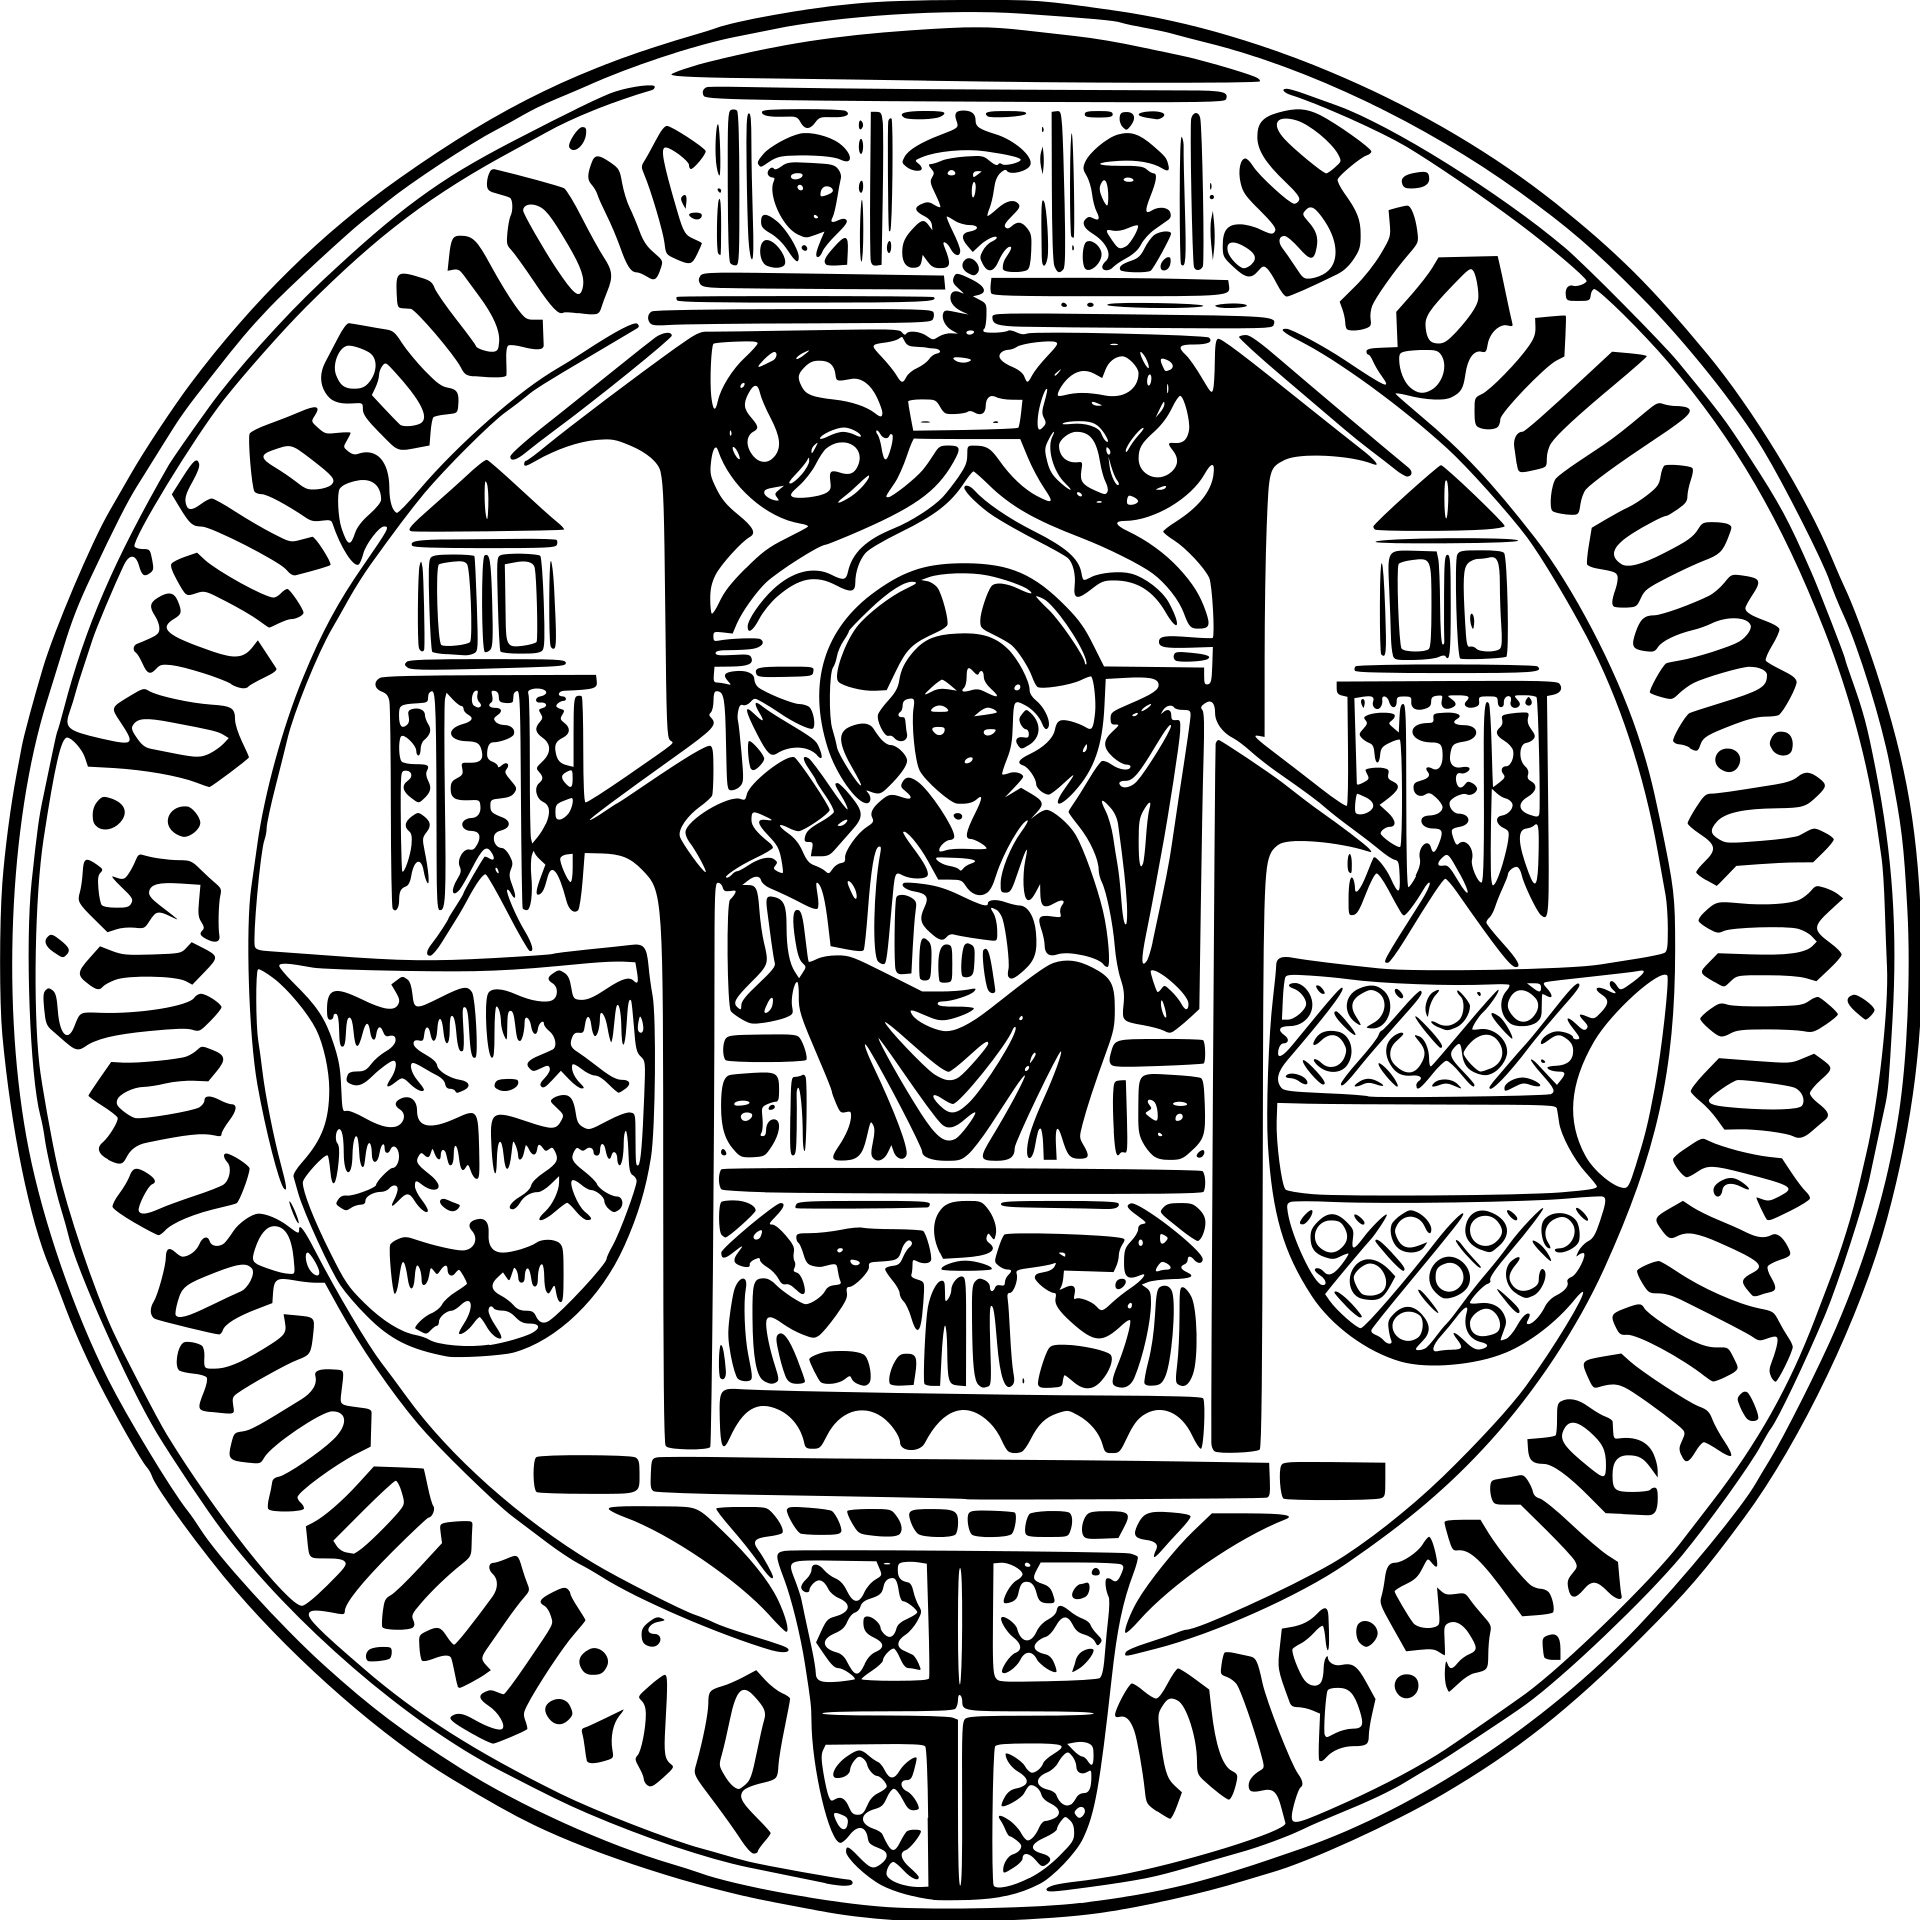
\includegraphics[width=0.75\textwidth]{logo.png}~ 
\\[1cm]
Formal Proof of Type Preservation of the Dictionary Passing Transform for System F}
\titlerunning{Type Preservation Proof of the Dictionary Passing Transform for System F}
\institute{Chair of Programming Languages, University of Freiburg \\ \email{weidner@cs.uni-freiburg.de}}
\author{Marius Weidner}


\begin{document}

\let\oldaddcontentsline\addcontentsline
\def\addcontentsline#1#2#3{}
\maketitle
\def\addcontentsline#1#2#3{\oldaddcontentsline{#1}{#2}{#3}}


\noindent\makebox[\linewidth]{\bf{Bachelor Thesis}}
\\

\noindent\makebox[\linewidth]{Examiner: Prof. Dr. Peter Thiemann}
\noindent\makebox[\linewidth]{Advisor: Hannes Saffrich}

\begin{code}[hide]%
\>[0]\AgdaSymbol{\{-\#}\AgdaSpace{}%
\AgdaKeyword{OPTIONS}\AgdaSpace{}%
\AgdaPragma{--allow-unsolved-metas}\AgdaSpace{}%
\AgdaSymbol{\#-\}}\<%
\\
\>[0]\AgdaKeyword{open}\AgdaSpace{}%
\AgdaKeyword{import}\AgdaSpace{}%
\AgdaModule{Data.Unit}\AgdaSpace{}%
\AgdaKeyword{using}\AgdaSpace{}%
\AgdaSymbol{(}\AgdaRecord{⊤}\AgdaSymbol{;}\AgdaSpace{}%
\AgdaInductiveConstructor{tt}\AgdaSymbol{)}\<%
\\
\>[0]\AgdaKeyword{open}\AgdaSpace{}%
\AgdaKeyword{import}\AgdaSpace{}%
\AgdaModule{Data.Nat}\AgdaSpace{}%
\AgdaKeyword{using}\AgdaSpace{}%
\AgdaSymbol{(}\AgdaDatatype{ℕ}\AgdaSymbol{;}\AgdaSpace{}%
\AgdaInductiveConstructor{zero}\AgdaSymbol{;}\AgdaSpace{}%
\AgdaInductiveConstructor{suc}\AgdaSymbol{)}\<%
\\
\>[0]\AgdaKeyword{open}\AgdaSpace{}%
\AgdaKeyword{import}\AgdaSpace{}%
\AgdaModule{Data.List}\AgdaSpace{}%
\AgdaKeyword{using}\AgdaSpace{}%
\AgdaSymbol{(}\AgdaDatatype{List}\AgdaSymbol{;}\AgdaSpace{}%
\AgdaInductiveConstructor{[]}\AgdaSymbol{;}\AgdaSpace{}%
\AgdaOperator{\AgdaInductiveConstructor{\AgdaUnderscore{}∷\AgdaUnderscore{}}}\AgdaSymbol{;}\AgdaSpace{}%
\AgdaOperator{\AgdaFunction{\AgdaUnderscore{}++\AgdaUnderscore{}}}\AgdaSymbol{;}\AgdaSpace{}%
\AgdaFunction{drop}\AgdaSymbol{)}\<%
\\
\>[0]\AgdaKeyword{open}\AgdaSpace{}%
\AgdaKeyword{import}\AgdaSpace{}%
\AgdaModule{Data.List.Relation.Unary.Any}\AgdaSpace{}%
\AgdaKeyword{using}\AgdaSpace{}%
\AgdaSymbol{(}\AgdaInductiveConstructor{here}\AgdaSymbol{;}\AgdaSpace{}%
\AgdaInductiveConstructor{there}\AgdaSymbol{)}\<%
\\
\>[0]\AgdaKeyword{open}\AgdaSpace{}%
\AgdaKeyword{import}\AgdaSpace{}%
\AgdaModule{Data.List.Membership.Propositional}\AgdaSpace{}%
\AgdaKeyword{using}\AgdaSpace{}%
\AgdaSymbol{(}\AgdaOperator{\AgdaFunction{\AgdaUnderscore{}∈\AgdaUnderscore{}}}\AgdaSymbol{)}\<%
\\
\>[0]\AgdaKeyword{open}\AgdaSpace{}%
\AgdaKeyword{import}\AgdaSpace{}%
\AgdaModule{Data.Sum.Base}\AgdaSpace{}%
\AgdaKeyword{using}\AgdaSpace{}%
\AgdaSymbol{(}\AgdaOperator{\AgdaDatatype{\AgdaUnderscore{}⊎\AgdaUnderscore{}}}\AgdaSymbol{;}\AgdaSpace{}%
\AgdaInductiveConstructor{inj₁}\AgdaSymbol{;}\AgdaSpace{}%
\AgdaInductiveConstructor{inj₂}\AgdaSymbol{)}\<%
\\
\>[0]\AgdaKeyword{open}\AgdaSpace{}%
\AgdaKeyword{import}\AgdaSpace{}%
\AgdaModule{Data.Product}\AgdaSpace{}%
\AgdaKeyword{using}\AgdaSpace{}%
\AgdaSymbol{(}\AgdaOperator{\AgdaFunction{\AgdaUnderscore{}×\AgdaUnderscore{}}}\AgdaSymbol{;}\AgdaSpace{}%
\AgdaOperator{\AgdaInductiveConstructor{\AgdaUnderscore{},\AgdaUnderscore{}}}\AgdaSymbol{;}\AgdaSpace{}%
\AgdaFunction{Σ-syntax}\AgdaSymbol{;}\AgdaSpace{}%
\AgdaFunction{∃-syntax}\AgdaSymbol{)}\<%
\\
\>[0]\AgdaKeyword{open}\AgdaSpace{}%
\AgdaKeyword{import}\AgdaSpace{}%
\AgdaModule{Relation.Binary.PropositionalEquality}\AgdaSpace{}%
\AgdaKeyword{using}\AgdaSpace{}%
\AgdaSymbol{(}\AgdaOperator{\AgdaDatatype{\AgdaUnderscore{}≡\AgdaUnderscore{}}}\AgdaSymbol{;}\AgdaSpace{}%
\AgdaInductiveConstructor{refl}\AgdaSymbol{;}\AgdaSpace{}%
\AgdaFunction{subst}\AgdaSymbol{;}\AgdaSpace{}%
\AgdaFunction{sym}\AgdaSymbol{;}\AgdaSpace{}%
\AgdaFunction{cong}\AgdaSymbol{;}\AgdaSpace{}%
\AgdaFunction{cong₂}\AgdaSymbol{;}\AgdaSpace{}%
\AgdaFunction{trans}\AgdaSymbol{;}\AgdaSpace{}%
\AgdaKeyword{module}\AgdaSpace{}%
\AgdaModule{≡-Reasoning}\AgdaSymbol{)}\<%
\\
\>[0]\AgdaKeyword{open}\AgdaSpace{}%
\AgdaKeyword{import}\AgdaSpace{}%
\AgdaModule{Function}\AgdaSpace{}%
\AgdaKeyword{using}\AgdaSpace{}%
\AgdaSymbol{(}\AgdaFunction{id}\AgdaSymbol{;}\AgdaSpace{}%
\AgdaOperator{\AgdaFunction{\AgdaUnderscore{}∘\AgdaUnderscore{}}}\AgdaSymbol{)}\<%
\\
\>[0]\AgdaKeyword{open}\AgdaSpace{}%
\AgdaModule{≡-Reasoning}\<%
\\
%
\\[\AgdaEmptyExtraSkip]%
\>[0]\AgdaKeyword{module}\AgdaSpace{}%
\AgdaModule{SystemF}\AgdaSpace{}%
\AgdaKeyword{where}\<%
\\
%
\\[\AgdaEmptyExtraSkip]%
\>[0]\AgdaComment{--\ Sorts\ --------------------------------------------------------------------------------}\<%
\\
%
\\[\AgdaEmptyExtraSkip]%
\>[0]\AgdaKeyword{data}\AgdaSpace{}%
\AgdaDatatype{Bindable}\AgdaSpace{}%
\AgdaSymbol{:}\AgdaSpace{}%
\AgdaPrimitive{Set}\AgdaSpace{}%
\AgdaKeyword{where}\<%
\\
\>[0][@{}l@{\AgdaIndent{0}}]%
\>[2]\AgdaInductiveConstructor{B}\AgdaSpace{}%
\AgdaSymbol{:}\AgdaSpace{}%
\AgdaDatatype{Bindable}\<%
\\
%
\>[2]\AgdaInductiveConstructor{¬B}\AgdaSpace{}%
\AgdaSymbol{:}\AgdaSpace{}%
\AgdaDatatype{Bindable}\<%
\end{code}
\newcommand{\FSort}[0]{\begin{code}%
\>[0]\AgdaKeyword{data}\AgdaSpace{}%
\AgdaDatatype{Sort}\AgdaSpace{}%
\AgdaSymbol{:}\AgdaSpace{}%
\AgdaDatatype{Bindable}\AgdaSpace{}%
\AgdaSymbol{→}\AgdaSpace{}%
\AgdaPrimitive{Set}\AgdaSpace{}%
\AgdaKeyword{where}\<%
\\
\>[0][@{}l@{\AgdaIndent{0}}]%
\>[2]\AgdaInductiveConstructor{eₛ}%
\>[6]\AgdaSymbol{:}\AgdaSpace{}%
\AgdaDatatype{Sort}\AgdaSpace{}%
\AgdaInductiveConstructor{B}\<%
\\
%
\>[2]\AgdaInductiveConstructor{τₛ}%
\>[6]\AgdaSymbol{:}\AgdaSpace{}%
\AgdaDatatype{Sort}\AgdaSpace{}%
\AgdaInductiveConstructor{B}\<%
\\
%
\>[2]\AgdaInductiveConstructor{κₛ}%
\>[6]\AgdaSymbol{:}\AgdaSpace{}%
\AgdaDatatype{Sort}\AgdaSpace{}%
\AgdaInductiveConstructor{¬B}\<%
\\
%
\\[\AgdaEmptyExtraSkip]%
\>[0]\AgdaFunction{Sorts}\AgdaSpace{}%
\AgdaSymbol{:}\AgdaSpace{}%
\AgdaPrimitive{Set}\<%
\\
\>[0]\AgdaFunction{Sorts}\AgdaSpace{}%
\AgdaSymbol{=}\AgdaSpace{}%
\AgdaDatatype{List}\AgdaSpace{}%
\AgdaSymbol{(}\AgdaDatatype{Sort}\AgdaSpace{}%
\AgdaInductiveConstructor{B}\AgdaSymbol{)}\<%
\end{code}}
\begin{code}[hide]%
\>[0]\AgdaKeyword{infix}\AgdaSpace{}%
\AgdaNumber{25}\AgdaSpace{}%
\AgdaOperator{\AgdaInductiveConstructor{\AgdaUnderscore{}▷\AgdaUnderscore{}}}\AgdaSpace{}%
\AgdaOperator{\AgdaFunction{\AgdaUnderscore{}▷▷\AgdaUnderscore{}}}\<%
\\
\>[0]\AgdaKeyword{pattern}\AgdaSpace{}%
\AgdaOperator{\AgdaInductiveConstructor{\AgdaUnderscore{}▷\AgdaUnderscore{}}}\AgdaSpace{}%
\AgdaBound{xs}\AgdaSpace{}%
\AgdaBound{x}\AgdaSpace{}%
\AgdaSymbol{=}\AgdaSpace{}%
\AgdaBound{x}\AgdaSpace{}%
\AgdaOperator{\AgdaInductiveConstructor{∷}}\AgdaSpace{}%
\AgdaBound{xs}\<%
\\
\>[0]\AgdaOperator{\AgdaFunction{\AgdaUnderscore{}▷▷\AgdaUnderscore{}}}\AgdaSpace{}%
\AgdaSymbol{:}\AgdaSpace{}%
\AgdaSymbol{\{}\AgdaBound{A}\AgdaSpace{}%
\AgdaSymbol{:}\AgdaSpace{}%
\AgdaPrimitive{Set}\AgdaSymbol{\}}\AgdaSpace{}%
\AgdaSymbol{→}\AgdaSpace{}%
\AgdaDatatype{List}\AgdaSpace{}%
\AgdaBound{A}\AgdaSpace{}%
\AgdaSymbol{→}\AgdaSpace{}%
\AgdaDatatype{List}\AgdaSpace{}%
\AgdaBound{A}\AgdaSpace{}%
\AgdaSymbol{→}\AgdaSpace{}%
\AgdaDatatype{List}\AgdaSpace{}%
\AgdaBound{A}\<%
\\
\>[0]\AgdaBound{xs}\AgdaSpace{}%
\AgdaOperator{\AgdaFunction{▷▷}}\AgdaSpace{}%
\AgdaBound{ys}\AgdaSpace{}%
\AgdaSymbol{=}\AgdaSpace{}%
\AgdaBound{ys}\AgdaSpace{}%
\AgdaOperator{\AgdaFunction{++}}\AgdaSpace{}%
\AgdaBound{xs}\<%
\\
%
\\[\AgdaEmptyExtraSkip]%
\>[0]\AgdaKeyword{variable}\<%
\\
\>[0][@{}l@{\AgdaIndent{0}}]%
\>[2]\AgdaGeneralizable{r}\AgdaSpace{}%
\AgdaGeneralizable{r'}\AgdaSpace{}%
\AgdaGeneralizable{r''}\AgdaSpace{}%
\AgdaGeneralizable{r₁}\AgdaSpace{}%
\AgdaGeneralizable{r₂}\AgdaSpace{}%
\AgdaSymbol{:}\AgdaSpace{}%
\AgdaDatatype{Bindable}\<%
\\
%
\>[2]\AgdaGeneralizable{s}\AgdaSpace{}%
\AgdaGeneralizable{s'}\AgdaSpace{}%
\AgdaGeneralizable{s''}\AgdaSpace{}%
\AgdaGeneralizable{s₁}\AgdaSpace{}%
\AgdaGeneralizable{s₂}\AgdaSpace{}%
\AgdaSymbol{:}\AgdaSpace{}%
\AgdaDatatype{Sort}\AgdaSpace{}%
\AgdaGeneralizable{r}\<%
\\
%
\>[2]\AgdaGeneralizable{S}\AgdaSpace{}%
\AgdaGeneralizable{S'}\AgdaSpace{}%
\AgdaGeneralizable{S''}\AgdaSpace{}%
\AgdaGeneralizable{S₁}\AgdaSpace{}%
\AgdaGeneralizable{S₂}\AgdaSpace{}%
\AgdaSymbol{:}\AgdaSpace{}%
\AgdaFunction{Sorts}\<%
\\
%
\>[2]\AgdaGeneralizable{x}\AgdaSpace{}%
\AgdaGeneralizable{x'}\AgdaSpace{}%
\AgdaGeneralizable{x''}\AgdaSpace{}%
\AgdaGeneralizable{x₁}\AgdaSpace{}%
\AgdaGeneralizable{x₂}\AgdaSpace{}%
\AgdaSymbol{:}\AgdaSpace{}%
\AgdaInductiveConstructor{eₛ}\AgdaSpace{}%
\AgdaOperator{\AgdaFunction{∈}}\AgdaSpace{}%
\AgdaGeneralizable{S}\<%
\\
%
\>[2]\AgdaGeneralizable{α}\AgdaSpace{}%
\AgdaGeneralizable{α'}\AgdaSpace{}%
\AgdaGeneralizable{α''}\AgdaSpace{}%
\AgdaGeneralizable{α₁}\AgdaSpace{}%
\AgdaGeneralizable{α₂}\AgdaSpace{}%
\AgdaSymbol{:}\AgdaSpace{}%
\AgdaInductiveConstructor{τₛ}\AgdaSpace{}%
\AgdaOperator{\AgdaFunction{∈}}\AgdaSpace{}%
\AgdaGeneralizable{S}\<%
\\
%
\\[\AgdaEmptyExtraSkip]%
\>[0]\AgdaComment{--\ Syntax\ -------------------------------------------------------------------------------}\<%
\\
%
\\[\AgdaEmptyExtraSkip]%
\>[0]\AgdaKeyword{infixr}\AgdaSpace{}%
\AgdaNumber{4}\AgdaSpace{}%
\AgdaOperator{\AgdaInductiveConstructor{λ`x→\AgdaUnderscore{}}}\AgdaSpace{}%
\AgdaOperator{\AgdaInductiveConstructor{Λ`α→\AgdaUnderscore{}}}\AgdaSpace{}%
\AgdaOperator{\AgdaInductiveConstructor{let`x=\AgdaUnderscore{}`in\AgdaUnderscore{}}}\AgdaSpace{}%
\AgdaOperator{\AgdaInductiveConstructor{∀`α\AgdaUnderscore{}}}\<%
\\
\>[0]\AgdaKeyword{infixr}\AgdaSpace{}%
\AgdaNumber{5}\AgdaSpace{}%
\AgdaOperator{\AgdaInductiveConstructor{\AgdaUnderscore{}⇒\AgdaUnderscore{}}}\AgdaSpace{}%
\AgdaOperator{\AgdaInductiveConstructor{\AgdaUnderscore{}·\AgdaUnderscore{}}}\AgdaSpace{}%
\AgdaOperator{\AgdaInductiveConstructor{\AgdaUnderscore{}•\AgdaUnderscore{}}}\<%
\\
\>[0]\AgdaKeyword{infix}%
\>[7]\AgdaNumber{6}\AgdaSpace{}%
\AgdaOperator{\AgdaInductiveConstructor{`\AgdaUnderscore{}}}\<%
\end{code}
\newcommand{\FTerm}[0]{\begin{code}%
\>[0]\AgdaKeyword{data}\AgdaSpace{}%
\AgdaDatatype{Term}\AgdaSpace{}%
\AgdaSymbol{:}\AgdaSpace{}%
\AgdaFunction{Sorts}\AgdaSpace{}%
\AgdaSymbol{→}\AgdaSpace{}%
\AgdaDatatype{Sort}\AgdaSpace{}%
\AgdaGeneralizable{r}\AgdaSpace{}%
\AgdaSymbol{→}\AgdaSpace{}%
\AgdaPrimitive{Set}\AgdaSpace{}%
\AgdaKeyword{where}\<%
\\
\>[0][@{}l@{\AgdaIndent{0}}]%
\>[2]\AgdaOperator{\AgdaInductiveConstructor{`\AgdaUnderscore{}}}%
\>[15]\AgdaSymbol{:}\AgdaSpace{}%
\AgdaGeneralizable{s}\AgdaSpace{}%
\AgdaOperator{\AgdaFunction{∈}}\AgdaSpace{}%
\AgdaGeneralizable{S}\AgdaSpace{}%
\AgdaSymbol{→}\AgdaSpace{}%
\AgdaDatatype{Term}\AgdaSpace{}%
\AgdaGeneralizable{S}\AgdaSpace{}%
\AgdaGeneralizable{s}\<%
\\
%
\>[2]\AgdaInductiveConstructor{tt}%
\>[15]\AgdaSymbol{:}\AgdaSpace{}%
\AgdaDatatype{Term}\AgdaSpace{}%
\AgdaGeneralizable{S}\AgdaSpace{}%
\AgdaInductiveConstructor{eₛ}\<%
\\
%
\>[2]\AgdaOperator{\AgdaInductiveConstructor{λ`x→\AgdaUnderscore{}}}%
\>[15]\AgdaSymbol{:}\AgdaSpace{}%
\AgdaDatatype{Term}\AgdaSpace{}%
\AgdaSymbol{(}\AgdaGeneralizable{S}\AgdaSpace{}%
\AgdaOperator{\AgdaInductiveConstructor{▷}}\AgdaSpace{}%
\AgdaInductiveConstructor{eₛ}\AgdaSymbol{)}\AgdaSpace{}%
\AgdaInductiveConstructor{eₛ}\AgdaSpace{}%
\AgdaSymbol{→}\AgdaSpace{}%
\AgdaDatatype{Term}\AgdaSpace{}%
\AgdaGeneralizable{S}\AgdaSpace{}%
\AgdaInductiveConstructor{eₛ}\<%
\\
%
\>[2]\AgdaOperator{\AgdaInductiveConstructor{Λ`α→\AgdaUnderscore{}}}%
\>[15]\AgdaSymbol{:}\AgdaSpace{}%
\AgdaDatatype{Term}\AgdaSpace{}%
\AgdaSymbol{(}\AgdaGeneralizable{S}\AgdaSpace{}%
\AgdaOperator{\AgdaInductiveConstructor{▷}}\AgdaSpace{}%
\AgdaInductiveConstructor{τₛ}\AgdaSymbol{)}\AgdaSpace{}%
\AgdaInductiveConstructor{eₛ}\AgdaSpace{}%
\AgdaSymbol{→}\AgdaSpace{}%
\AgdaDatatype{Term}\AgdaSpace{}%
\AgdaGeneralizable{S}\AgdaSpace{}%
\AgdaInductiveConstructor{eₛ}\<%
\\
%
\>[2]\AgdaOperator{\AgdaInductiveConstructor{\AgdaUnderscore{}·\AgdaUnderscore{}}}%
\>[15]\AgdaSymbol{:}\AgdaSpace{}%
\AgdaDatatype{Term}\AgdaSpace{}%
\AgdaGeneralizable{S}\AgdaSpace{}%
\AgdaInductiveConstructor{eₛ}\AgdaSpace{}%
\AgdaSymbol{→}\AgdaSpace{}%
\AgdaDatatype{Term}\AgdaSpace{}%
\AgdaGeneralizable{S}\AgdaSpace{}%
\AgdaInductiveConstructor{eₛ}\AgdaSpace{}%
\AgdaSymbol{→}\AgdaSpace{}%
\AgdaDatatype{Term}\AgdaSpace{}%
\AgdaGeneralizable{S}\AgdaSpace{}%
\AgdaInductiveConstructor{eₛ}\<%
\\
%
\>[2]\AgdaOperator{\AgdaInductiveConstructor{\AgdaUnderscore{}•\AgdaUnderscore{}}}%
\>[15]\AgdaSymbol{:}\AgdaSpace{}%
\AgdaDatatype{Term}\AgdaSpace{}%
\AgdaGeneralizable{S}\AgdaSpace{}%
\AgdaInductiveConstructor{eₛ}\AgdaSpace{}%
\AgdaSymbol{→}\AgdaSpace{}%
\AgdaDatatype{Term}\AgdaSpace{}%
\AgdaGeneralizable{S}\AgdaSpace{}%
\AgdaInductiveConstructor{τₛ}\AgdaSpace{}%
\AgdaSymbol{→}\AgdaSpace{}%
\AgdaDatatype{Term}\AgdaSpace{}%
\AgdaGeneralizable{S}\AgdaSpace{}%
\AgdaInductiveConstructor{eₛ}\<%
\\
%
\>[2]\AgdaOperator{\AgdaInductiveConstructor{let`x=\AgdaUnderscore{}`in\AgdaUnderscore{}}}%
\>[15]\AgdaSymbol{:}\AgdaSpace{}%
\AgdaDatatype{Term}\AgdaSpace{}%
\AgdaGeneralizable{S}\AgdaSpace{}%
\AgdaInductiveConstructor{eₛ}\AgdaSpace{}%
\AgdaSymbol{→}\AgdaSpace{}%
\AgdaDatatype{Term}\AgdaSpace{}%
\AgdaSymbol{(}\AgdaGeneralizable{S}\AgdaSpace{}%
\AgdaOperator{\AgdaInductiveConstructor{▷}}\AgdaSpace{}%
\AgdaInductiveConstructor{eₛ}\AgdaSymbol{)}\AgdaSpace{}%
\AgdaInductiveConstructor{eₛ}\AgdaSpace{}%
\AgdaSymbol{→}\AgdaSpace{}%
\AgdaDatatype{Term}\AgdaSpace{}%
\AgdaGeneralizable{S}\AgdaSpace{}%
\AgdaInductiveConstructor{eₛ}\<%
\\
%
\>[2]\AgdaInductiveConstructor{`⊤}%
\>[15]\AgdaSymbol{:}\AgdaSpace{}%
\AgdaDatatype{Term}\AgdaSpace{}%
\AgdaGeneralizable{S}\AgdaSpace{}%
\AgdaInductiveConstructor{τₛ}\<%
\\
%
\>[2]\AgdaOperator{\AgdaInductiveConstructor{\AgdaUnderscore{}⇒\AgdaUnderscore{}}}%
\>[15]\AgdaSymbol{:}\AgdaSpace{}%
\AgdaDatatype{Term}\AgdaSpace{}%
\AgdaGeneralizable{S}\AgdaSpace{}%
\AgdaInductiveConstructor{τₛ}\AgdaSpace{}%
\AgdaSymbol{→}\AgdaSpace{}%
\AgdaDatatype{Term}\AgdaSpace{}%
\AgdaGeneralizable{S}\AgdaSpace{}%
\AgdaInductiveConstructor{τₛ}\AgdaSpace{}%
\AgdaSymbol{→}\AgdaSpace{}%
\AgdaDatatype{Term}\AgdaSpace{}%
\AgdaGeneralizable{S}\AgdaSpace{}%
\AgdaInductiveConstructor{τₛ}\<%
\\
%
\>[2]\AgdaOperator{\AgdaInductiveConstructor{∀`α\AgdaUnderscore{}}}%
\>[15]\AgdaSymbol{:}\AgdaSpace{}%
\AgdaDatatype{Term}\AgdaSpace{}%
\AgdaSymbol{(}\AgdaGeneralizable{S}\AgdaSpace{}%
\AgdaOperator{\AgdaInductiveConstructor{▷}}\AgdaSpace{}%
\AgdaInductiveConstructor{τₛ}\AgdaSymbol{)}\AgdaSpace{}%
\AgdaInductiveConstructor{τₛ}\AgdaSpace{}%
\AgdaSymbol{→}\AgdaSpace{}%
\AgdaDatatype{Term}\AgdaSpace{}%
\AgdaGeneralizable{S}\AgdaSpace{}%
\AgdaInductiveConstructor{τₛ}\<%
\\
%
\>[2]\AgdaInductiveConstructor{⋆}%
\>[15]\AgdaSymbol{:}\AgdaSpace{}%
\AgdaDatatype{Term}\AgdaSpace{}%
\AgdaGeneralizable{S}\AgdaSpace{}%
\AgdaInductiveConstructor{κₛ}\<%
\end{code}}
\begin{code}[hide]%
\>[0]\AgdaFunction{Var}\AgdaSpace{}%
\AgdaSymbol{:}\AgdaSpace{}%
\AgdaFunction{Sorts}\AgdaSpace{}%
\AgdaSymbol{→}\AgdaSpace{}%
\AgdaDatatype{Sort}\AgdaSpace{}%
\AgdaInductiveConstructor{B}\AgdaSpace{}%
\AgdaSymbol{→}\AgdaSpace{}%
\AgdaPrimitive{Set}\<%
\end{code}
\newcommand{\FVar}[0]{\begin{code}[inline]%
\>[0]\AgdaFunction{Var}\AgdaSpace{}%
\AgdaBound{S}\AgdaSpace{}%
\AgdaBound{s}\AgdaSpace{}%
\AgdaSymbol{=}\AgdaSpace{}%
\AgdaBound{s}\AgdaSpace{}%
\AgdaOperator{\AgdaFunction{∈}}\AgdaSpace{}%
\AgdaBound{S}\<%
\end{code}}
\begin{code}[hide]%
\>[0]\AgdaFunction{Expr}\AgdaSpace{}%
\AgdaSymbol{:}\AgdaSpace{}%
\AgdaFunction{Sorts}\AgdaSpace{}%
\AgdaSymbol{→}\AgdaSpace{}%
\AgdaPrimitive{Set}\<%
\end{code}
\newcommand{\FExpr}[0]{\begin{code}[inline]%
\>[0]\AgdaFunction{Expr}\AgdaSpace{}%
\AgdaBound{S}\AgdaSpace{}%
\AgdaSymbol{=}\AgdaSpace{}%
\AgdaDatatype{Term}\AgdaSpace{}%
\AgdaBound{S}\AgdaSpace{}%
\AgdaInductiveConstructor{eₛ}\<%
\end{code}}
\begin{code}[hide]%
\>[0]\AgdaFunction{Type}\AgdaSpace{}%
\AgdaSymbol{:}\AgdaSpace{}%
\AgdaFunction{Sorts}\AgdaSpace{}%
\AgdaSymbol{→}\AgdaSpace{}%
\AgdaPrimitive{Set}\<%
\end{code}
\newcommand{\FType}[0]{\begin{code}[inline]%
\>[0]\AgdaFunction{Type}\AgdaSpace{}%
\AgdaBound{S}\AgdaSpace{}%
\AgdaSymbol{=}\AgdaSpace{}%
\AgdaDatatype{Term}\AgdaSpace{}%
\AgdaBound{S}\AgdaSpace{}%
\AgdaInductiveConstructor{τₛ}\<%
\end{code}}
\begin{code}[hide]%
\>[0]\AgdaKeyword{variable}\<%
\\
\>[0][@{}l@{\AgdaIndent{0}}]%
\>[2]\AgdaGeneralizable{t}\AgdaSpace{}%
\AgdaGeneralizable{t'}\AgdaSpace{}%
\AgdaGeneralizable{t''}\AgdaSpace{}%
\AgdaGeneralizable{t₁}\AgdaSpace{}%
\AgdaGeneralizable{t₂}\AgdaSpace{}%
\AgdaSymbol{:}\AgdaSpace{}%
\AgdaDatatype{Term}\AgdaSpace{}%
\AgdaGeneralizable{S}\AgdaSpace{}%
\AgdaGeneralizable{s}\<%
\\
%
\>[2]\AgdaGeneralizable{e}\AgdaSpace{}%
\AgdaGeneralizable{e'}\AgdaSpace{}%
\AgdaGeneralizable{e''}\AgdaSpace{}%
\AgdaGeneralizable{e₁}\AgdaSpace{}%
\AgdaGeneralizable{e₂}\AgdaSpace{}%
\AgdaSymbol{:}\AgdaSpace{}%
\AgdaFunction{Expr}\AgdaSpace{}%
\AgdaGeneralizable{S}\<%
\\
%
\>[2]\AgdaGeneralizable{τ}\AgdaSpace{}%
\AgdaGeneralizable{τ'}\AgdaSpace{}%
\AgdaGeneralizable{τ''}\AgdaSpace{}%
\AgdaGeneralizable{τ₁}\AgdaSpace{}%
\AgdaGeneralizable{τ₂}\AgdaSpace{}%
\AgdaSymbol{:}\AgdaSpace{}%
\AgdaFunction{Type}\AgdaSpace{}%
\AgdaGeneralizable{S}\<%
\\
%
\\[\AgdaEmptyExtraSkip]%
\>[0]\AgdaComment{--\ Renaming\ -----------------------------------------------------------------------------}\<%
\end{code}
\newcommand{\FRen}[0]{\begin{code}%
\>[0]\AgdaFunction{Ren}\AgdaSpace{}%
\AgdaSymbol{:}\AgdaSpace{}%
\AgdaFunction{Sorts}\AgdaSpace{}%
\AgdaSymbol{→}\AgdaSpace{}%
\AgdaFunction{Sorts}\AgdaSpace{}%
\AgdaSymbol{→}\AgdaSpace{}%
\AgdaPrimitive{Set}\<%
\\
\>[0]\AgdaFunction{Ren}\AgdaSpace{}%
\AgdaBound{S₁}\AgdaSpace{}%
\AgdaBound{S₂}\AgdaSpace{}%
\AgdaSymbol{=}\AgdaSpace{}%
\AgdaSymbol{∀}\AgdaSpace{}%
\AgdaSymbol{\{}\AgdaBound{s}\AgdaSymbol{\}}\AgdaSpace{}%
\AgdaSymbol{→}\AgdaSpace{}%
\AgdaFunction{Var}\AgdaSpace{}%
\AgdaBound{S₁}\AgdaSpace{}%
\AgdaBound{s}\AgdaSpace{}%
\AgdaSymbol{→}\AgdaSpace{}%
\AgdaFunction{Var}\AgdaSpace{}%
\AgdaBound{S₂}\AgdaSpace{}%
\AgdaBound{s}\<%
\end{code}}
\begin{code}[hide]%
\>[0]\AgdaFunction{idᵣ}\AgdaSpace{}%
\AgdaSymbol{:}\AgdaSpace{}%
\AgdaFunction{Ren}\AgdaSpace{}%
\AgdaGeneralizable{S}\AgdaSpace{}%
\AgdaGeneralizable{S}\<%
\\
\>[0]\AgdaFunction{idᵣ}\AgdaSpace{}%
\AgdaSymbol{=}\AgdaSpace{}%
\AgdaFunction{id}\<%
\\
%
\\[\AgdaEmptyExtraSkip]%
\>[0]\AgdaFunction{wkᵣ}\AgdaSpace{}%
\AgdaSymbol{:}\AgdaSpace{}%
\AgdaFunction{Ren}\AgdaSpace{}%
\AgdaGeneralizable{S}\AgdaSpace{}%
\AgdaSymbol{(}\AgdaGeneralizable{S}\AgdaSpace{}%
\AgdaOperator{\AgdaInductiveConstructor{▷}}\AgdaSpace{}%
\AgdaGeneralizable{s}\AgdaSymbol{)}\<%
\\
\>[0]\AgdaFunction{wkᵣ}\AgdaSpace{}%
\AgdaSymbol{=}\AgdaSpace{}%
\AgdaInductiveConstructor{there}\<%
\end{code}
\newcommand{\Frenext}[0]{\begin{code}[inline]%
\>[0]\AgdaFunction{extᵣ}\AgdaSpace{}%
\AgdaSymbol{:}\AgdaSpace{}%
\AgdaFunction{Ren}\AgdaSpace{}%
\AgdaGeneralizable{S₁}\AgdaSpace{}%
\AgdaGeneralizable{S₂}\AgdaSpace{}%
\AgdaSymbol{→}\AgdaSpace{}%
\AgdaFunction{Ren}\AgdaSpace{}%
\AgdaSymbol{(}\AgdaGeneralizable{S₁}\AgdaSpace{}%
\AgdaOperator{\AgdaInductiveConstructor{▷}}\AgdaSpace{}%
\AgdaGeneralizable{s}\AgdaSymbol{)}\AgdaSpace{}%
\AgdaSymbol{(}\AgdaGeneralizable{S₂}\AgdaSpace{}%
\AgdaOperator{\AgdaInductiveConstructor{▷}}\AgdaSpace{}%
\AgdaGeneralizable{s}\AgdaSymbol{)}\<%
\end{code}}
\begin{code}[hide]%
\>[0]\AgdaFunction{extᵣ}\AgdaSpace{}%
\AgdaBound{ρ}\AgdaSpace{}%
\AgdaSymbol{(}\AgdaInductiveConstructor{here}\AgdaSpace{}%
\AgdaInductiveConstructor{refl}\AgdaSymbol{)}\AgdaSpace{}%
\AgdaSymbol{=}\AgdaSpace{}%
\AgdaInductiveConstructor{here}\AgdaSpace{}%
\AgdaInductiveConstructor{refl}\<%
\\
\>[0]\AgdaFunction{extᵣ}\AgdaSpace{}%
\AgdaBound{ρ}\AgdaSpace{}%
\AgdaSymbol{(}\AgdaInductiveConstructor{there}\AgdaSpace{}%
\AgdaBound{x}\AgdaSymbol{)}\AgdaSpace{}%
\AgdaSymbol{=}\AgdaSpace{}%
\AgdaInductiveConstructor{there}\AgdaSpace{}%
\AgdaSymbol{(}\AgdaBound{ρ}\AgdaSpace{}%
\AgdaBound{x}\AgdaSymbol{)}\<%
\\
%
\\[\AgdaEmptyExtraSkip]%
\>[0]\AgdaFunction{dropᵣ}\AgdaSpace{}%
\AgdaSymbol{:}\AgdaSpace{}%
\AgdaFunction{Ren}\AgdaSpace{}%
\AgdaGeneralizable{S₁}\AgdaSpace{}%
\AgdaGeneralizable{S₂}\AgdaSpace{}%
\AgdaSymbol{→}\AgdaSpace{}%
\AgdaFunction{Ren}\AgdaSpace{}%
\AgdaGeneralizable{S₁}\AgdaSpace{}%
\AgdaSymbol{(}\AgdaGeneralizable{S₂}\AgdaSpace{}%
\AgdaOperator{\AgdaInductiveConstructor{▷}}\AgdaSpace{}%
\AgdaGeneralizable{s}\AgdaSymbol{)}\<%
\\
\>[0]\AgdaFunction{dropᵣ}\AgdaSpace{}%
\AgdaBound{ρ}\AgdaSpace{}%
\AgdaBound{x}\AgdaSpace{}%
\AgdaSymbol{=}\AgdaSpace{}%
\AgdaInductiveConstructor{there}\AgdaSpace{}%
\AgdaSymbol{(}\AgdaBound{ρ}\AgdaSpace{}%
\AgdaBound{x}\AgdaSymbol{)}\<%
\end{code}
\newcommand{\Fren}[0]{\begin{code}%
\>[0]\AgdaFunction{ren}\AgdaSpace{}%
\AgdaSymbol{:}\AgdaSpace{}%
\AgdaFunction{Ren}\AgdaSpace{}%
\AgdaGeneralizable{S₁}\AgdaSpace{}%
\AgdaGeneralizable{S₂}\AgdaSpace{}%
\AgdaSymbol{→}\AgdaSpace{}%
\AgdaSymbol{(}\AgdaDatatype{Term}\AgdaSpace{}%
\AgdaGeneralizable{S₁}\AgdaSpace{}%
\AgdaGeneralizable{s}\AgdaSpace{}%
\AgdaSymbol{→}\AgdaSpace{}%
\AgdaDatatype{Term}\AgdaSpace{}%
\AgdaGeneralizable{S₂}\AgdaSpace{}%
\AgdaGeneralizable{s}\AgdaSymbol{)}\<%
\\
\>[0]\AgdaFunction{ren}\AgdaSpace{}%
\AgdaBound{ρ}\AgdaSpace{}%
\AgdaSymbol{(}\AgdaOperator{\AgdaInductiveConstructor{`}}\AgdaSpace{}%
\AgdaBound{x}\AgdaSymbol{)}\AgdaSpace{}%
\AgdaSymbol{=}\AgdaSpace{}%
\AgdaOperator{\AgdaInductiveConstructor{`}}\AgdaSpace{}%
\AgdaSymbol{(}\AgdaBound{ρ}\AgdaSpace{}%
\AgdaBound{x}\AgdaSymbol{)}\<%
\\
\>[0]\AgdaFunction{ren}\AgdaSpace{}%
\AgdaBound{ρ}\AgdaSpace{}%
\AgdaInductiveConstructor{tt}\AgdaSpace{}%
\AgdaSymbol{=}\AgdaSpace{}%
\AgdaInductiveConstructor{tt}\<%
\\
\>[0]\AgdaFunction{ren}\AgdaSpace{}%
\AgdaBound{ρ}\AgdaSpace{}%
\AgdaSymbol{(}\AgdaOperator{\AgdaInductiveConstructor{λ`x→}}\AgdaSpace{}%
\AgdaBound{e}\AgdaSymbol{)}\AgdaSpace{}%
\AgdaSymbol{=}\AgdaSpace{}%
\AgdaOperator{\AgdaInductiveConstructor{λ`x→}}\AgdaSpace{}%
\AgdaSymbol{(}\AgdaFunction{ren}\AgdaSpace{}%
\AgdaSymbol{(}\AgdaFunction{extᵣ}\AgdaSpace{}%
\AgdaBound{ρ}\AgdaSymbol{)}\AgdaSpace{}%
\AgdaBound{e}\AgdaSymbol{)}\<%
\\
\>[0]\AgdaFunction{ren}\AgdaSpace{}%
\AgdaBound{ρ}\AgdaSpace{}%
\AgdaSymbol{(}\AgdaOperator{\AgdaInductiveConstructor{Λ`α→}}\AgdaSpace{}%
\AgdaBound{e}\AgdaSymbol{)}\AgdaSpace{}%
\AgdaSymbol{=}\AgdaSpace{}%
\AgdaOperator{\AgdaInductiveConstructor{Λ`α→}}\AgdaSpace{}%
\AgdaSymbol{(}\AgdaFunction{ren}\AgdaSpace{}%
\AgdaSymbol{(}\AgdaFunction{extᵣ}\AgdaSpace{}%
\AgdaBound{ρ}\AgdaSymbol{)}\AgdaSpace{}%
\AgdaBound{e}\AgdaSymbol{)}\<%
\\
\>[0]\AgdaFunction{ren}\AgdaSpace{}%
\AgdaBound{ρ}\AgdaSpace{}%
\AgdaSymbol{(}\AgdaBound{e₁}\AgdaSpace{}%
\AgdaOperator{\AgdaInductiveConstructor{·}}\AgdaSpace{}%
\AgdaBound{e₂}\AgdaSymbol{)}\AgdaSpace{}%
\AgdaSymbol{=}\AgdaSpace{}%
\AgdaSymbol{(}\AgdaFunction{ren}\AgdaSpace{}%
\AgdaBound{ρ}\AgdaSpace{}%
\AgdaBound{e₁}\AgdaSymbol{)}\AgdaSpace{}%
\AgdaOperator{\AgdaInductiveConstructor{·}}\AgdaSpace{}%
\AgdaSymbol{(}\AgdaFunction{ren}\AgdaSpace{}%
\AgdaBound{ρ}\AgdaSpace{}%
\AgdaBound{e₂}\AgdaSymbol{)}\<%
\\
\>[0]\AgdaFunction{ren}\AgdaSpace{}%
\AgdaBound{ρ}\AgdaSpace{}%
\AgdaSymbol{(}\AgdaBound{e}\AgdaSpace{}%
\AgdaOperator{\AgdaInductiveConstructor{•}}\AgdaSpace{}%
\AgdaBound{τ}\AgdaSymbol{)}\AgdaSpace{}%
\AgdaSymbol{=}\AgdaSpace{}%
\AgdaSymbol{(}\AgdaFunction{ren}\AgdaSpace{}%
\AgdaBound{ρ}\AgdaSpace{}%
\AgdaBound{e}\AgdaSymbol{)}\AgdaSpace{}%
\AgdaOperator{\AgdaInductiveConstructor{•}}\AgdaSpace{}%
\AgdaSymbol{(}\AgdaFunction{ren}\AgdaSpace{}%
\AgdaBound{ρ}\AgdaSpace{}%
\AgdaBound{τ}\AgdaSymbol{)}\<%
\\
\>[0]\AgdaFunction{ren}\AgdaSpace{}%
\AgdaBound{ρ}\AgdaSpace{}%
\AgdaSymbol{(}\AgdaOperator{\AgdaInductiveConstructor{let`x=}}\AgdaSpace{}%
\AgdaBound{e₂}\AgdaSpace{}%
\AgdaOperator{\AgdaInductiveConstructor{`in}}\AgdaSpace{}%
\AgdaBound{e₁}\AgdaSymbol{)}\AgdaSpace{}%
\AgdaSymbol{=}\AgdaSpace{}%
\AgdaOperator{\AgdaInductiveConstructor{let`x=}}\AgdaSpace{}%
\AgdaSymbol{(}\AgdaFunction{ren}\AgdaSpace{}%
\AgdaBound{ρ}\AgdaSpace{}%
\AgdaBound{e₂}\AgdaSymbol{)}\AgdaSpace{}%
\AgdaOperator{\AgdaInductiveConstructor{`in}}\AgdaSpace{}%
\AgdaFunction{ren}\AgdaSpace{}%
\AgdaSymbol{(}\AgdaFunction{extᵣ}\AgdaSpace{}%
\AgdaBound{ρ}\AgdaSymbol{)}\AgdaSpace{}%
\AgdaBound{e₁}\<%
\\
\>[0]\AgdaFunction{ren}\AgdaSpace{}%
\AgdaBound{ρ}\AgdaSpace{}%
\AgdaInductiveConstructor{`⊤}\AgdaSpace{}%
\AgdaSymbol{=}\AgdaSpace{}%
\AgdaInductiveConstructor{`⊤}\<%
\\
\>[0]\AgdaFunction{ren}\AgdaSpace{}%
\AgdaBound{ρ}\AgdaSpace{}%
\AgdaSymbol{(}\AgdaBound{τ₁}\AgdaSpace{}%
\AgdaOperator{\AgdaInductiveConstructor{⇒}}\AgdaSpace{}%
\AgdaBound{τ₂}\AgdaSymbol{)}\AgdaSpace{}%
\AgdaSymbol{=}\AgdaSpace{}%
\AgdaFunction{ren}\AgdaSpace{}%
\AgdaBound{ρ}\AgdaSpace{}%
\AgdaBound{τ₁}\AgdaSpace{}%
\AgdaOperator{\AgdaInductiveConstructor{⇒}}\AgdaSpace{}%
\AgdaFunction{ren}\AgdaSpace{}%
\AgdaBound{ρ}\AgdaSpace{}%
\AgdaBound{τ₂}\<%
\\
\>[0]\AgdaFunction{ren}\AgdaSpace{}%
\AgdaBound{ρ}\AgdaSpace{}%
\AgdaSymbol{(}\AgdaOperator{\AgdaInductiveConstructor{∀`α}}\AgdaSpace{}%
\AgdaBound{τ}\AgdaSymbol{)}\AgdaSpace{}%
\AgdaSymbol{=}\AgdaSpace{}%
\AgdaOperator{\AgdaInductiveConstructor{∀`α}}\AgdaSpace{}%
\AgdaSymbol{(}\AgdaFunction{ren}\AgdaSpace{}%
\AgdaSymbol{(}\AgdaFunction{extᵣ}\AgdaSpace{}%
\AgdaBound{ρ}\AgdaSymbol{)}\AgdaSpace{}%
\AgdaBound{τ}\AgdaSymbol{)}\<%
\\
\>[0]\AgdaFunction{ren}\AgdaSpace{}%
\AgdaBound{ρ}\AgdaSpace{}%
\AgdaInductiveConstructor{⋆}\AgdaSpace{}%
\AgdaSymbol{=}\AgdaSpace{}%
\AgdaInductiveConstructor{⋆}\<%
\end{code}}
\newcommand{\Fwk}[0]{\begin{code}%
\>[0]\AgdaFunction{wk}\AgdaSpace{}%
\AgdaSymbol{:}\AgdaSpace{}%
\AgdaDatatype{Term}\AgdaSpace{}%
\AgdaGeneralizable{S}\AgdaSpace{}%
\AgdaGeneralizable{s}\AgdaSpace{}%
\AgdaSymbol{→}\AgdaSpace{}%
\AgdaDatatype{Term}\AgdaSpace{}%
\AgdaSymbol{(}\AgdaGeneralizable{S}\AgdaSpace{}%
\AgdaOperator{\AgdaInductiveConstructor{▷}}\AgdaSpace{}%
\AgdaGeneralizable{s'}\AgdaSymbol{)}\AgdaSpace{}%
\AgdaGeneralizable{s}\<%
\\
\>[0]\AgdaFunction{wk}\AgdaSpace{}%
\AgdaSymbol{=}\AgdaSpace{}%
\AgdaFunction{ren}\AgdaSpace{}%
\AgdaInductiveConstructor{there}\<%
\end{code}}
\begin{code}[hide]%
\>[0]\AgdaKeyword{variable}\<%
\\
\>[0][@{}l@{\AgdaIndent{0}}]%
\>[2]\AgdaGeneralizable{ρ}\AgdaSpace{}%
\AgdaGeneralizable{ρ'}\AgdaSpace{}%
\AgdaGeneralizable{ρ''}\AgdaSpace{}%
\AgdaGeneralizable{ρ₁}\AgdaSpace{}%
\AgdaGeneralizable{ρ₂}\AgdaSpace{}%
\AgdaSymbol{:}\AgdaSpace{}%
\AgdaFunction{Ren}\AgdaSpace{}%
\AgdaGeneralizable{S₁}\AgdaSpace{}%
\AgdaGeneralizable{S₂}\<%
\\
%
\\[\AgdaEmptyExtraSkip]%
\>[0]\AgdaComment{--\ Substitution\ -------------------------------------------------------------------------}\<%
\end{code}
\newcommand{\FSub}[0]{\begin{code}%
\>[0]\AgdaFunction{Sub}\AgdaSpace{}%
\AgdaSymbol{:}\AgdaSpace{}%
\AgdaFunction{Sorts}\AgdaSpace{}%
\AgdaSymbol{→}\AgdaSpace{}%
\AgdaFunction{Sorts}\AgdaSpace{}%
\AgdaSymbol{→}\AgdaSpace{}%
\AgdaPrimitive{Set}\<%
\\
\>[0]\AgdaFunction{Sub}\AgdaSpace{}%
\AgdaBound{S₁}\AgdaSpace{}%
\AgdaBound{S₂}\AgdaSpace{}%
\AgdaSymbol{=}\AgdaSpace{}%
\AgdaSymbol{∀}\AgdaSpace{}%
\AgdaSymbol{\{}\AgdaBound{s}\AgdaSymbol{\}}\AgdaSpace{}%
\AgdaSymbol{→}\AgdaSpace{}%
\AgdaFunction{Var}\AgdaSpace{}%
\AgdaBound{S₁}\AgdaSpace{}%
\AgdaBound{s}\AgdaSpace{}%
\AgdaSymbol{→}\AgdaSpace{}%
\AgdaDatatype{Term}\AgdaSpace{}%
\AgdaBound{S₂}\AgdaSpace{}%
\AgdaBound{s}\<%
\end{code}}
\newcommand{\Fidsub}[0]{\begin{code}[inline]%
\>[0]\AgdaFunction{idₛ}\AgdaSpace{}%
\AgdaSymbol{:}\AgdaSpace{}%
\AgdaFunction{Sub}\AgdaSpace{}%
\AgdaGeneralizable{S}\AgdaSpace{}%
\AgdaGeneralizable{S}\<%
\end{code}}
\begin{code}[hide]%
\>[0]\AgdaFunction{idₛ}\AgdaSpace{}%
\AgdaSymbol{=}\AgdaSpace{}%
\AgdaOperator{\AgdaInductiveConstructor{`\AgdaUnderscore{}}}\<%
\\
%
\\[\AgdaEmptyExtraSkip]%
\>[0]\AgdaFunction{extₛ}\AgdaSpace{}%
\AgdaSymbol{:}\AgdaSpace{}%
\AgdaFunction{Sub}\AgdaSpace{}%
\AgdaGeneralizable{S₁}\AgdaSpace{}%
\AgdaGeneralizable{S₂}\AgdaSpace{}%
\AgdaSymbol{→}\AgdaSpace{}%
\AgdaFunction{Sub}\AgdaSpace{}%
\AgdaSymbol{(}\AgdaGeneralizable{S₁}\AgdaSpace{}%
\AgdaOperator{\AgdaInductiveConstructor{▷}}\AgdaSpace{}%
\AgdaGeneralizable{s}\AgdaSymbol{)}\AgdaSpace{}%
\AgdaSymbol{(}\AgdaGeneralizable{S₂}\AgdaSpace{}%
\AgdaOperator{\AgdaInductiveConstructor{▷}}\AgdaSpace{}%
\AgdaGeneralizable{s}\AgdaSymbol{)}\<%
\\
\>[0]\AgdaFunction{extₛ}\AgdaSpace{}%
\AgdaBound{σ}\AgdaSpace{}%
\AgdaSymbol{(}\AgdaInductiveConstructor{here}\AgdaSpace{}%
\AgdaInductiveConstructor{refl}\AgdaSymbol{)}\AgdaSpace{}%
\AgdaSymbol{=}\AgdaSpace{}%
\AgdaOperator{\AgdaInductiveConstructor{`}}\AgdaSpace{}%
\AgdaInductiveConstructor{here}\AgdaSpace{}%
\AgdaInductiveConstructor{refl}\<%
\\
\>[0]\AgdaFunction{extₛ}\AgdaSpace{}%
\AgdaBound{σ}\AgdaSpace{}%
\AgdaSymbol{(}\AgdaInductiveConstructor{there}\AgdaSpace{}%
\AgdaBound{x}\AgdaSymbol{)}\AgdaSpace{}%
\AgdaSymbol{=}\AgdaSpace{}%
\AgdaFunction{ren}\AgdaSpace{}%
\AgdaFunction{wkᵣ}\AgdaSpace{}%
\AgdaSymbol{(}\AgdaBound{σ}\AgdaSpace{}%
\AgdaBound{x}\AgdaSymbol{)}\<%
\\
%
\\[\AgdaEmptyExtraSkip]%
\>[0]\AgdaFunction{dropₛ}\AgdaSpace{}%
\AgdaSymbol{:}\AgdaSpace{}%
\AgdaFunction{Sub}\AgdaSpace{}%
\AgdaGeneralizable{S₁}\AgdaSpace{}%
\AgdaGeneralizable{S₂}\AgdaSpace{}%
\AgdaSymbol{→}\AgdaSpace{}%
\AgdaFunction{Sub}\AgdaSpace{}%
\AgdaGeneralizable{S₁}\AgdaSpace{}%
\AgdaSymbol{(}\AgdaGeneralizable{S₂}\AgdaSpace{}%
\AgdaOperator{\AgdaInductiveConstructor{▷}}\AgdaSpace{}%
\AgdaGeneralizable{s}\AgdaSymbol{)}\<%
\\
\>[0]\AgdaFunction{dropₛ}\AgdaSpace{}%
\AgdaBound{σ}\AgdaSpace{}%
\AgdaBound{x}\AgdaSpace{}%
\AgdaSymbol{=}\AgdaSpace{}%
\AgdaFunction{wk}\AgdaSpace{}%
\AgdaSymbol{(}\AgdaBound{σ}\AgdaSpace{}%
\AgdaBound{x}\AgdaSymbol{)}\<%
\end{code}
\newcommand{\Fsinglesub}[0]{\begin{code}[inline]%
\>[0]\AgdaFunction{singleₛ}\AgdaSpace{}%
\AgdaSymbol{:}\AgdaSpace{}%
\AgdaFunction{Sub}\AgdaSpace{}%
\AgdaGeneralizable{S₁}\AgdaSpace{}%
\AgdaGeneralizable{S₂}\AgdaSpace{}%
\AgdaSymbol{→}\AgdaSpace{}%
\AgdaDatatype{Term}\AgdaSpace{}%
\AgdaGeneralizable{S₂}\AgdaSpace{}%
\AgdaGeneralizable{s}\AgdaSpace{}%
\AgdaSymbol{→}\AgdaSpace{}%
\AgdaFunction{Sub}\AgdaSpace{}%
\AgdaSymbol{(}\AgdaGeneralizable{S₁}\AgdaSpace{}%
\AgdaOperator{\AgdaInductiveConstructor{▷}}\AgdaSpace{}%
\AgdaGeneralizable{s}\AgdaSymbol{)}\AgdaSpace{}%
\AgdaGeneralizable{S₂}\<%
\end{code}}
\begin{code}[hide]%
\>[0]\AgdaFunction{singleₛ}\AgdaSpace{}%
\AgdaBound{σ}\AgdaSpace{}%
\AgdaBound{t}\AgdaSpace{}%
\AgdaSymbol{(}\AgdaInductiveConstructor{here}\AgdaSpace{}%
\AgdaInductiveConstructor{refl}\AgdaSymbol{)}\AgdaSpace{}%
\AgdaSymbol{=}\AgdaSpace{}%
\AgdaBound{t}\<%
\\
\>[0]\AgdaFunction{singleₛ}\AgdaSpace{}%
\AgdaBound{σ}\AgdaSpace{}%
\AgdaBound{t}\AgdaSpace{}%
\AgdaSymbol{(}\AgdaInductiveConstructor{there}\AgdaSpace{}%
\AgdaBound{x}\AgdaSymbol{)}\AgdaSpace{}%
\AgdaSymbol{=}\AgdaSpace{}%
\AgdaBound{σ}\AgdaSpace{}%
\AgdaBound{x}\<%
\end{code}
\newcommand{\Fsub}[0]{\begin{code}[inline]%
\>[0]\AgdaFunction{sub}\AgdaSpace{}%
\AgdaSymbol{:}\AgdaSpace{}%
\AgdaFunction{Sub}\AgdaSpace{}%
\AgdaGeneralizable{S₁}\AgdaSpace{}%
\AgdaGeneralizable{S₂}\AgdaSpace{}%
\AgdaSymbol{→}\AgdaSpace{}%
\AgdaSymbol{(}\AgdaDatatype{Term}\AgdaSpace{}%
\AgdaGeneralizable{S₁}\AgdaSpace{}%
\AgdaGeneralizable{s}\AgdaSpace{}%
\AgdaSymbol{→}\AgdaSpace{}%
\AgdaDatatype{Term}\AgdaSpace{}%
\AgdaGeneralizable{S₂}\AgdaSpace{}%
\AgdaGeneralizable{s}\AgdaSymbol{)}\<%
\end{code}}
\begin{code}[hide]%
\>[0]\AgdaFunction{sub}\AgdaSpace{}%
\AgdaBound{σ}\AgdaSpace{}%
\AgdaSymbol{(}\AgdaOperator{\AgdaInductiveConstructor{`}}\AgdaSpace{}%
\AgdaBound{x}\AgdaSymbol{)}\AgdaSpace{}%
\AgdaSymbol{=}\AgdaSpace{}%
\AgdaSymbol{(}\AgdaBound{σ}\AgdaSpace{}%
\AgdaBound{x}\AgdaSymbol{)}\<%
\\
\>[0]\AgdaFunction{sub}\AgdaSpace{}%
\AgdaBound{σ}\AgdaSpace{}%
\AgdaInductiveConstructor{tt}\AgdaSpace{}%
\AgdaSymbol{=}\AgdaSpace{}%
\AgdaInductiveConstructor{tt}\<%
\\
\>[0]\AgdaFunction{sub}\AgdaSpace{}%
\AgdaBound{σ}\AgdaSpace{}%
\AgdaSymbol{(}\AgdaOperator{\AgdaInductiveConstructor{λ`x→}}\AgdaSpace{}%
\AgdaBound{e}\AgdaSymbol{)}\AgdaSpace{}%
\AgdaSymbol{=}\AgdaSpace{}%
\AgdaOperator{\AgdaInductiveConstructor{λ`x→}}\AgdaSpace{}%
\AgdaSymbol{(}\AgdaFunction{sub}\AgdaSpace{}%
\AgdaSymbol{(}\AgdaFunction{extₛ}\AgdaSpace{}%
\AgdaBound{σ}\AgdaSymbol{)}\AgdaSpace{}%
\AgdaBound{e}\AgdaSymbol{)}\<%
\\
\>[0]\AgdaFunction{sub}\AgdaSpace{}%
\AgdaBound{σ}\AgdaSpace{}%
\AgdaSymbol{(}\AgdaOperator{\AgdaInductiveConstructor{Λ`α→}}\AgdaSpace{}%
\AgdaBound{e}\AgdaSymbol{)}\AgdaSpace{}%
\AgdaSymbol{=}\AgdaSpace{}%
\AgdaOperator{\AgdaInductiveConstructor{Λ`α→}}\AgdaSpace{}%
\AgdaSymbol{(}\AgdaFunction{sub}\AgdaSpace{}%
\AgdaSymbol{(}\AgdaFunction{extₛ}\AgdaSpace{}%
\AgdaBound{σ}\AgdaSymbol{)}\AgdaSpace{}%
\AgdaBound{e}\AgdaSymbol{)}\<%
\\
\>[0]\AgdaFunction{sub}\AgdaSpace{}%
\AgdaBound{σ}\AgdaSpace{}%
\AgdaSymbol{(}\AgdaBound{e₁}\AgdaSpace{}%
\AgdaOperator{\AgdaInductiveConstructor{·}}\AgdaSpace{}%
\AgdaBound{e₂}\AgdaSymbol{)}\AgdaSpace{}%
\AgdaSymbol{=}\AgdaSpace{}%
\AgdaFunction{sub}\AgdaSpace{}%
\AgdaBound{σ}\AgdaSpace{}%
\AgdaBound{e₁}\AgdaSpace{}%
\AgdaOperator{\AgdaInductiveConstructor{·}}\AgdaSpace{}%
\AgdaFunction{sub}\AgdaSpace{}%
\AgdaBound{σ}\AgdaSpace{}%
\AgdaBound{e₂}\<%
\\
\>[0]\AgdaFunction{sub}\AgdaSpace{}%
\AgdaBound{σ}\AgdaSpace{}%
\AgdaSymbol{(}\AgdaBound{e}\AgdaSpace{}%
\AgdaOperator{\AgdaInductiveConstructor{•}}\AgdaSpace{}%
\AgdaBound{τ}\AgdaSymbol{)}\AgdaSpace{}%
\AgdaSymbol{=}\AgdaSpace{}%
\AgdaFunction{sub}\AgdaSpace{}%
\AgdaBound{σ}\AgdaSpace{}%
\AgdaBound{e}\AgdaSpace{}%
\AgdaOperator{\AgdaInductiveConstructor{•}}\AgdaSpace{}%
\AgdaFunction{sub}\AgdaSpace{}%
\AgdaBound{σ}\AgdaSpace{}%
\AgdaBound{τ}\<%
\\
\>[0]\AgdaFunction{sub}\AgdaSpace{}%
\AgdaBound{σ}\AgdaSpace{}%
\AgdaSymbol{(}\AgdaOperator{\AgdaInductiveConstructor{let`x=}}\AgdaSpace{}%
\AgdaBound{e₂}\AgdaSpace{}%
\AgdaOperator{\AgdaInductiveConstructor{`in}}\AgdaSpace{}%
\AgdaBound{e₁}\AgdaSymbol{)}\AgdaSpace{}%
\AgdaSymbol{=}\AgdaSpace{}%
\AgdaOperator{\AgdaInductiveConstructor{let`x=}}\AgdaSpace{}%
\AgdaFunction{sub}\AgdaSpace{}%
\AgdaBound{σ}\AgdaSpace{}%
\AgdaBound{e₂}\AgdaSpace{}%
\AgdaOperator{\AgdaInductiveConstructor{`in}}\AgdaSpace{}%
\AgdaSymbol{(}\AgdaFunction{sub}\AgdaSpace{}%
\AgdaSymbol{(}\AgdaFunction{extₛ}\AgdaSpace{}%
\AgdaBound{σ}\AgdaSymbol{)}\AgdaSpace{}%
\AgdaBound{e₁}\AgdaSymbol{)}\<%
\\
\>[0]\AgdaFunction{sub}\AgdaSpace{}%
\AgdaBound{σ}\AgdaSpace{}%
\AgdaInductiveConstructor{`⊤}\AgdaSpace{}%
\AgdaSymbol{=}\AgdaSpace{}%
\AgdaInductiveConstructor{`⊤}\<%
\\
\>[0]\AgdaFunction{sub}\AgdaSpace{}%
\AgdaBound{σ}\AgdaSpace{}%
\AgdaSymbol{(}\AgdaBound{τ₁}\AgdaSpace{}%
\AgdaOperator{\AgdaInductiveConstructor{⇒}}\AgdaSpace{}%
\AgdaBound{τ₂}\AgdaSymbol{)}\AgdaSpace{}%
\AgdaSymbol{=}\AgdaSpace{}%
\AgdaFunction{sub}\AgdaSpace{}%
\AgdaBound{σ}\AgdaSpace{}%
\AgdaBound{τ₁}\AgdaSpace{}%
\AgdaOperator{\AgdaInductiveConstructor{⇒}}\AgdaSpace{}%
\AgdaFunction{sub}\AgdaSpace{}%
\AgdaBound{σ}\AgdaSpace{}%
\AgdaBound{τ₂}\<%
\\
\>[0]\AgdaFunction{sub}\AgdaSpace{}%
\AgdaBound{σ}\AgdaSpace{}%
\AgdaSymbol{(}\AgdaOperator{\AgdaInductiveConstructor{∀`α}}\AgdaSpace{}%
\AgdaBound{τ}\AgdaSymbol{)}\AgdaSpace{}%
\AgdaSymbol{=}\AgdaSpace{}%
\AgdaOperator{\AgdaInductiveConstructor{∀`α}}\AgdaSpace{}%
\AgdaSymbol{(}\AgdaFunction{sub}\AgdaSpace{}%
\AgdaSymbol{(}\AgdaFunction{extₛ}\AgdaSpace{}%
\AgdaBound{σ}\AgdaSymbol{)}\AgdaSpace{}%
\AgdaBound{τ}\AgdaSymbol{)}\<%
\\
\>[0]\AgdaFunction{sub}\AgdaSpace{}%
\AgdaBound{σ}\AgdaSpace{}%
\AgdaInductiveConstructor{⋆}\AgdaSpace{}%
\AgdaSymbol{=}\AgdaSpace{}%
\AgdaInductiveConstructor{⋆}\<%
\end{code}
\newcommand{\Fsubs}[0]{\begin{code}%
\>[0]\AgdaOperator{\AgdaFunction{\AgdaUnderscore{}[\AgdaUnderscore{}]}}\AgdaSpace{}%
\AgdaSymbol{:}\AgdaSpace{}%
\AgdaDatatype{Term}\AgdaSpace{}%
\AgdaSymbol{(}\AgdaGeneralizable{S}\AgdaSpace{}%
\AgdaOperator{\AgdaInductiveConstructor{▷}}\AgdaSpace{}%
\AgdaGeneralizable{s'}\AgdaSymbol{)}\AgdaSpace{}%
\AgdaGeneralizable{s}\AgdaSpace{}%
\AgdaSymbol{→}\AgdaSpace{}%
\AgdaDatatype{Term}\AgdaSpace{}%
\AgdaGeneralizable{S}\AgdaSpace{}%
\AgdaGeneralizable{s'}\AgdaSpace{}%
\AgdaSymbol{→}\AgdaSpace{}%
\AgdaDatatype{Term}\AgdaSpace{}%
\AgdaGeneralizable{S}\AgdaSpace{}%
\AgdaGeneralizable{s}\<%
\\
\>[0]\AgdaBound{t}\AgdaSpace{}%
\AgdaOperator{\AgdaFunction{[}}\AgdaSpace{}%
\AgdaBound{t'}\AgdaSpace{}%
\AgdaOperator{\AgdaFunction{]}}\AgdaSpace{}%
\AgdaSymbol{=}\AgdaSpace{}%
\AgdaFunction{sub}\AgdaSpace{}%
\AgdaSymbol{(}\AgdaFunction{singleₛ}\AgdaSpace{}%
\AgdaFunction{idₛ}\AgdaSpace{}%
\AgdaBound{t'}\AgdaSymbol{)}\AgdaSpace{}%
\AgdaBound{t}\<%
\end{code}}
\newcommand{\Fhide}[0]{\begin{code}%
\>[0]\AgdaKeyword{variable}\<%
\\
\>[0][@{}l@{\AgdaIndent{0}}]%
\>[2]\AgdaGeneralizable{σ}\AgdaSpace{}%
\AgdaGeneralizable{σ'}\AgdaSpace{}%
\AgdaGeneralizable{σ''}\AgdaSpace{}%
\AgdaGeneralizable{σ₁}\AgdaSpace{}%
\AgdaGeneralizable{σ₂}\AgdaSpace{}%
\AgdaSymbol{:}\AgdaSpace{}%
\AgdaFunction{Sub}\AgdaSpace{}%
\AgdaGeneralizable{S₁}\AgdaSpace{}%
\AgdaGeneralizable{S₂}\<%
\\
%
\\[\AgdaEmptyExtraSkip]%
\>[0]\AgdaComment{--\ Context\ ------------------------------------------------------------------------------}\<%
\\
%
\\[\AgdaEmptyExtraSkip]%
\>[0]\AgdaFunction{kind-Bindable}\AgdaSpace{}%
\AgdaSymbol{:}\AgdaSpace{}%
\AgdaDatatype{Sort}\AgdaSpace{}%
\AgdaInductiveConstructor{B}\AgdaSpace{}%
\AgdaSymbol{→}\AgdaSpace{}%
\AgdaDatatype{Bindable}\<%
\\
\>[0]\AgdaFunction{kind-Bindable}\AgdaSpace{}%
\AgdaInductiveConstructor{eₛ}\AgdaSpace{}%
\AgdaSymbol{=}\AgdaSpace{}%
\AgdaInductiveConstructor{B}\<%
\\
\>[0]\AgdaFunction{kind-Bindable}\AgdaSpace{}%
\AgdaInductiveConstructor{τₛ}\AgdaSpace{}%
\AgdaSymbol{=}\AgdaSpace{}%
\AgdaInductiveConstructor{¬B}\<%
\\
%
\\[\AgdaEmptyExtraSkip]%
%
\\[\AgdaEmptyExtraSkip]%
\>[0]\AgdaFunction{type-of}\AgdaSpace{}%
\AgdaSymbol{:}\AgdaSpace{}%
\AgdaSymbol{(}\AgdaBound{s}\AgdaSpace{}%
\AgdaSymbol{:}\AgdaSpace{}%
\AgdaDatatype{Sort}\AgdaSpace{}%
\AgdaInductiveConstructor{B}\AgdaSymbol{)}\AgdaSpace{}%
\AgdaSymbol{→}\AgdaSpace{}%
\AgdaDatatype{Sort}\AgdaSpace{}%
\AgdaSymbol{(}\AgdaFunction{kind-Bindable}\AgdaSpace{}%
\AgdaBound{s}\AgdaSymbol{)}\<%
\end{code}}
\newcommand{\Fkind}[0]{\begin{code}%
\>[0]\AgdaFunction{type-of}\AgdaSpace{}%
\AgdaInductiveConstructor{eₛ}\AgdaSpace{}%
\AgdaSymbol{=}\AgdaSpace{}%
\AgdaInductiveConstructor{τₛ}\<%
\\
\>[0]\AgdaFunction{type-of}\AgdaSpace{}%
\AgdaInductiveConstructor{τₛ}\AgdaSpace{}%
\AgdaSymbol{=}\AgdaSpace{}%
\AgdaInductiveConstructor{κₛ}\<%
\end{code}}
\begin{code}[hide]%
\>[0]\AgdaKeyword{variable}\<%
\\
\>[0][@{}l@{\AgdaIndent{0}}]%
\>[2]\AgdaGeneralizable{T}\AgdaSpace{}%
\AgdaGeneralizable{T'}\AgdaSpace{}%
\AgdaGeneralizable{T''}\AgdaSpace{}%
\AgdaGeneralizable{T₁}\AgdaSpace{}%
\AgdaGeneralizable{T₂}\AgdaSpace{}%
\AgdaSymbol{:}\AgdaSpace{}%
\AgdaDatatype{Term}\AgdaSpace{}%
\AgdaGeneralizable{S}\AgdaSpace{}%
\AgdaSymbol{(}\AgdaFunction{type-of}\AgdaSpace{}%
\AgdaGeneralizable{s}\AgdaSymbol{)}\<%
\end{code}
\newcommand{\FCtx}[0]{\begin{code}%
\>[0]\AgdaKeyword{data}\AgdaSpace{}%
\AgdaDatatype{Ctx}\AgdaSpace{}%
\AgdaSymbol{:}\AgdaSpace{}%
\AgdaFunction{Sorts}\AgdaSpace{}%
\AgdaSymbol{→}\AgdaSpace{}%
\AgdaPrimitive{Set}\AgdaSpace{}%
\AgdaKeyword{where}\<%
\\
\>[0][@{}l@{\AgdaIndent{0}}]%
\>[2]\AgdaInductiveConstructor{∅}%
\>[6]\AgdaSymbol{:}\AgdaSpace{}%
\AgdaDatatype{Ctx}\AgdaSpace{}%
\AgdaInductiveConstructor{[]}\<%
\\
%
\>[2]\AgdaOperator{\AgdaInductiveConstructor{\AgdaUnderscore{}▶\AgdaUnderscore{}}}\AgdaSpace{}%
\AgdaSymbol{:}\AgdaSpace{}%
\AgdaDatatype{Ctx}\AgdaSpace{}%
\AgdaGeneralizable{S}\AgdaSpace{}%
\AgdaSymbol{→}\AgdaSpace{}%
\AgdaDatatype{Term}\AgdaSpace{}%
\AgdaGeneralizable{S}\AgdaSpace{}%
\AgdaSymbol{(}\AgdaFunction{type-of}\AgdaSpace{}%
\AgdaGeneralizable{s}\AgdaSymbol{)}\AgdaSpace{}%
\AgdaSymbol{→}\AgdaSpace{}%
\AgdaDatatype{Ctx}\AgdaSpace{}%
\AgdaSymbol{(}\AgdaGeneralizable{S}\AgdaSpace{}%
\AgdaOperator{\AgdaInductiveConstructor{▷}}\AgdaSpace{}%
\AgdaGeneralizable{s}\AgdaSymbol{)}\<%
\end{code}}
\newcommand{\Flookup}[0]{\begin{code}[inline]%
\>[0]\AgdaFunction{lookup}\AgdaSpace{}%
\AgdaSymbol{:}\AgdaSpace{}%
\AgdaDatatype{Ctx}\AgdaSpace{}%
\AgdaGeneralizable{S}\AgdaSpace{}%
\AgdaSymbol{→}\AgdaSpace{}%
\AgdaFunction{Var}\AgdaSpace{}%
\AgdaGeneralizable{S}\AgdaSpace{}%
\AgdaGeneralizable{s}\AgdaSpace{}%
\AgdaSymbol{→}\AgdaSpace{}%
\AgdaDatatype{Term}\AgdaSpace{}%
\AgdaGeneralizable{S}\AgdaSpace{}%
\AgdaSymbol{(}\AgdaFunction{type-of}\AgdaSpace{}%
\AgdaGeneralizable{s}\AgdaSymbol{)}\<%
\end{code}}
\begin{code}[hide]%
\>[0]\AgdaFunction{lookup}\AgdaSpace{}%
\AgdaSymbol{(}\AgdaBound{Γ}\AgdaSpace{}%
\AgdaOperator{\AgdaInductiveConstructor{▶}}\AgdaSpace{}%
\AgdaBound{T}\AgdaSymbol{)}\AgdaSpace{}%
\AgdaSymbol{(}\AgdaInductiveConstructor{here}\AgdaSpace{}%
\AgdaInductiveConstructor{refl}\AgdaSymbol{)}\AgdaSpace{}%
\AgdaSymbol{=}\AgdaSpace{}%
\AgdaFunction{wk}\AgdaSpace{}%
\AgdaBound{T}\<%
\\
\>[0]\AgdaFunction{lookup}\AgdaSpace{}%
\AgdaSymbol{(}\AgdaBound{Γ}\AgdaSpace{}%
\AgdaOperator{\AgdaInductiveConstructor{▶}}\AgdaSpace{}%
\AgdaBound{T}\AgdaSymbol{)}\AgdaSpace{}%
\AgdaSymbol{(}\AgdaInductiveConstructor{there}\AgdaSpace{}%
\AgdaBound{x}\AgdaSymbol{)}\AgdaSpace{}%
\AgdaSymbol{=}\AgdaSpace{}%
\AgdaFunction{wk}\AgdaSpace{}%
\AgdaSymbol{(}\AgdaFunction{lookup}\AgdaSpace{}%
\AgdaBound{Γ}\AgdaSpace{}%
\AgdaBound{x}\AgdaSymbol{)}\<%
\end{code}
\begin{code}[hide]%
\>[0]\AgdaKeyword{variable}\<%
\\
\>[0][@{}l@{\AgdaIndent{0}}]%
\>[2]\AgdaGeneralizable{Γ}\AgdaSpace{}%
\AgdaGeneralizable{Γ'}\AgdaSpace{}%
\AgdaGeneralizable{Γ''}\AgdaSpace{}%
\AgdaGeneralizable{Γ₁}\AgdaSpace{}%
\AgdaGeneralizable{Γ₂}\AgdaSpace{}%
\AgdaSymbol{:}\AgdaSpace{}%
\AgdaDatatype{Ctx}\AgdaSpace{}%
\AgdaGeneralizable{S}\<%
\\
%
\\[\AgdaEmptyExtraSkip]%
\>[0]\AgdaComment{--\ Typing\ -------------------------------------------------------------------------------}\<%
\\
%
\\[\AgdaEmptyExtraSkip]%
\>[0]\AgdaComment{--\ Expression\ Typing}\<%
\\
%
\\[\AgdaEmptyExtraSkip]%
\>[0]\AgdaKeyword{infix}\AgdaSpace{}%
\AgdaNumber{3}\AgdaSpace{}%
\AgdaOperator{\AgdaDatatype{\AgdaUnderscore{}⊢\AgdaUnderscore{}∶\AgdaUnderscore{}}}\<%
\end{code}
\newcommand{\FTyping}[0]{\begin{code}%
\>[0]\AgdaKeyword{data}\AgdaSpace{}%
\AgdaOperator{\AgdaDatatype{\AgdaUnderscore{}⊢\AgdaUnderscore{}∶\AgdaUnderscore{}}}\AgdaSpace{}%
\AgdaSymbol{:}\AgdaSpace{}%
\AgdaDatatype{Ctx}\AgdaSpace{}%
\AgdaGeneralizable{S}\AgdaSpace{}%
\AgdaSymbol{→}\AgdaSpace{}%
\AgdaDatatype{Term}\AgdaSpace{}%
\AgdaGeneralizable{S}\AgdaSpace{}%
\AgdaGeneralizable{s}\AgdaSpace{}%
\AgdaSymbol{→}\AgdaSpace{}%
\AgdaDatatype{Term}\AgdaSpace{}%
\AgdaGeneralizable{S}\AgdaSpace{}%
\AgdaSymbol{(}\AgdaFunction{type-of}\AgdaSpace{}%
\AgdaGeneralizable{s}\AgdaSymbol{)}\AgdaSpace{}%
\AgdaSymbol{→}\AgdaSpace{}%
\AgdaPrimitive{Set}\AgdaSpace{}%
\AgdaKeyword{where}\<%
\\
\>[0][@{}l@{\AgdaIndent{0}}]%
\>[2]\AgdaInductiveConstructor{⊢`x}\AgdaSpace{}%
\AgdaSymbol{:}\<%
\\
\>[2][@{}l@{\AgdaIndent{0}}]%
\>[4]\AgdaFunction{lookup}\AgdaSpace{}%
\AgdaGeneralizable{Γ}\AgdaSpace{}%
\AgdaGeneralizable{x}\AgdaSpace{}%
\AgdaOperator{\AgdaDatatype{≡}}\AgdaSpace{}%
\AgdaGeneralizable{τ}\AgdaSpace{}%
\AgdaSymbol{→}\<%
\\
%
\>[4]\AgdaGeneralizable{Γ}\AgdaSpace{}%
\AgdaOperator{\AgdaDatatype{⊢}}\AgdaSpace{}%
\AgdaOperator{\AgdaInductiveConstructor{`}}\AgdaSpace{}%
\AgdaGeneralizable{x}\AgdaSpace{}%
\AgdaOperator{\AgdaDatatype{∶}}\AgdaSpace{}%
\AgdaGeneralizable{τ}\<%
\\
%
\>[2]\AgdaInductiveConstructor{⊢⊤}\AgdaSpace{}%
\AgdaSymbol{:}\<%
\\
\>[2][@{}l@{\AgdaIndent{0}}]%
\>[4]\AgdaGeneralizable{Γ}\AgdaSpace{}%
\AgdaOperator{\AgdaDatatype{⊢}}\AgdaSpace{}%
\AgdaInductiveConstructor{tt}\AgdaSpace{}%
\AgdaOperator{\AgdaDatatype{∶}}\AgdaSpace{}%
\AgdaInductiveConstructor{`⊤}\<%
\\
%
\>[2]\AgdaInductiveConstructor{⊢λ}\AgdaSpace{}%
\AgdaSymbol{:}\<%
\\
\>[2][@{}l@{\AgdaIndent{0}}]%
\>[4]\AgdaGeneralizable{Γ}\AgdaSpace{}%
\AgdaOperator{\AgdaInductiveConstructor{▶}}\AgdaSpace{}%
\AgdaGeneralizable{τ}\AgdaSpace{}%
\AgdaOperator{\AgdaDatatype{⊢}}\AgdaSpace{}%
\AgdaGeneralizable{e}\AgdaSpace{}%
\AgdaOperator{\AgdaDatatype{∶}}\AgdaSpace{}%
\AgdaFunction{wk}\AgdaSpace{}%
\AgdaGeneralizable{τ'}\AgdaSpace{}%
\AgdaSymbol{→}\<%
\\
%
\>[4]\AgdaGeneralizable{Γ}\AgdaSpace{}%
\AgdaOperator{\AgdaDatatype{⊢}}\AgdaSpace{}%
\AgdaOperator{\AgdaInductiveConstructor{λ`x→}}\AgdaSpace{}%
\AgdaGeneralizable{e}\AgdaSpace{}%
\AgdaOperator{\AgdaDatatype{∶}}\AgdaSpace{}%
\AgdaGeneralizable{τ}\AgdaSpace{}%
\AgdaOperator{\AgdaInductiveConstructor{⇒}}\AgdaSpace{}%
\AgdaGeneralizable{τ'}\<%
\\
%
\>[2]\AgdaInductiveConstructor{⊢Λ}\AgdaSpace{}%
\AgdaSymbol{:}\<%
\\
\>[2][@{}l@{\AgdaIndent{0}}]%
\>[4]\AgdaGeneralizable{Γ}\AgdaSpace{}%
\AgdaOperator{\AgdaInductiveConstructor{▶}}\AgdaSpace{}%
\AgdaInductiveConstructor{⋆}\AgdaSpace{}%
\AgdaOperator{\AgdaDatatype{⊢}}\AgdaSpace{}%
\AgdaGeneralizable{e}\AgdaSpace{}%
\AgdaOperator{\AgdaDatatype{∶}}\AgdaSpace{}%
\AgdaGeneralizable{τ}\AgdaSpace{}%
\AgdaSymbol{→}\<%
\\
%
\>[4]\AgdaGeneralizable{Γ}\AgdaSpace{}%
\AgdaOperator{\AgdaDatatype{⊢}}\AgdaSpace{}%
\AgdaOperator{\AgdaInductiveConstructor{Λ`α→}}\AgdaSpace{}%
\AgdaGeneralizable{e}\AgdaSpace{}%
\AgdaOperator{\AgdaDatatype{∶}}\AgdaSpace{}%
\AgdaOperator{\AgdaInductiveConstructor{∀`α}}\AgdaSpace{}%
\AgdaGeneralizable{τ}\<%
\\
%
\>[2]\AgdaInductiveConstructor{⊢·}\AgdaSpace{}%
\AgdaSymbol{:}\<%
\\
\>[2][@{}l@{\AgdaIndent{0}}]%
\>[4]\AgdaGeneralizable{Γ}\AgdaSpace{}%
\AgdaOperator{\AgdaDatatype{⊢}}\AgdaSpace{}%
\AgdaGeneralizable{e₁}\AgdaSpace{}%
\AgdaOperator{\AgdaDatatype{∶}}\AgdaSpace{}%
\AgdaGeneralizable{τ₁}\AgdaSpace{}%
\AgdaOperator{\AgdaInductiveConstructor{⇒}}\AgdaSpace{}%
\AgdaGeneralizable{τ₂}\AgdaSpace{}%
\AgdaSymbol{→}\<%
\\
%
\>[4]\AgdaGeneralizable{Γ}\AgdaSpace{}%
\AgdaOperator{\AgdaDatatype{⊢}}\AgdaSpace{}%
\AgdaGeneralizable{e₂}\AgdaSpace{}%
\AgdaOperator{\AgdaDatatype{∶}}\AgdaSpace{}%
\AgdaGeneralizable{τ₁}\AgdaSpace{}%
\AgdaSymbol{→}\<%
\\
%
\>[4]\AgdaGeneralizable{Γ}\AgdaSpace{}%
\AgdaOperator{\AgdaDatatype{⊢}}\AgdaSpace{}%
\AgdaGeneralizable{e₁}\AgdaSpace{}%
\AgdaOperator{\AgdaInductiveConstructor{·}}\AgdaSpace{}%
\AgdaGeneralizable{e₂}\AgdaSpace{}%
\AgdaOperator{\AgdaDatatype{∶}}\AgdaSpace{}%
\AgdaGeneralizable{τ₂}\<%
\\
%
\>[2]\AgdaInductiveConstructor{⊢•}\AgdaSpace{}%
\AgdaSymbol{:}\<%
\\
\>[2][@{}l@{\AgdaIndent{0}}]%
\>[4]\AgdaGeneralizable{Γ}\AgdaSpace{}%
\AgdaOperator{\AgdaDatatype{⊢}}\AgdaSpace{}%
\AgdaGeneralizable{e}\AgdaSpace{}%
\AgdaOperator{\AgdaDatatype{∶}}\AgdaSpace{}%
\AgdaOperator{\AgdaInductiveConstructor{∀`α}}\AgdaSpace{}%
\AgdaGeneralizable{τ'}\AgdaSpace{}%
\AgdaSymbol{→}\<%
\\
%
\>[4]\AgdaGeneralizable{Γ}\AgdaSpace{}%
\AgdaOperator{\AgdaDatatype{⊢}}\AgdaSpace{}%
\AgdaGeneralizable{e}\AgdaSpace{}%
\AgdaOperator{\AgdaInductiveConstructor{•}}\AgdaSpace{}%
\AgdaGeneralizable{τ}\AgdaSpace{}%
\AgdaOperator{\AgdaDatatype{∶}}\AgdaSpace{}%
\AgdaGeneralizable{τ'}\AgdaSpace{}%
\AgdaOperator{\AgdaFunction{[}}\AgdaSpace{}%
\AgdaGeneralizable{τ}\AgdaSpace{}%
\AgdaOperator{\AgdaFunction{]}}\<%
\\
%
\>[2]\AgdaInductiveConstructor{⊢let}\AgdaSpace{}%
\AgdaSymbol{:}\<%
\\
\>[2][@{}l@{\AgdaIndent{0}}]%
\>[4]\AgdaGeneralizable{Γ}\AgdaSpace{}%
\AgdaOperator{\AgdaDatatype{⊢}}\AgdaSpace{}%
\AgdaGeneralizable{e₂}\AgdaSpace{}%
\AgdaOperator{\AgdaDatatype{∶}}\AgdaSpace{}%
\AgdaGeneralizable{τ}\AgdaSpace{}%
\AgdaSymbol{→}\<%
\\
%
\>[4]\AgdaGeneralizable{Γ}\AgdaSpace{}%
\AgdaOperator{\AgdaInductiveConstructor{▶}}\AgdaSpace{}%
\AgdaGeneralizable{τ}\AgdaSpace{}%
\AgdaOperator{\AgdaDatatype{⊢}}\AgdaSpace{}%
\AgdaGeneralizable{e₁}\AgdaSpace{}%
\AgdaOperator{\AgdaDatatype{∶}}\AgdaSpace{}%
\AgdaFunction{wk}\AgdaSpace{}%
\AgdaGeneralizable{τ'}\AgdaSpace{}%
\AgdaSymbol{→}\<%
\\
%
\>[4]\AgdaGeneralizable{Γ}\AgdaSpace{}%
\AgdaOperator{\AgdaDatatype{⊢}}\AgdaSpace{}%
\AgdaOperator{\AgdaInductiveConstructor{let`x=}}\AgdaSpace{}%
\AgdaGeneralizable{e₂}\AgdaSpace{}%
\AgdaOperator{\AgdaInductiveConstructor{`in}}\AgdaSpace{}%
\AgdaGeneralizable{e₁}\AgdaSpace{}%
\AgdaOperator{\AgdaDatatype{∶}}\AgdaSpace{}%
\AgdaGeneralizable{τ'}\<%
\\
%
\>[2]\AgdaInductiveConstructor{⊢τ}\AgdaSpace{}%
\AgdaSymbol{:}\<%
\\
\>[2][@{}l@{\AgdaIndent{0}}]%
\>[4]\AgdaGeneralizable{Γ}\AgdaSpace{}%
\AgdaOperator{\AgdaDatatype{⊢}}\AgdaSpace{}%
\AgdaGeneralizable{τ}\AgdaSpace{}%
\AgdaOperator{\AgdaDatatype{∶}}\AgdaSpace{}%
\AgdaInductiveConstructor{⋆}\<%
\end{code}}
\begin{code}[hide]%
\>[0]\AgdaComment{--\ Renaming\ Typing}\<%
\\
%
\\[\AgdaEmptyExtraSkip]%
\>[0]\AgdaKeyword{infix}\AgdaSpace{}%
\AgdaNumber{3}\AgdaSpace{}%
\AgdaOperator{\AgdaDatatype{\AgdaUnderscore{}∶\AgdaUnderscore{}⇒ᵣ\AgdaUnderscore{}}}\<%
\end{code}
\newcommand{\FRenTyping}[0]{\begin{code}%
\>[0]\AgdaKeyword{data}\AgdaSpace{}%
\AgdaOperator{\AgdaDatatype{\AgdaUnderscore{}∶\AgdaUnderscore{}⇒ᵣ\AgdaUnderscore{}}}\AgdaSpace{}%
\AgdaSymbol{:}\AgdaSpace{}%
\AgdaFunction{Ren}\AgdaSpace{}%
\AgdaGeneralizable{S₁}\AgdaSpace{}%
\AgdaGeneralizable{S₂}\AgdaSpace{}%
\AgdaSymbol{→}\AgdaSpace{}%
\AgdaDatatype{Ctx}\AgdaSpace{}%
\AgdaGeneralizable{S₁}\AgdaSpace{}%
\AgdaSymbol{→}\AgdaSpace{}%
\AgdaDatatype{Ctx}\AgdaSpace{}%
\AgdaGeneralizable{S₂}\AgdaSpace{}%
\AgdaSymbol{→}\AgdaSpace{}%
\AgdaPrimitive{Set}\AgdaSpace{}%
\AgdaKeyword{where}\<%
\\
\>[0][@{}l@{\AgdaIndent{0}}]%
\>[2]\AgdaInductiveConstructor{⊢idᵣ}\AgdaSpace{}%
\AgdaSymbol{:}\AgdaSpace{}%
\AgdaSymbol{∀}\AgdaSpace{}%
\AgdaSymbol{\{}\AgdaBound{Γ}\AgdaSymbol{\}}\AgdaSpace{}%
\AgdaSymbol{→}\AgdaSpace{}%
\AgdaOperator{\AgdaDatatype{\AgdaUnderscore{}∶\AgdaUnderscore{}⇒ᵣ\AgdaUnderscore{}}}\AgdaSpace{}%
\AgdaSymbol{\{}\AgdaArgument{S₁}\AgdaSpace{}%
\AgdaSymbol{=}\AgdaSpace{}%
\AgdaGeneralizable{S}\AgdaSymbol{\}}\AgdaSpace{}%
\AgdaSymbol{\{}\AgdaArgument{S₂}\AgdaSpace{}%
\AgdaSymbol{=}\AgdaSpace{}%
\AgdaGeneralizable{S}\AgdaSymbol{\}}\AgdaSpace{}%
\AgdaFunction{idᵣ}\AgdaSpace{}%
\AgdaBound{Γ}\AgdaSpace{}%
\AgdaBound{Γ}\<%
\\
%
\>[2]\AgdaInductiveConstructor{⊢extᵣ}\AgdaSpace{}%
\AgdaSymbol{:}\AgdaSpace{}%
\AgdaSymbol{∀}\AgdaSpace{}%
\AgdaSymbol{\{}\AgdaBound{ρ}\AgdaSpace{}%
\AgdaSymbol{:}\AgdaSpace{}%
\AgdaFunction{Ren}\AgdaSpace{}%
\AgdaGeneralizable{S₁}\AgdaSpace{}%
\AgdaGeneralizable{S₂}\AgdaSymbol{\}}\AgdaSpace{}%
\AgdaSymbol{\{}\AgdaBound{Γ₁}\AgdaSpace{}%
\AgdaSymbol{:}\AgdaSpace{}%
\AgdaDatatype{Ctx}\AgdaSpace{}%
\AgdaGeneralizable{S₁}\AgdaSymbol{\}}\AgdaSpace{}%
\AgdaSymbol{\{}\AgdaBound{Γ₂}\AgdaSpace{}%
\AgdaSymbol{:}\AgdaSpace{}%
\AgdaDatatype{Ctx}\AgdaSpace{}%
\AgdaGeneralizable{S₂}\AgdaSymbol{\}}\AgdaSpace{}%
\AgdaSymbol{\{}\AgdaBound{T'}\AgdaSpace{}%
\AgdaSymbol{:}\AgdaSpace{}%
\AgdaDatatype{Term}\AgdaSpace{}%
\AgdaGeneralizable{S₁}\AgdaSpace{}%
\AgdaSymbol{(}\AgdaFunction{type-of}\AgdaSpace{}%
\AgdaGeneralizable{s}\AgdaSymbol{)\}}\AgdaSpace{}%
\AgdaSymbol{→}\<%
\\
\>[2][@{}l@{\AgdaIndent{0}}]%
\>[4]\AgdaBound{ρ}\AgdaSpace{}%
\AgdaOperator{\AgdaDatatype{∶}}\AgdaSpace{}%
\AgdaBound{Γ₁}\AgdaSpace{}%
\AgdaOperator{\AgdaDatatype{⇒ᵣ}}\AgdaSpace{}%
\AgdaBound{Γ₂}\AgdaSpace{}%
\AgdaSymbol{→}\<%
\\
%
\>[4]\AgdaSymbol{(}\AgdaFunction{extᵣ}\AgdaSpace{}%
\AgdaBound{ρ}\AgdaSymbol{)}\AgdaSpace{}%
\AgdaOperator{\AgdaDatatype{∶}}\AgdaSpace{}%
\AgdaSymbol{(}\AgdaBound{Γ₁}\AgdaSpace{}%
\AgdaOperator{\AgdaInductiveConstructor{▶}}\AgdaSpace{}%
\AgdaBound{T'}\AgdaSymbol{)}\AgdaSpace{}%
\AgdaOperator{\AgdaDatatype{⇒ᵣ}}\AgdaSpace{}%
\AgdaSymbol{(}\AgdaBound{Γ₂}\AgdaSpace{}%
\AgdaOperator{\AgdaInductiveConstructor{▶}}\AgdaSpace{}%
\AgdaFunction{ren}\AgdaSpace{}%
\AgdaBound{ρ}\AgdaSpace{}%
\AgdaBound{T'}\AgdaSymbol{)}\<%
\\
%
\>[2]\AgdaInductiveConstructor{⊢dropᵣ}\AgdaSpace{}%
\AgdaSymbol{:}\AgdaSpace{}%
\AgdaSymbol{∀}\AgdaSpace{}%
\AgdaSymbol{\{}\AgdaBound{ρ}\AgdaSpace{}%
\AgdaSymbol{:}\AgdaSpace{}%
\AgdaFunction{Ren}\AgdaSpace{}%
\AgdaGeneralizable{S₁}\AgdaSpace{}%
\AgdaGeneralizable{S₂}\AgdaSymbol{\}}\AgdaSpace{}%
\AgdaSymbol{\{}\AgdaBound{Γ₁}\AgdaSpace{}%
\AgdaSymbol{:}\AgdaSpace{}%
\AgdaDatatype{Ctx}\AgdaSpace{}%
\AgdaGeneralizable{S₁}\AgdaSymbol{\}}\AgdaSpace{}%
\AgdaSymbol{\{}\AgdaBound{Γ₂}\AgdaSpace{}%
\AgdaSymbol{:}\AgdaSpace{}%
\AgdaDatatype{Ctx}\AgdaSpace{}%
\AgdaGeneralizable{S₂}\AgdaSymbol{\}}\AgdaSpace{}%
\AgdaSymbol{\{}\AgdaBound{T'}\AgdaSpace{}%
\AgdaSymbol{:}\AgdaSpace{}%
\AgdaDatatype{Term}\AgdaSpace{}%
\AgdaGeneralizable{S₂}\AgdaSpace{}%
\AgdaSymbol{(}\AgdaFunction{type-of}\AgdaSpace{}%
\AgdaGeneralizable{s}\AgdaSymbol{)\}}\AgdaSpace{}%
\AgdaSymbol{→}\<%
\\
\>[2][@{}l@{\AgdaIndent{0}}]%
\>[4]\AgdaBound{ρ}\AgdaSpace{}%
\AgdaOperator{\AgdaDatatype{∶}}\AgdaSpace{}%
\AgdaBound{Γ₁}%
\>[12]\AgdaOperator{\AgdaDatatype{⇒ᵣ}}\AgdaSpace{}%
\AgdaBound{Γ₂}\AgdaSpace{}%
\AgdaSymbol{→}\<%
\\
%
\>[4]\AgdaSymbol{(}\AgdaFunction{dropᵣ}\AgdaSpace{}%
\AgdaBound{ρ}\AgdaSymbol{)}\AgdaSpace{}%
\AgdaOperator{\AgdaDatatype{∶}}\AgdaSpace{}%
\AgdaBound{Γ₁}\AgdaSpace{}%
\AgdaOperator{\AgdaDatatype{⇒ᵣ}}\AgdaSpace{}%
\AgdaSymbol{(}\AgdaBound{Γ₂}\AgdaSpace{}%
\AgdaOperator{\AgdaInductiveConstructor{▶}}\AgdaSpace{}%
\AgdaBound{T'}\AgdaSymbol{)}\<%
\end{code}}
\begin{code}[hide]%
\>[0]\AgdaFunction{⊢wkᵣ}\AgdaSpace{}%
\AgdaSymbol{:}\AgdaSpace{}%
\AgdaSymbol{∀}\AgdaSpace{}%
\AgdaSymbol{\{}\AgdaBound{T}\AgdaSpace{}%
\AgdaSymbol{:}\AgdaSpace{}%
\AgdaDatatype{Term}\AgdaSpace{}%
\AgdaGeneralizable{S}\AgdaSpace{}%
\AgdaSymbol{(}\AgdaFunction{type-of}\AgdaSpace{}%
\AgdaGeneralizable{s}\AgdaSymbol{)\}}\AgdaSpace{}%
\AgdaSymbol{→}\AgdaSpace{}%
\AgdaSymbol{(}\AgdaFunction{dropᵣ}\AgdaSpace{}%
\AgdaFunction{idᵣ}\AgdaSymbol{)}\AgdaSpace{}%
\AgdaOperator{\AgdaDatatype{∶}}\AgdaSpace{}%
\AgdaGeneralizable{Γ}\AgdaSpace{}%
\AgdaOperator{\AgdaDatatype{⇒ᵣ}}\AgdaSpace{}%
\AgdaSymbol{(}\AgdaGeneralizable{Γ}\AgdaSpace{}%
\AgdaOperator{\AgdaInductiveConstructor{▶}}\AgdaSpace{}%
\AgdaBound{T}\AgdaSymbol{)}\<%
\\
\>[0]\AgdaFunction{⊢wkᵣ}\AgdaSpace{}%
\AgdaSymbol{=}\AgdaSpace{}%
\AgdaInductiveConstructor{⊢dropᵣ}\AgdaSpace{}%
\AgdaInductiveConstructor{⊢idᵣ}\<%
\end{code}
\newcommand{\FSubTyping}[0]{\begin{code}%
\>[0]\AgdaOperator{\AgdaFunction{\AgdaUnderscore{}∶\AgdaUnderscore{}⇒ₛ\AgdaUnderscore{}}}\AgdaSpace{}%
\AgdaSymbol{:}\AgdaSpace{}%
\AgdaFunction{Sub}\AgdaSpace{}%
\AgdaGeneralizable{S₁}\AgdaSpace{}%
\AgdaGeneralizable{S₂}\AgdaSpace{}%
\AgdaSymbol{→}\AgdaSpace{}%
\AgdaDatatype{Ctx}\AgdaSpace{}%
\AgdaGeneralizable{S₁}\AgdaSpace{}%
\AgdaSymbol{→}\AgdaSpace{}%
\AgdaDatatype{Ctx}\AgdaSpace{}%
\AgdaGeneralizable{S₂}\AgdaSpace{}%
\AgdaSymbol{→}\AgdaSpace{}%
\AgdaPrimitive{Set}\<%
\\
\>[0]\AgdaOperator{\AgdaFunction{\AgdaUnderscore{}∶\AgdaUnderscore{}⇒ₛ\AgdaUnderscore{}}}\AgdaSpace{}%
\AgdaSymbol{\{}\AgdaArgument{S₁}\AgdaSpace{}%
\AgdaSymbol{=}\AgdaSpace{}%
\AgdaBound{S₁}\AgdaSymbol{\}}\AgdaSpace{}%
\AgdaBound{σ}\AgdaSpace{}%
\AgdaBound{Γ₁}\AgdaSpace{}%
\AgdaBound{Γ₂}\AgdaSpace{}%
\AgdaSymbol{=}\AgdaSpace{}%
\AgdaSymbol{∀}\AgdaSpace{}%
\AgdaSymbol{\{}\AgdaBound{s}\AgdaSymbol{\}}\AgdaSpace{}%
\AgdaSymbol{(}\AgdaBound{x}\AgdaSpace{}%
\AgdaSymbol{:}\AgdaSpace{}%
\AgdaFunction{Var}\AgdaSpace{}%
\AgdaBound{S₁}\AgdaSpace{}%
\AgdaBound{s}\AgdaSymbol{)}\AgdaSpace{}%
\AgdaSymbol{→}\AgdaSpace{}%
\AgdaBound{Γ₂}\AgdaSpace{}%
\AgdaOperator{\AgdaDatatype{⊢}}\AgdaSpace{}%
\AgdaBound{σ}\AgdaSpace{}%
\AgdaBound{x}\AgdaSpace{}%
\AgdaOperator{\AgdaDatatype{∶}}\AgdaSpace{}%
\AgdaSymbol{(}\AgdaFunction{sub}\AgdaSpace{}%
\AgdaBound{σ}\AgdaSpace{}%
\AgdaSymbol{(}\AgdaFunction{lookup}\AgdaSpace{}%
\AgdaBound{Γ₁}\AgdaSpace{}%
\AgdaBound{x}\AgdaSymbol{))}\<%
\end{code}}
\begin{code}[hide]%
\>[0]\AgdaFunction{extₛidₛ≡idₛ}\AgdaSpace{}%
\AgdaSymbol{:}\AgdaSpace{}%
\AgdaSymbol{∀}\AgdaSpace{}%
\AgdaSymbol{(}\AgdaBound{x}\AgdaSpace{}%
\AgdaSymbol{:}\AgdaSpace{}%
\AgdaFunction{Var}\AgdaSpace{}%
\AgdaSymbol{(}\AgdaGeneralizable{S}\AgdaSpace{}%
\AgdaOperator{\AgdaInductiveConstructor{▷}}\AgdaSpace{}%
\AgdaGeneralizable{s'}\AgdaSymbol{)}\AgdaSpace{}%
\AgdaGeneralizable{s}\AgdaSymbol{)}\AgdaSpace{}%
\AgdaSymbol{→}\AgdaSpace{}%
\AgdaFunction{extₛ}\AgdaSpace{}%
\AgdaFunction{idₛ}\AgdaSpace{}%
\AgdaBound{x}\AgdaSpace{}%
\AgdaOperator{\AgdaDatatype{≡}}\AgdaSpace{}%
\AgdaFunction{idₛ}\AgdaSpace{}%
\AgdaBound{x}\<%
\\
\>[0]\AgdaFunction{extₛidₛ≡idₛ}\AgdaSpace{}%
\AgdaSymbol{(}\AgdaInductiveConstructor{here}\AgdaSpace{}%
\AgdaInductiveConstructor{refl}\AgdaSymbol{)}\AgdaSpace{}%
\AgdaSymbol{=}\AgdaSpace{}%
\AgdaInductiveConstructor{refl}\<%
\\
\>[0]\AgdaFunction{extₛidₛ≡idₛ}\AgdaSpace{}%
\AgdaSymbol{(}\AgdaInductiveConstructor{there}\AgdaSpace{}%
\AgdaBound{x}\AgdaSymbol{)}\AgdaSpace{}%
\AgdaSymbol{=}\AgdaSpace{}%
\AgdaInductiveConstructor{refl}\<%
\\
%
\\[\AgdaEmptyExtraSkip]%
\>[0]\AgdaFunction{⊢ext-σ₁≡ext-σ₂}\AgdaSpace{}%
\AgdaSymbol{:}\AgdaSpace{}%
\AgdaSymbol{∀}\AgdaSpace{}%
\AgdaSymbol{\{}\AgdaBound{σ₁}\AgdaSpace{}%
\AgdaBound{σ₂}\AgdaSpace{}%
\AgdaSymbol{:}\AgdaSpace{}%
\AgdaFunction{Sub}\AgdaSpace{}%
\AgdaGeneralizable{S₁}\AgdaSpace{}%
\AgdaGeneralizable{S₂}\AgdaSymbol{\}}\AgdaSpace{}%
\AgdaSymbol{→}\<%
\\
\>[0][@{}l@{\AgdaIndent{0}}]%
\>[1]\AgdaSymbol{(∀}\AgdaSpace{}%
\AgdaSymbol{\{}\AgdaBound{s}\AgdaSymbol{\}}\AgdaSpace{}%
\AgdaSymbol{(}\AgdaBound{x}\AgdaSpace{}%
\AgdaSymbol{:}\AgdaSpace{}%
\AgdaFunction{Var}\AgdaSpace{}%
\AgdaGeneralizable{S₁}\AgdaSpace{}%
\AgdaBound{s}\AgdaSymbol{)}\AgdaSpace{}%
\AgdaSymbol{→}\AgdaSpace{}%
\AgdaBound{σ₁}\AgdaSpace{}%
\AgdaBound{x}\AgdaSpace{}%
\AgdaOperator{\AgdaDatatype{≡}}\AgdaSpace{}%
\AgdaBound{σ₂}\AgdaSpace{}%
\AgdaBound{x}\AgdaSymbol{)}\AgdaSpace{}%
\AgdaSymbol{→}\<%
\\
%
\>[1]\AgdaSymbol{(∀}\AgdaSpace{}%
\AgdaSymbol{\{}\AgdaBound{s}\AgdaSymbol{\}}\AgdaSpace{}%
\AgdaSymbol{(}\AgdaBound{x}\AgdaSpace{}%
\AgdaSymbol{:}\AgdaSpace{}%
\AgdaFunction{Var}\AgdaSpace{}%
\AgdaSymbol{(}\AgdaGeneralizable{S₁}\AgdaSpace{}%
\AgdaOperator{\AgdaInductiveConstructor{▷}}\AgdaSpace{}%
\AgdaGeneralizable{s'}\AgdaSymbol{)}\AgdaSpace{}%
\AgdaBound{s}\AgdaSymbol{)}\AgdaSpace{}%
\AgdaSymbol{→}\AgdaSpace{}%
\AgdaSymbol{(}\AgdaFunction{extₛ}\AgdaSpace{}%
\AgdaBound{σ₁}\AgdaSymbol{)}\AgdaSpace{}%
\AgdaBound{x}\AgdaSpace{}%
\AgdaOperator{\AgdaDatatype{≡}}\AgdaSpace{}%
\AgdaSymbol{(}\AgdaFunction{extₛ}\AgdaSpace{}%
\AgdaBound{σ₂}\AgdaSymbol{)}\AgdaSpace{}%
\AgdaBound{x}\AgdaSymbol{)}\<%
\\
\>[0]\AgdaFunction{⊢ext-σ₁≡ext-σ₂}\AgdaSpace{}%
\AgdaBound{σ₁≡σ₂}\AgdaSpace{}%
\AgdaSymbol{(}\AgdaInductiveConstructor{here}\AgdaSpace{}%
\AgdaInductiveConstructor{refl}\AgdaSymbol{)}\AgdaSpace{}%
\AgdaSymbol{=}\AgdaSpace{}%
\AgdaInductiveConstructor{refl}\<%
\\
\>[0]\AgdaFunction{⊢ext-σ₁≡ext-σ₂}\AgdaSpace{}%
\AgdaBound{σ₁≡σ₂}\AgdaSpace{}%
\AgdaSymbol{(}\AgdaInductiveConstructor{there}\AgdaSpace{}%
\AgdaBound{x}\AgdaSymbol{)}\AgdaSpace{}%
\AgdaSymbol{=}\AgdaSpace{}%
\AgdaFunction{cong}\AgdaSpace{}%
\AgdaFunction{wk}\AgdaSpace{}%
\AgdaSymbol{(}\AgdaBound{σ₁≡σ₂}\AgdaSpace{}%
\AgdaBound{x}\AgdaSymbol{)}\<%
\\
%
\\[\AgdaEmptyExtraSkip]%
\>[0]\AgdaFunction{σ₁≡σ₂→σ₁τ≡σ₂τ}\AgdaSpace{}%
\AgdaSymbol{:}\AgdaSpace{}%
\AgdaSymbol{∀}\AgdaSpace{}%
\AgdaSymbol{\{}\AgdaBound{σ₁}\AgdaSpace{}%
\AgdaBound{σ₂}\AgdaSpace{}%
\AgdaSymbol{:}\AgdaSpace{}%
\AgdaFunction{Sub}\AgdaSpace{}%
\AgdaGeneralizable{S₁}\AgdaSpace{}%
\AgdaGeneralizable{S₂}\AgdaSymbol{\}}\AgdaSpace{}%
\AgdaSymbol{(}\AgdaBound{τ}\AgdaSpace{}%
\AgdaSymbol{:}\AgdaSpace{}%
\AgdaFunction{Type}\AgdaSpace{}%
\AgdaGeneralizable{S₁}\AgdaSymbol{)}\AgdaSpace{}%
\AgdaSymbol{→}\<%
\\
\>[0][@{}l@{\AgdaIndent{0}}]%
\>[2]\AgdaSymbol{(∀}\AgdaSpace{}%
\AgdaSymbol{\{}\AgdaBound{s}\AgdaSymbol{\}}\AgdaSpace{}%
\AgdaSymbol{(}\AgdaBound{x}\AgdaSpace{}%
\AgdaSymbol{:}\AgdaSpace{}%
\AgdaFunction{Var}\AgdaSpace{}%
\AgdaGeneralizable{S₁}\AgdaSpace{}%
\AgdaBound{s}\AgdaSymbol{)}\AgdaSpace{}%
\AgdaSymbol{→}\AgdaSpace{}%
\AgdaBound{σ₁}\AgdaSpace{}%
\AgdaBound{x}\AgdaSpace{}%
\AgdaOperator{\AgdaDatatype{≡}}\AgdaSpace{}%
\AgdaBound{σ₂}\AgdaSpace{}%
\AgdaBound{x}\AgdaSymbol{)}\AgdaSpace{}%
\AgdaSymbol{→}\<%
\\
%
\>[2]\AgdaFunction{sub}\AgdaSpace{}%
\AgdaBound{σ₁}\AgdaSpace{}%
\AgdaBound{τ}\AgdaSpace{}%
\AgdaOperator{\AgdaDatatype{≡}}\AgdaSpace{}%
\AgdaFunction{sub}\AgdaSpace{}%
\AgdaBound{σ₂}\AgdaSpace{}%
\AgdaBound{τ}\<%
\\
\>[0]\AgdaFunction{σ₁≡σ₂→σ₁τ≡σ₂τ}\AgdaSpace{}%
\AgdaSymbol{(}\AgdaOperator{\AgdaInductiveConstructor{`}}\AgdaSpace{}%
\AgdaBound{x}\AgdaSymbol{)}\AgdaSpace{}%
\AgdaBound{σ₁≡σ₂}\AgdaSpace{}%
\AgdaSymbol{=}\AgdaSpace{}%
\AgdaBound{σ₁≡σ₂}\AgdaSpace{}%
\AgdaBound{x}\<%
\\
\>[0]\AgdaFunction{σ₁≡σ₂→σ₁τ≡σ₂τ}\AgdaSpace{}%
\AgdaInductiveConstructor{`⊤}\AgdaSpace{}%
\AgdaBound{σ₁≡σ₂}\AgdaSpace{}%
\AgdaSymbol{=}\AgdaSpace{}%
\AgdaInductiveConstructor{refl}\<%
\\
\>[0]\AgdaFunction{σ₁≡σ₂→σ₁τ≡σ₂τ}\AgdaSpace{}%
\AgdaSymbol{(}\AgdaBound{τ₁}\AgdaSpace{}%
\AgdaOperator{\AgdaInductiveConstructor{⇒}}\AgdaSpace{}%
\AgdaBound{τ₂}\AgdaSymbol{)}\AgdaSpace{}%
\AgdaBound{σ₁≡σ₂}\AgdaSpace{}%
\AgdaSymbol{=}\AgdaSpace{}%
\AgdaFunction{cong₂}\AgdaSpace{}%
\AgdaOperator{\AgdaInductiveConstructor{\AgdaUnderscore{}⇒\AgdaUnderscore{}}}\AgdaSpace{}%
\AgdaSymbol{(}\AgdaFunction{σ₁≡σ₂→σ₁τ≡σ₂τ}\AgdaSpace{}%
\AgdaBound{τ₁}\AgdaSpace{}%
\AgdaBound{σ₁≡σ₂}\AgdaSymbol{)}\AgdaSpace{}%
\AgdaSymbol{(}\AgdaFunction{σ₁≡σ₂→σ₁τ≡σ₂τ}\AgdaSpace{}%
\AgdaBound{τ₂}\AgdaSpace{}%
\AgdaBound{σ₁≡σ₂}\AgdaSymbol{)}\<%
\\
\>[0]\AgdaFunction{σ₁≡σ₂→σ₁τ≡σ₂τ}\AgdaSpace{}%
\AgdaSymbol{(}\AgdaOperator{\AgdaInductiveConstructor{∀`α}}\AgdaSpace{}%
\AgdaBound{τ}\AgdaSymbol{)}\AgdaSpace{}%
\AgdaBound{σ₁≡σ₂}\AgdaSpace{}%
\AgdaSymbol{=}\AgdaSpace{}%
\AgdaFunction{cong}\AgdaSpace{}%
\AgdaOperator{\AgdaInductiveConstructor{∀`α\AgdaUnderscore{}}}\AgdaSpace{}%
\AgdaSymbol{(}\AgdaFunction{σ₁≡σ₂→σ₁τ≡σ₂τ}\AgdaSpace{}%
\AgdaBound{τ}\AgdaSpace{}%
\AgdaSymbol{(}\AgdaFunction{⊢ext-σ₁≡ext-σ₂}\AgdaSpace{}%
\AgdaBound{σ₁≡σ₂}\AgdaSymbol{))}\<%
\\
%
\\[\AgdaEmptyExtraSkip]%
\>[0]\AgdaFunction{idₛτ≡τ}\AgdaSpace{}%
\AgdaSymbol{:}\AgdaSpace{}%
\AgdaSymbol{(}\AgdaBound{τ}\AgdaSpace{}%
\AgdaSymbol{:}\AgdaSpace{}%
\AgdaFunction{Type}\AgdaSpace{}%
\AgdaGeneralizable{S}\AgdaSymbol{)}\AgdaSpace{}%
\AgdaSymbol{→}\<%
\\
\>[0][@{}l@{\AgdaIndent{0}}]%
\>[2]\AgdaFunction{sub}\AgdaSpace{}%
\AgdaFunction{idₛ}\AgdaSpace{}%
\AgdaBound{τ}\AgdaSpace{}%
\AgdaOperator{\AgdaDatatype{≡}}\AgdaSpace{}%
\AgdaBound{τ}\<%
\\
\>[0]\AgdaFunction{idₛτ≡τ}\AgdaSpace{}%
\AgdaSymbol{(}\AgdaOperator{\AgdaInductiveConstructor{`}}\AgdaSpace{}%
\AgdaBound{x}\AgdaSymbol{)}\AgdaSpace{}%
\AgdaSymbol{=}\AgdaSpace{}%
\AgdaInductiveConstructor{refl}\<%
\\
\>[0]\AgdaFunction{idₛτ≡τ}\AgdaSpace{}%
\AgdaInductiveConstructor{`⊤}\AgdaSpace{}%
\AgdaSymbol{=}\AgdaSpace{}%
\AgdaInductiveConstructor{refl}\<%
\\
\>[0]\AgdaFunction{idₛτ≡τ}\AgdaSpace{}%
\AgdaSymbol{(}\AgdaBound{τ₁}\AgdaSpace{}%
\AgdaOperator{\AgdaInductiveConstructor{⇒}}\AgdaSpace{}%
\AgdaBound{τ₂}\AgdaSymbol{)}\AgdaSpace{}%
\AgdaSymbol{=}\AgdaSpace{}%
\AgdaFunction{cong₂}\AgdaSpace{}%
\AgdaOperator{\AgdaInductiveConstructor{\AgdaUnderscore{}⇒\AgdaUnderscore{}}}\AgdaSpace{}%
\AgdaSymbol{(}\AgdaFunction{idₛτ≡τ}\AgdaSpace{}%
\AgdaBound{τ₁}\AgdaSymbol{)}\AgdaSpace{}%
\AgdaSymbol{(}\AgdaFunction{idₛτ≡τ}\AgdaSpace{}%
\AgdaBound{τ₂}\AgdaSymbol{)}\<%
\\
\>[0]\AgdaFunction{idₛτ≡τ}\AgdaSpace{}%
\AgdaSymbol{(}\AgdaOperator{\AgdaInductiveConstructor{∀`α}}\AgdaSpace{}%
\AgdaBound{τ}\AgdaSymbol{)}\AgdaSpace{}%
\AgdaSymbol{=}\AgdaSpace{}%
\AgdaFunction{cong}\AgdaSpace{}%
\AgdaOperator{\AgdaInductiveConstructor{∀`α\AgdaUnderscore{}}}\AgdaSpace{}%
\AgdaSymbol{(}\AgdaFunction{trans}\AgdaSpace{}%
\AgdaSymbol{(}\AgdaFunction{σ₁≡σ₂→σ₁τ≡σ₂τ}\AgdaSpace{}%
\AgdaBound{τ}\AgdaSpace{}%
\AgdaFunction{extₛidₛ≡idₛ}\AgdaSymbol{)}\AgdaSpace{}%
\AgdaSymbol{(}\AgdaFunction{idₛτ≡τ}\AgdaSpace{}%
\AgdaBound{τ}\AgdaSymbol{))}\<%
\\
%
\\[\AgdaEmptyExtraSkip]%
\>[0]\AgdaFunction{⊢idₛ}\AgdaSpace{}%
\AgdaSymbol{:}\AgdaSpace{}%
\AgdaSymbol{∀}\AgdaSpace{}%
\AgdaSymbol{\{}\AgdaBound{Γ}\AgdaSpace{}%
\AgdaSymbol{:}\AgdaSpace{}%
\AgdaDatatype{Ctx}\AgdaSpace{}%
\AgdaGeneralizable{S}\AgdaSymbol{\}}\AgdaSpace{}%
\AgdaSymbol{\{}\AgdaBound{t}\AgdaSpace{}%
\AgdaSymbol{:}\AgdaSpace{}%
\AgdaDatatype{Term}\AgdaSpace{}%
\AgdaGeneralizable{S}\AgdaSpace{}%
\AgdaGeneralizable{s}\AgdaSymbol{\}}\AgdaSpace{}%
\AgdaSymbol{\{}\AgdaBound{T}\AgdaSpace{}%
\AgdaSymbol{:}\AgdaSpace{}%
\AgdaDatatype{Term}\AgdaSpace{}%
\AgdaGeneralizable{S}\AgdaSpace{}%
\AgdaSymbol{(}\AgdaFunction{type-of}\AgdaSpace{}%
\AgdaGeneralizable{s}\AgdaSymbol{)\}}\AgdaSpace{}%
\AgdaSymbol{(}\AgdaBound{⊢t}\AgdaSpace{}%
\AgdaSymbol{:}\AgdaSpace{}%
\AgdaBound{Γ}\AgdaSpace{}%
\AgdaOperator{\AgdaDatatype{⊢}}\AgdaSpace{}%
\AgdaBound{t}\AgdaSpace{}%
\AgdaOperator{\AgdaDatatype{∶}}\AgdaSpace{}%
\AgdaBound{T}\AgdaSymbol{)}\AgdaSpace{}%
\AgdaSymbol{→}\AgdaSpace{}%
\AgdaFunction{idₛ}\AgdaSpace{}%
\AgdaOperator{\AgdaFunction{∶}}\AgdaSpace{}%
\AgdaBound{Γ}\AgdaSpace{}%
\AgdaOperator{\AgdaFunction{⇒ₛ}}\AgdaSpace{}%
\AgdaBound{Γ}\<%
\\
\>[0]\AgdaFunction{⊢idₛ}\AgdaSpace{}%
\AgdaSymbol{\{}\AgdaArgument{Γ}\AgdaSpace{}%
\AgdaSymbol{=}\AgdaSpace{}%
\AgdaBound{Γ}\AgdaSymbol{\}}\AgdaSpace{}%
\AgdaBound{⊢t}\AgdaSpace{}%
\AgdaSymbol{\{}\AgdaInductiveConstructor{eₛ}\AgdaSymbol{\}}\AgdaSpace{}%
\AgdaBound{x}\AgdaSpace{}%
\AgdaSymbol{=}\AgdaSpace{}%
\AgdaInductiveConstructor{⊢`x}\AgdaSpace{}%
\AgdaSymbol{(}\AgdaFunction{sym}\AgdaSpace{}%
\AgdaSymbol{(}\AgdaFunction{idₛτ≡τ}\AgdaSpace{}%
\AgdaSymbol{(}\AgdaFunction{lookup}\AgdaSpace{}%
\AgdaBound{Γ}\AgdaSpace{}%
\AgdaBound{x}\AgdaSymbol{)))}\<%
\\
\>[0]\AgdaFunction{⊢idₛ}\AgdaSpace{}%
\AgdaSymbol{\{}\AgdaArgument{Γ}\AgdaSpace{}%
\AgdaSymbol{=}\AgdaSpace{}%
\AgdaBound{Γ}\AgdaSymbol{\}}\AgdaSpace{}%
\AgdaBound{⊢t}\AgdaSpace{}%
\AgdaSymbol{\{}\AgdaInductiveConstructor{τₛ}\AgdaSymbol{\}}\AgdaSpace{}%
\AgdaBound{x}\AgdaSpace{}%
\AgdaKeyword{with}\AgdaSpace{}%
\AgdaFunction{lookup}\AgdaSpace{}%
\AgdaBound{Γ}\AgdaSpace{}%
\AgdaBound{x}\<%
\\
\>[0]\AgdaSymbol{...}\AgdaSpace{}%
\AgdaSymbol{|}\AgdaSpace{}%
\AgdaInductiveConstructor{⋆}\AgdaSpace{}%
\AgdaSymbol{=}\AgdaSpace{}%
\AgdaInductiveConstructor{⊢τ}\<%
\\
%
\\[\AgdaEmptyExtraSkip]%
\>[0]\AgdaFunction{⊢singleₛ}\AgdaSpace{}%
\AgdaSymbol{:}\AgdaSpace{}%
\AgdaSymbol{∀}\AgdaSpace{}%
\AgdaSymbol{\{}\AgdaBound{T'}\AgdaSpace{}%
\AgdaSymbol{:}\AgdaSpace{}%
\AgdaDatatype{Term}\AgdaSpace{}%
\AgdaGeneralizable{S}\AgdaSpace{}%
\AgdaSymbol{(}\AgdaFunction{type-of}\AgdaSpace{}%
\AgdaGeneralizable{s}\AgdaSymbol{)\}}\AgdaSpace{}%
\AgdaSymbol{(}\AgdaBound{⊢t}\AgdaSpace{}%
\AgdaSymbol{:}\AgdaSpace{}%
\AgdaGeneralizable{Γ}\AgdaSpace{}%
\AgdaOperator{\AgdaDatatype{⊢}}\AgdaSpace{}%
\AgdaGeneralizable{t}\AgdaSpace{}%
\AgdaOperator{\AgdaDatatype{∶}}\AgdaSpace{}%
\AgdaGeneralizable{T}\AgdaSymbol{)}\AgdaSpace{}%
\AgdaSymbol{→}\AgdaSpace{}%
\AgdaFunction{singleₛ}\AgdaSpace{}%
\AgdaFunction{idₛ}\AgdaSpace{}%
\AgdaGeneralizable{t}\AgdaSpace{}%
\AgdaOperator{\AgdaFunction{∶}}\AgdaSpace{}%
\AgdaSymbol{(}\AgdaGeneralizable{Γ}\AgdaSpace{}%
\AgdaOperator{\AgdaInductiveConstructor{▶}}\AgdaSpace{}%
\AgdaBound{T'}\AgdaSymbol{)}\AgdaSpace{}%
\AgdaOperator{\AgdaFunction{⇒ₛ}}\AgdaSpace{}%
\AgdaGeneralizable{Γ}\<%
\\
\>[0]\AgdaFunction{⊢singleₛ}\AgdaSpace{}%
\AgdaBound{⊢t}\AgdaSpace{}%
\AgdaSymbol{\{}\AgdaInductiveConstructor{eₛ}\AgdaSymbol{\}}\AgdaSpace{}%
\AgdaBound{x}\AgdaSpace{}%
\AgdaSymbol{=}\AgdaSpace{}%
\AgdaHole{\{!\ \ \ !\}}\<%
\\
\>[0]\AgdaFunction{⊢singleₛ}\AgdaSpace{}%
\AgdaBound{⊢t}\AgdaSpace{}%
\AgdaSymbol{\{}\AgdaInductiveConstructor{τₛ}\AgdaSymbol{\}}\AgdaSpace{}%
\AgdaBound{x}\AgdaSpace{}%
\AgdaSymbol{=}\AgdaSpace{}%
\AgdaHole{\{!\ \ \ !\}}\<%
\\
%
\\[\AgdaEmptyExtraSkip]%
\>[0]\AgdaComment{--\ Semantics\ ----------------------------------------------------------------------------}\<%
\end{code}
\newcommand{\FVal}[0]{\begin{code}%
\>[0]\AgdaKeyword{data}\AgdaSpace{}%
\AgdaDatatype{Val}\AgdaSpace{}%
\AgdaSymbol{:}\AgdaSpace{}%
\AgdaFunction{Expr}\AgdaSpace{}%
\AgdaGeneralizable{S}\AgdaSpace{}%
\AgdaSymbol{→}\AgdaSpace{}%
\AgdaPrimitive{Set}\AgdaSpace{}%
\AgdaKeyword{where}\<%
\\
\>[0][@{}l@{\AgdaIndent{0}}]%
\>[2]\AgdaInductiveConstructor{v-λ}\AgdaSpace{}%
\AgdaSymbol{:}\AgdaSpace{}%
\AgdaDatatype{Val}\AgdaSpace{}%
\AgdaSymbol{(}\AgdaOperator{\AgdaInductiveConstructor{λ`x→}}\AgdaSpace{}%
\AgdaGeneralizable{e}\AgdaSymbol{)}\<%
\\
%
\>[2]\AgdaInductiveConstructor{v-Λ}\AgdaSpace{}%
\AgdaSymbol{:}\AgdaSpace{}%
\AgdaDatatype{Val}\AgdaSpace{}%
\AgdaSymbol{(}\AgdaOperator{\AgdaInductiveConstructor{Λ`α→}}\AgdaSpace{}%
\AgdaGeneralizable{e}\AgdaSymbol{)}\<%
\\
%
\>[2]\AgdaInductiveConstructor{v-tt}\AgdaSpace{}%
\AgdaSymbol{:}\AgdaSpace{}%
\AgdaSymbol{∀}\AgdaSpace{}%
\AgdaSymbol{\{}\AgdaBound{S}\AgdaSymbol{\}}\AgdaSpace{}%
\AgdaSymbol{→}\AgdaSpace{}%
\AgdaDatatype{Val}\AgdaSpace{}%
\AgdaSymbol{(}\AgdaInductiveConstructor{tt}\AgdaSpace{}%
\AgdaSymbol{\{}\AgdaArgument{S}\AgdaSpace{}%
\AgdaSymbol{=}\AgdaSpace{}%
\AgdaBound{S}\AgdaSymbol{\})}\<%
\end{code}}
\begin{code}[hide]%
\>[0]\AgdaKeyword{infixr}\AgdaSpace{}%
\AgdaNumber{3}\AgdaSpace{}%
\AgdaOperator{\AgdaDatatype{\AgdaUnderscore{}↪\AgdaUnderscore{}}}\<%
\end{code}
\newcommand{\FSemantics}[0]{\begin{code}%
\>[0]\AgdaKeyword{data}\AgdaSpace{}%
\AgdaOperator{\AgdaDatatype{\AgdaUnderscore{}↪\AgdaUnderscore{}}}\AgdaSpace{}%
\AgdaSymbol{:}\AgdaSpace{}%
\AgdaFunction{Expr}\AgdaSpace{}%
\AgdaGeneralizable{S}\AgdaSpace{}%
\AgdaSymbol{→}\AgdaSpace{}%
\AgdaFunction{Expr}\AgdaSpace{}%
\AgdaGeneralizable{S}\AgdaSpace{}%
\AgdaSymbol{→}\AgdaSpace{}%
\AgdaPrimitive{Set}\AgdaSpace{}%
\AgdaKeyword{where}\<%
\\
\>[0][@{}l@{\AgdaIndent{0}}]%
\>[2]\AgdaInductiveConstructor{β-λ}\AgdaSpace{}%
\AgdaSymbol{:}\<%
\\
\>[2][@{}l@{\AgdaIndent{0}}]%
\>[4]\AgdaDatatype{Val}\AgdaSpace{}%
\AgdaGeneralizable{e₂}\AgdaSpace{}%
\AgdaSymbol{→}\<%
\\
%
\>[4]\AgdaSymbol{(}\AgdaOperator{\AgdaInductiveConstructor{λ`x→}}\AgdaSpace{}%
\AgdaGeneralizable{e₁}\AgdaSymbol{)}\AgdaSpace{}%
\AgdaOperator{\AgdaInductiveConstructor{·}}\AgdaSpace{}%
\AgdaGeneralizable{e₂}\AgdaSpace{}%
\AgdaOperator{\AgdaDatatype{↪}}\AgdaSpace{}%
\AgdaSymbol{(}\AgdaGeneralizable{e₁}\AgdaSpace{}%
\AgdaOperator{\AgdaFunction{[}}\AgdaSpace{}%
\AgdaGeneralizable{e₂}\AgdaSpace{}%
\AgdaOperator{\AgdaFunction{]}}\AgdaSymbol{)}\<%
\\
%
\>[2]\AgdaInductiveConstructor{β-Λ}\AgdaSpace{}%
\AgdaSymbol{:}\<%
\\
\>[2][@{}l@{\AgdaIndent{0}}]%
\>[4]\AgdaSymbol{(}\AgdaOperator{\AgdaInductiveConstructor{Λ`α→}}\AgdaSpace{}%
\AgdaGeneralizable{e}\AgdaSymbol{)}\AgdaSpace{}%
\AgdaOperator{\AgdaInductiveConstructor{•}}\AgdaSpace{}%
\AgdaGeneralizable{τ}\AgdaSpace{}%
\AgdaOperator{\AgdaDatatype{↪}}\AgdaSpace{}%
\AgdaGeneralizable{e}\AgdaSpace{}%
\AgdaOperator{\AgdaFunction{[}}\AgdaSpace{}%
\AgdaGeneralizable{τ}\AgdaSpace{}%
\AgdaOperator{\AgdaFunction{]}}\<%
\\
%
\>[2]\AgdaInductiveConstructor{β-let}\AgdaSpace{}%
\AgdaSymbol{:}\<%
\\
\>[2][@{}l@{\AgdaIndent{0}}]%
\>[4]\AgdaDatatype{Val}\AgdaSpace{}%
\AgdaGeneralizable{e₂}\AgdaSpace{}%
\AgdaSymbol{→}\<%
\\
%
\>[4]\AgdaOperator{\AgdaInductiveConstructor{let`x=}}\AgdaSpace{}%
\AgdaGeneralizable{e₂}\AgdaSpace{}%
\AgdaOperator{\AgdaInductiveConstructor{`in}}\AgdaSpace{}%
\AgdaGeneralizable{e₁}\AgdaSpace{}%
\AgdaOperator{\AgdaDatatype{↪}}\AgdaSpace{}%
\AgdaSymbol{(}\AgdaGeneralizable{e₁}\AgdaSpace{}%
\AgdaOperator{\AgdaFunction{[}}\AgdaSpace{}%
\AgdaGeneralizable{e₂}\AgdaSpace{}%
\AgdaOperator{\AgdaFunction{]}}\AgdaSymbol{)}\<%
\\
%
\>[2]\AgdaInductiveConstructor{ξ-·₁}\AgdaSpace{}%
\AgdaSymbol{:}\<%
\\
\>[2][@{}l@{\AgdaIndent{0}}]%
\>[4]\AgdaGeneralizable{e₁}\AgdaSpace{}%
\AgdaOperator{\AgdaDatatype{↪}}\AgdaSpace{}%
\AgdaGeneralizable{e}\AgdaSpace{}%
\AgdaSymbol{→}\<%
\\
%
\>[4]\AgdaComment{----------------}\<%
\\
%
\>[4]\AgdaGeneralizable{e₁}\AgdaSpace{}%
\AgdaOperator{\AgdaInductiveConstructor{·}}\AgdaSpace{}%
\AgdaGeneralizable{e₂}\AgdaSpace{}%
\AgdaOperator{\AgdaDatatype{↪}}\AgdaSpace{}%
\AgdaGeneralizable{e}\AgdaSpace{}%
\AgdaOperator{\AgdaInductiveConstructor{·}}\AgdaSpace{}%
\AgdaGeneralizable{e₂}\<%
\\
%
\>[2]\AgdaInductiveConstructor{ξ-·₂}\AgdaSpace{}%
\AgdaSymbol{:}\<%
\\
\>[2][@{}l@{\AgdaIndent{0}}]%
\>[4]\AgdaGeneralizable{e₂}\AgdaSpace{}%
\AgdaOperator{\AgdaDatatype{↪}}\AgdaSpace{}%
\AgdaGeneralizable{e}\AgdaSpace{}%
\AgdaSymbol{→}\<%
\\
%
\>[4]\AgdaDatatype{Val}\AgdaSpace{}%
\AgdaGeneralizable{e₁}\AgdaSpace{}%
\AgdaSymbol{→}\<%
\\
%
\>[4]\AgdaGeneralizable{e₁}\AgdaSpace{}%
\AgdaOperator{\AgdaInductiveConstructor{·}}\AgdaSpace{}%
\AgdaGeneralizable{e₂}\AgdaSpace{}%
\AgdaOperator{\AgdaDatatype{↪}}\AgdaSpace{}%
\AgdaGeneralizable{e₁}\AgdaSpace{}%
\AgdaOperator{\AgdaInductiveConstructor{·}}\AgdaSpace{}%
\AgdaGeneralizable{e}\<%
\\
%
\>[2]\AgdaInductiveConstructor{ξ-•}\AgdaSpace{}%
\AgdaSymbol{:}\<%
\\
\>[2][@{}l@{\AgdaIndent{0}}]%
\>[4]\AgdaGeneralizable{e}\AgdaSpace{}%
\AgdaOperator{\AgdaDatatype{↪}}\AgdaSpace{}%
\AgdaGeneralizable{e'}\AgdaSpace{}%
\AgdaSymbol{→}\<%
\\
%
\>[4]\AgdaComment{----------------}\<%
\\
%
\>[4]\AgdaGeneralizable{e}\AgdaSpace{}%
\AgdaOperator{\AgdaInductiveConstructor{•}}\AgdaSpace{}%
\AgdaGeneralizable{τ}\AgdaSpace{}%
\AgdaOperator{\AgdaDatatype{↪}}\AgdaSpace{}%
\AgdaGeneralizable{e'}\AgdaSpace{}%
\AgdaOperator{\AgdaInductiveConstructor{•}}\AgdaSpace{}%
\AgdaGeneralizable{τ}\<%
\\
%
\>[2]\AgdaInductiveConstructor{ξ-let}\AgdaSpace{}%
\AgdaSymbol{:}\<%
\\
\>[2][@{}l@{\AgdaIndent{0}}]%
\>[4]\AgdaGeneralizable{e₂}\AgdaSpace{}%
\AgdaOperator{\AgdaDatatype{↪}}\AgdaSpace{}%
\AgdaGeneralizable{e}\AgdaSpace{}%
\AgdaSymbol{→}\<%
\\
%
\>[4]\AgdaOperator{\AgdaInductiveConstructor{let`x=}}\AgdaSpace{}%
\AgdaGeneralizable{e₂}\AgdaSpace{}%
\AgdaOperator{\AgdaInductiveConstructor{`in}}\AgdaSpace{}%
\AgdaGeneralizable{e₁}\AgdaSpace{}%
\AgdaOperator{\AgdaDatatype{↪}}\AgdaSpace{}%
\AgdaOperator{\AgdaInductiveConstructor{let`x=}}\AgdaSpace{}%
\AgdaGeneralizable{e}\AgdaSpace{}%
\AgdaOperator{\AgdaInductiveConstructor{`in}}\AgdaSpace{}%
\AgdaGeneralizable{e₁}\<%
\end{code}}
\begin{code}[hide]%
\>[0]\AgdaComment{--\ Soundness\ ----------------------------------------------------------------------------\ }\<%
\\
%
\\[\AgdaEmptyExtraSkip]%
\>[0]\AgdaComment{--\ Progress}\<%
\end{code}
\newcommand{\FProgress}[0]{\begin{code}%
\>[0]\AgdaFunction{progress}\AgdaSpace{}%
\AgdaSymbol{:}\<%
\\
\>[0][@{}l@{\AgdaIndent{0}}]%
\>[2]\AgdaInductiveConstructor{∅}\AgdaSpace{}%
\AgdaOperator{\AgdaDatatype{⊢}}\AgdaSpace{}%
\AgdaGeneralizable{e}\AgdaSpace{}%
\AgdaOperator{\AgdaDatatype{∶}}\AgdaSpace{}%
\AgdaGeneralizable{τ}\AgdaSpace{}%
\AgdaSymbol{→}\<%
\\
%
\>[2]\AgdaSymbol{(}\AgdaFunction{∃[}\AgdaSpace{}%
\AgdaBound{e'}\AgdaSpace{}%
\AgdaFunction{]}\AgdaSpace{}%
\AgdaSymbol{(}\AgdaGeneralizable{e}\AgdaSpace{}%
\AgdaOperator{\AgdaDatatype{↪}}\AgdaSpace{}%
\AgdaBound{e'}\AgdaSymbol{))}\AgdaSpace{}%
\AgdaOperator{\AgdaDatatype{⊎}}\AgdaSpace{}%
\AgdaDatatype{Val}\AgdaSpace{}%
\AgdaGeneralizable{e}\<%
\\
\>[0]\AgdaFunction{progress}\AgdaSpace{}%
\AgdaInductiveConstructor{⊢⊤}\AgdaSpace{}%
\AgdaSymbol{=}\AgdaSpace{}%
\AgdaInductiveConstructor{inj₂}\AgdaSpace{}%
\AgdaInductiveConstructor{v-tt}\<%
\\
\>[0]\AgdaFunction{progress}\AgdaSpace{}%
\AgdaSymbol{(}\AgdaInductiveConstructor{⊢λ}\AgdaSpace{}%
\AgdaSymbol{\AgdaUnderscore{})}\AgdaSpace{}%
\AgdaSymbol{=}\AgdaSpace{}%
\AgdaInductiveConstructor{inj₂}\AgdaSpace{}%
\AgdaInductiveConstructor{v-λ}\<%
\\
\>[0]\AgdaFunction{progress}\AgdaSpace{}%
\AgdaSymbol{(}\AgdaInductiveConstructor{⊢Λ}\AgdaSpace{}%
\AgdaSymbol{\AgdaUnderscore{})}\AgdaSpace{}%
\AgdaSymbol{=}\AgdaSpace{}%
\AgdaInductiveConstructor{inj₂}\AgdaSpace{}%
\AgdaInductiveConstructor{v-Λ}\<%
\\
\>[0]\AgdaFunction{progress}\AgdaSpace{}%
\AgdaSymbol{(}\AgdaInductiveConstructor{⊢·}\AgdaSpace{}%
\AgdaSymbol{\{}\AgdaArgument{e₁}\AgdaSpace{}%
\AgdaSymbol{=}\AgdaSpace{}%
\AgdaBound{e₁}\AgdaSymbol{\}}\AgdaSpace{}%
\AgdaSymbol{\{}\AgdaArgument{e₂}\AgdaSpace{}%
\AgdaSymbol{=}\AgdaSpace{}%
\AgdaBound{e₂}\AgdaSymbol{\}}\AgdaSpace{}%
\AgdaBound{⊢e₁}%
\>[38]\AgdaBound{⊢e₂}\AgdaSymbol{)}\AgdaSpace{}%
\AgdaKeyword{with}\AgdaSpace{}%
\AgdaFunction{progress}\AgdaSpace{}%
\AgdaBound{⊢e₁}\AgdaSpace{}%
\AgdaSymbol{|}\AgdaSpace{}%
\AgdaFunction{progress}\AgdaSpace{}%
\AgdaBound{⊢e₂}\<%
\\
\>[0]\AgdaSymbol{...}\AgdaSpace{}%
\AgdaSymbol{|}\AgdaSpace{}%
\AgdaInductiveConstructor{inj₁}\AgdaSpace{}%
\AgdaSymbol{(}\AgdaBound{e₁'}\AgdaSpace{}%
\AgdaOperator{\AgdaInductiveConstructor{,}}\AgdaSpace{}%
\AgdaBound{e₁↪e₁'}\AgdaSymbol{)}\AgdaSpace{}%
\AgdaSymbol{|}\AgdaSpace{}%
\AgdaSymbol{\AgdaUnderscore{}}\AgdaSpace{}%
\AgdaSymbol{=}\AgdaSpace{}%
\AgdaInductiveConstructor{inj₁}\AgdaSpace{}%
\AgdaSymbol{(}\AgdaBound{e₁'}\AgdaSpace{}%
\AgdaOperator{\AgdaInductiveConstructor{·}}\AgdaSpace{}%
\AgdaBound{e₂}\AgdaSpace{}%
\AgdaOperator{\AgdaInductiveConstructor{,}}\AgdaSpace{}%
\AgdaInductiveConstructor{ξ-·₁}\AgdaSpace{}%
\AgdaBound{e₁↪e₁'}\AgdaSymbol{)}\<%
\\
\>[0]\AgdaSymbol{...}\AgdaSpace{}%
\AgdaSymbol{|}\AgdaSpace{}%
\AgdaInductiveConstructor{inj₂}\AgdaSpace{}%
\AgdaBound{v}\AgdaSpace{}%
\AgdaSymbol{|}\AgdaSpace{}%
\AgdaInductiveConstructor{inj₁}\AgdaSpace{}%
\AgdaSymbol{(}\AgdaBound{e₂'}\AgdaSpace{}%
\AgdaOperator{\AgdaInductiveConstructor{,}}\AgdaSpace{}%
\AgdaBound{e₂↪e₂'}\AgdaSymbol{)}\AgdaSpace{}%
\AgdaSymbol{=}\AgdaSpace{}%
\AgdaInductiveConstructor{inj₁}\AgdaSpace{}%
\AgdaSymbol{(}\AgdaBound{e₁}\AgdaSpace{}%
\AgdaOperator{\AgdaInductiveConstructor{·}}\AgdaSpace{}%
\AgdaBound{e₂'}\AgdaSpace{}%
\AgdaOperator{\AgdaInductiveConstructor{,}}\AgdaSpace{}%
\AgdaInductiveConstructor{ξ-·₂}\AgdaSpace{}%
\AgdaBound{e₂↪e₂'}\AgdaSpace{}%
\AgdaBound{v}\AgdaSymbol{)}\<%
\\
\>[0]\AgdaSymbol{...}\AgdaSpace{}%
\AgdaSymbol{|}\AgdaSpace{}%
\AgdaInductiveConstructor{inj₂}\AgdaSpace{}%
\AgdaSymbol{(}\AgdaInductiveConstructor{v-λ}\AgdaSpace{}%
\AgdaSymbol{\{}\AgdaArgument{e}\AgdaSpace{}%
\AgdaSymbol{=}\AgdaSpace{}%
\AgdaBound{e₁}\AgdaSymbol{\})}\AgdaSpace{}%
\AgdaSymbol{|}\AgdaSpace{}%
\AgdaInductiveConstructor{inj₂}\AgdaSpace{}%
\AgdaBound{v}\AgdaSpace{}%
\AgdaSymbol{=}\AgdaSpace{}%
\AgdaInductiveConstructor{inj₁}\AgdaSpace{}%
\AgdaSymbol{(}\AgdaBound{e₁}\AgdaSpace{}%
\AgdaOperator{\AgdaFunction{[}}\AgdaSpace{}%
\AgdaBound{e₂}\AgdaSpace{}%
\AgdaOperator{\AgdaFunction{]}}\AgdaSpace{}%
\AgdaOperator{\AgdaInductiveConstructor{,}}\AgdaSpace{}%
\AgdaInductiveConstructor{β-λ}\AgdaSpace{}%
\AgdaBound{v}\AgdaSymbol{)}\<%
\\
\>[0]\AgdaFunction{progress}\AgdaSpace{}%
\AgdaSymbol{(}\AgdaInductiveConstructor{⊢•}\AgdaSpace{}%
\AgdaSymbol{\{}\AgdaArgument{τ}\AgdaSpace{}%
\AgdaSymbol{=}\AgdaSpace{}%
\AgdaBound{τ}\AgdaSymbol{\}}\AgdaSpace{}%
\AgdaBound{⊢e}\AgdaSymbol{)}\AgdaSpace{}%
\AgdaKeyword{with}\AgdaSpace{}%
\AgdaFunction{progress}\AgdaSpace{}%
\AgdaBound{⊢e}\<%
\\
\>[0]\AgdaSymbol{...}\AgdaSpace{}%
\AgdaSymbol{|}\AgdaSpace{}%
\AgdaInductiveConstructor{inj₁}\AgdaSpace{}%
\AgdaSymbol{(}\AgdaBound{e'}\AgdaSpace{}%
\AgdaOperator{\AgdaInductiveConstructor{,}}\AgdaSpace{}%
\AgdaBound{e↪e'}\AgdaSymbol{)}\AgdaSpace{}%
\AgdaSymbol{=}\AgdaSpace{}%
\AgdaInductiveConstructor{inj₁}\AgdaSpace{}%
\AgdaSymbol{(}\AgdaBound{e'}\AgdaSpace{}%
\AgdaOperator{\AgdaInductiveConstructor{•}}\AgdaSpace{}%
\AgdaBound{τ}\AgdaSpace{}%
\AgdaOperator{\AgdaInductiveConstructor{,}}\AgdaSpace{}%
\AgdaInductiveConstructor{ξ-•}\AgdaSpace{}%
\AgdaBound{e↪e'}\AgdaSymbol{)}\<%
\\
\>[0]\AgdaSymbol{...}\AgdaSpace{}%
\AgdaSymbol{|}\AgdaSpace{}%
\AgdaInductiveConstructor{inj₂}\AgdaSpace{}%
\AgdaSymbol{(}\AgdaInductiveConstructor{v-Λ}\AgdaSpace{}%
\AgdaSymbol{\{}\AgdaArgument{e}\AgdaSpace{}%
\AgdaSymbol{=}\AgdaSpace{}%
\AgdaBound{e}\AgdaSymbol{\})}\AgdaSpace{}%
\AgdaSymbol{=}\AgdaSpace{}%
\AgdaInductiveConstructor{inj₁}\AgdaSpace{}%
\AgdaSymbol{(}\AgdaBound{e}\AgdaSpace{}%
\AgdaOperator{\AgdaFunction{[}}\AgdaSpace{}%
\AgdaBound{τ}\AgdaSpace{}%
\AgdaOperator{\AgdaFunction{]}}\AgdaSpace{}%
\AgdaOperator{\AgdaInductiveConstructor{,}}\AgdaSpace{}%
\AgdaInductiveConstructor{β-Λ}\AgdaSymbol{)}\<%
\\
\>[0]\AgdaFunction{progress}\AgdaSpace{}%
\AgdaSymbol{(}\AgdaInductiveConstructor{⊢let}%
\>[16]\AgdaSymbol{\{}\AgdaArgument{e₂}\AgdaSpace{}%
\AgdaSymbol{=}\AgdaSpace{}%
\AgdaBound{e₂}\AgdaSymbol{\}}\AgdaSpace{}%
\AgdaSymbol{\{}\AgdaArgument{e₁}\AgdaSpace{}%
\AgdaSymbol{=}\AgdaSpace{}%
\AgdaBound{e₁}\AgdaSymbol{\}}\AgdaSpace{}%
\AgdaBound{⊢e₂}\AgdaSpace{}%
\AgdaBound{⊢e₁}\AgdaSymbol{)}\AgdaSpace{}%
\AgdaKeyword{with}\AgdaSpace{}%
\AgdaFunction{progress}\AgdaSpace{}%
\AgdaBound{⊢e₂}\<%
\\
\>[0]\AgdaSymbol{...}\AgdaSpace{}%
\AgdaSymbol{|}\AgdaSpace{}%
\AgdaInductiveConstructor{inj₁}\AgdaSpace{}%
\AgdaSymbol{(}\AgdaBound{e₂'}\AgdaSpace{}%
\AgdaOperator{\AgdaInductiveConstructor{,}}\AgdaSpace{}%
\AgdaBound{e₂↪e₂'}\AgdaSymbol{)}\AgdaSpace{}%
\AgdaSymbol{=}\AgdaSpace{}%
\AgdaInductiveConstructor{inj₁}\AgdaSpace{}%
\AgdaSymbol{((}\AgdaOperator{\AgdaInductiveConstructor{let`x=}}\AgdaSpace{}%
\AgdaBound{e₂'}\AgdaSpace{}%
\AgdaOperator{\AgdaInductiveConstructor{`in}}\AgdaSpace{}%
\AgdaBound{e₁}\AgdaSymbol{)}\AgdaSpace{}%
\AgdaOperator{\AgdaInductiveConstructor{,}}\AgdaSpace{}%
\AgdaInductiveConstructor{ξ-let}\AgdaSpace{}%
\AgdaBound{e₂↪e₂'}\AgdaSymbol{)}\<%
\\
\>[0]\AgdaSymbol{...}\AgdaSpace{}%
\AgdaSymbol{|}\AgdaSpace{}%
\AgdaInductiveConstructor{inj₂}\AgdaSpace{}%
\AgdaBound{v}\AgdaSpace{}%
\AgdaSymbol{=}\AgdaSpace{}%
\AgdaInductiveConstructor{inj₁}\AgdaSpace{}%
\AgdaSymbol{(}\AgdaBound{e₁}\AgdaSpace{}%
\AgdaOperator{\AgdaFunction{[}}\AgdaSpace{}%
\AgdaBound{e₂}\AgdaSpace{}%
\AgdaOperator{\AgdaFunction{]}}\AgdaSpace{}%
\AgdaOperator{\AgdaInductiveConstructor{,}}\AgdaSpace{}%
\AgdaInductiveConstructor{β-let}\AgdaSpace{}%
\AgdaBound{v}\AgdaSymbol{)}\<%
\end{code}}
\begin{code}[hide]%
\>[0]\AgdaComment{--\ Subject\ Reduction}\<%
\\
%
\\[\AgdaEmptyExtraSkip]%
\>[0]\AgdaFunction{⊢ρ-preserves-Γ}\AgdaSpace{}%
\AgdaSymbol{:}\AgdaSpace{}%
\AgdaSymbol{∀}\AgdaSpace{}%
\AgdaSymbol{\{}\AgdaBound{Γ₁}\AgdaSpace{}%
\AgdaSymbol{:}\AgdaSpace{}%
\AgdaDatatype{Ctx}\AgdaSpace{}%
\AgdaGeneralizable{S₁}\AgdaSymbol{\}}\AgdaSpace{}%
\AgdaSymbol{\{}\AgdaBound{Γ₂}\AgdaSpace{}%
\AgdaSymbol{:}\AgdaSpace{}%
\AgdaDatatype{Ctx}\AgdaSpace{}%
\AgdaGeneralizable{S₂}\AgdaSymbol{\}}\AgdaSpace{}%
\AgdaSymbol{(}\AgdaBound{x}\AgdaSpace{}%
\AgdaSymbol{:}\AgdaSpace{}%
\AgdaFunction{Var}\AgdaSpace{}%
\AgdaGeneralizable{S₁}\AgdaSpace{}%
\AgdaGeneralizable{s}\AgdaSymbol{)}\AgdaSpace{}%
\AgdaSymbol{→}\<%
\\
\>[0][@{}l@{\AgdaIndent{0}}]%
\>[2]\AgdaGeneralizable{ρ}\AgdaSpace{}%
\AgdaOperator{\AgdaDatatype{∶}}\AgdaSpace{}%
\AgdaBound{Γ₁}\AgdaSpace{}%
\AgdaOperator{\AgdaDatatype{⇒ᵣ}}\AgdaSpace{}%
\AgdaBound{Γ₂}\AgdaSpace{}%
\AgdaSymbol{→}\<%
\\
%
\>[2]\AgdaFunction{ren}\AgdaSpace{}%
\AgdaGeneralizable{ρ}\AgdaSpace{}%
\AgdaSymbol{(}\AgdaFunction{lookup}\AgdaSpace{}%
\AgdaBound{Γ₁}\AgdaSpace{}%
\AgdaBound{x}\AgdaSymbol{)}\AgdaSpace{}%
\AgdaOperator{\AgdaDatatype{≡}}\AgdaSpace{}%
\AgdaFunction{lookup}\AgdaSpace{}%
\AgdaBound{Γ₂}\AgdaSpace{}%
\AgdaSymbol{(}\AgdaGeneralizable{ρ}\AgdaSpace{}%
\AgdaBound{x}\AgdaSymbol{)}\<%
\\
\>[0]\AgdaFunction{⊢ρ-preserves-Γ}\AgdaSpace{}%
\AgdaBound{x}\AgdaSpace{}%
\AgdaBound{⊢ρ}\AgdaSpace{}%
\AgdaSymbol{=}\AgdaSpace{}%
\AgdaHole{\{!\ \ \ \ \ \ \ !\}}\<%
\\
%
\\[\AgdaEmptyExtraSkip]%
\>[0]\AgdaFunction{⊢ρ-preserves}\AgdaSpace{}%
\AgdaSymbol{:}\AgdaSpace{}%
\AgdaSymbol{∀}\AgdaSpace{}%
\AgdaSymbol{\{}\AgdaBound{ρ}\AgdaSpace{}%
\AgdaSymbol{:}\AgdaSpace{}%
\AgdaFunction{Ren}\AgdaSpace{}%
\AgdaGeneralizable{S₁}\AgdaSpace{}%
\AgdaGeneralizable{S₂}\AgdaSymbol{\}}\AgdaSpace{}%
\AgdaSymbol{\{}\AgdaBound{Γ₁}\AgdaSpace{}%
\AgdaSymbol{:}\AgdaSpace{}%
\AgdaDatatype{Ctx}\AgdaSpace{}%
\AgdaGeneralizable{S₁}\AgdaSymbol{\}}\AgdaSpace{}%
\AgdaSymbol{\{}\AgdaBound{Γ₂}\AgdaSpace{}%
\AgdaSymbol{:}\AgdaSpace{}%
\AgdaDatatype{Ctx}\AgdaSpace{}%
\AgdaGeneralizable{S₂}\AgdaSymbol{\}}\AgdaSpace{}%
\AgdaSymbol{\{}\AgdaBound{t}\AgdaSpace{}%
\AgdaSymbol{:}\AgdaSpace{}%
\AgdaDatatype{Term}\AgdaSpace{}%
\AgdaGeneralizable{S₁}\AgdaSpace{}%
\AgdaGeneralizable{s}\AgdaSymbol{\}}\AgdaSpace{}%
\AgdaSymbol{\{}\AgdaBound{T}\AgdaSpace{}%
\AgdaSymbol{:}\AgdaSpace{}%
\AgdaDatatype{Term}\AgdaSpace{}%
\AgdaGeneralizable{S₁}\AgdaSpace{}%
\AgdaSymbol{(}\AgdaFunction{type-of}\AgdaSpace{}%
\AgdaGeneralizable{s}\AgdaSymbol{)\}}\AgdaSpace{}%
\AgdaSymbol{→}\<%
\\
\>[0][@{}l@{\AgdaIndent{0}}]%
\>[2]\AgdaBound{ρ}\AgdaSpace{}%
\AgdaOperator{\AgdaDatatype{∶}}\AgdaSpace{}%
\AgdaBound{Γ₁}\AgdaSpace{}%
\AgdaOperator{\AgdaDatatype{⇒ᵣ}}\AgdaSpace{}%
\AgdaBound{Γ₂}\AgdaSpace{}%
\AgdaSymbol{→}\<%
\\
%
\>[2]\AgdaBound{Γ₁}\AgdaSpace{}%
\AgdaOperator{\AgdaDatatype{⊢}}\AgdaSpace{}%
\AgdaBound{t}\AgdaSpace{}%
\AgdaOperator{\AgdaDatatype{∶}}\AgdaSpace{}%
\AgdaBound{T}\AgdaSpace{}%
\AgdaSymbol{→}\<%
\\
%
\>[2]\AgdaBound{Γ₂}\AgdaSpace{}%
\AgdaOperator{\AgdaDatatype{⊢}}\AgdaSpace{}%
\AgdaSymbol{(}\AgdaFunction{ren}\AgdaSpace{}%
\AgdaBound{ρ}\AgdaSpace{}%
\AgdaBound{t}\AgdaSymbol{)}\AgdaSpace{}%
\AgdaOperator{\AgdaDatatype{∶}}\AgdaSpace{}%
\AgdaSymbol{(}\AgdaFunction{ren}\AgdaSpace{}%
\AgdaBound{ρ}\AgdaSpace{}%
\AgdaBound{T}\AgdaSymbol{)}\<%
\\
\>[0]\AgdaFunction{⊢ρ-preserves}\AgdaSpace{}%
\AgdaBound{⊢ρ}\AgdaSpace{}%
\AgdaSymbol{(}\AgdaInductiveConstructor{⊢`x}\AgdaSpace{}%
\AgdaSymbol{\{}\AgdaArgument{x}\AgdaSpace{}%
\AgdaSymbol{=}\AgdaSpace{}%
\AgdaBound{x}\AgdaSymbol{\}}\AgdaSpace{}%
\AgdaInductiveConstructor{refl}\AgdaSymbol{)}\AgdaSpace{}%
\AgdaSymbol{=}\AgdaSpace{}%
\AgdaInductiveConstructor{⊢`x}\AgdaSpace{}%
\AgdaSymbol{(}\AgdaFunction{sym}\AgdaSpace{}%
\AgdaSymbol{(}\AgdaFunction{⊢ρ-preserves-Γ}\AgdaSpace{}%
\AgdaBound{x}\AgdaSpace{}%
\AgdaBound{⊢ρ}\AgdaSymbol{))}\<%
\\
\>[0]\AgdaFunction{⊢ρ-preserves}\AgdaSpace{}%
\AgdaBound{⊢ρ}\AgdaSpace{}%
\AgdaInductiveConstructor{⊢⊤}\AgdaSpace{}%
\AgdaSymbol{=}\AgdaSpace{}%
\AgdaInductiveConstructor{⊢⊤}\<%
\\
\>[0]\AgdaFunction{⊢ρ-preserves}\AgdaSpace{}%
\AgdaBound{⊢ρ}\AgdaSpace{}%
\AgdaSymbol{(}\AgdaInductiveConstructor{⊢λ}\AgdaSpace{}%
\AgdaBound{⊢e}\AgdaSymbol{)}\AgdaSpace{}%
\AgdaSymbol{=}\AgdaSpace{}%
\AgdaHole{\{!\ \ \ !\}}\AgdaSpace{}%
\AgdaComment{--\ ⊢λ\ (subst\ (\AgdaUnderscore{}\ ⊢\ \AgdaUnderscore{}\ ∶\AgdaUnderscore{})\ \{!\ \ \ !\}\ (⊢•\ (⊢ρ-preserves\ (⊢extᵣ\ ⊢ρ)\ ⊢e)))}\<%
\\
\>[0]\AgdaFunction{⊢ρ-preserves}\AgdaSpace{}%
\AgdaBound{⊢ρ}\AgdaSpace{}%
\AgdaSymbol{(}\AgdaInductiveConstructor{⊢Λ}\AgdaSpace{}%
\AgdaBound{⊢e}\AgdaSymbol{)}\AgdaSpace{}%
\AgdaSymbol{=}\AgdaSpace{}%
\AgdaInductiveConstructor{⊢Λ}\AgdaSpace{}%
\AgdaSymbol{(}\AgdaFunction{⊢ρ-preserves}\AgdaSpace{}%
\AgdaSymbol{(}\AgdaInductiveConstructor{⊢extᵣ}\AgdaSpace{}%
\AgdaBound{⊢ρ}\AgdaSymbol{)}\AgdaSpace{}%
\AgdaBound{⊢e}\AgdaSymbol{)}\<%
\\
\>[0]\AgdaFunction{⊢ρ-preserves}\AgdaSpace{}%
\AgdaBound{⊢ρ}\AgdaSpace{}%
\AgdaSymbol{(}\AgdaInductiveConstructor{⊢·}\AgdaSpace{}%
\AgdaBound{⊢e₁}\AgdaSpace{}%
\AgdaBound{⊢e₂}\AgdaSymbol{)}\AgdaSpace{}%
\AgdaSymbol{=}\AgdaSpace{}%
\AgdaInductiveConstructor{⊢·}\AgdaSpace{}%
\AgdaSymbol{(}\AgdaFunction{⊢ρ-preserves}\AgdaSpace{}%
\AgdaBound{⊢ρ}\AgdaSpace{}%
\AgdaBound{⊢e₁}\AgdaSymbol{)}\AgdaSpace{}%
\AgdaSymbol{(}\AgdaFunction{⊢ρ-preserves}\AgdaSpace{}%
\AgdaBound{⊢ρ}\AgdaSpace{}%
\AgdaBound{⊢e₂}\AgdaSymbol{)}\<%
\\
\>[0]\AgdaFunction{⊢ρ-preserves}\AgdaSpace{}%
\AgdaBound{⊢ρ}\AgdaSpace{}%
\AgdaSymbol{(}\AgdaInductiveConstructor{⊢•}\AgdaSpace{}%
\AgdaBound{⊢e}\AgdaSymbol{)}\AgdaSpace{}%
\AgdaSymbol{=}\AgdaSpace{}%
\AgdaHole{\{!\ \ \ !\}}\AgdaSpace{}%
\AgdaComment{--\ subst\ (\AgdaUnderscore{}\ ⊢\ \AgdaUnderscore{}\ ∶\AgdaUnderscore{})\ \{!\ \ \ !\}\ (⊢•\ (⊢ρ-preserves\ ⊢ρ\ ⊢e))}\<%
\\
\>[0]\AgdaFunction{⊢ρ-preserves}\AgdaSpace{}%
\AgdaBound{⊢ρ}\AgdaSpace{}%
\AgdaSymbol{(}\AgdaInductiveConstructor{⊢let}\AgdaSpace{}%
\AgdaBound{⊢e₂}\AgdaSpace{}%
\AgdaBound{⊢e₁}\AgdaSymbol{)}\AgdaSpace{}%
\AgdaSymbol{=}\AgdaSpace{}%
\AgdaInductiveConstructor{⊢let}\AgdaSpace{}%
\AgdaSymbol{(}\AgdaFunction{⊢ρ-preserves}\AgdaSpace{}%
\AgdaBound{⊢ρ}\AgdaSpace{}%
\AgdaBound{⊢e₂}\AgdaSymbol{)}\AgdaSpace{}%
\AgdaHole{\{!\ \ \ !\}}\<%
\\
\>[0]\AgdaFunction{⊢ρ-preserves}\AgdaSpace{}%
\AgdaBound{⊢ρ}\AgdaSpace{}%
\AgdaInductiveConstructor{⊢τ}\AgdaSpace{}%
\AgdaSymbol{=}\AgdaSpace{}%
\AgdaInductiveConstructor{⊢τ}\<%
\\
%
\\[\AgdaEmptyExtraSkip]%
\>[0]\AgdaFunction{⊢wk-preserves}\AgdaSpace{}%
\AgdaSymbol{:}\AgdaSpace{}%
\AgdaSymbol{∀}\AgdaSpace{}%
\AgdaSymbol{\{}\AgdaBound{Γ}\AgdaSpace{}%
\AgdaSymbol{:}\AgdaSpace{}%
\AgdaDatatype{Ctx}\AgdaSpace{}%
\AgdaGeneralizable{S}\AgdaSymbol{\}}\AgdaSpace{}%
\AgdaSymbol{\{}\AgdaBound{t}\AgdaSpace{}%
\AgdaSymbol{:}\AgdaSpace{}%
\AgdaDatatype{Term}\AgdaSpace{}%
\AgdaGeneralizable{S}\AgdaSpace{}%
\AgdaGeneralizable{s}\AgdaSymbol{\}}\AgdaSpace{}%
\AgdaSymbol{\{}\AgdaBound{T}\AgdaSpace{}%
\AgdaSymbol{:}\AgdaSpace{}%
\AgdaDatatype{Term}\AgdaSpace{}%
\AgdaGeneralizable{S}\AgdaSpace{}%
\AgdaSymbol{(}\AgdaFunction{type-of}\AgdaSpace{}%
\AgdaGeneralizable{s}\AgdaSymbol{)\}}\AgdaSpace{}%
\AgdaSymbol{\{}\AgdaBound{T'}\AgdaSpace{}%
\AgdaSymbol{:}\AgdaSpace{}%
\AgdaDatatype{Term}\AgdaSpace{}%
\AgdaGeneralizable{S}\AgdaSpace{}%
\AgdaSymbol{(}\AgdaFunction{type-of}\AgdaSpace{}%
\AgdaGeneralizable{s'}\AgdaSymbol{)\}}\AgdaSpace{}%
\AgdaSymbol{→}\<%
\\
\>[0][@{}l@{\AgdaIndent{0}}]%
\>[2]\AgdaBound{Γ}\AgdaSpace{}%
\AgdaOperator{\AgdaDatatype{⊢}}\AgdaSpace{}%
\AgdaBound{t}\AgdaSpace{}%
\AgdaOperator{\AgdaDatatype{∶}}\AgdaSpace{}%
\AgdaBound{T}\AgdaSpace{}%
\AgdaSymbol{→}\<%
\\
%
\>[2]\AgdaBound{Γ}\AgdaSpace{}%
\AgdaOperator{\AgdaInductiveConstructor{▶}}\AgdaSpace{}%
\AgdaBound{T'}\AgdaSpace{}%
\AgdaOperator{\AgdaDatatype{⊢}}\AgdaSpace{}%
\AgdaFunction{wk}\AgdaSpace{}%
\AgdaBound{t}\AgdaSpace{}%
\AgdaOperator{\AgdaDatatype{∶}}\AgdaSpace{}%
\AgdaFunction{wk}\AgdaSpace{}%
\AgdaBound{T}\<%
\\
\>[0]\AgdaFunction{⊢wk-preserves}\AgdaSpace{}%
\AgdaBound{⊢e}\AgdaSpace{}%
\AgdaSymbol{=}\AgdaSpace{}%
\AgdaFunction{⊢ρ-preserves}\AgdaSpace{}%
\AgdaSymbol{(}\AgdaInductiveConstructor{⊢dropᵣ}\AgdaSpace{}%
\AgdaInductiveConstructor{⊢idᵣ}\AgdaSymbol{)}\AgdaSpace{}%
\AgdaBound{⊢e}\<%
\\
%
\\[\AgdaEmptyExtraSkip]%
\>[0]\AgdaFunction{σ↑idₛ≡σ}\AgdaSpace{}%
\AgdaSymbol{:}\AgdaSpace{}%
\AgdaSymbol{∀}\AgdaSpace{}%
\AgdaSymbol{(}\AgdaBound{t}\AgdaSpace{}%
\AgdaSymbol{:}\AgdaSpace{}%
\AgdaDatatype{Term}\AgdaSpace{}%
\AgdaGeneralizable{S₁}\AgdaSpace{}%
\AgdaGeneralizable{s}\AgdaSymbol{)}\AgdaSpace{}%
\AgdaSymbol{(}\AgdaBound{t'}\AgdaSpace{}%
\AgdaSymbol{:}\AgdaSpace{}%
\AgdaDatatype{Term}\AgdaSpace{}%
\AgdaGeneralizable{S₂}\AgdaSpace{}%
\AgdaGeneralizable{s'}\AgdaSymbol{)}\AgdaSpace{}%
\AgdaSymbol{(}\AgdaBound{σ}\AgdaSpace{}%
\AgdaSymbol{:}\AgdaSpace{}%
\AgdaFunction{Sub}\AgdaSpace{}%
\AgdaGeneralizable{S₁}\AgdaSpace{}%
\AgdaGeneralizable{S₂}\AgdaSymbol{)}\AgdaSpace{}%
\AgdaSymbol{→}\<%
\\
\>[0][@{}l@{\AgdaIndent{0}}]%
\>[2]\AgdaFunction{sub}\AgdaSpace{}%
\AgdaSymbol{(}\AgdaFunction{singleₛ}\AgdaSpace{}%
\AgdaBound{σ}\AgdaSpace{}%
\AgdaBound{t'}\AgdaSymbol{)}\AgdaSpace{}%
\AgdaSymbol{(}\AgdaFunction{wk}\AgdaSpace{}%
\AgdaBound{t}\AgdaSymbol{)}\AgdaSpace{}%
\AgdaOperator{\AgdaDatatype{≡}}\AgdaSpace{}%
\AgdaFunction{sub}\AgdaSpace{}%
\AgdaBound{σ}\AgdaSpace{}%
\AgdaBound{t}\<%
\\
\>[0]\AgdaFunction{σ↑idₛ≡σ}\AgdaSpace{}%
\AgdaBound{t}\AgdaSpace{}%
\AgdaBound{t'}\AgdaSpace{}%
\AgdaBound{σ}\AgdaSpace{}%
\AgdaSymbol{=}\AgdaSpace{}%
\AgdaHole{\{!\ \ \ !\}}\<%
\\
%
\\[\AgdaEmptyExtraSkip]%
\>[0]\AgdaFunction{⊢extₛ}\AgdaSpace{}%
\AgdaSymbol{:}\AgdaSpace{}%
\AgdaSymbol{∀}\AgdaSpace{}%
\AgdaSymbol{\{}\AgdaBound{σ}\AgdaSpace{}%
\AgdaSymbol{:}\AgdaSpace{}%
\AgdaFunction{Sub}\AgdaSpace{}%
\AgdaGeneralizable{S₁}\AgdaSpace{}%
\AgdaGeneralizable{S₂}\AgdaSymbol{\}}\AgdaSpace{}%
\AgdaSymbol{\{}\AgdaBound{Γ₁}\AgdaSpace{}%
\AgdaSymbol{:}\AgdaSpace{}%
\AgdaDatatype{Ctx}\AgdaSpace{}%
\AgdaGeneralizable{S₁}\AgdaSymbol{\}}\AgdaSpace{}%
\AgdaSymbol{\{}\AgdaBound{Γ₂}\AgdaSpace{}%
\AgdaSymbol{:}\AgdaSpace{}%
\AgdaDatatype{Ctx}\AgdaSpace{}%
\AgdaGeneralizable{S₂}\AgdaSymbol{\}}\AgdaSpace{}%
\AgdaSymbol{\{}\AgdaBound{t}\AgdaSpace{}%
\AgdaSymbol{:}\AgdaSpace{}%
\AgdaFunction{Expr}\AgdaSpace{}%
\AgdaGeneralizable{S₂}\AgdaSymbol{\}}\AgdaSpace{}%
\AgdaSymbol{\{}\AgdaBound{τ}\AgdaSpace{}%
\AgdaSymbol{:}\AgdaSpace{}%
\AgdaFunction{Type}\AgdaSpace{}%
\AgdaGeneralizable{S₁}\AgdaSymbol{\}}\AgdaSpace{}%
\AgdaSymbol{→}\<%
\\
\>[0][@{}l@{\AgdaIndent{0}}]%
\>[2]\AgdaBound{σ}\AgdaSpace{}%
\AgdaOperator{\AgdaFunction{∶}}\AgdaSpace{}%
\AgdaBound{Γ₁}\AgdaSpace{}%
\AgdaOperator{\AgdaFunction{⇒ₛ}}\AgdaSpace{}%
\AgdaBound{Γ₂}\AgdaSpace{}%
\AgdaSymbol{→}\<%
\\
%
\>[2]\AgdaBound{Γ₂}\AgdaSpace{}%
\AgdaOperator{\AgdaDatatype{⊢}}\AgdaSpace{}%
\AgdaBound{t}\AgdaSpace{}%
\AgdaOperator{\AgdaDatatype{∶}}\AgdaSpace{}%
\AgdaFunction{sub}\AgdaSpace{}%
\AgdaBound{σ}\AgdaSpace{}%
\AgdaBound{τ}\AgdaSpace{}%
\AgdaSymbol{→}\<%
\\
%
\>[2]\AgdaFunction{singleₛ}\AgdaSpace{}%
\AgdaBound{σ}\AgdaSpace{}%
\AgdaBound{t}\AgdaSpace{}%
\AgdaOperator{\AgdaFunction{∶}}\AgdaSpace{}%
\AgdaBound{Γ₁}\AgdaSpace{}%
\AgdaOperator{\AgdaInductiveConstructor{▶}}\AgdaSpace{}%
\AgdaBound{τ}\AgdaSpace{}%
\AgdaOperator{\AgdaFunction{⇒ₛ}}\AgdaSpace{}%
\AgdaBound{Γ₂}\<%
\\
\>[0]\AgdaFunction{⊢extₛ}\AgdaSpace{}%
\AgdaSymbol{\{}\AgdaArgument{σ}\AgdaSpace{}%
\AgdaSymbol{=}\AgdaSpace{}%
\AgdaBound{σ}\AgdaSymbol{\}}\AgdaSpace{}%
\AgdaSymbol{\{}\AgdaArgument{t}\AgdaSpace{}%
\AgdaSymbol{=}\AgdaSpace{}%
\AgdaBound{t}\AgdaSymbol{\}}\AgdaSpace{}%
\AgdaSymbol{\{}\AgdaArgument{τ}\AgdaSpace{}%
\AgdaSymbol{=}\AgdaSpace{}%
\AgdaBound{τ}\AgdaSymbol{\}}\AgdaSpace{}%
\AgdaBound{⊢σ}\AgdaSpace{}%
\AgdaBound{⊢e}\AgdaSpace{}%
\AgdaSymbol{(}\AgdaInductiveConstructor{here}\AgdaSpace{}%
\AgdaInductiveConstructor{refl}\AgdaSymbol{)}\AgdaSpace{}%
\AgdaSymbol{=}\AgdaSpace{}%
\AgdaFunction{subst}\AgdaSpace{}%
\AgdaSymbol{(\AgdaUnderscore{}}\AgdaSpace{}%
\AgdaOperator{\AgdaDatatype{⊢}}\AgdaSpace{}%
\AgdaBound{t}\AgdaSpace{}%
\AgdaOperator{\AgdaDatatype{∶\AgdaUnderscore{}}}\AgdaSymbol{)}\AgdaSpace{}%
\AgdaSymbol{(}\AgdaFunction{sym}\AgdaSpace{}%
\AgdaSymbol{(}\AgdaFunction{σ↑idₛ≡σ}\AgdaSpace{}%
\AgdaBound{τ}\AgdaSpace{}%
\AgdaBound{t}\AgdaSpace{}%
\AgdaBound{σ}\AgdaSymbol{))}\AgdaSpace{}%
\AgdaBound{⊢e}\<%
\\
\>[0]\AgdaFunction{⊢extₛ}\AgdaSpace{}%
\AgdaSymbol{\{}\AgdaArgument{σ}\AgdaSpace{}%
\AgdaSymbol{=}\AgdaSpace{}%
\AgdaBound{σ}\AgdaSymbol{\}}\AgdaSpace{}%
\AgdaSymbol{\{}\AgdaArgument{Γ₁}\AgdaSpace{}%
\AgdaSymbol{=}\AgdaSpace{}%
\AgdaBound{Γ₁}\AgdaSymbol{\}}\AgdaSpace{}%
\AgdaSymbol{\{}\AgdaArgument{t}\AgdaSpace{}%
\AgdaSymbol{=}\AgdaSpace{}%
\AgdaBound{t}\AgdaSymbol{\}}\AgdaSpace{}%
\AgdaSymbol{\{}\AgdaArgument{τ}\AgdaSpace{}%
\AgdaSymbol{=}\AgdaSpace{}%
\AgdaBound{τ}\AgdaSymbol{\}}\AgdaSpace{}%
\AgdaBound{⊢σ}\AgdaSpace{}%
\AgdaBound{⊢e}\AgdaSpace{}%
\AgdaSymbol{\{}\AgdaInductiveConstructor{eₛ}\AgdaSymbol{\}}\AgdaSpace{}%
\AgdaSymbol{(}\AgdaInductiveConstructor{there}\AgdaSpace{}%
\AgdaBound{x}\AgdaSymbol{)}\AgdaSpace{}%
\AgdaSymbol{=}\AgdaSpace{}%
\AgdaFunction{subst}\AgdaSpace{}%
\AgdaSymbol{(\AgdaUnderscore{}}\AgdaSpace{}%
\AgdaOperator{\AgdaDatatype{⊢}}\AgdaSpace{}%
\AgdaBound{σ}\AgdaSpace{}%
\AgdaBound{x}\AgdaSpace{}%
\AgdaOperator{\AgdaDatatype{∶\AgdaUnderscore{}}}\AgdaSymbol{)}\AgdaSpace{}%
\AgdaSymbol{(}\AgdaFunction{sym}\AgdaSpace{}%
\AgdaSymbol{(}\AgdaFunction{σ↑idₛ≡σ}\AgdaSpace{}%
\AgdaSymbol{(}\AgdaFunction{lookup}\AgdaSpace{}%
\AgdaBound{Γ₁}\AgdaSpace{}%
\AgdaBound{x}\AgdaSymbol{)}\AgdaSpace{}%
\AgdaBound{t}\AgdaSpace{}%
\AgdaBound{σ}\AgdaSymbol{))}\AgdaSpace{}%
\AgdaSymbol{(}\AgdaBound{⊢σ}\AgdaSpace{}%
\AgdaBound{x}\AgdaSymbol{)}\<%
\\
\>[0]\AgdaFunction{⊢extₛ}\AgdaSpace{}%
\AgdaSymbol{\{}\AgdaArgument{σ}\AgdaSpace{}%
\AgdaSymbol{=}\AgdaSpace{}%
\AgdaBound{σ}\AgdaSymbol{\}}\AgdaSpace{}%
\AgdaSymbol{\{}\AgdaArgument{t}\AgdaSpace{}%
\AgdaSymbol{=}\AgdaSpace{}%
\AgdaBound{t}\AgdaSymbol{\}}\AgdaSpace{}%
\AgdaSymbol{\{}\AgdaArgument{τ}\AgdaSpace{}%
\AgdaSymbol{=}\AgdaSpace{}%
\AgdaBound{τ}\AgdaSymbol{\}}\AgdaSpace{}%
\AgdaBound{⊢σ}\AgdaSpace{}%
\AgdaBound{⊢e}\AgdaSpace{}%
\AgdaSymbol{\{}\AgdaInductiveConstructor{τₛ}\AgdaSymbol{\}}\AgdaSpace{}%
\AgdaSymbol{(}\AgdaInductiveConstructor{there}\AgdaSpace{}%
\AgdaBound{x}\AgdaSymbol{)}\AgdaSpace{}%
\AgdaSymbol{=}\AgdaSpace{}%
\AgdaHole{\{!\ \ \ !\}}\<%
\\
%
\\[\AgdaEmptyExtraSkip]%
\>[0]\AgdaFunction{τ[e]≡τ}\AgdaSpace{}%
\AgdaSymbol{:}\AgdaSpace{}%
\AgdaSymbol{∀}\AgdaSpace{}%
\AgdaSymbol{\{}\AgdaBound{τ}\AgdaSpace{}%
\AgdaSymbol{:}\AgdaSpace{}%
\AgdaFunction{Type}\AgdaSpace{}%
\AgdaGeneralizable{S}\AgdaSymbol{\}}\AgdaSpace{}%
\AgdaSymbol{\{}\AgdaBound{e}\AgdaSpace{}%
\AgdaSymbol{:}\AgdaSpace{}%
\AgdaFunction{Expr}\AgdaSpace{}%
\AgdaGeneralizable{S}\AgdaSymbol{\}}\AgdaSpace{}%
\AgdaSymbol{→}\AgdaSpace{}%
\AgdaFunction{wk}\AgdaSpace{}%
\AgdaBound{τ}\AgdaSpace{}%
\AgdaOperator{\AgdaFunction{[}}\AgdaSpace{}%
\AgdaBound{e}\AgdaSpace{}%
\AgdaOperator{\AgdaFunction{]}}\AgdaSpace{}%
\AgdaOperator{\AgdaDatatype{≡}}\AgdaSpace{}%
\AgdaBound{τ}\<%
\\
\>[0]\AgdaFunction{τ[e]≡τ}\AgdaSpace{}%
\AgdaSymbol{\{}\AgdaArgument{τ}\AgdaSpace{}%
\AgdaSymbol{=}\AgdaSpace{}%
\AgdaBound{τ}\AgdaSymbol{\}}\AgdaSpace{}%
\AgdaSymbol{\{}\AgdaArgument{e}\AgdaSpace{}%
\AgdaSymbol{=}\AgdaSpace{}%
\AgdaBound{e}\AgdaSymbol{\}}\AgdaSpace{}%
\AgdaSymbol{=}\<%
\\
\>[0][@{}l@{\AgdaIndent{0}}]%
\>[2]\AgdaOperator{\AgdaFunction{begin}}\<%
\\
\>[2][@{}l@{\AgdaIndent{0}}]%
\>[4]\AgdaFunction{wk}\AgdaSpace{}%
\AgdaBound{τ}\AgdaSpace{}%
\AgdaOperator{\AgdaFunction{[}}\AgdaSpace{}%
\AgdaBound{e}\AgdaSpace{}%
\AgdaOperator{\AgdaFunction{]}}\<%
\\
%
\>[2]\AgdaFunction{≡⟨}\AgdaSpace{}%
\AgdaHole{\{!\ \ !\}}\AgdaSpace{}%
\AgdaFunction{⟩}\<%
\\
\>[2][@{}l@{\AgdaIndent{0}}]%
\>[4]\AgdaBound{τ}\<%
\\
%
\>[2]\AgdaOperator{\AgdaFunction{∎}}\<%
\\
%
\\[\AgdaEmptyExtraSkip]%
\>[0]\AgdaFunction{σ↑·wkt≡wk·σt}\AgdaSpace{}%
\AgdaSymbol{:}\AgdaSpace{}%
\AgdaSymbol{∀}\AgdaSpace{}%
\AgdaSymbol{\{}\AgdaBound{s'}\AgdaSymbol{\}}\AgdaSpace{}%
\AgdaSymbol{(}\AgdaBound{σ}\AgdaSpace{}%
\AgdaSymbol{:}\AgdaSpace{}%
\AgdaFunction{Sub}\AgdaSpace{}%
\AgdaGeneralizable{S₁}\AgdaSpace{}%
\AgdaGeneralizable{S₂}\AgdaSymbol{)}\AgdaSpace{}%
\AgdaSymbol{(}\AgdaBound{t}\AgdaSpace{}%
\AgdaSymbol{:}\AgdaSpace{}%
\AgdaDatatype{Term}\AgdaSpace{}%
\AgdaGeneralizable{S₁}\AgdaSpace{}%
\AgdaGeneralizable{s}\AgdaSymbol{)}\AgdaSpace{}%
\AgdaSymbol{→}\<%
\\
\>[0][@{}l@{\AgdaIndent{0}}]%
\>[2]\AgdaFunction{sub}\AgdaSpace{}%
\AgdaSymbol{(}\AgdaFunction{extₛ}\AgdaSpace{}%
\AgdaSymbol{\{}\AgdaArgument{s}\AgdaSpace{}%
\AgdaSymbol{=}\AgdaSpace{}%
\AgdaBound{s'}\AgdaSymbol{\}}\AgdaSpace{}%
\AgdaBound{σ}\AgdaSymbol{)}\AgdaSpace{}%
\AgdaSymbol{(}\AgdaFunction{wk}\AgdaSpace{}%
\AgdaSymbol{\{}\AgdaArgument{s'}\AgdaSpace{}%
\AgdaSymbol{=}\AgdaSpace{}%
\AgdaBound{s'}\AgdaSymbol{\}}\AgdaSpace{}%
\AgdaBound{t}\AgdaSymbol{)}\AgdaSpace{}%
\AgdaOperator{\AgdaDatatype{≡}}\AgdaSpace{}%
\AgdaFunction{wk}\AgdaSpace{}%
\AgdaSymbol{(}\AgdaFunction{sub}\AgdaSpace{}%
\AgdaBound{σ}\AgdaSpace{}%
\AgdaBound{t}\AgdaSymbol{)}\<%
\\
\>[0]\AgdaFunction{σ↑·wkt≡wk·σt}\AgdaSpace{}%
\AgdaBound{σ}\AgdaSpace{}%
\AgdaBound{t}\AgdaSpace{}%
\AgdaSymbol{=}\AgdaSpace{}%
\AgdaHole{\{!\ \ \ !\}}\<%
\\
%
\\[\AgdaEmptyExtraSkip]%
\>[0]\AgdaFunction{σ·t[t']≡σ↑·t[σ·t']}\AgdaSpace{}%
\AgdaSymbol{:}\AgdaSpace{}%
\AgdaSymbol{∀}\AgdaSpace{}%
\AgdaSymbol{\{}\AgdaBound{s'}\AgdaSymbol{\}}\AgdaSpace{}%
\AgdaSymbol{(}\AgdaBound{σ}\AgdaSpace{}%
\AgdaSymbol{:}\AgdaSpace{}%
\AgdaFunction{Sub}\AgdaSpace{}%
\AgdaGeneralizable{S₁}\AgdaSpace{}%
\AgdaGeneralizable{S₂}\AgdaSymbol{)}\AgdaSpace{}%
\AgdaSymbol{(}\AgdaBound{t}\AgdaSpace{}%
\AgdaSymbol{:}\AgdaSpace{}%
\AgdaDatatype{Term}\AgdaSpace{}%
\AgdaSymbol{(}\AgdaGeneralizable{S₁}\AgdaSpace{}%
\AgdaOperator{\AgdaInductiveConstructor{▷}}\AgdaSpace{}%
\AgdaBound{s'}\AgdaSymbol{)}\AgdaSpace{}%
\AgdaGeneralizable{s}\AgdaSymbol{)}\AgdaSpace{}%
\AgdaSymbol{(}\AgdaBound{t'}\AgdaSpace{}%
\AgdaSymbol{:}\AgdaSpace{}%
\AgdaDatatype{Term}\AgdaSpace{}%
\AgdaGeneralizable{S₁}\AgdaSpace{}%
\AgdaBound{s'}\AgdaSymbol{)}\AgdaSpace{}%
\AgdaSymbol{→}\<%
\\
\>[0][@{}l@{\AgdaIndent{0}}]%
\>[2]\AgdaFunction{sub}\AgdaSpace{}%
\AgdaBound{σ}\AgdaSpace{}%
\AgdaSymbol{(}\AgdaBound{t}\AgdaSpace{}%
\AgdaOperator{\AgdaFunction{[}}\AgdaSpace{}%
\AgdaBound{t'}\AgdaSpace{}%
\AgdaOperator{\AgdaFunction{]}}\AgdaSymbol{)}\AgdaSpace{}%
\AgdaOperator{\AgdaDatatype{≡}}\AgdaSpace{}%
\AgdaSymbol{(}\AgdaFunction{sub}\AgdaSpace{}%
\AgdaSymbol{(}\AgdaFunction{extₛ}\AgdaSpace{}%
\AgdaBound{σ}\AgdaSymbol{)}\AgdaSpace{}%
\AgdaBound{t}\AgdaSymbol{)}\AgdaSpace{}%
\AgdaOperator{\AgdaFunction{[}}\AgdaSpace{}%
\AgdaFunction{sub}\AgdaSpace{}%
\AgdaBound{σ}\AgdaSpace{}%
\AgdaBound{t'}\AgdaSpace{}%
\AgdaOperator{\AgdaFunction{]}}\<%
\\
\>[0]\AgdaFunction{σ·t[t']≡σ↑·t[σ·t']}\AgdaSpace{}%
\AgdaSymbol{=}\AgdaSpace{}%
\AgdaHole{\{!\ \ \ !\}}\<%
\\
%
\\[\AgdaEmptyExtraSkip]%
\>[0]\AgdaFunction{⊢σ↑}\AgdaSpace{}%
\AgdaSymbol{:}\AgdaSpace{}%
\AgdaSymbol{∀}\AgdaSpace{}%
\AgdaSymbol{\{}\AgdaBound{σ}\AgdaSpace{}%
\AgdaSymbol{:}\AgdaSpace{}%
\AgdaFunction{Sub}\AgdaSpace{}%
\AgdaGeneralizable{S₁}\AgdaSpace{}%
\AgdaGeneralizable{S₂}\AgdaSymbol{\}}\AgdaSpace{}%
\AgdaSymbol{\{}\AgdaBound{Γ₁}\AgdaSpace{}%
\AgdaSymbol{:}\AgdaSpace{}%
\AgdaDatatype{Ctx}\AgdaSpace{}%
\AgdaGeneralizable{S₁}\AgdaSymbol{\}}\AgdaSpace{}%
\AgdaSymbol{\{}\AgdaBound{Γ₂}\AgdaSpace{}%
\AgdaSymbol{:}\AgdaSpace{}%
\AgdaDatatype{Ctx}\AgdaSpace{}%
\AgdaGeneralizable{S₂}\AgdaSymbol{\}}\AgdaSpace{}%
\AgdaSymbol{\{}\AgdaBound{T}\AgdaSpace{}%
\AgdaSymbol{:}\AgdaSpace{}%
\AgdaDatatype{Term}\AgdaSpace{}%
\AgdaGeneralizable{S₁}\AgdaSpace{}%
\AgdaSymbol{(}\AgdaFunction{type-of}\AgdaSpace{}%
\AgdaGeneralizable{s}\AgdaSymbol{)\}}\AgdaSpace{}%
\AgdaSymbol{→}\<%
\\
\>[0][@{}l@{\AgdaIndent{0}}]%
\>[2]\AgdaBound{σ}\AgdaSpace{}%
\AgdaOperator{\AgdaFunction{∶}}\AgdaSpace{}%
\AgdaBound{Γ₁}\AgdaSpace{}%
\AgdaOperator{\AgdaFunction{⇒ₛ}}\AgdaSpace{}%
\AgdaBound{Γ₂}\AgdaSpace{}%
\AgdaSymbol{→}\<%
\\
%
\>[2]\AgdaFunction{extₛ}\AgdaSpace{}%
\AgdaBound{σ}\AgdaSpace{}%
\AgdaOperator{\AgdaFunction{∶}}\AgdaSpace{}%
\AgdaBound{Γ₁}\AgdaSpace{}%
\AgdaOperator{\AgdaInductiveConstructor{▶}}\AgdaSpace{}%
\AgdaBound{T}\AgdaSpace{}%
\AgdaOperator{\AgdaFunction{⇒ₛ}}\AgdaSpace{}%
\AgdaSymbol{(}\AgdaBound{Γ₂}\AgdaSpace{}%
\AgdaOperator{\AgdaInductiveConstructor{▶}}\AgdaSpace{}%
\AgdaFunction{sub}\AgdaSpace{}%
\AgdaBound{σ}\AgdaSpace{}%
\AgdaBound{T}\AgdaSymbol{)}\<%
\\
\>[0]\AgdaFunction{⊢σ↑}\AgdaSpace{}%
\AgdaSymbol{\{}\AgdaArgument{σ}\AgdaSpace{}%
\AgdaSymbol{=}\AgdaSpace{}%
\AgdaBound{σ}\AgdaSymbol{\}}\AgdaSpace{}%
\AgdaSymbol{\{}\AgdaArgument{T}\AgdaSpace{}%
\AgdaSymbol{=}\AgdaSpace{}%
\AgdaBound{τ}\AgdaSymbol{\}}\AgdaSpace{}%
\AgdaBound{⊢σ}\AgdaSpace{}%
\AgdaSymbol{\{}\AgdaInductiveConstructor{eₛ}\AgdaSymbol{\}}\AgdaSpace{}%
\AgdaSymbol{(}\AgdaInductiveConstructor{here}\AgdaSpace{}%
\AgdaInductiveConstructor{refl}\AgdaSymbol{)}\AgdaSpace{}%
\AgdaSymbol{=}\AgdaSpace{}%
\AgdaInductiveConstructor{⊢`x}\AgdaSpace{}%
\AgdaSymbol{(}\AgdaFunction{sym}\AgdaSpace{}%
\AgdaSymbol{(}\AgdaFunction{σ↑·wkt≡wk·σt}\AgdaSpace{}%
\AgdaBound{σ}\AgdaSpace{}%
\AgdaBound{τ}\AgdaSymbol{))}\<%
\\
\>[0]\AgdaFunction{⊢σ↑}\AgdaSpace{}%
\AgdaBound{⊢σ}\AgdaSpace{}%
\AgdaSymbol{\{}\AgdaInductiveConstructor{τₛ}\AgdaSymbol{\}}\AgdaSpace{}%
\AgdaSymbol{(}\AgdaInductiveConstructor{here}\AgdaSpace{}%
\AgdaInductiveConstructor{refl}\AgdaSymbol{)}\AgdaSpace{}%
\AgdaSymbol{=}\AgdaSpace{}%
\AgdaHole{\{!\ \ \ \ !\}}\<%
\\
\>[0]\AgdaCatchallClause{\AgdaFunction{⊢σ↑}}\AgdaSpace{}%
\AgdaCatchallClause{\AgdaBound{⊢σ}}\AgdaSpace{}%
\AgdaCatchallClause{\AgdaSymbol{(}}\AgdaCatchallClause{\AgdaInductiveConstructor{there}}\AgdaSpace{}%
\AgdaCatchallClause{\AgdaBound{x}}\AgdaCatchallClause{\AgdaSymbol{)}}\AgdaSpace{}%
\AgdaSymbol{=}\AgdaSpace{}%
\AgdaHole{\{!\ \ \ !\}}\<%
\end{code}
\newcommand{\Fpreserves}[0]{\begin{code}%
\>[0]\AgdaFunction{⊢σ-preserves}\AgdaSpace{}%
\AgdaSymbol{:}\AgdaSpace{}%
\AgdaSymbol{∀}%
\>[2178I]\AgdaSymbol{\{}\AgdaBound{σ}\AgdaSpace{}%
\AgdaSymbol{:}\AgdaSpace{}%
\AgdaFunction{Sub}\AgdaSpace{}%
\AgdaGeneralizable{S₁}\AgdaSpace{}%
\AgdaGeneralizable{S₂}\AgdaSymbol{\}}\AgdaSpace{}%
\AgdaSymbol{\{}\AgdaBound{Γ₁}\AgdaSpace{}%
\AgdaSymbol{:}\AgdaSpace{}%
\AgdaDatatype{Ctx}\AgdaSpace{}%
\AgdaGeneralizable{S₁}\AgdaSymbol{\}}\AgdaSpace{}%
\AgdaSymbol{\{}\AgdaBound{Γ₂}\AgdaSpace{}%
\AgdaSymbol{:}\AgdaSpace{}%
\AgdaDatatype{Ctx}\AgdaSpace{}%
\AgdaGeneralizable{S₂}\AgdaSymbol{\}}\<%
\\
\>[.][@{}l@{}]\<[2178I]%
\>[17]\AgdaSymbol{\{}\AgdaBound{t}\AgdaSpace{}%
\AgdaSymbol{:}\AgdaSpace{}%
\AgdaDatatype{Term}\AgdaSpace{}%
\AgdaGeneralizable{S₁}\AgdaSpace{}%
\AgdaGeneralizable{s}\AgdaSymbol{\}}\AgdaSpace{}%
\AgdaSymbol{\{}\AgdaBound{T}\AgdaSpace{}%
\AgdaSymbol{:}\AgdaSpace{}%
\AgdaDatatype{Term}\AgdaSpace{}%
\AgdaGeneralizable{S₁}\AgdaSpace{}%
\AgdaSymbol{(}\AgdaFunction{type-of}\AgdaSpace{}%
\AgdaGeneralizable{s}\AgdaSymbol{)\}}\AgdaSpace{}%
\AgdaSymbol{→}\<%
\\
\>[0][@{}l@{\AgdaIndent{0}}]%
\>[2]\AgdaBound{σ}\AgdaSpace{}%
\AgdaOperator{\AgdaFunction{∶}}\AgdaSpace{}%
\AgdaBound{Γ₁}\AgdaSpace{}%
\AgdaOperator{\AgdaFunction{⇒ₛ}}\AgdaSpace{}%
\AgdaBound{Γ₂}\AgdaSpace{}%
\AgdaSymbol{→}\<%
\\
%
\>[2]\AgdaBound{Γ₁}\AgdaSpace{}%
\AgdaOperator{\AgdaDatatype{⊢}}\AgdaSpace{}%
\AgdaBound{t}\AgdaSpace{}%
\AgdaOperator{\AgdaDatatype{∶}}\AgdaSpace{}%
\AgdaBound{T}\AgdaSpace{}%
\AgdaSymbol{→}\<%
\\
%
\>[2]\AgdaBound{Γ₂}\AgdaSpace{}%
\AgdaOperator{\AgdaDatatype{⊢}}\AgdaSpace{}%
\AgdaSymbol{(}\AgdaFunction{sub}\AgdaSpace{}%
\AgdaBound{σ}\AgdaSpace{}%
\AgdaBound{t}\AgdaSymbol{)}\AgdaSpace{}%
\AgdaOperator{\AgdaDatatype{∶}}\AgdaSpace{}%
\AgdaSymbol{(}\AgdaFunction{sub}\AgdaSpace{}%
\AgdaBound{σ}\AgdaSpace{}%
\AgdaBound{T}\AgdaSymbol{)}\<%
\end{code}}
\begin{code}[hide]%
\>[0]\AgdaFunction{⊢σ-preserves}\AgdaSpace{}%
\AgdaBound{⊢σ}\AgdaSpace{}%
\AgdaSymbol{(}\AgdaInductiveConstructor{⊢`x}\AgdaSpace{}%
\AgdaSymbol{\{}\AgdaArgument{x}\AgdaSpace{}%
\AgdaSymbol{=}\AgdaSpace{}%
\AgdaBound{x}\AgdaSymbol{\}}\AgdaSpace{}%
\AgdaInductiveConstructor{refl}\AgdaSymbol{)}\AgdaSpace{}%
\AgdaSymbol{=}\AgdaSpace{}%
\AgdaBound{⊢σ}\AgdaSpace{}%
\AgdaBound{x}\<%
\\
\>[0]\AgdaFunction{⊢σ-preserves}\AgdaSpace{}%
\AgdaBound{⊢σ}\AgdaSpace{}%
\AgdaInductiveConstructor{⊢⊤}\AgdaSpace{}%
\AgdaSymbol{=}\AgdaSpace{}%
\AgdaInductiveConstructor{⊢⊤}\<%
\\
\>[0]\AgdaFunction{⊢σ-preserves}\AgdaSpace{}%
\AgdaSymbol{\{}\AgdaArgument{σ}\AgdaSpace{}%
\AgdaSymbol{=}\AgdaSpace{}%
\AgdaBound{σ}\AgdaSymbol{\}}\AgdaSpace{}%
\AgdaBound{⊢σ}\AgdaSpace{}%
\AgdaSymbol{(}\AgdaInductiveConstructor{⊢λ}\AgdaSpace{}%
\AgdaSymbol{\{}\AgdaArgument{τ'}\AgdaSpace{}%
\AgdaSymbol{=}\AgdaSpace{}%
\AgdaBound{τ'}\AgdaSymbol{\}}\AgdaSpace{}%
\AgdaBound{⊢e}\AgdaSymbol{)}\AgdaSpace{}%
\AgdaSymbol{=}\AgdaSpace{}%
\AgdaInductiveConstructor{⊢λ}\<%
\\
\>[0][@{}l@{\AgdaIndent{0}}]%
\>[2]\AgdaSymbol{(}\AgdaFunction{subst}\AgdaSpace{}%
\AgdaSymbol{(\AgdaUnderscore{}}\AgdaSpace{}%
\AgdaOperator{\AgdaDatatype{⊢}}\AgdaSpace{}%
\AgdaSymbol{\AgdaUnderscore{}}\AgdaSpace{}%
\AgdaOperator{\AgdaDatatype{∶\AgdaUnderscore{}}}\AgdaSymbol{)}\AgdaSpace{}%
\AgdaSymbol{(}\AgdaFunction{σ↑·wkt≡wk·σt}\AgdaSpace{}%
\AgdaBound{σ}\AgdaSpace{}%
\AgdaBound{τ'}\AgdaSymbol{)}\AgdaSpace{}%
\AgdaSymbol{(}\AgdaFunction{⊢σ-preserves}\AgdaSpace{}%
\AgdaSymbol{(}\AgdaFunction{⊢σ↑}\AgdaSpace{}%
\AgdaBound{⊢σ}\AgdaSymbol{)}\AgdaSpace{}%
\AgdaBound{⊢e}\AgdaSymbol{))}\<%
\\
\>[0]\AgdaFunction{⊢σ-preserves}\AgdaSpace{}%
\AgdaBound{⊢σ}\AgdaSpace{}%
\AgdaSymbol{(}\AgdaInductiveConstructor{⊢Λ}\AgdaSpace{}%
\AgdaBound{⊢e}\AgdaSymbol{)}\AgdaSpace{}%
\AgdaSymbol{=}\AgdaSpace{}%
\AgdaInductiveConstructor{⊢Λ}\AgdaSpace{}%
\AgdaSymbol{(}\AgdaFunction{⊢σ-preserves}\AgdaSpace{}%
\AgdaSymbol{(}\AgdaFunction{⊢σ↑}\AgdaSpace{}%
\AgdaBound{⊢σ}\AgdaSymbol{)}\AgdaSpace{}%
\AgdaBound{⊢e}\AgdaSymbol{)}\<%
\\
\>[0]\AgdaFunction{⊢σ-preserves}\AgdaSpace{}%
\AgdaBound{⊢σ}\AgdaSpace{}%
\AgdaSymbol{(}\AgdaInductiveConstructor{⊢·}\AgdaSpace{}%
\AgdaBound{⊢e₁}\AgdaSpace{}%
\AgdaBound{⊢e₂}\AgdaSymbol{)}\AgdaSpace{}%
\AgdaSymbol{=}\AgdaSpace{}%
\AgdaInductiveConstructor{⊢·}\AgdaSpace{}%
\AgdaSymbol{(}\AgdaFunction{⊢σ-preserves}\AgdaSpace{}%
\AgdaBound{⊢σ}\AgdaSpace{}%
\AgdaBound{⊢e₁}\AgdaSymbol{)}\AgdaSpace{}%
\AgdaSymbol{(}\AgdaFunction{⊢σ-preserves}\AgdaSpace{}%
\AgdaBound{⊢σ}\AgdaSpace{}%
\AgdaBound{⊢e₂}\AgdaSymbol{)}\<%
\\
\>[0]\AgdaFunction{⊢σ-preserves}\AgdaSpace{}%
\AgdaSymbol{\{}\AgdaArgument{σ}\AgdaSpace{}%
\AgdaSymbol{=}\AgdaSpace{}%
\AgdaBound{σ}\AgdaSymbol{\}}\AgdaSpace{}%
\AgdaBound{⊢σ}\AgdaSpace{}%
\AgdaSymbol{(}\AgdaInductiveConstructor{⊢•}\AgdaSpace{}%
\AgdaSymbol{\{}\AgdaArgument{e}\AgdaSpace{}%
\AgdaSymbol{=}\AgdaSpace{}%
\AgdaBound{e}\AgdaSymbol{\}}\AgdaSpace{}%
\AgdaSymbol{\{}\AgdaArgument{τ'}\AgdaSpace{}%
\AgdaSymbol{=}\AgdaSpace{}%
\AgdaBound{τ'}\AgdaSymbol{\}}\AgdaSpace{}%
\AgdaSymbol{\{}\AgdaArgument{τ}\AgdaSpace{}%
\AgdaSymbol{=}\AgdaSpace{}%
\AgdaBound{τ}\AgdaSymbol{\}}\AgdaSpace{}%
\AgdaBound{⊢e}\AgdaSymbol{)}\AgdaSpace{}%
\AgdaSymbol{=}\<%
\\
\>[0][@{}l@{\AgdaIndent{0}}]%
\>[2]\AgdaFunction{subst}\AgdaSpace{}%
\AgdaSymbol{(\AgdaUnderscore{}}\AgdaSpace{}%
\AgdaOperator{\AgdaDatatype{⊢}}\AgdaSpace{}%
\AgdaFunction{sub}\AgdaSpace{}%
\AgdaBound{σ}\AgdaSpace{}%
\AgdaSymbol{(}\AgdaBound{e}\AgdaSpace{}%
\AgdaOperator{\AgdaInductiveConstructor{•}}\AgdaSpace{}%
\AgdaBound{τ}\AgdaSymbol{)}\AgdaSpace{}%
\AgdaOperator{\AgdaDatatype{∶\AgdaUnderscore{}}}\AgdaSymbol{)}\AgdaSpace{}%
\AgdaSymbol{(}\AgdaFunction{sym}\AgdaSpace{}%
\AgdaSymbol{(}\AgdaFunction{σ·t[t']≡σ↑·t[σ·t']}\AgdaSpace{}%
\AgdaBound{σ}\AgdaSpace{}%
\AgdaBound{τ'}\AgdaSpace{}%
\AgdaBound{τ}\AgdaSymbol{))}\AgdaSpace{}%
\AgdaSymbol{(}\AgdaInductiveConstructor{⊢•}\AgdaSpace{}%
\AgdaSymbol{(}\AgdaFunction{⊢σ-preserves}\AgdaSpace{}%
\AgdaBound{⊢σ}\AgdaSpace{}%
\AgdaBound{⊢e}\AgdaSymbol{))}\<%
\\
\>[0]\AgdaFunction{⊢σ-preserves}\AgdaSpace{}%
\AgdaSymbol{\{}\AgdaArgument{σ}\AgdaSpace{}%
\AgdaSymbol{=}\AgdaSpace{}%
\AgdaBound{σ}\AgdaSymbol{\}}\AgdaSpace{}%
\AgdaBound{⊢σ}\AgdaSpace{}%
\AgdaSymbol{(}\AgdaInductiveConstructor{⊢let}\AgdaSpace{}%
\AgdaSymbol{\{}\AgdaArgument{τ'}\AgdaSpace{}%
\AgdaSymbol{=}\AgdaSpace{}%
\AgdaBound{τ'}\AgdaSymbol{\}}\AgdaSpace{}%
\AgdaBound{⊢e₂}\AgdaSpace{}%
\AgdaBound{⊢e₁}\AgdaSymbol{)}\AgdaSpace{}%
\AgdaSymbol{=}\AgdaSpace{}%
\AgdaInductiveConstructor{⊢let}\AgdaSpace{}%
\AgdaSymbol{(}\AgdaFunction{⊢σ-preserves}\AgdaSpace{}%
\AgdaBound{⊢σ}\AgdaSpace{}%
\AgdaBound{⊢e₂}\AgdaSymbol{)}\<%
\\
\>[0][@{}l@{\AgdaIndent{0}}]%
\>[2]\AgdaSymbol{(}\AgdaFunction{subst}\AgdaSpace{}%
\AgdaSymbol{(\AgdaUnderscore{}}\AgdaSpace{}%
\AgdaOperator{\AgdaDatatype{⊢}}\AgdaSpace{}%
\AgdaSymbol{\AgdaUnderscore{}}\AgdaSpace{}%
\AgdaOperator{\AgdaDatatype{∶\AgdaUnderscore{}}}\AgdaSymbol{)}\AgdaSpace{}%
\AgdaSymbol{(}\AgdaFunction{σ↑·wkt≡wk·σt}\AgdaSpace{}%
\AgdaBound{σ}\AgdaSpace{}%
\AgdaBound{τ'}\AgdaSymbol{)}\AgdaSpace{}%
\AgdaSymbol{(}\AgdaFunction{⊢σ-preserves}\AgdaSpace{}%
\AgdaSymbol{(}\AgdaFunction{⊢σ↑}\AgdaSpace{}%
\AgdaBound{⊢σ}\AgdaSymbol{)}\AgdaSpace{}%
\AgdaBound{⊢e₁}\AgdaSymbol{))}\<%
\\
\>[0]\<%
\\
\>[0]\AgdaFunction{⊢σ-preserves}\AgdaSpace{}%
\AgdaBound{⊢σ}\AgdaSpace{}%
\AgdaInductiveConstructor{⊢τ}\AgdaSpace{}%
\AgdaSymbol{=}\AgdaSpace{}%
\AgdaInductiveConstructor{⊢τ}\<%
\end{code}
\newcommand{\Feepreserves}[0]{\begin{code}%
\>[0]\AgdaFunction{e[e]-preserves}\AgdaSpace{}%
\AgdaSymbol{:}%
\>[18]\AgdaSymbol{∀}\AgdaSpace{}%
\AgdaSymbol{\{}\AgdaBound{Γ}\AgdaSpace{}%
\AgdaSymbol{:}\AgdaSpace{}%
\AgdaDatatype{Ctx}\AgdaSpace{}%
\AgdaGeneralizable{S}\AgdaSymbol{\}}\AgdaSpace{}%
\AgdaSymbol{\{}\AgdaBound{e₁}\AgdaSpace{}%
\AgdaSymbol{:}\AgdaSpace{}%
\AgdaFunction{Expr}\AgdaSpace{}%
\AgdaSymbol{(}\AgdaGeneralizable{S}\AgdaSpace{}%
\AgdaOperator{\AgdaInductiveConstructor{▷}}\AgdaSpace{}%
\AgdaInductiveConstructor{eₛ}\AgdaSymbol{)\}}\AgdaSpace{}%
\AgdaSymbol{\{}\AgdaBound{e₂}\AgdaSpace{}%
\AgdaSymbol{:}\AgdaSpace{}%
\AgdaFunction{Expr}\AgdaSpace{}%
\AgdaGeneralizable{S}\AgdaSymbol{\}}\AgdaSpace{}%
\AgdaSymbol{\{}\AgdaBound{τ}\AgdaSpace{}%
\AgdaBound{τ'}\AgdaSpace{}%
\AgdaSymbol{:}\AgdaSpace{}%
\AgdaFunction{Type}\AgdaSpace{}%
\AgdaGeneralizable{S}\AgdaSymbol{\}}\AgdaSpace{}%
\AgdaSymbol{→}\<%
\\
\>[0][@{}l@{\AgdaIndent{0}}]%
\>[2]\AgdaBound{Γ}\AgdaSpace{}%
\AgdaOperator{\AgdaInductiveConstructor{▶}}\AgdaSpace{}%
\AgdaBound{τ}\AgdaSpace{}%
\AgdaOperator{\AgdaDatatype{⊢}}\AgdaSpace{}%
\AgdaBound{e₁}\AgdaSpace{}%
\AgdaOperator{\AgdaDatatype{∶}}\AgdaSpace{}%
\AgdaFunction{wk}\AgdaSpace{}%
\AgdaBound{τ'}\AgdaSpace{}%
\AgdaSymbol{→}\<%
\\
%
\>[2]\AgdaBound{Γ}\AgdaSpace{}%
\AgdaOperator{\AgdaDatatype{⊢}}\AgdaSpace{}%
\AgdaBound{e₂}\AgdaSpace{}%
\AgdaOperator{\AgdaDatatype{∶}}\AgdaSpace{}%
\AgdaBound{τ}\AgdaSpace{}%
\AgdaSymbol{→}\<%
\\
%
\>[2]\AgdaBound{Γ}\AgdaSpace{}%
\AgdaOperator{\AgdaDatatype{⊢}}\AgdaSpace{}%
\AgdaBound{e₁}\AgdaSpace{}%
\AgdaOperator{\AgdaFunction{[}}\AgdaSpace{}%
\AgdaBound{e₂}\AgdaSpace{}%
\AgdaOperator{\AgdaFunction{]}}\AgdaSpace{}%
\AgdaOperator{\AgdaDatatype{∶}}\AgdaSpace{}%
\AgdaBound{τ'}\<%
\end{code}}
\begin{code}[hide]%
\>[0]\AgdaFunction{e[e]-preserves}\AgdaSpace{}%
\AgdaSymbol{\{}\AgdaArgument{τ}\AgdaSpace{}%
\AgdaSymbol{=}\AgdaSpace{}%
\AgdaBound{τ}\AgdaSymbol{\}}\AgdaSpace{}%
\AgdaBound{⊢e₁}\AgdaSpace{}%
\AgdaBound{⊢e₂}\AgdaSpace{}%
\AgdaSymbol{=}\AgdaSpace{}%
\AgdaFunction{subst}\AgdaSpace{}%
\AgdaSymbol{(\AgdaUnderscore{}}\AgdaSpace{}%
\AgdaOperator{\AgdaDatatype{⊢}}\AgdaSpace{}%
\AgdaSymbol{\AgdaUnderscore{}}\AgdaSpace{}%
\AgdaOperator{\AgdaDatatype{∶\AgdaUnderscore{}}}\AgdaSymbol{)}\AgdaSpace{}%
\AgdaFunction{τ[e]≡τ}\<%
\\
\>[0][@{}l@{\AgdaIndent{0}}]%
\>[2]\AgdaSymbol{(}\AgdaFunction{⊢σ-preserves}\AgdaSpace{}%
\AgdaSymbol{(}\AgdaFunction{⊢extₛ}\AgdaSpace{}%
\AgdaSymbol{(}\AgdaFunction{⊢idₛ}\AgdaSpace{}%
\AgdaBound{⊢e₂}\AgdaSymbol{)}\AgdaSpace{}%
\AgdaSymbol{(}\AgdaFunction{subst}\AgdaSpace{}%
\AgdaSymbol{(\AgdaUnderscore{}}\AgdaSpace{}%
\AgdaOperator{\AgdaDatatype{⊢}}\AgdaSpace{}%
\AgdaSymbol{\AgdaUnderscore{}}\AgdaSpace{}%
\AgdaOperator{\AgdaDatatype{∶\AgdaUnderscore{}}}\AgdaSymbol{)}\AgdaSpace{}%
\AgdaSymbol{(}\AgdaFunction{sym}\AgdaSpace{}%
\AgdaSymbol{(}\AgdaFunction{idₛτ≡τ}\AgdaSpace{}%
\AgdaBound{τ}\AgdaSymbol{))}\AgdaSpace{}%
\AgdaBound{⊢e₂}\AgdaSymbol{))}\AgdaSpace{}%
\AgdaBound{⊢e₁}\AgdaSymbol{)}\<%
\end{code}
\newcommand{\Fetpreserves}[0]{\begin{code}%
\>[0]\AgdaFunction{e[τ]-preserves}\AgdaSpace{}%
\AgdaSymbol{:}%
\>[18]\AgdaSymbol{∀}\AgdaSpace{}%
\AgdaSymbol{\{}\AgdaBound{Γ}\AgdaSpace{}%
\AgdaSymbol{:}\AgdaSpace{}%
\AgdaDatatype{Ctx}\AgdaSpace{}%
\AgdaGeneralizable{S}\AgdaSymbol{\}}\AgdaSpace{}%
\AgdaSymbol{\{}\AgdaBound{e}\AgdaSpace{}%
\AgdaSymbol{:}\AgdaSpace{}%
\AgdaFunction{Expr}\AgdaSpace{}%
\AgdaSymbol{(}\AgdaGeneralizable{S}\AgdaSpace{}%
\AgdaOperator{\AgdaInductiveConstructor{▷}}\AgdaSpace{}%
\AgdaInductiveConstructor{τₛ}\AgdaSymbol{)\}}\AgdaSpace{}%
\AgdaSymbol{\{}\AgdaBound{τ}\AgdaSpace{}%
\AgdaSymbol{:}\AgdaSpace{}%
\AgdaFunction{Type}\AgdaSpace{}%
\AgdaGeneralizable{S}\AgdaSymbol{\}}\AgdaSpace{}%
\AgdaSymbol{\{}\AgdaBound{τ'}\AgdaSpace{}%
\AgdaSymbol{:}\AgdaSpace{}%
\AgdaFunction{Type}\AgdaSpace{}%
\AgdaSymbol{(}\AgdaGeneralizable{S}\AgdaSpace{}%
\AgdaOperator{\AgdaInductiveConstructor{▷}}\AgdaSpace{}%
\AgdaInductiveConstructor{τₛ}\AgdaSymbol{)\}}\AgdaSpace{}%
\AgdaSymbol{→}\<%
\\
\>[0][@{}l@{\AgdaIndent{0}}]%
\>[2]\AgdaBound{Γ}\AgdaSpace{}%
\AgdaOperator{\AgdaInductiveConstructor{▶}}\AgdaSpace{}%
\AgdaInductiveConstructor{⋆}\AgdaSpace{}%
\AgdaOperator{\AgdaDatatype{⊢}}\AgdaSpace{}%
\AgdaBound{e}\AgdaSpace{}%
\AgdaOperator{\AgdaDatatype{∶}}\AgdaSpace{}%
\AgdaBound{τ'}\AgdaSpace{}%
\AgdaSymbol{→}\<%
\\
%
\>[2]\AgdaBound{Γ}\AgdaSpace{}%
\AgdaOperator{\AgdaDatatype{⊢}}\AgdaSpace{}%
\AgdaBound{τ}\AgdaSpace{}%
\AgdaOperator{\AgdaDatatype{∶}}\AgdaSpace{}%
\AgdaInductiveConstructor{⋆}\AgdaSpace{}%
\AgdaSymbol{→}\<%
\\
%
\>[2]\AgdaBound{Γ}\AgdaSpace{}%
\AgdaOperator{\AgdaDatatype{⊢}}\AgdaSpace{}%
\AgdaBound{e}\AgdaSpace{}%
\AgdaOperator{\AgdaFunction{[}}\AgdaSpace{}%
\AgdaBound{τ}\AgdaSpace{}%
\AgdaOperator{\AgdaFunction{]}}\AgdaSpace{}%
\AgdaOperator{\AgdaDatatype{∶}}\AgdaSpace{}%
\AgdaBound{τ'}\AgdaSpace{}%
\AgdaOperator{\AgdaFunction{[}}\AgdaSpace{}%
\AgdaBound{τ}\AgdaSpace{}%
\AgdaOperator{\AgdaFunction{]}}\<%
\end{code}}
\begin{code}[hide]%
\>[0]\AgdaFunction{e[τ]-preserves}\AgdaSpace{}%
\AgdaBound{⊢e}\AgdaSpace{}%
\AgdaInductiveConstructor{⊢τ}\AgdaSpace{}%
\AgdaSymbol{=}\AgdaSpace{}%
\AgdaFunction{⊢σ-preserves}\AgdaSpace{}%
\AgdaSymbol{(}\AgdaFunction{⊢singleₛ}\AgdaSpace{}%
\AgdaInductiveConstructor{⊢τ}\AgdaSymbol{)}\AgdaSpace{}%
\AgdaBound{⊢e}\<%
\end{code}
\newcommand{\FSubjectReduction}[0]{\begin{code}%
\>[0]\AgdaFunction{subject-reduction}\AgdaSpace{}%
\AgdaSymbol{:}\AgdaSpace{}%
\AgdaSymbol{∀}\AgdaSpace{}%
\AgdaSymbol{\{}\AgdaBound{Γ}\AgdaSpace{}%
\AgdaSymbol{:}\AgdaSpace{}%
\AgdaDatatype{Ctx}\AgdaSpace{}%
\AgdaGeneralizable{S}\AgdaSymbol{\}}\AgdaSpace{}%
\AgdaSymbol{→}\<%
\\
\>[0][@{}l@{\AgdaIndent{0}}]%
\>[2]\AgdaBound{Γ}\AgdaSpace{}%
\AgdaOperator{\AgdaDatatype{⊢}}\AgdaSpace{}%
\AgdaGeneralizable{e}\AgdaSpace{}%
\AgdaOperator{\AgdaDatatype{∶}}\AgdaSpace{}%
\AgdaGeneralizable{τ}\AgdaSpace{}%
\AgdaSymbol{→}\<%
\\
%
\>[2]\AgdaGeneralizable{e}\AgdaSpace{}%
\AgdaOperator{\AgdaDatatype{↪}}\AgdaSpace{}%
\AgdaGeneralizable{e'}\AgdaSpace{}%
\AgdaSymbol{→}\<%
\\
%
\>[2]\AgdaBound{Γ}\AgdaSpace{}%
\AgdaOperator{\AgdaDatatype{⊢}}\AgdaSpace{}%
\AgdaGeneralizable{e'}\AgdaSpace{}%
\AgdaOperator{\AgdaDatatype{∶}}\AgdaSpace{}%
\AgdaGeneralizable{τ}\<%
\\
\>[0]\AgdaFunction{subject-reduction}\AgdaSpace{}%
\AgdaSymbol{(}\AgdaInductiveConstructor{⊢·}\AgdaSpace{}%
\AgdaSymbol{(}\AgdaInductiveConstructor{⊢λ}\AgdaSpace{}%
\AgdaBound{⊢e₁}\AgdaSymbol{)}\AgdaSpace{}%
\AgdaBound{⊢e₂}\AgdaSymbol{)}\AgdaSpace{}%
\AgdaSymbol{(}\AgdaInductiveConstructor{β-λ}\AgdaSpace{}%
\AgdaBound{v₂}\AgdaSymbol{)}\AgdaSpace{}%
\AgdaSymbol{=}\AgdaSpace{}%
\AgdaFunction{e[e]-preserves}\AgdaSpace{}%
\AgdaBound{⊢e₁}\AgdaSpace{}%
\AgdaBound{⊢e₂}\<%
\\
\>[0]\AgdaFunction{subject-reduction}\AgdaSpace{}%
\AgdaSymbol{(}\AgdaInductiveConstructor{⊢·}\AgdaSpace{}%
\AgdaBound{⊢e₁}\AgdaSpace{}%
\AgdaBound{⊢e₂}\AgdaSymbol{)}\AgdaSpace{}%
\AgdaSymbol{(}\AgdaInductiveConstructor{ξ-·₁}\AgdaSpace{}%
\AgdaBound{e₁↪e}\AgdaSymbol{)}\AgdaSpace{}%
\AgdaSymbol{=}\AgdaSpace{}%
\AgdaInductiveConstructor{⊢·}\AgdaSpace{}%
\AgdaSymbol{(}\AgdaFunction{subject-reduction}\AgdaSpace{}%
\AgdaBound{⊢e₁}\AgdaSpace{}%
\AgdaBound{e₁↪e}\AgdaSymbol{)}\AgdaSpace{}%
\AgdaBound{⊢e₂}\<%
\\
\>[0]\AgdaFunction{subject-reduction}\AgdaSpace{}%
\AgdaSymbol{(}\AgdaInductiveConstructor{⊢·}\AgdaSpace{}%
\AgdaBound{⊢e₁}\AgdaSpace{}%
\AgdaBound{⊢e₂}\AgdaSymbol{)}\AgdaSpace{}%
\AgdaSymbol{(}\AgdaInductiveConstructor{ξ-·₂}\AgdaSpace{}%
\AgdaBound{e₂↪e}\AgdaSpace{}%
\AgdaBound{x}\AgdaSymbol{)}\AgdaSpace{}%
\AgdaSymbol{=}\AgdaSpace{}%
\AgdaInductiveConstructor{⊢·}\AgdaSpace{}%
\AgdaBound{⊢e₁}\AgdaSpace{}%
\AgdaSymbol{(}\AgdaFunction{subject-reduction}\AgdaSpace{}%
\AgdaBound{⊢e₂}\AgdaSpace{}%
\AgdaBound{e₂↪e}\AgdaSymbol{)}\<%
\\
\>[0]\AgdaFunction{subject-reduction}\AgdaSpace{}%
\AgdaSymbol{(}\AgdaInductiveConstructor{⊢•}\AgdaSpace{}%
\AgdaSymbol{(}\AgdaInductiveConstructor{⊢Λ}\AgdaSpace{}%
\AgdaBound{⊢e}\AgdaSymbol{))}\AgdaSpace{}%
\AgdaInductiveConstructor{β-Λ}\AgdaSpace{}%
\AgdaSymbol{=}\AgdaSpace{}%
\AgdaFunction{e[τ]-preserves}\AgdaSpace{}%
\AgdaBound{⊢e}\AgdaSpace{}%
\AgdaInductiveConstructor{⊢τ}\<%
\\
\>[0]\AgdaFunction{subject-reduction}\AgdaSpace{}%
\AgdaSymbol{(}\AgdaInductiveConstructor{⊢•}\AgdaSpace{}%
\AgdaBound{⊢e}\AgdaSymbol{)}\AgdaSpace{}%
\AgdaSymbol{(}\AgdaInductiveConstructor{ξ-•}\AgdaSpace{}%
\AgdaBound{e↪e'}\AgdaSymbol{)}\AgdaSpace{}%
\AgdaSymbol{=}\AgdaSpace{}%
\AgdaInductiveConstructor{⊢•}\AgdaSpace{}%
\AgdaSymbol{(}\AgdaFunction{subject-reduction}\AgdaSpace{}%
\AgdaBound{⊢e}\AgdaSpace{}%
\AgdaBound{e↪e'}\AgdaSymbol{)}\<%
\\
\>[0]\AgdaFunction{subject-reduction}\AgdaSpace{}%
\AgdaSymbol{(}\AgdaInductiveConstructor{⊢let}\AgdaSpace{}%
\AgdaBound{⊢e₂}\AgdaSpace{}%
\AgdaBound{⊢e₁}\AgdaSymbol{)}\AgdaSpace{}%
\AgdaSymbol{(}\AgdaInductiveConstructor{β-let}\AgdaSpace{}%
\AgdaBound{v₂}\AgdaSymbol{)}\AgdaSpace{}%
\AgdaSymbol{=}\AgdaSpace{}%
\AgdaFunction{e[e]-preserves}\AgdaSpace{}%
\AgdaBound{⊢e₁}\AgdaSpace{}%
\AgdaBound{⊢e₂}\<%
\\
\>[0]\AgdaFunction{subject-reduction}\AgdaSpace{}%
\AgdaSymbol{(}\AgdaInductiveConstructor{⊢let}\AgdaSpace{}%
\AgdaBound{⊢e₂}\AgdaSpace{}%
\AgdaBound{⊢e₁}\AgdaSymbol{)}\AgdaSpace{}%
\AgdaSymbol{(}\AgdaInductiveConstructor{ξ-let}\AgdaSpace{}%
\AgdaBound{e₂↪e'}\AgdaSymbol{)}\AgdaSpace{}%
\AgdaSymbol{=}\AgdaSpace{}%
\AgdaInductiveConstructor{⊢let}\AgdaSpace{}%
\AgdaSymbol{(}\AgdaFunction{subject-reduction}\AgdaSpace{}%
\AgdaBound{⊢e₂}\AgdaSpace{}%
\AgdaBound{e₂↪e'}\AgdaSymbol{)}\AgdaSpace{}%
\AgdaBound{⊢e₁}\<%
\end{code}}

\begin{code}[hide]%
\>[0]\AgdaKeyword{open}\AgdaSpace{}%
\AgdaKeyword{import}\AgdaSpace{}%
\AgdaModule{Data.Unit}\AgdaSpace{}%
\AgdaKeyword{using}\AgdaSpace{}%
\AgdaSymbol{(}\AgdaRecord{⊤}\AgdaSymbol{;}\AgdaSpace{}%
\AgdaInductiveConstructor{tt}\AgdaSymbol{)}\<%
\\
\>[0]\AgdaKeyword{open}\AgdaSpace{}%
\AgdaKeyword{import}\AgdaSpace{}%
\AgdaModule{Data.Nat}\AgdaSpace{}%
\AgdaKeyword{using}\AgdaSpace{}%
\AgdaSymbol{(}\AgdaDatatype{ℕ}\AgdaSymbol{;}\AgdaSpace{}%
\AgdaInductiveConstructor{zero}\AgdaSymbol{;}\AgdaSpace{}%
\AgdaInductiveConstructor{suc}\AgdaSymbol{)}\<%
\\
\>[0]\AgdaKeyword{open}\AgdaSpace{}%
\AgdaKeyword{import}\AgdaSpace{}%
\AgdaModule{Data.List}\AgdaSpace{}%
\AgdaKeyword{using}\AgdaSpace{}%
\AgdaSymbol{(}\AgdaDatatype{List}\AgdaSymbol{;}\AgdaSpace{}%
\AgdaInductiveConstructor{[]}\AgdaSymbol{;}\AgdaSpace{}%
\AgdaOperator{\AgdaInductiveConstructor{\AgdaUnderscore{}∷\AgdaUnderscore{}}}\AgdaSymbol{;}\AgdaSpace{}%
\AgdaOperator{\AgdaFunction{\AgdaUnderscore{}++\AgdaUnderscore{}}}\AgdaSymbol{;}\AgdaSpace{}%
\AgdaFunction{drop}\AgdaSymbol{)}\<%
\\
\>[0]\AgdaKeyword{open}\AgdaSpace{}%
\AgdaKeyword{import}\AgdaSpace{}%
\AgdaModule{Data.List.Relation.Unary.Any}\AgdaSpace{}%
\AgdaKeyword{using}\AgdaSpace{}%
\AgdaSymbol{(}\AgdaInductiveConstructor{here}\AgdaSymbol{;}\AgdaSpace{}%
\AgdaInductiveConstructor{there}\AgdaSymbol{)}\<%
\\
\>[0]\AgdaKeyword{open}\AgdaSpace{}%
\AgdaKeyword{import}\AgdaSpace{}%
\AgdaModule{Data.List.Membership.Propositional}\AgdaSpace{}%
\AgdaKeyword{using}\AgdaSpace{}%
\AgdaSymbol{(}\AgdaOperator{\AgdaFunction{\AgdaUnderscore{}∈\AgdaUnderscore{}}}\AgdaSymbol{)}\<%
\\
\>[0]\AgdaKeyword{open}\AgdaSpace{}%
\AgdaKeyword{import}\AgdaSpace{}%
\AgdaModule{Data.Sum.Base}\AgdaSpace{}%
\AgdaKeyword{using}\AgdaSpace{}%
\AgdaSymbol{(}\AgdaOperator{\AgdaDatatype{\AgdaUnderscore{}⊎\AgdaUnderscore{}}}\AgdaSymbol{;}\AgdaSpace{}%
\AgdaInductiveConstructor{inj₁}\AgdaSymbol{;}\AgdaSpace{}%
\AgdaInductiveConstructor{inj₂}\AgdaSymbol{)}\<%
\\
\>[0]\AgdaKeyword{open}\AgdaSpace{}%
\AgdaKeyword{import}\AgdaSpace{}%
\AgdaModule{Data.Product}\AgdaSpace{}%
\AgdaKeyword{using}\AgdaSpace{}%
\AgdaSymbol{(}\AgdaOperator{\AgdaFunction{\AgdaUnderscore{}×\AgdaUnderscore{}}}\AgdaSymbol{;}\AgdaSpace{}%
\AgdaOperator{\AgdaInductiveConstructor{\AgdaUnderscore{},\AgdaUnderscore{}}}\AgdaSymbol{;}\AgdaSpace{}%
\AgdaFunction{Σ-syntax}\AgdaSymbol{;}\AgdaSpace{}%
\AgdaFunction{∃-syntax}\AgdaSymbol{)}\<%
\\
\>[0]\AgdaKeyword{open}\AgdaSpace{}%
\AgdaKeyword{import}\AgdaSpace{}%
\AgdaModule{Relation.Binary.PropositionalEquality}\AgdaSpace{}%
\AgdaKeyword{using}\AgdaSpace{}%
\AgdaSymbol{(}\AgdaOperator{\AgdaDatatype{\AgdaUnderscore{}≡\AgdaUnderscore{}}}\AgdaSymbol{;}\AgdaSpace{}%
\AgdaOperator{\AgdaFunction{\AgdaUnderscore{}≢\AgdaUnderscore{}}}\AgdaSymbol{;}\AgdaSpace{}%
\AgdaInductiveConstructor{refl}\AgdaSymbol{;}\AgdaSpace{}%
\AgdaFunction{cong}\AgdaSymbol{;}\AgdaSpace{}%
\AgdaFunction{cong₂}\AgdaSymbol{;}\AgdaSpace{}%
\AgdaFunction{trans}\AgdaSymbol{)}\<%
\\
\>[0]\AgdaKeyword{open}\AgdaSpace{}%
\AgdaKeyword{import}\AgdaSpace{}%
\AgdaModule{Function}\AgdaSpace{}%
\AgdaKeyword{using}\AgdaSpace{}%
\AgdaSymbol{(}\AgdaFunction{id}\AgdaSymbol{;}\AgdaSpace{}%
\AgdaOperator{\AgdaFunction{\AgdaUnderscore{}∘\AgdaUnderscore{}}}\AgdaSymbol{)}\<%
\\
%
\\[\AgdaEmptyExtraSkip]%
\>[0]\AgdaKeyword{module}\AgdaSpace{}%
\AgdaModule{SystemFo}\AgdaSpace{}%
\AgdaKeyword{where}\<%
\\
%
\\[\AgdaEmptyExtraSkip]%
\>[0]\AgdaComment{--\ Sorts\ --------------------------------------------------------------------------------}\<%
\\
\>[0]\AgdaKeyword{data}\AgdaSpace{}%
\AgdaDatatype{Bindable}\AgdaSpace{}%
\AgdaSymbol{:}\AgdaSpace{}%
\AgdaPrimitive{Set}\AgdaSpace{}%
\AgdaKeyword{where}\<%
\\
\>[0][@{}l@{\AgdaIndent{0}}]%
\>[2]\AgdaInductiveConstructor{⊤ᴮ}\AgdaSpace{}%
\AgdaSymbol{:}\AgdaSpace{}%
\AgdaDatatype{Bindable}\<%
\\
%
\>[2]\AgdaInductiveConstructor{⊥ᴮ}\AgdaSpace{}%
\AgdaSymbol{:}\AgdaSpace{}%
\AgdaDatatype{Bindable}\<%
\\
%
\\[\AgdaEmptyExtraSkip]%
\>[0]\AgdaKeyword{variable}\<%
\\
\>[0][@{}l@{\AgdaIndent{0}}]%
\>[2]\AgdaGeneralizable{r}\AgdaSpace{}%
\AgdaGeneralizable{r'}\AgdaSpace{}%
\AgdaGeneralizable{r''}\AgdaSpace{}%
\AgdaGeneralizable{r₁}\AgdaSpace{}%
\AgdaGeneralizable{r₂}\AgdaSpace{}%
\AgdaSymbol{:}\AgdaSpace{}%
\AgdaDatatype{Bindable}\<%
\end{code}
\newcommand{\FoSort}[0]{\begin{code}%
\>[0]\AgdaKeyword{data}\AgdaSpace{}%
\AgdaDatatype{Sort}\AgdaSpace{}%
\AgdaSymbol{:}\AgdaSpace{}%
\AgdaDatatype{Bindable}\AgdaSpace{}%
\AgdaSymbol{→}\AgdaSpace{}%
\AgdaPrimitive{Set}\AgdaSpace{}%
\AgdaKeyword{where}\<%
\\
\>[0][@{}l@{\AgdaIndent{0}}]%
\>[2]\AgdaInductiveConstructor{oₛ}%
\>[6]\AgdaSymbol{:}\AgdaSpace{}%
\AgdaDatatype{Sort}\AgdaSpace{}%
\AgdaInductiveConstructor{⊤ᴮ}\<%
\\
%
\>[2]\AgdaInductiveConstructor{cₛ}%
\>[6]\AgdaSymbol{:}\AgdaSpace{}%
\AgdaDatatype{Sort}\AgdaSpace{}%
\AgdaInductiveConstructor{⊥ᴮ}\<%
\\
%
\>[2]\AgdaComment{--\ ...}\<%
\end{code}}
\begin{code}[hide]%
%
\>[2]\AgdaInductiveConstructor{eₛ}%
\>[6]\AgdaSymbol{:}\AgdaSpace{}%
\AgdaDatatype{Sort}\AgdaSpace{}%
\AgdaInductiveConstructor{⊤ᴮ}\<%
\\
%
\>[2]\AgdaInductiveConstructor{τₛ}%
\>[6]\AgdaSymbol{:}\AgdaSpace{}%
\AgdaDatatype{Sort}\AgdaSpace{}%
\AgdaInductiveConstructor{⊤ᴮ}\<%
\\
%
\>[2]\AgdaInductiveConstructor{κₛ}%
\>[6]\AgdaSymbol{:}\AgdaSpace{}%
\AgdaDatatype{Sort}\AgdaSpace{}%
\AgdaInductiveConstructor{⊥ᴮ}\<%
\end{code}
\begin{code}[hide]%
\>[0]\AgdaFunction{Sorts}\AgdaSpace{}%
\AgdaSymbol{:}\AgdaSpace{}%
\AgdaPrimitive{Set}\<%
\\
\>[0]\AgdaFunction{Sorts}\AgdaSpace{}%
\AgdaSymbol{=}\AgdaSpace{}%
\AgdaDatatype{List}\AgdaSpace{}%
\AgdaSymbol{(}\AgdaDatatype{Sort}\AgdaSpace{}%
\AgdaInductiveConstructor{⊤ᴮ}\AgdaSymbol{)}\<%
\\
%
\\[\AgdaEmptyExtraSkip]%
\>[0]\AgdaKeyword{infix}\AgdaSpace{}%
\AgdaNumber{25}\AgdaSpace{}%
\AgdaOperator{\AgdaInductiveConstructor{\AgdaUnderscore{}▷\AgdaUnderscore{}}}\AgdaSpace{}%
\AgdaOperator{\AgdaFunction{\AgdaUnderscore{}▷▷\AgdaUnderscore{}}}\<%
\\
\>[0]\AgdaKeyword{pattern}\AgdaSpace{}%
\AgdaOperator{\AgdaInductiveConstructor{\AgdaUnderscore{}▷\AgdaUnderscore{}}}\AgdaSpace{}%
\AgdaBound{xs}\AgdaSpace{}%
\AgdaBound{x}\AgdaSpace{}%
\AgdaSymbol{=}\AgdaSpace{}%
\AgdaBound{x}\AgdaSpace{}%
\AgdaOperator{\AgdaInductiveConstructor{∷}}\AgdaSpace{}%
\AgdaBound{xs}\<%
\\
\>[0]\AgdaOperator{\AgdaFunction{\AgdaUnderscore{}▷▷\AgdaUnderscore{}}}\AgdaSpace{}%
\AgdaSymbol{:}\AgdaSpace{}%
\AgdaSymbol{\{}\AgdaBound{A}\AgdaSpace{}%
\AgdaSymbol{:}\AgdaSpace{}%
\AgdaPrimitive{Set}\AgdaSymbol{\}}\AgdaSpace{}%
\AgdaSymbol{→}\AgdaSpace{}%
\AgdaDatatype{List}\AgdaSpace{}%
\AgdaBound{A}\AgdaSpace{}%
\AgdaSymbol{→}\AgdaSpace{}%
\AgdaDatatype{List}\AgdaSpace{}%
\AgdaBound{A}\AgdaSpace{}%
\AgdaSymbol{→}\AgdaSpace{}%
\AgdaDatatype{List}\AgdaSpace{}%
\AgdaBound{A}\<%
\\
\>[0]\AgdaBound{xs}\AgdaSpace{}%
\AgdaOperator{\AgdaFunction{▷▷}}\AgdaSpace{}%
\AgdaBound{ys}\AgdaSpace{}%
\AgdaSymbol{=}\AgdaSpace{}%
\AgdaBound{ys}\AgdaSpace{}%
\AgdaOperator{\AgdaFunction{++}}\AgdaSpace{}%
\AgdaBound{xs}\<%
\\
%
\\[\AgdaEmptyExtraSkip]%
\>[0]\AgdaKeyword{variable}\<%
\\
\>[0][@{}l@{\AgdaIndent{0}}]%
\>[2]\AgdaGeneralizable{s}\AgdaSpace{}%
\AgdaGeneralizable{s'}\AgdaSpace{}%
\AgdaGeneralizable{s''}\AgdaSpace{}%
\AgdaGeneralizable{s₁}\AgdaSpace{}%
\AgdaGeneralizable{s₂}\AgdaSpace{}%
\AgdaSymbol{:}\AgdaSpace{}%
\AgdaDatatype{Sort}\AgdaSpace{}%
\AgdaGeneralizable{r}\<%
\\
%
\>[2]\AgdaGeneralizable{S}\AgdaSpace{}%
\AgdaGeneralizable{S'}\AgdaSpace{}%
\AgdaGeneralizable{S''}\AgdaSpace{}%
\AgdaGeneralizable{S₁}\AgdaSpace{}%
\AgdaGeneralizable{S₂}\AgdaSpace{}%
\AgdaSymbol{:}\AgdaSpace{}%
\AgdaFunction{Sorts}\<%
\\
%
\>[2]\AgdaGeneralizable{x}\AgdaSpace{}%
\AgdaGeneralizable{x'}\AgdaSpace{}%
\AgdaGeneralizable{x''}\AgdaSpace{}%
\AgdaGeneralizable{x₁}\AgdaSpace{}%
\AgdaGeneralizable{x₂}\AgdaSpace{}%
\AgdaSymbol{:}\AgdaSpace{}%
\AgdaInductiveConstructor{eₛ}\AgdaSpace{}%
\AgdaOperator{\AgdaFunction{∈}}\AgdaSpace{}%
\AgdaGeneralizable{S}\<%
\\
%
\>[2]\AgdaGeneralizable{o}\AgdaSpace{}%
\AgdaGeneralizable{o'}\AgdaSpace{}%
\AgdaGeneralizable{o''}\AgdaSpace{}%
\AgdaGeneralizable{o₁}\AgdaSpace{}%
\AgdaGeneralizable{o₂}\AgdaSpace{}%
\AgdaSymbol{:}\AgdaSpace{}%
\AgdaInductiveConstructor{oₛ}\AgdaSpace{}%
\AgdaOperator{\AgdaFunction{∈}}\AgdaSpace{}%
\AgdaGeneralizable{S}\<%
\\
%
\>[2]\AgdaGeneralizable{α}\AgdaSpace{}%
\AgdaGeneralizable{α'}\AgdaSpace{}%
\AgdaGeneralizable{α''}\AgdaSpace{}%
\AgdaGeneralizable{α₁}\AgdaSpace{}%
\AgdaGeneralizable{α₂}\AgdaSpace{}%
\AgdaSymbol{:}\AgdaSpace{}%
\AgdaInductiveConstructor{τₛ}\AgdaSpace{}%
\AgdaOperator{\AgdaFunction{∈}}\AgdaSpace{}%
\AgdaGeneralizable{S}\<%
\\
%
\\[\AgdaEmptyExtraSkip]%
\>[0]\AgdaFunction{Var}\AgdaSpace{}%
\AgdaSymbol{:}\AgdaSpace{}%
\AgdaFunction{Sorts}\AgdaSpace{}%
\AgdaSymbol{→}\AgdaSpace{}%
\AgdaDatatype{Sort}\AgdaSpace{}%
\AgdaInductiveConstructor{⊤ᴮ}\AgdaSpace{}%
\AgdaSymbol{→}\AgdaSpace{}%
\AgdaPrimitive{Set}\<%
\\
\>[0]\AgdaFunction{Var}\AgdaSpace{}%
\AgdaBound{S}\AgdaSpace{}%
\AgdaBound{s}\AgdaSpace{}%
\AgdaSymbol{=}\AgdaSpace{}%
\AgdaBound{s}\AgdaSpace{}%
\AgdaOperator{\AgdaFunction{∈}}\AgdaSpace{}%
\AgdaBound{S}\<%
\\
%
\\[\AgdaEmptyExtraSkip]%
\>[0]\AgdaComment{--\ Syntax\ -------------------------------------------------------------------------------}\<%
\\
%
\\[\AgdaEmptyExtraSkip]%
\>[0]\AgdaKeyword{infixr}\AgdaSpace{}%
\AgdaNumber{4}\AgdaSpace{}%
\AgdaOperator{\AgdaInductiveConstructor{λ`x→\AgdaUnderscore{}}}\AgdaSpace{}%
\AgdaOperator{\AgdaInductiveConstructor{Λ`α→\AgdaUnderscore{}}}\AgdaSpace{}%
\AgdaOperator{\AgdaInductiveConstructor{let`x=\AgdaUnderscore{}`in\AgdaUnderscore{}}}\AgdaSpace{}%
\AgdaOperator{\AgdaInductiveConstructor{inst`\AgdaUnderscore{}`=\AgdaUnderscore{}`in\AgdaUnderscore{}}}\AgdaSpace{}%
\AgdaOperator{\AgdaInductiveConstructor{∀`α\AgdaUnderscore{}}}\AgdaSpace{}%
\AgdaOperator{\AgdaInductiveConstructor{\AgdaUnderscore{}∶\AgdaUnderscore{}}}\<%
\\
\>[0]\AgdaKeyword{infixr}\AgdaSpace{}%
\AgdaNumber{5}\AgdaSpace{}%
\AgdaOperator{\AgdaInductiveConstructor{\AgdaUnderscore{}⇒\AgdaUnderscore{}}}\AgdaSpace{}%
\AgdaOperator{\AgdaInductiveConstructor{\AgdaUnderscore{}·\AgdaUnderscore{}}}\AgdaSpace{}%
\AgdaOperator{\AgdaInductiveConstructor{\AgdaUnderscore{}•\AgdaUnderscore{}}}\<%
\\
\>[0]\AgdaKeyword{infix}%
\>[7]\AgdaNumber{6}\AgdaSpace{}%
\AgdaOperator{\AgdaInductiveConstructor{`\AgdaUnderscore{}}}\AgdaSpace{}%
\AgdaOperator{\AgdaInductiveConstructor{decl`o`in\AgdaUnderscore{}}}\<%
\end{code}
\newcommand{\FoTerm}[0]{\begin{code}%
\>[0]\AgdaKeyword{data}\AgdaSpace{}%
\AgdaDatatype{Term}\AgdaSpace{}%
\AgdaSymbol{:}\AgdaSpace{}%
\AgdaFunction{Sorts}\AgdaSpace{}%
\AgdaSymbol{→}\AgdaSpace{}%
\AgdaDatatype{Sort}\AgdaSpace{}%
\AgdaGeneralizable{r}\AgdaSpace{}%
\AgdaSymbol{→}\AgdaSpace{}%
\AgdaPrimitive{Set}\AgdaSpace{}%
\AgdaKeyword{where}\<%
\\
\>[0][@{}l@{\AgdaIndent{0}}]%
\>[2]\AgdaOperator{\AgdaInductiveConstructor{decl`o`in\AgdaUnderscore{}}}%
\>[18]\AgdaSymbol{:}\AgdaSpace{}%
\AgdaDatatype{Term}\AgdaSpace{}%
\AgdaSymbol{(}\AgdaGeneralizable{S}\AgdaSpace{}%
\AgdaOperator{\AgdaInductiveConstructor{▷}}\AgdaSpace{}%
\AgdaInductiveConstructor{oₛ}\AgdaSymbol{)}\AgdaSpace{}%
\AgdaInductiveConstructor{eₛ}\AgdaSpace{}%
\AgdaSymbol{→}\AgdaSpace{}%
\AgdaDatatype{Term}\AgdaSpace{}%
\AgdaGeneralizable{S}\AgdaSpace{}%
\AgdaInductiveConstructor{eₛ}\<%
\\
%
\>[2]\AgdaOperator{\AgdaInductiveConstructor{inst`\AgdaUnderscore{}`=\AgdaUnderscore{}`in\AgdaUnderscore{}}}%
\>[18]\AgdaSymbol{:}\AgdaSpace{}%
\AgdaDatatype{Term}\AgdaSpace{}%
\AgdaGeneralizable{S}\AgdaSpace{}%
\AgdaInductiveConstructor{oₛ}\AgdaSpace{}%
\AgdaSymbol{→}\AgdaSpace{}%
\AgdaDatatype{Term}\AgdaSpace{}%
\AgdaGeneralizable{S}\AgdaSpace{}%
\AgdaInductiveConstructor{eₛ}\AgdaSpace{}%
\AgdaSymbol{→}\AgdaSpace{}%
\AgdaDatatype{Term}\AgdaSpace{}%
\AgdaGeneralizable{S}\AgdaSpace{}%
\AgdaInductiveConstructor{eₛ}\AgdaSpace{}%
\AgdaSymbol{→}\AgdaSpace{}%
\AgdaDatatype{Term}\AgdaSpace{}%
\AgdaGeneralizable{S}\AgdaSpace{}%
\AgdaInductiveConstructor{eₛ}\<%
\\
%
\>[2]\AgdaOperator{\AgdaInductiveConstructor{\AgdaUnderscore{}∶\AgdaUnderscore{}}}%
\>[18]\AgdaSymbol{:}\AgdaSpace{}%
\AgdaDatatype{Term}\AgdaSpace{}%
\AgdaGeneralizable{S}\AgdaSpace{}%
\AgdaInductiveConstructor{oₛ}\AgdaSpace{}%
\AgdaSymbol{→}\AgdaSpace{}%
\AgdaDatatype{Term}\AgdaSpace{}%
\AgdaGeneralizable{S}\AgdaSpace{}%
\AgdaInductiveConstructor{τₛ}\AgdaSpace{}%
\AgdaSymbol{→}\AgdaSpace{}%
\AgdaDatatype{Term}\AgdaSpace{}%
\AgdaGeneralizable{S}\AgdaSpace{}%
\AgdaInductiveConstructor{cₛ}\<%
\\
%
\>[2]\AgdaOperator{\AgdaInductiveConstructor{ƛ\AgdaUnderscore{}⇒\AgdaUnderscore{}}}%
\>[18]\AgdaSymbol{:}\AgdaSpace{}%
\AgdaDatatype{Term}\AgdaSpace{}%
\AgdaGeneralizable{S}\AgdaSpace{}%
\AgdaInductiveConstructor{cₛ}\AgdaSpace{}%
\AgdaSymbol{→}\AgdaSpace{}%
\AgdaDatatype{Term}\AgdaSpace{}%
\AgdaGeneralizable{S}\AgdaSpace{}%
\AgdaInductiveConstructor{eₛ}\AgdaSpace{}%
\AgdaSymbol{→}\AgdaSpace{}%
\AgdaDatatype{Term}\AgdaSpace{}%
\AgdaGeneralizable{S}\AgdaSpace{}%
\AgdaInductiveConstructor{eₛ}\<%
\\
%
\>[2]\AgdaOperator{\AgdaInductiveConstructor{[\AgdaUnderscore{}]⇒\AgdaUnderscore{}}}%
\>[18]\AgdaSymbol{:}\AgdaSpace{}%
\AgdaDatatype{Term}\AgdaSpace{}%
\AgdaGeneralizable{S}\AgdaSpace{}%
\AgdaInductiveConstructor{cₛ}\AgdaSpace{}%
\AgdaSymbol{→}\AgdaSpace{}%
\AgdaDatatype{Term}\AgdaSpace{}%
\AgdaGeneralizable{S}\AgdaSpace{}%
\AgdaInductiveConstructor{τₛ}\AgdaSpace{}%
\AgdaSymbol{→}\AgdaSpace{}%
\AgdaDatatype{Term}\AgdaSpace{}%
\AgdaGeneralizable{S}\AgdaSpace{}%
\AgdaInductiveConstructor{τₛ}\<%
\\
%
\>[2]\AgdaComment{--\ ...}\<%
\end{code}}
\begin{code}[hide]%
%
\>[2]\AgdaOperator{\AgdaInductiveConstructor{`\AgdaUnderscore{}}}%
\>[18]\AgdaSymbol{:}\AgdaSpace{}%
\AgdaGeneralizable{s}\AgdaSpace{}%
\AgdaOperator{\AgdaFunction{∈}}\AgdaSpace{}%
\AgdaGeneralizable{S}\AgdaSpace{}%
\AgdaSymbol{→}\AgdaSpace{}%
\AgdaDatatype{Term}\AgdaSpace{}%
\AgdaGeneralizable{S}\AgdaSpace{}%
\AgdaGeneralizable{s}\<%
\\
%
\>[2]\AgdaInductiveConstructor{tt}%
\>[18]\AgdaSymbol{:}\AgdaSpace{}%
\AgdaDatatype{Term}\AgdaSpace{}%
\AgdaGeneralizable{S}\AgdaSpace{}%
\AgdaInductiveConstructor{eₛ}\<%
\\
%
\>[2]\AgdaOperator{\AgdaInductiveConstructor{λ`x→\AgdaUnderscore{}}}%
\>[18]\AgdaSymbol{:}\AgdaSpace{}%
\AgdaDatatype{Term}\AgdaSpace{}%
\AgdaSymbol{(}\AgdaGeneralizable{S}\AgdaSpace{}%
\AgdaOperator{\AgdaInductiveConstructor{▷}}\AgdaSpace{}%
\AgdaInductiveConstructor{eₛ}\AgdaSymbol{)}\AgdaSpace{}%
\AgdaInductiveConstructor{eₛ}\AgdaSpace{}%
\AgdaSymbol{→}\AgdaSpace{}%
\AgdaDatatype{Term}\AgdaSpace{}%
\AgdaGeneralizable{S}\AgdaSpace{}%
\AgdaInductiveConstructor{eₛ}\<%
\\
%
\>[2]\AgdaOperator{\AgdaInductiveConstructor{Λ`α→\AgdaUnderscore{}}}%
\>[18]\AgdaSymbol{:}\AgdaSpace{}%
\AgdaDatatype{Term}\AgdaSpace{}%
\AgdaSymbol{(}\AgdaGeneralizable{S}\AgdaSpace{}%
\AgdaOperator{\AgdaInductiveConstructor{▷}}\AgdaSpace{}%
\AgdaInductiveConstructor{τₛ}\AgdaSymbol{)}\AgdaSpace{}%
\AgdaInductiveConstructor{eₛ}\AgdaSpace{}%
\AgdaSymbol{→}\AgdaSpace{}%
\AgdaDatatype{Term}\AgdaSpace{}%
\AgdaGeneralizable{S}\AgdaSpace{}%
\AgdaInductiveConstructor{eₛ}\<%
\\
%
\>[2]\AgdaOperator{\AgdaInductiveConstructor{\AgdaUnderscore{}·\AgdaUnderscore{}}}%
\>[18]\AgdaSymbol{:}\AgdaSpace{}%
\AgdaDatatype{Term}\AgdaSpace{}%
\AgdaGeneralizable{S}\AgdaSpace{}%
\AgdaInductiveConstructor{eₛ}\AgdaSpace{}%
\AgdaSymbol{→}\AgdaSpace{}%
\AgdaDatatype{Term}\AgdaSpace{}%
\AgdaGeneralizable{S}\AgdaSpace{}%
\AgdaInductiveConstructor{eₛ}\AgdaSpace{}%
\AgdaSymbol{→}\AgdaSpace{}%
\AgdaDatatype{Term}\AgdaSpace{}%
\AgdaGeneralizable{S}\AgdaSpace{}%
\AgdaInductiveConstructor{eₛ}\<%
\\
%
\>[2]\AgdaOperator{\AgdaInductiveConstructor{\AgdaUnderscore{}•\AgdaUnderscore{}}}%
\>[18]\AgdaSymbol{:}\AgdaSpace{}%
\AgdaDatatype{Term}\AgdaSpace{}%
\AgdaGeneralizable{S}\AgdaSpace{}%
\AgdaInductiveConstructor{eₛ}\AgdaSpace{}%
\AgdaSymbol{→}\AgdaSpace{}%
\AgdaDatatype{Term}\AgdaSpace{}%
\AgdaGeneralizable{S}\AgdaSpace{}%
\AgdaInductiveConstructor{τₛ}\AgdaSpace{}%
\AgdaSymbol{→}\AgdaSpace{}%
\AgdaDatatype{Term}\AgdaSpace{}%
\AgdaGeneralizable{S}\AgdaSpace{}%
\AgdaInductiveConstructor{eₛ}\<%
\\
%
\>[2]\AgdaOperator{\AgdaInductiveConstructor{let`x=\AgdaUnderscore{}`in\AgdaUnderscore{}}}%
\>[18]\AgdaSymbol{:}\AgdaSpace{}%
\AgdaDatatype{Term}\AgdaSpace{}%
\AgdaGeneralizable{S}\AgdaSpace{}%
\AgdaInductiveConstructor{eₛ}\AgdaSpace{}%
\AgdaSymbol{→}\AgdaSpace{}%
\AgdaDatatype{Term}\AgdaSpace{}%
\AgdaSymbol{(}\AgdaGeneralizable{S}\AgdaSpace{}%
\AgdaOperator{\AgdaInductiveConstructor{▷}}\AgdaSpace{}%
\AgdaInductiveConstructor{eₛ}\AgdaSymbol{)}\AgdaSpace{}%
\AgdaInductiveConstructor{eₛ}\AgdaSpace{}%
\AgdaSymbol{→}\AgdaSpace{}%
\AgdaDatatype{Term}\AgdaSpace{}%
\AgdaGeneralizable{S}\AgdaSpace{}%
\AgdaInductiveConstructor{eₛ}\<%
\\
%
\>[2]\AgdaInductiveConstructor{`⊤}%
\>[18]\AgdaSymbol{:}\AgdaSpace{}%
\AgdaDatatype{Term}\AgdaSpace{}%
\AgdaGeneralizable{S}\AgdaSpace{}%
\AgdaInductiveConstructor{τₛ}\<%
\\
%
\>[2]\AgdaOperator{\AgdaInductiveConstructor{\AgdaUnderscore{}⇒\AgdaUnderscore{}}}%
\>[18]\AgdaSymbol{:}\AgdaSpace{}%
\AgdaDatatype{Term}\AgdaSpace{}%
\AgdaGeneralizable{S}\AgdaSpace{}%
\AgdaInductiveConstructor{τₛ}\AgdaSpace{}%
\AgdaSymbol{→}\AgdaSpace{}%
\AgdaDatatype{Term}\AgdaSpace{}%
\AgdaGeneralizable{S}\AgdaSpace{}%
\AgdaInductiveConstructor{τₛ}\AgdaSpace{}%
\AgdaSymbol{→}\AgdaSpace{}%
\AgdaDatatype{Term}\AgdaSpace{}%
\AgdaGeneralizable{S}\AgdaSpace{}%
\AgdaInductiveConstructor{τₛ}\<%
\\
%
\>[2]\AgdaOperator{\AgdaInductiveConstructor{∀`α\AgdaUnderscore{}}}%
\>[18]\AgdaSymbol{:}\AgdaSpace{}%
\AgdaDatatype{Term}\AgdaSpace{}%
\AgdaSymbol{(}\AgdaGeneralizable{S}\AgdaSpace{}%
\AgdaOperator{\AgdaInductiveConstructor{▷}}\AgdaSpace{}%
\AgdaInductiveConstructor{τₛ}\AgdaSymbol{)}\AgdaSpace{}%
\AgdaInductiveConstructor{τₛ}\AgdaSpace{}%
\AgdaSymbol{→}\AgdaSpace{}%
\AgdaDatatype{Term}\AgdaSpace{}%
\AgdaGeneralizable{S}\AgdaSpace{}%
\AgdaInductiveConstructor{τₛ}\<%
\\
%
\>[2]\AgdaInductiveConstructor{⋆}%
\>[18]\AgdaSymbol{:}\AgdaSpace{}%
\AgdaDatatype{Term}\AgdaSpace{}%
\AgdaGeneralizable{S}\AgdaSpace{}%
\AgdaInductiveConstructor{κₛ}\<%
\\
%
\\[\AgdaEmptyExtraSkip]%
\>[0]\AgdaFunction{Expr}\AgdaSpace{}%
\AgdaSymbol{:}\AgdaSpace{}%
\AgdaFunction{Sorts}\AgdaSpace{}%
\AgdaSymbol{→}\AgdaSpace{}%
\AgdaPrimitive{Set}\<%
\\
\>[0]\AgdaFunction{Expr}\AgdaSpace{}%
\AgdaBound{S}\AgdaSpace{}%
\AgdaSymbol{=}\AgdaSpace{}%
\AgdaDatatype{Term}\AgdaSpace{}%
\AgdaBound{S}\AgdaSpace{}%
\AgdaInductiveConstructor{eₛ}\<%
\\
\>[0]\AgdaFunction{Cstr}\AgdaSpace{}%
\AgdaSymbol{:}\AgdaSpace{}%
\AgdaFunction{Sorts}\AgdaSpace{}%
\AgdaSymbol{→}\AgdaSpace{}%
\AgdaPrimitive{Set}\<%
\end{code}
\newcommand{\FoCstr}[0]{\begin{code}[inline]%
\>[0]\AgdaFunction{Cstr}\AgdaSpace{}%
\AgdaBound{S}\AgdaSpace{}%
\AgdaSymbol{=}\AgdaSpace{}%
\AgdaDatatype{Term}\AgdaSpace{}%
\AgdaBound{S}\AgdaSpace{}%
\AgdaInductiveConstructor{cₛ}\<%
\end{code}}
\begin{code}[hide]%
\>[0]\AgdaFunction{Type}\AgdaSpace{}%
\AgdaSymbol{:}\AgdaSpace{}%
\AgdaFunction{Sorts}\AgdaSpace{}%
\AgdaSymbol{→}\AgdaSpace{}%
\AgdaPrimitive{Set}\<%
\\
\>[0]\AgdaFunction{Type}\AgdaSpace{}%
\AgdaBound{S}\AgdaSpace{}%
\AgdaSymbol{=}\AgdaSpace{}%
\AgdaDatatype{Term}\AgdaSpace{}%
\AgdaBound{S}\AgdaSpace{}%
\AgdaInductiveConstructor{τₛ}\<%
\\
%
\\[\AgdaEmptyExtraSkip]%
\>[0]\AgdaKeyword{variable}\<%
\\
\>[0][@{}l@{\AgdaIndent{0}}]%
\>[2]\AgdaGeneralizable{t}\AgdaSpace{}%
\AgdaGeneralizable{t'}\AgdaSpace{}%
\AgdaGeneralizable{t''}\AgdaSpace{}%
\AgdaGeneralizable{t₁}\AgdaSpace{}%
\AgdaGeneralizable{t₂}\AgdaSpace{}%
\AgdaSymbol{:}\AgdaSpace{}%
\AgdaDatatype{Term}\AgdaSpace{}%
\AgdaGeneralizable{S}\AgdaSpace{}%
\AgdaGeneralizable{s}\<%
\\
%
\>[2]\AgdaGeneralizable{e}\AgdaSpace{}%
\AgdaGeneralizable{e'}\AgdaSpace{}%
\AgdaGeneralizable{e''}\AgdaSpace{}%
\AgdaGeneralizable{e₁}\AgdaSpace{}%
\AgdaGeneralizable{e₂}\AgdaSpace{}%
\AgdaSymbol{:}\AgdaSpace{}%
\AgdaFunction{Expr}\AgdaSpace{}%
\AgdaGeneralizable{S}\<%
\\
%
\>[2]\AgdaGeneralizable{c}\AgdaSpace{}%
\AgdaGeneralizable{c'}\AgdaSpace{}%
\AgdaGeneralizable{c''}\AgdaSpace{}%
\AgdaGeneralizable{c₁}\AgdaSpace{}%
\AgdaGeneralizable{c₂}\AgdaSpace{}%
\AgdaSymbol{:}\AgdaSpace{}%
\AgdaFunction{Cstr}\AgdaSpace{}%
\AgdaGeneralizable{S}\<%
\\
%
\>[2]\AgdaGeneralizable{τ}\AgdaSpace{}%
\AgdaGeneralizable{τ'}\AgdaSpace{}%
\AgdaGeneralizable{τ''}\AgdaSpace{}%
\AgdaGeneralizable{τ₁}\AgdaSpace{}%
\AgdaGeneralizable{τ₂}\AgdaSpace{}%
\AgdaSymbol{:}\AgdaSpace{}%
\AgdaFunction{Type}\AgdaSpace{}%
\AgdaGeneralizable{S}\<%
\\
\>[0]\<%
\\
\>[0]\AgdaComment{--\ Renaming\ -----------------------------------------------------------------------------}\<%
\\
%
\\[\AgdaEmptyExtraSkip]%
\>[0]\AgdaFunction{Ren}\AgdaSpace{}%
\AgdaSymbol{:}\AgdaSpace{}%
\AgdaFunction{Sorts}\AgdaSpace{}%
\AgdaSymbol{→}\AgdaSpace{}%
\AgdaFunction{Sorts}\AgdaSpace{}%
\AgdaSymbol{→}\AgdaSpace{}%
\AgdaPrimitive{Set}\<%
\\
\>[0]\AgdaFunction{Ren}\AgdaSpace{}%
\AgdaBound{S₁}\AgdaSpace{}%
\AgdaBound{S₂}\AgdaSpace{}%
\AgdaSymbol{=}\AgdaSpace{}%
\AgdaSymbol{∀}\AgdaSpace{}%
\AgdaSymbol{\{}\AgdaBound{s}\AgdaSymbol{\}}\AgdaSpace{}%
\AgdaSymbol{→}\AgdaSpace{}%
\AgdaFunction{Var}\AgdaSpace{}%
\AgdaBound{S₁}\AgdaSpace{}%
\AgdaBound{s}\AgdaSpace{}%
\AgdaSymbol{→}\AgdaSpace{}%
\AgdaFunction{Var}\AgdaSpace{}%
\AgdaBound{S₂}\AgdaSpace{}%
\AgdaBound{s}\<%
\\
%
\\[\AgdaEmptyExtraSkip]%
\>[0]\AgdaFunction{idᵣ}\AgdaSpace{}%
\AgdaSymbol{:}\AgdaSpace{}%
\AgdaFunction{Ren}\AgdaSpace{}%
\AgdaGeneralizable{S}\AgdaSpace{}%
\AgdaGeneralizable{S}\<%
\\
\>[0]\AgdaFunction{idᵣ}\AgdaSpace{}%
\AgdaSymbol{=}\AgdaSpace{}%
\AgdaFunction{id}\<%
\\
%
\\[\AgdaEmptyExtraSkip]%
\>[0]\AgdaFunction{wkᵣ}\AgdaSpace{}%
\AgdaSymbol{:}\AgdaSpace{}%
\AgdaFunction{Ren}\AgdaSpace{}%
\AgdaGeneralizable{S}\AgdaSpace{}%
\AgdaSymbol{(}\AgdaGeneralizable{S}\AgdaSpace{}%
\AgdaOperator{\AgdaInductiveConstructor{▷}}\AgdaSpace{}%
\AgdaGeneralizable{s}\AgdaSymbol{)}\<%
\\
\>[0]\AgdaFunction{wkᵣ}\AgdaSpace{}%
\AgdaSymbol{=}\AgdaSpace{}%
\AgdaInductiveConstructor{there}\<%
\\
%
\\[\AgdaEmptyExtraSkip]%
\>[0]\AgdaFunction{extᵣ}\AgdaSpace{}%
\AgdaSymbol{:}\AgdaSpace{}%
\AgdaFunction{Ren}\AgdaSpace{}%
\AgdaGeneralizable{S₁}\AgdaSpace{}%
\AgdaGeneralizable{S₂}\AgdaSpace{}%
\AgdaSymbol{→}\AgdaSpace{}%
\AgdaFunction{Ren}\AgdaSpace{}%
\AgdaSymbol{(}\AgdaGeneralizable{S₁}\AgdaSpace{}%
\AgdaOperator{\AgdaInductiveConstructor{▷}}\AgdaSpace{}%
\AgdaGeneralizable{s}\AgdaSymbol{)}\AgdaSpace{}%
\AgdaSymbol{(}\AgdaGeneralizable{S₂}\AgdaSpace{}%
\AgdaOperator{\AgdaInductiveConstructor{▷}}\AgdaSpace{}%
\AgdaGeneralizable{s}\AgdaSymbol{)}\<%
\\
\>[0]\AgdaFunction{extᵣ}\AgdaSpace{}%
\AgdaBound{ρ}\AgdaSpace{}%
\AgdaSymbol{(}\AgdaInductiveConstructor{here}\AgdaSpace{}%
\AgdaInductiveConstructor{refl}\AgdaSymbol{)}\AgdaSpace{}%
\AgdaSymbol{=}\AgdaSpace{}%
\AgdaInductiveConstructor{here}\AgdaSpace{}%
\AgdaInductiveConstructor{refl}\<%
\\
\>[0]\AgdaFunction{extᵣ}\AgdaSpace{}%
\AgdaBound{ρ}\AgdaSpace{}%
\AgdaSymbol{(}\AgdaInductiveConstructor{there}\AgdaSpace{}%
\AgdaBound{x}\AgdaSymbol{)}\AgdaSpace{}%
\AgdaSymbol{=}\AgdaSpace{}%
\AgdaInductiveConstructor{there}\AgdaSpace{}%
\AgdaSymbol{(}\AgdaBound{ρ}\AgdaSpace{}%
\AgdaBound{x}\AgdaSymbol{)}\<%
\\
%
\\[\AgdaEmptyExtraSkip]%
\>[0]\AgdaFunction{dropᵣ}\AgdaSpace{}%
\AgdaSymbol{:}\AgdaSpace{}%
\AgdaFunction{Ren}\AgdaSpace{}%
\AgdaGeneralizable{S₁}\AgdaSpace{}%
\AgdaGeneralizable{S₂}\AgdaSpace{}%
\AgdaSymbol{→}\AgdaSpace{}%
\AgdaFunction{Ren}\AgdaSpace{}%
\AgdaGeneralizable{S₁}\AgdaSpace{}%
\AgdaSymbol{(}\AgdaGeneralizable{S₂}\AgdaSpace{}%
\AgdaOperator{\AgdaInductiveConstructor{▷}}\AgdaSpace{}%
\AgdaGeneralizable{s}\AgdaSymbol{)}\<%
\\
\>[0]\AgdaFunction{dropᵣ}\AgdaSpace{}%
\AgdaBound{ρ}\AgdaSpace{}%
\AgdaBound{x}\AgdaSpace{}%
\AgdaSymbol{=}\AgdaSpace{}%
\AgdaInductiveConstructor{there}\AgdaSpace{}%
\AgdaSymbol{(}\AgdaBound{ρ}\AgdaSpace{}%
\AgdaBound{x}\AgdaSymbol{)}\<%
\\
%
\\[\AgdaEmptyExtraSkip]%
\>[0]\AgdaFunction{ren}\AgdaSpace{}%
\AgdaSymbol{:}\AgdaSpace{}%
\AgdaFunction{Ren}\AgdaSpace{}%
\AgdaGeneralizable{S₁}\AgdaSpace{}%
\AgdaGeneralizable{S₂}\AgdaSpace{}%
\AgdaSymbol{→}\AgdaSpace{}%
\AgdaSymbol{(}\AgdaDatatype{Term}\AgdaSpace{}%
\AgdaGeneralizable{S₁}\AgdaSpace{}%
\AgdaGeneralizable{s}\AgdaSpace{}%
\AgdaSymbol{→}\AgdaSpace{}%
\AgdaDatatype{Term}\AgdaSpace{}%
\AgdaGeneralizable{S₂}\AgdaSpace{}%
\AgdaGeneralizable{s}\AgdaSymbol{)}\<%
\\
\>[0]\AgdaFunction{ren}\AgdaSpace{}%
\AgdaBound{ρ}\AgdaSpace{}%
\AgdaSymbol{(}\AgdaOperator{\AgdaInductiveConstructor{`}}\AgdaSpace{}%
\AgdaBound{x}\AgdaSymbol{)}\AgdaSpace{}%
\AgdaSymbol{=}\AgdaSpace{}%
\AgdaOperator{\AgdaInductiveConstructor{`}}\AgdaSpace{}%
\AgdaSymbol{(}\AgdaBound{ρ}\AgdaSpace{}%
\AgdaBound{x}\AgdaSymbol{)}\<%
\\
\>[0]\AgdaFunction{ren}\AgdaSpace{}%
\AgdaBound{ρ}\AgdaSpace{}%
\AgdaInductiveConstructor{tt}\AgdaSpace{}%
\AgdaSymbol{=}\AgdaSpace{}%
\AgdaInductiveConstructor{tt}\<%
\\
\>[0]\AgdaFunction{ren}\AgdaSpace{}%
\AgdaBound{ρ}\AgdaSpace{}%
\AgdaSymbol{(}\AgdaOperator{\AgdaInductiveConstructor{λ`x→}}\AgdaSpace{}%
\AgdaBound{e}\AgdaSymbol{)}\AgdaSpace{}%
\AgdaSymbol{=}\AgdaSpace{}%
\AgdaOperator{\AgdaInductiveConstructor{λ`x→}}\AgdaSpace{}%
\AgdaSymbol{(}\AgdaFunction{ren}\AgdaSpace{}%
\AgdaSymbol{(}\AgdaFunction{extᵣ}\AgdaSpace{}%
\AgdaBound{ρ}\AgdaSymbol{)}\AgdaSpace{}%
\AgdaBound{e}\AgdaSymbol{)}\<%
\\
\>[0]\AgdaFunction{ren}\AgdaSpace{}%
\AgdaBound{ρ}\AgdaSpace{}%
\AgdaSymbol{(}\AgdaOperator{\AgdaInductiveConstructor{Λ`α→}}\AgdaSpace{}%
\AgdaBound{e}\AgdaSymbol{)}\AgdaSpace{}%
\AgdaSymbol{=}\AgdaSpace{}%
\AgdaOperator{\AgdaInductiveConstructor{Λ`α→}}\AgdaSpace{}%
\AgdaSymbol{(}\AgdaFunction{ren}\AgdaSpace{}%
\AgdaSymbol{(}\AgdaFunction{extᵣ}\AgdaSpace{}%
\AgdaBound{ρ}\AgdaSymbol{)}\AgdaSpace{}%
\AgdaBound{e}\AgdaSymbol{)}\<%
\\
\>[0]\AgdaFunction{ren}\AgdaSpace{}%
\AgdaBound{ρ}\AgdaSpace{}%
\AgdaSymbol{(}\AgdaOperator{\AgdaInductiveConstructor{ƛ}}\AgdaSpace{}%
\AgdaBound{c}\AgdaSpace{}%
\AgdaOperator{\AgdaInductiveConstructor{⇒}}\AgdaSpace{}%
\AgdaBound{e}\AgdaSymbol{)}\AgdaSpace{}%
\AgdaSymbol{=}\AgdaSpace{}%
\AgdaOperator{\AgdaInductiveConstructor{ƛ}}\AgdaSpace{}%
\AgdaFunction{ren}\AgdaSpace{}%
\AgdaBound{ρ}\AgdaSpace{}%
\AgdaBound{c}\AgdaSpace{}%
\AgdaOperator{\AgdaInductiveConstructor{⇒}}\AgdaSpace{}%
\AgdaFunction{ren}\AgdaSpace{}%
\AgdaBound{ρ}\AgdaSpace{}%
\AgdaBound{e}\<%
\\
\>[0]\AgdaFunction{ren}\AgdaSpace{}%
\AgdaBound{ρ}\AgdaSpace{}%
\AgdaSymbol{(}\AgdaBound{e₁}\AgdaSpace{}%
\AgdaOperator{\AgdaInductiveConstructor{·}}\AgdaSpace{}%
\AgdaBound{e₂}\AgdaSymbol{)}\AgdaSpace{}%
\AgdaSymbol{=}\AgdaSpace{}%
\AgdaSymbol{(}\AgdaFunction{ren}\AgdaSpace{}%
\AgdaBound{ρ}\AgdaSpace{}%
\AgdaBound{e₁}\AgdaSymbol{)}\AgdaSpace{}%
\AgdaOperator{\AgdaInductiveConstructor{·}}\AgdaSpace{}%
\AgdaSymbol{(}\AgdaFunction{ren}\AgdaSpace{}%
\AgdaBound{ρ}\AgdaSpace{}%
\AgdaBound{e₂}\AgdaSymbol{)}\<%
\\
\>[0]\AgdaFunction{ren}\AgdaSpace{}%
\AgdaBound{ρ}\AgdaSpace{}%
\AgdaSymbol{(}\AgdaBound{e}\AgdaSpace{}%
\AgdaOperator{\AgdaInductiveConstructor{•}}\AgdaSpace{}%
\AgdaBound{τ}\AgdaSymbol{)}\AgdaSpace{}%
\AgdaSymbol{=}\AgdaSpace{}%
\AgdaSymbol{(}\AgdaFunction{ren}\AgdaSpace{}%
\AgdaBound{ρ}\AgdaSpace{}%
\AgdaBound{e}\AgdaSymbol{)}\AgdaSpace{}%
\AgdaOperator{\AgdaInductiveConstructor{•}}\AgdaSpace{}%
\AgdaSymbol{(}\AgdaFunction{ren}\AgdaSpace{}%
\AgdaBound{ρ}\AgdaSpace{}%
\AgdaBound{τ}\AgdaSymbol{)}\<%
\\
\>[0]\AgdaFunction{ren}\AgdaSpace{}%
\AgdaBound{ρ}\AgdaSpace{}%
\AgdaSymbol{(}\AgdaOperator{\AgdaInductiveConstructor{let`x=}}\AgdaSpace{}%
\AgdaBound{e₂}\AgdaSpace{}%
\AgdaOperator{\AgdaInductiveConstructor{`in}}\AgdaSpace{}%
\AgdaBound{e₁}\AgdaSymbol{)}\AgdaSpace{}%
\AgdaSymbol{=}\AgdaSpace{}%
\AgdaOperator{\AgdaInductiveConstructor{let`x=}}\AgdaSpace{}%
\AgdaSymbol{(}\AgdaFunction{ren}\AgdaSpace{}%
\AgdaBound{ρ}\AgdaSpace{}%
\AgdaBound{e₂}\AgdaSymbol{)}\AgdaSpace{}%
\AgdaOperator{\AgdaInductiveConstructor{`in}}\AgdaSpace{}%
\AgdaFunction{ren}\AgdaSpace{}%
\AgdaSymbol{(}\AgdaFunction{extᵣ}\AgdaSpace{}%
\AgdaBound{ρ}\AgdaSymbol{)}\AgdaSpace{}%
\AgdaBound{e₁}\<%
\\
\>[0]\AgdaFunction{ren}\AgdaSpace{}%
\AgdaBound{ρ}\AgdaSpace{}%
\AgdaSymbol{(}\AgdaOperator{\AgdaInductiveConstructor{decl`o`in}}\AgdaSpace{}%
\AgdaBound{e}\AgdaSymbol{)}\AgdaSpace{}%
\AgdaSymbol{=}\AgdaSpace{}%
\AgdaOperator{\AgdaInductiveConstructor{decl`o`in}}\AgdaSpace{}%
\AgdaFunction{ren}\AgdaSpace{}%
\AgdaSymbol{(}\AgdaFunction{extᵣ}\AgdaSpace{}%
\AgdaBound{ρ}\AgdaSymbol{)}\AgdaSpace{}%
\AgdaBound{e}\<%
\\
\>[0]\AgdaFunction{ren}\AgdaSpace{}%
\AgdaBound{ρ}\AgdaSpace{}%
\AgdaSymbol{(}\AgdaOperator{\AgdaInductiveConstructor{inst`}}\AgdaSpace{}%
\AgdaBound{o}\AgdaSpace{}%
\AgdaOperator{\AgdaInductiveConstructor{`=}}\AgdaSpace{}%
\AgdaBound{e₂}\AgdaSpace{}%
\AgdaOperator{\AgdaInductiveConstructor{`in}}\AgdaSpace{}%
\AgdaBound{e₁}\AgdaSymbol{)}\AgdaSpace{}%
\AgdaSymbol{=}\AgdaSpace{}%
\AgdaOperator{\AgdaInductiveConstructor{inst`}}\AgdaSpace{}%
\AgdaSymbol{(}\AgdaFunction{ren}\AgdaSpace{}%
\AgdaBound{ρ}\AgdaSpace{}%
\AgdaBound{o}\AgdaSymbol{)}\AgdaSpace{}%
\AgdaOperator{\AgdaInductiveConstructor{`=}}%
\>[51]\AgdaFunction{ren}\AgdaSpace{}%
\AgdaBound{ρ}\AgdaSpace{}%
\AgdaBound{e₂}\AgdaSpace{}%
\AgdaOperator{\AgdaInductiveConstructor{`in}}\AgdaSpace{}%
\AgdaFunction{ren}\AgdaSpace{}%
\AgdaBound{ρ}\AgdaSpace{}%
\AgdaBound{e₁}\<%
\\
\>[0]\AgdaFunction{ren}\AgdaSpace{}%
\AgdaBound{ρ}\AgdaSpace{}%
\AgdaSymbol{(}\AgdaBound{o}\AgdaSpace{}%
\AgdaOperator{\AgdaInductiveConstructor{∶}}\AgdaSpace{}%
\AgdaBound{τ}\AgdaSymbol{)}\AgdaSpace{}%
\AgdaSymbol{=}\AgdaSpace{}%
\AgdaFunction{ren}\AgdaSpace{}%
\AgdaBound{ρ}\AgdaSpace{}%
\AgdaBound{o}\AgdaSpace{}%
\AgdaOperator{\AgdaInductiveConstructor{∶}}\AgdaSpace{}%
\AgdaFunction{ren}\AgdaSpace{}%
\AgdaBound{ρ}\AgdaSpace{}%
\AgdaBound{τ}\<%
\\
\>[0]\AgdaFunction{ren}\AgdaSpace{}%
\AgdaBound{ρ}\AgdaSpace{}%
\AgdaInductiveConstructor{`⊤}\AgdaSpace{}%
\AgdaSymbol{=}\AgdaSpace{}%
\AgdaInductiveConstructor{`⊤}\<%
\\
\>[0]\AgdaFunction{ren}\AgdaSpace{}%
\AgdaBound{ρ}\AgdaSpace{}%
\AgdaSymbol{(}\AgdaBound{τ₁}\AgdaSpace{}%
\AgdaOperator{\AgdaInductiveConstructor{⇒}}\AgdaSpace{}%
\AgdaBound{τ₂}\AgdaSymbol{)}\AgdaSpace{}%
\AgdaSymbol{=}\AgdaSpace{}%
\AgdaFunction{ren}\AgdaSpace{}%
\AgdaBound{ρ}\AgdaSpace{}%
\AgdaBound{τ₁}\AgdaSpace{}%
\AgdaOperator{\AgdaInductiveConstructor{⇒}}\AgdaSpace{}%
\AgdaFunction{ren}\AgdaSpace{}%
\AgdaBound{ρ}\AgdaSpace{}%
\AgdaBound{τ₂}\<%
\\
\>[0]\AgdaFunction{ren}\AgdaSpace{}%
\AgdaBound{ρ}\AgdaSpace{}%
\AgdaSymbol{(}\AgdaOperator{\AgdaInductiveConstructor{∀`α}}\AgdaSpace{}%
\AgdaBound{τ}\AgdaSymbol{)}\AgdaSpace{}%
\AgdaSymbol{=}\AgdaSpace{}%
\AgdaOperator{\AgdaInductiveConstructor{∀`α}}\AgdaSpace{}%
\AgdaSymbol{(}\AgdaFunction{ren}\AgdaSpace{}%
\AgdaSymbol{(}\AgdaFunction{extᵣ}\AgdaSpace{}%
\AgdaBound{ρ}\AgdaSymbol{)}\AgdaSpace{}%
\AgdaBound{τ}\AgdaSymbol{)}\<%
\\
\>[0]\AgdaFunction{ren}\AgdaSpace{}%
\AgdaBound{ρ}\AgdaSpace{}%
\AgdaSymbol{(}\AgdaOperator{\AgdaInductiveConstructor{[}}\AgdaSpace{}%
\AgdaBound{c}\AgdaSpace{}%
\AgdaOperator{\AgdaInductiveConstructor{]⇒}}\AgdaSpace{}%
\AgdaBound{τ}\AgdaSymbol{)}\AgdaSpace{}%
\AgdaSymbol{=}\AgdaSpace{}%
\AgdaOperator{\AgdaInductiveConstructor{[}}\AgdaSpace{}%
\AgdaFunction{ren}\AgdaSpace{}%
\AgdaBound{ρ}\AgdaSpace{}%
\AgdaBound{c}\AgdaSpace{}%
\AgdaOperator{\AgdaInductiveConstructor{]⇒}}\AgdaSpace{}%
\AgdaSymbol{(}\AgdaFunction{ren}\AgdaSpace{}%
\AgdaBound{ρ}\AgdaSpace{}%
\AgdaBound{τ}\AgdaSymbol{)}\<%
\\
\>[0]\AgdaFunction{ren}\AgdaSpace{}%
\AgdaBound{ρ}\AgdaSpace{}%
\AgdaInductiveConstructor{⋆}\AgdaSpace{}%
\AgdaSymbol{=}\AgdaSpace{}%
\AgdaInductiveConstructor{⋆}\<%
\\
%
\\[\AgdaEmptyExtraSkip]%
\>[0]\AgdaFunction{wk}\AgdaSpace{}%
\AgdaSymbol{:}\AgdaSpace{}%
\AgdaDatatype{Term}\AgdaSpace{}%
\AgdaGeneralizable{S}\AgdaSpace{}%
\AgdaGeneralizable{s}\AgdaSpace{}%
\AgdaSymbol{→}\AgdaSpace{}%
\AgdaDatatype{Term}\AgdaSpace{}%
\AgdaSymbol{(}\AgdaGeneralizable{S}\AgdaSpace{}%
\AgdaOperator{\AgdaInductiveConstructor{▷}}\AgdaSpace{}%
\AgdaGeneralizable{s'}\AgdaSymbol{)}\AgdaSpace{}%
\AgdaGeneralizable{s}\<%
\\
\>[0]\AgdaFunction{wk}\AgdaSpace{}%
\AgdaSymbol{=}\AgdaSpace{}%
\AgdaFunction{ren}\AgdaSpace{}%
\AgdaInductiveConstructor{there}\<%
\\
%
\\[\AgdaEmptyExtraSkip]%
\>[0]\AgdaKeyword{variable}\<%
\\
\>[0][@{}l@{\AgdaIndent{0}}]%
\>[2]\AgdaGeneralizable{ρ}\AgdaSpace{}%
\AgdaGeneralizable{ρ'}\AgdaSpace{}%
\AgdaGeneralizable{ρ''}\AgdaSpace{}%
\AgdaGeneralizable{ρ₁}\AgdaSpace{}%
\AgdaGeneralizable{ρ₂}\AgdaSpace{}%
\AgdaSymbol{:}\AgdaSpace{}%
\AgdaFunction{Ren}\AgdaSpace{}%
\AgdaGeneralizable{S₁}\AgdaSpace{}%
\AgdaGeneralizable{S₂}\<%
\\
%
\\[\AgdaEmptyExtraSkip]%
\>[0]\AgdaComment{--\ Substitution\ -------------------------------------------------------------------------}\<%
\\
%
\\[\AgdaEmptyExtraSkip]%
\>[0]\AgdaFunction{Sub}\AgdaSpace{}%
\AgdaSymbol{:}\AgdaSpace{}%
\AgdaFunction{Sorts}\AgdaSpace{}%
\AgdaSymbol{→}\AgdaSpace{}%
\AgdaFunction{Sorts}\AgdaSpace{}%
\AgdaSymbol{→}\AgdaSpace{}%
\AgdaPrimitive{Set}\<%
\\
\>[0]\AgdaFunction{Sub}\AgdaSpace{}%
\AgdaBound{S₁}\AgdaSpace{}%
\AgdaBound{S₂}\AgdaSpace{}%
\AgdaSymbol{=}\AgdaSpace{}%
\AgdaSymbol{∀}\AgdaSpace{}%
\AgdaSymbol{\{}\AgdaBound{s}\AgdaSymbol{\}}\AgdaSpace{}%
\AgdaSymbol{→}\AgdaSpace{}%
\AgdaFunction{Var}\AgdaSpace{}%
\AgdaBound{S₁}\AgdaSpace{}%
\AgdaBound{s}\AgdaSpace{}%
\AgdaSymbol{→}\AgdaSpace{}%
\AgdaDatatype{Term}\AgdaSpace{}%
\AgdaBound{S₂}\AgdaSpace{}%
\AgdaBound{s}\<%
\\
%
\\[\AgdaEmptyExtraSkip]%
\>[0]\AgdaFunction{idₛ}\AgdaSpace{}%
\AgdaSymbol{:}\AgdaSpace{}%
\AgdaFunction{Sub}\AgdaSpace{}%
\AgdaGeneralizable{S}\AgdaSpace{}%
\AgdaGeneralizable{S}\<%
\\
\>[0]\AgdaFunction{idₛ}\AgdaSpace{}%
\AgdaSymbol{=}\AgdaSpace{}%
\AgdaOperator{\AgdaInductiveConstructor{`\AgdaUnderscore{}}}\<%
\\
%
\\[\AgdaEmptyExtraSkip]%
\>[0]\AgdaFunction{extₛ}\AgdaSpace{}%
\AgdaSymbol{:}\AgdaSpace{}%
\AgdaFunction{Sub}\AgdaSpace{}%
\AgdaGeneralizable{S₁}\AgdaSpace{}%
\AgdaGeneralizable{S₂}\AgdaSpace{}%
\AgdaSymbol{→}\AgdaSpace{}%
\AgdaFunction{Sub}\AgdaSpace{}%
\AgdaSymbol{(}\AgdaGeneralizable{S₁}\AgdaSpace{}%
\AgdaOperator{\AgdaInductiveConstructor{▷}}\AgdaSpace{}%
\AgdaGeneralizable{s}\AgdaSymbol{)}\AgdaSpace{}%
\AgdaSymbol{(}\AgdaGeneralizable{S₂}\AgdaSpace{}%
\AgdaOperator{\AgdaInductiveConstructor{▷}}\AgdaSpace{}%
\AgdaGeneralizable{s}\AgdaSymbol{)}\<%
\\
\>[0]\AgdaFunction{extₛ}\AgdaSpace{}%
\AgdaBound{σ}\AgdaSpace{}%
\AgdaSymbol{(}\AgdaInductiveConstructor{here}\AgdaSpace{}%
\AgdaInductiveConstructor{refl}\AgdaSymbol{)}\AgdaSpace{}%
\AgdaSymbol{=}\AgdaSpace{}%
\AgdaOperator{\AgdaInductiveConstructor{`}}\AgdaSpace{}%
\AgdaInductiveConstructor{here}\AgdaSpace{}%
\AgdaInductiveConstructor{refl}\<%
\\
\>[0]\AgdaFunction{extₛ}\AgdaSpace{}%
\AgdaBound{σ}\AgdaSpace{}%
\AgdaSymbol{(}\AgdaInductiveConstructor{there}\AgdaSpace{}%
\AgdaBound{x}\AgdaSymbol{)}\AgdaSpace{}%
\AgdaSymbol{=}\AgdaSpace{}%
\AgdaFunction{ren}\AgdaSpace{}%
\AgdaFunction{wkᵣ}\AgdaSpace{}%
\AgdaSymbol{(}\AgdaBound{σ}\AgdaSpace{}%
\AgdaBound{x}\AgdaSymbol{)}\<%
\\
%
\\[\AgdaEmptyExtraSkip]%
\>[0]\AgdaFunction{dropₛ}\AgdaSpace{}%
\AgdaSymbol{:}\AgdaSpace{}%
\AgdaFunction{Sub}\AgdaSpace{}%
\AgdaGeneralizable{S₁}\AgdaSpace{}%
\AgdaGeneralizable{S₂}\AgdaSpace{}%
\AgdaSymbol{→}\AgdaSpace{}%
\AgdaFunction{Sub}\AgdaSpace{}%
\AgdaGeneralizable{S₁}\AgdaSpace{}%
\AgdaSymbol{(}\AgdaGeneralizable{S₂}\AgdaSpace{}%
\AgdaOperator{\AgdaInductiveConstructor{▷}}\AgdaSpace{}%
\AgdaGeneralizable{s}\AgdaSymbol{)}\<%
\\
\>[0]\AgdaFunction{dropₛ}\AgdaSpace{}%
\AgdaBound{σ}\AgdaSpace{}%
\AgdaBound{x}\AgdaSpace{}%
\AgdaSymbol{=}\AgdaSpace{}%
\AgdaFunction{wk}\AgdaSpace{}%
\AgdaSymbol{(}\AgdaBound{σ}\AgdaSpace{}%
\AgdaBound{x}\AgdaSymbol{)}\<%
\\
%
\\[\AgdaEmptyExtraSkip]%
\>[0]\AgdaFunction{single-typeₛ}\AgdaSpace{}%
\AgdaSymbol{:}\AgdaSpace{}%
\AgdaFunction{Sub}\AgdaSpace{}%
\AgdaGeneralizable{S₁}\AgdaSpace{}%
\AgdaGeneralizable{S₂}\AgdaSpace{}%
\AgdaSymbol{→}\AgdaSpace{}%
\AgdaFunction{Type}\AgdaSpace{}%
\AgdaGeneralizable{S₂}\AgdaSpace{}%
\AgdaSymbol{→}\AgdaSpace{}%
\AgdaFunction{Sub}\AgdaSpace{}%
\AgdaSymbol{(}\AgdaGeneralizable{S₁}\AgdaSpace{}%
\AgdaOperator{\AgdaInductiveConstructor{▷}}\AgdaSpace{}%
\AgdaInductiveConstructor{τₛ}\AgdaSymbol{)}\AgdaSpace{}%
\AgdaGeneralizable{S₂}\<%
\\
\>[0]\AgdaFunction{single-typeₛ}\AgdaSpace{}%
\AgdaBound{σ}\AgdaSpace{}%
\AgdaBound{τ}\AgdaSpace{}%
\AgdaSymbol{(}\AgdaInductiveConstructor{here}\AgdaSpace{}%
\AgdaInductiveConstructor{refl}\AgdaSymbol{)}\AgdaSpace{}%
\AgdaSymbol{=}\AgdaSpace{}%
\AgdaBound{τ}\<%
\\
\>[0]\AgdaFunction{single-typeₛ}\AgdaSpace{}%
\AgdaBound{σ}\AgdaSpace{}%
\AgdaBound{τ}\AgdaSpace{}%
\AgdaSymbol{(}\AgdaInductiveConstructor{there}\AgdaSpace{}%
\AgdaBound{x}\AgdaSymbol{)}\AgdaSpace{}%
\AgdaSymbol{=}\AgdaSpace{}%
\AgdaBound{σ}\AgdaSpace{}%
\AgdaBound{x}\<%
\\
%
\\[\AgdaEmptyExtraSkip]%
\>[0]\AgdaFunction{sub}\AgdaSpace{}%
\AgdaSymbol{:}\AgdaSpace{}%
\AgdaFunction{Sub}\AgdaSpace{}%
\AgdaGeneralizable{S₁}\AgdaSpace{}%
\AgdaGeneralizable{S₂}\AgdaSpace{}%
\AgdaSymbol{→}\AgdaSpace{}%
\AgdaSymbol{(}\AgdaDatatype{Term}\AgdaSpace{}%
\AgdaGeneralizable{S₁}\AgdaSpace{}%
\AgdaGeneralizable{s}\AgdaSpace{}%
\AgdaSymbol{→}\AgdaSpace{}%
\AgdaDatatype{Term}\AgdaSpace{}%
\AgdaGeneralizable{S₂}\AgdaSpace{}%
\AgdaGeneralizable{s}\AgdaSymbol{)}\<%
\\
\>[0]\AgdaFunction{sub}\AgdaSpace{}%
\AgdaBound{σ}\AgdaSpace{}%
\AgdaSymbol{(}\AgdaOperator{\AgdaInductiveConstructor{`}}\AgdaSpace{}%
\AgdaBound{x}\AgdaSymbol{)}\AgdaSpace{}%
\AgdaSymbol{=}\AgdaSpace{}%
\AgdaSymbol{(}\AgdaBound{σ}\AgdaSpace{}%
\AgdaBound{x}\AgdaSymbol{)}\<%
\\
\>[0]\AgdaFunction{sub}\AgdaSpace{}%
\AgdaBound{σ}\AgdaSpace{}%
\AgdaInductiveConstructor{tt}\AgdaSpace{}%
\AgdaSymbol{=}\AgdaSpace{}%
\AgdaInductiveConstructor{tt}\<%
\\
\>[0]\AgdaFunction{sub}\AgdaSpace{}%
\AgdaBound{σ}\AgdaSpace{}%
\AgdaSymbol{(}\AgdaOperator{\AgdaInductiveConstructor{λ`x→}}\AgdaSpace{}%
\AgdaBound{e}\AgdaSymbol{)}\AgdaSpace{}%
\AgdaSymbol{=}\AgdaSpace{}%
\AgdaOperator{\AgdaInductiveConstructor{λ`x→}}\AgdaSpace{}%
\AgdaSymbol{(}\AgdaFunction{sub}\AgdaSpace{}%
\AgdaSymbol{(}\AgdaFunction{extₛ}\AgdaSpace{}%
\AgdaBound{σ}\AgdaSymbol{)}\AgdaSpace{}%
\AgdaBound{e}\AgdaSymbol{)}\<%
\\
\>[0]\AgdaFunction{sub}\AgdaSpace{}%
\AgdaBound{σ}\AgdaSpace{}%
\AgdaSymbol{(}\AgdaOperator{\AgdaInductiveConstructor{Λ`α→}}\AgdaSpace{}%
\AgdaBound{e}\AgdaSymbol{)}\AgdaSpace{}%
\AgdaSymbol{=}\AgdaSpace{}%
\AgdaOperator{\AgdaInductiveConstructor{Λ`α→}}\AgdaSpace{}%
\AgdaSymbol{(}\AgdaFunction{sub}\AgdaSpace{}%
\AgdaSymbol{(}\AgdaFunction{extₛ}\AgdaSpace{}%
\AgdaBound{σ}\AgdaSymbol{)}\AgdaSpace{}%
\AgdaBound{e}\AgdaSymbol{)}\<%
\\
\>[0]\AgdaFunction{sub}\AgdaSpace{}%
\AgdaBound{σ}\AgdaSpace{}%
\AgdaSymbol{(}\AgdaOperator{\AgdaInductiveConstructor{ƛ}}\AgdaSpace{}%
\AgdaBound{c}\AgdaSpace{}%
\AgdaOperator{\AgdaInductiveConstructor{⇒}}\AgdaSpace{}%
\AgdaBound{e}\AgdaSymbol{)}\AgdaSpace{}%
\AgdaSymbol{=}\AgdaSpace{}%
\AgdaOperator{\AgdaInductiveConstructor{ƛ}}\AgdaSpace{}%
\AgdaFunction{sub}\AgdaSpace{}%
\AgdaBound{σ}\AgdaSpace{}%
\AgdaBound{c}\AgdaSpace{}%
\AgdaOperator{\AgdaInductiveConstructor{⇒}}\AgdaSpace{}%
\AgdaFunction{sub}\AgdaSpace{}%
\AgdaBound{σ}\AgdaSpace{}%
\AgdaBound{e}\<%
\\
\>[0]\AgdaFunction{sub}\AgdaSpace{}%
\AgdaBound{σ}\AgdaSpace{}%
\AgdaSymbol{(}\AgdaBound{e₁}\AgdaSpace{}%
\AgdaOperator{\AgdaInductiveConstructor{·}}\AgdaSpace{}%
\AgdaBound{e₂}\AgdaSymbol{)}\AgdaSpace{}%
\AgdaSymbol{=}\AgdaSpace{}%
\AgdaFunction{sub}\AgdaSpace{}%
\AgdaBound{σ}\AgdaSpace{}%
\AgdaBound{e₁}\AgdaSpace{}%
\AgdaOperator{\AgdaInductiveConstructor{·}}\AgdaSpace{}%
\AgdaFunction{sub}\AgdaSpace{}%
\AgdaBound{σ}\AgdaSpace{}%
\AgdaBound{e₂}\<%
\\
\>[0]\AgdaFunction{sub}\AgdaSpace{}%
\AgdaBound{σ}\AgdaSpace{}%
\AgdaSymbol{(}\AgdaBound{e}\AgdaSpace{}%
\AgdaOperator{\AgdaInductiveConstructor{•}}\AgdaSpace{}%
\AgdaBound{τ}\AgdaSymbol{)}\AgdaSpace{}%
\AgdaSymbol{=}\AgdaSpace{}%
\AgdaFunction{sub}\AgdaSpace{}%
\AgdaBound{σ}\AgdaSpace{}%
\AgdaBound{e}\AgdaSpace{}%
\AgdaOperator{\AgdaInductiveConstructor{•}}\AgdaSpace{}%
\AgdaFunction{sub}\AgdaSpace{}%
\AgdaBound{σ}\AgdaSpace{}%
\AgdaBound{τ}\<%
\\
\>[0]\AgdaFunction{sub}\AgdaSpace{}%
\AgdaBound{σ}\AgdaSpace{}%
\AgdaSymbol{(}\AgdaOperator{\AgdaInductiveConstructor{let`x=}}\AgdaSpace{}%
\AgdaBound{e₂}\AgdaSpace{}%
\AgdaOperator{\AgdaInductiveConstructor{`in}}\AgdaSpace{}%
\AgdaBound{e₁}\AgdaSymbol{)}\AgdaSpace{}%
\AgdaSymbol{=}\AgdaSpace{}%
\AgdaOperator{\AgdaInductiveConstructor{let`x=}}\AgdaSpace{}%
\AgdaFunction{sub}\AgdaSpace{}%
\AgdaBound{σ}\AgdaSpace{}%
\AgdaBound{e₂}\AgdaSpace{}%
\AgdaOperator{\AgdaInductiveConstructor{`in}}\AgdaSpace{}%
\AgdaSymbol{(}\AgdaFunction{sub}\AgdaSpace{}%
\AgdaSymbol{(}\AgdaFunction{extₛ}\AgdaSpace{}%
\AgdaBound{σ}\AgdaSymbol{)}\AgdaSpace{}%
\AgdaBound{e₁}\AgdaSymbol{)}\<%
\\
\>[0]\AgdaFunction{sub}\AgdaSpace{}%
\AgdaBound{σ}\AgdaSpace{}%
\AgdaSymbol{(}\AgdaOperator{\AgdaInductiveConstructor{decl`o`in}}\AgdaSpace{}%
\AgdaBound{e}\AgdaSymbol{)}\AgdaSpace{}%
\AgdaSymbol{=}\AgdaSpace{}%
\AgdaOperator{\AgdaInductiveConstructor{decl`o`in}}\AgdaSpace{}%
\AgdaFunction{sub}\AgdaSpace{}%
\AgdaSymbol{(}\AgdaFunction{extₛ}\AgdaSpace{}%
\AgdaBound{σ}\AgdaSymbol{)}\AgdaSpace{}%
\AgdaBound{e}\<%
\\
\>[0]\AgdaFunction{sub}\AgdaSpace{}%
\AgdaBound{σ}\AgdaSpace{}%
\AgdaSymbol{(}\AgdaOperator{\AgdaInductiveConstructor{inst`}}\AgdaSpace{}%
\AgdaBound{o}\AgdaSpace{}%
\AgdaOperator{\AgdaInductiveConstructor{`=}}\AgdaSpace{}%
\AgdaBound{e₂}\AgdaSpace{}%
\AgdaOperator{\AgdaInductiveConstructor{`in}}\AgdaSpace{}%
\AgdaBound{e₁}\AgdaSymbol{)}\AgdaSpace{}%
\AgdaSymbol{=}\AgdaSpace{}%
\AgdaOperator{\AgdaInductiveConstructor{inst`}}\AgdaSpace{}%
\AgdaFunction{sub}\AgdaSpace{}%
\AgdaBound{σ}\AgdaSpace{}%
\AgdaBound{o}\AgdaSpace{}%
\AgdaOperator{\AgdaInductiveConstructor{`=}}\AgdaSpace{}%
\AgdaFunction{sub}\AgdaSpace{}%
\AgdaBound{σ}\AgdaSpace{}%
\AgdaBound{e₂}\AgdaSpace{}%
\AgdaOperator{\AgdaInductiveConstructor{`in}}\AgdaSpace{}%
\AgdaFunction{sub}\AgdaSpace{}%
\AgdaBound{σ}\AgdaSpace{}%
\AgdaBound{e₁}\<%
\\
\>[0]\AgdaFunction{sub}\AgdaSpace{}%
\AgdaBound{σ}\AgdaSpace{}%
\AgdaSymbol{(}\AgdaBound{o}\AgdaSpace{}%
\AgdaOperator{\AgdaInductiveConstructor{∶}}\AgdaSpace{}%
\AgdaBound{τ}\AgdaSymbol{)}\AgdaSpace{}%
\AgdaSymbol{=}\AgdaSpace{}%
\AgdaFunction{sub}\AgdaSpace{}%
\AgdaBound{σ}\AgdaSpace{}%
\AgdaBound{o}\AgdaSpace{}%
\AgdaOperator{\AgdaInductiveConstructor{∶}}\AgdaSpace{}%
\AgdaFunction{sub}\AgdaSpace{}%
\AgdaBound{σ}\AgdaSpace{}%
\AgdaBound{τ}\<%
\\
\>[0]\AgdaFunction{sub}\AgdaSpace{}%
\AgdaBound{σ}\AgdaSpace{}%
\AgdaInductiveConstructor{`⊤}\AgdaSpace{}%
\AgdaSymbol{=}\AgdaSpace{}%
\AgdaInductiveConstructor{`⊤}\<%
\\
\>[0]\AgdaFunction{sub}\AgdaSpace{}%
\AgdaBound{σ}\AgdaSpace{}%
\AgdaSymbol{(}\AgdaBound{τ₁}\AgdaSpace{}%
\AgdaOperator{\AgdaInductiveConstructor{⇒}}\AgdaSpace{}%
\AgdaBound{τ₂}\AgdaSymbol{)}\AgdaSpace{}%
\AgdaSymbol{=}\AgdaSpace{}%
\AgdaFunction{sub}\AgdaSpace{}%
\AgdaBound{σ}\AgdaSpace{}%
\AgdaBound{τ₁}\AgdaSpace{}%
\AgdaOperator{\AgdaInductiveConstructor{⇒}}\AgdaSpace{}%
\AgdaFunction{sub}\AgdaSpace{}%
\AgdaBound{σ}\AgdaSpace{}%
\AgdaBound{τ₂}\<%
\\
\>[0]\AgdaFunction{sub}\AgdaSpace{}%
\AgdaBound{σ}\AgdaSpace{}%
\AgdaSymbol{(}\AgdaOperator{\AgdaInductiveConstructor{∀`α}}\AgdaSpace{}%
\AgdaBound{τ}\AgdaSymbol{)}\AgdaSpace{}%
\AgdaSymbol{=}\AgdaSpace{}%
\AgdaOperator{\AgdaInductiveConstructor{∀`α}}\AgdaSpace{}%
\AgdaSymbol{(}\AgdaFunction{sub}\AgdaSpace{}%
\AgdaSymbol{(}\AgdaFunction{extₛ}\AgdaSpace{}%
\AgdaBound{σ}\AgdaSymbol{)}\AgdaSpace{}%
\AgdaBound{τ}\AgdaSymbol{)}\<%
\\
\>[0]\AgdaFunction{sub}\AgdaSpace{}%
\AgdaBound{σ}\AgdaSpace{}%
\AgdaSymbol{(}\AgdaOperator{\AgdaInductiveConstructor{[}}\AgdaSpace{}%
\AgdaBound{c}\AgdaSpace{}%
\AgdaOperator{\AgdaInductiveConstructor{]⇒}}\AgdaSpace{}%
\AgdaBound{τ}\AgdaSpace{}%
\AgdaSymbol{)}\AgdaSpace{}%
\AgdaSymbol{=}\AgdaSpace{}%
\AgdaOperator{\AgdaInductiveConstructor{[}}\AgdaSpace{}%
\AgdaFunction{sub}\AgdaSpace{}%
\AgdaBound{σ}\AgdaSpace{}%
\AgdaBound{c}\AgdaSpace{}%
\AgdaOperator{\AgdaInductiveConstructor{]⇒}}\AgdaSpace{}%
\AgdaSymbol{(}\AgdaFunction{sub}\AgdaSpace{}%
\AgdaBound{σ}\AgdaSpace{}%
\AgdaBound{τ}\AgdaSymbol{)}\<%
\\
\>[0]\AgdaFunction{sub}\AgdaSpace{}%
\AgdaBound{σ}\AgdaSpace{}%
\AgdaInductiveConstructor{⋆}\AgdaSpace{}%
\AgdaSymbol{=}\AgdaSpace{}%
\AgdaInductiveConstructor{⋆}\<%
\end{code}
\newcommand{\Fosubs}[0]{\begin{code}%
\>[0]\AgdaOperator{\AgdaFunction{\AgdaUnderscore{}[\AgdaUnderscore{}]}}\AgdaSpace{}%
\AgdaSymbol{:}\AgdaSpace{}%
\AgdaFunction{Type}\AgdaSpace{}%
\AgdaSymbol{(}\AgdaGeneralizable{S}\AgdaSpace{}%
\AgdaOperator{\AgdaInductiveConstructor{▷}}\AgdaSpace{}%
\AgdaInductiveConstructor{τₛ}\AgdaSymbol{)}\AgdaSpace{}%
\AgdaSymbol{→}\AgdaSpace{}%
\AgdaFunction{Type}\AgdaSpace{}%
\AgdaGeneralizable{S}\AgdaSpace{}%
\AgdaSymbol{→}\AgdaSpace{}%
\AgdaFunction{Type}\AgdaSpace{}%
\AgdaGeneralizable{S}\<%
\\
\>[0]\AgdaBound{τ}\AgdaSpace{}%
\AgdaOperator{\AgdaFunction{[}}\AgdaSpace{}%
\AgdaBound{τ'}\AgdaSpace{}%
\AgdaOperator{\AgdaFunction{]}}\AgdaSpace{}%
\AgdaSymbol{=}\AgdaSpace{}%
\AgdaFunction{sub}\AgdaSpace{}%
\AgdaSymbol{(}\AgdaFunction{single-typeₛ}\AgdaSpace{}%
\AgdaFunction{idₛ}\AgdaSpace{}%
\AgdaBound{τ'}\AgdaSymbol{)}\AgdaSpace{}%
\AgdaBound{τ}\<%
\end{code}}
\begin{code}[hide]%
\>[0]\AgdaKeyword{variable}\<%
\\
\>[0][@{}l@{\AgdaIndent{0}}]%
\>[2]\AgdaGeneralizable{σ}\AgdaSpace{}%
\AgdaGeneralizable{σ'}\AgdaSpace{}%
\AgdaGeneralizable{σ''}\AgdaSpace{}%
\AgdaGeneralizable{σ₁}\AgdaSpace{}%
\AgdaGeneralizable{σ₂}\AgdaSpace{}%
\AgdaSymbol{:}\AgdaSpace{}%
\AgdaFunction{Sub}\AgdaSpace{}%
\AgdaGeneralizable{S₁}\AgdaSpace{}%
\AgdaGeneralizable{S₂}\<%
\\
\>[0]\<%
\\
\>[0]\AgdaComment{--\ Context\ ------------------------------------------------------------------------------}\<%
\\
%
\\[\AgdaEmptyExtraSkip]%
\>[0]\AgdaFunction{item-Bindable}\AgdaSpace{}%
\AgdaSymbol{:}\AgdaSpace{}%
\AgdaDatatype{Sort}\AgdaSpace{}%
\AgdaInductiveConstructor{⊤ᴮ}\AgdaSpace{}%
\AgdaSymbol{→}\AgdaSpace{}%
\AgdaDatatype{Bindable}\<%
\\
\>[0]\AgdaFunction{item-Bindable}\AgdaSpace{}%
\AgdaInductiveConstructor{eₛ}\AgdaSpace{}%
\AgdaSymbol{=}\AgdaSpace{}%
\AgdaInductiveConstructor{⊤ᴮ}\<%
\\
\>[0]\AgdaFunction{item-Bindable}\AgdaSpace{}%
\AgdaInductiveConstructor{τₛ}\AgdaSpace{}%
\AgdaSymbol{=}\AgdaSpace{}%
\AgdaInductiveConstructor{⊥ᴮ}\<%
\\
\>[0]\AgdaFunction{item-Bindable}\AgdaSpace{}%
\AgdaInductiveConstructor{oₛ}\AgdaSpace{}%
\AgdaSymbol{=}\AgdaSpace{}%
\AgdaInductiveConstructor{⊥ᴮ}\<%
\\
%
\\[\AgdaEmptyExtraSkip]%
\>[0]\AgdaFunction{item-of}\AgdaSpace{}%
\AgdaSymbol{:}\AgdaSpace{}%
\AgdaSymbol{(}\AgdaBound{s}\AgdaSpace{}%
\AgdaSymbol{:}\AgdaSpace{}%
\AgdaDatatype{Sort}\AgdaSpace{}%
\AgdaInductiveConstructor{⊤ᴮ}\AgdaSymbol{)}\AgdaSpace{}%
\AgdaSymbol{→}\AgdaSpace{}%
\AgdaDatatype{Sort}\AgdaSpace{}%
\AgdaSymbol{(}\AgdaFunction{item-Bindable}\AgdaSpace{}%
\AgdaBound{s}\AgdaSymbol{)}\<%
\end{code}
\newcommand{\Foitem}[0]{\begin{code}%
\>[0]\AgdaFunction{item-of}\AgdaSpace{}%
\AgdaInductiveConstructor{eₛ}\AgdaSpace{}%
\AgdaSymbol{=}\AgdaSpace{}%
\AgdaInductiveConstructor{τₛ}\<%
\\
\>[0]\AgdaFunction{item-of}\AgdaSpace{}%
\AgdaInductiveConstructor{τₛ}\AgdaSpace{}%
\AgdaSymbol{=}\AgdaSpace{}%
\AgdaInductiveConstructor{κₛ}\<%
\\
%
\\[\AgdaEmptyExtraSkip]%
\>[0]\AgdaFunction{item-of}\AgdaSpace{}%
\AgdaInductiveConstructor{oₛ}\AgdaSpace{}%
\AgdaSymbol{=}\AgdaSpace{}%
\AgdaInductiveConstructor{κₛ}\<%
\end{code}}
\begin{code}[hide]%
\>[0]\AgdaKeyword{variable}\<%
\\
\>[0][@{}l@{\AgdaIndent{0}}]%
\>[2]\AgdaGeneralizable{I}\AgdaSpace{}%
\AgdaGeneralizable{I'}\AgdaSpace{}%
\AgdaGeneralizable{I''}\AgdaSpace{}%
\AgdaGeneralizable{I₁}\AgdaSpace{}%
\AgdaGeneralizable{I₂}\AgdaSpace{}%
\AgdaSymbol{:}\AgdaSpace{}%
\AgdaDatatype{Term}\AgdaSpace{}%
\AgdaGeneralizable{S}\AgdaSpace{}%
\AgdaSymbol{(}\AgdaFunction{item-of}\AgdaSpace{}%
\AgdaGeneralizable{s}\AgdaSymbol{)}\<%
\end{code}
\newcommand{\FoCtx}[0]{\begin{code}%
\>[0]\AgdaKeyword{data}\AgdaSpace{}%
\AgdaDatatype{Ctx}\AgdaSpace{}%
\AgdaSymbol{:}\AgdaSpace{}%
\AgdaFunction{Sorts}\AgdaSpace{}%
\AgdaSymbol{→}\AgdaSpace{}%
\AgdaPrimitive{Set}\AgdaSpace{}%
\AgdaKeyword{where}\<%
\\
\>[0][@{}l@{\AgdaIndent{0}}]%
\>[2]\AgdaOperator{\AgdaInductiveConstructor{\AgdaUnderscore{}▸\AgdaUnderscore{}}}\AgdaSpace{}%
\AgdaSymbol{:}\AgdaSpace{}%
\AgdaDatatype{Ctx}\AgdaSpace{}%
\AgdaGeneralizable{S}\AgdaSpace{}%
\AgdaSymbol{→}\AgdaSpace{}%
\AgdaFunction{Cstr}\AgdaSpace{}%
\AgdaGeneralizable{S}\AgdaSpace{}%
\AgdaSymbol{→}\AgdaSpace{}%
\AgdaDatatype{Ctx}\AgdaSpace{}%
\AgdaGeneralizable{S}\<%
\\
%
\>[2]\AgdaComment{--\ ...}\<%
\end{code}}
\begin{code}[hide]%
%
\>[2]\AgdaInductiveConstructor{∅}%
\>[6]\AgdaSymbol{:}\AgdaSpace{}%
\AgdaDatatype{Ctx}\AgdaSpace{}%
\AgdaInductiveConstructor{[]}\<%
\\
%
\>[2]\AgdaOperator{\AgdaInductiveConstructor{\AgdaUnderscore{}▶\AgdaUnderscore{}}}\AgdaSpace{}%
\AgdaSymbol{:}\AgdaSpace{}%
\AgdaDatatype{Ctx}\AgdaSpace{}%
\AgdaGeneralizable{S}\AgdaSpace{}%
\AgdaSymbol{→}\AgdaSpace{}%
\AgdaDatatype{Term}\AgdaSpace{}%
\AgdaGeneralizable{S}\AgdaSpace{}%
\AgdaSymbol{(}\AgdaFunction{item-of}\AgdaSpace{}%
\AgdaGeneralizable{s}\AgdaSymbol{)}\AgdaSpace{}%
\AgdaSymbol{→}\AgdaSpace{}%
\AgdaDatatype{Ctx}\AgdaSpace{}%
\AgdaSymbol{(}\AgdaGeneralizable{S}\AgdaSpace{}%
\AgdaOperator{\AgdaInductiveConstructor{▷}}\AgdaSpace{}%
\AgdaGeneralizable{s}\AgdaSymbol{)}\<%
\\
%
\\[\AgdaEmptyExtraSkip]%
%
\\[\AgdaEmptyExtraSkip]%
\>[0]\AgdaFunction{lookup}\AgdaSpace{}%
\AgdaSymbol{:}\AgdaSpace{}%
\AgdaDatatype{Ctx}\AgdaSpace{}%
\AgdaGeneralizable{S}\AgdaSpace{}%
\AgdaSymbol{→}\AgdaSpace{}%
\AgdaFunction{Var}\AgdaSpace{}%
\AgdaGeneralizable{S}\AgdaSpace{}%
\AgdaGeneralizable{s}\AgdaSpace{}%
\AgdaSymbol{→}\AgdaSpace{}%
\AgdaDatatype{Term}\AgdaSpace{}%
\AgdaGeneralizable{S}\AgdaSpace{}%
\AgdaSymbol{(}\AgdaFunction{item-of}\AgdaSpace{}%
\AgdaGeneralizable{s}\AgdaSymbol{)}\<%
\\
\>[0]\AgdaFunction{lookup}\AgdaSpace{}%
\AgdaSymbol{(}\AgdaBound{Γ}\AgdaSpace{}%
\AgdaOperator{\AgdaInductiveConstructor{▶}}\AgdaSpace{}%
\AgdaBound{S}\AgdaSymbol{)}\AgdaSpace{}%
\AgdaSymbol{(}\AgdaInductiveConstructor{here}\AgdaSpace{}%
\AgdaInductiveConstructor{refl}\AgdaSymbol{)}\AgdaSpace{}%
\AgdaSymbol{=}\AgdaSpace{}%
\AgdaFunction{wk}\AgdaSpace{}%
\AgdaBound{S}\<%
\\
\>[0]\AgdaFunction{lookup}\AgdaSpace{}%
\AgdaSymbol{(}\AgdaBound{Γ}\AgdaSpace{}%
\AgdaOperator{\AgdaInductiveConstructor{▶}}\AgdaSpace{}%
\AgdaBound{S}\AgdaSymbol{)}\AgdaSpace{}%
\AgdaSymbol{(}\AgdaInductiveConstructor{there}\AgdaSpace{}%
\AgdaBound{x}\AgdaSymbol{)}\AgdaSpace{}%
\AgdaSymbol{=}\AgdaSpace{}%
\AgdaFunction{wk}\AgdaSpace{}%
\AgdaSymbol{(}\AgdaFunction{lookup}\AgdaSpace{}%
\AgdaBound{Γ}\AgdaSpace{}%
\AgdaBound{x}\AgdaSymbol{)}\<%
\\
\>[0]\AgdaFunction{lookup}\AgdaSpace{}%
\AgdaSymbol{(}\AgdaBound{Γ}\AgdaSpace{}%
\AgdaOperator{\AgdaInductiveConstructor{▸}}\AgdaSpace{}%
\AgdaBound{c}\AgdaSymbol{)}\AgdaSpace{}%
\AgdaBound{x}\AgdaSpace{}%
\AgdaSymbol{=}\AgdaSpace{}%
\AgdaFunction{lookup}\AgdaSpace{}%
\AgdaBound{Γ}\AgdaSpace{}%
\AgdaBound{x}\<%
\\
%
\\[\AgdaEmptyExtraSkip]%
\>[0]\AgdaKeyword{variable}\<%
\\
\>[0][@{}l@{\AgdaIndent{0}}]%
\>[2]\AgdaGeneralizable{Γ}\AgdaSpace{}%
\AgdaGeneralizable{Γ'}\AgdaSpace{}%
\AgdaGeneralizable{Γ''}\AgdaSpace{}%
\AgdaGeneralizable{Γ₁}\AgdaSpace{}%
\AgdaGeneralizable{Γ₂}\AgdaSpace{}%
\AgdaSymbol{:}\AgdaSpace{}%
\AgdaDatatype{Ctx}\AgdaSpace{}%
\AgdaGeneralizable{S}\<%
\\
%
\\[\AgdaEmptyExtraSkip]%
\>[0]\AgdaComment{--\ Constraint\ Solving\ -------------------------------------------------------------------}\<%
\end{code}
\newcommand{\FoCstrSolve}[0]{\begin{code}%
\>[0]\AgdaKeyword{data}\AgdaSpace{}%
\AgdaOperator{\AgdaDatatype{[\AgdaUnderscore{}]∈\AgdaUnderscore{}}}\AgdaSpace{}%
\AgdaSymbol{:}\AgdaSpace{}%
\AgdaFunction{Cstr}\AgdaSpace{}%
\AgdaGeneralizable{S}\AgdaSpace{}%
\AgdaSymbol{→}\AgdaSpace{}%
\AgdaDatatype{Ctx}\AgdaSpace{}%
\AgdaGeneralizable{S}\AgdaSpace{}%
\AgdaSymbol{→}\AgdaSpace{}%
\AgdaPrimitive{Set}\AgdaSpace{}%
\AgdaKeyword{where}\<%
\\
\>[0][@{}l@{\AgdaIndent{0}}]%
\>[2]\AgdaInductiveConstructor{here}\AgdaSpace{}%
\AgdaSymbol{:}\AgdaSpace{}%
\AgdaOperator{\AgdaDatatype{[}}\AgdaSpace{}%
\AgdaSymbol{(}\AgdaOperator{\AgdaInductiveConstructor{`}}\AgdaSpace{}%
\AgdaGeneralizable{o}\AgdaSpace{}%
\AgdaOperator{\AgdaInductiveConstructor{∶}}\AgdaSpace{}%
\AgdaGeneralizable{τ}\AgdaSymbol{)}\AgdaSpace{}%
\AgdaOperator{\AgdaDatatype{]∈}}\AgdaSpace{}%
\AgdaSymbol{(}\AgdaGeneralizable{Γ}\AgdaSpace{}%
\AgdaOperator{\AgdaInductiveConstructor{▸}}\AgdaSpace{}%
\AgdaSymbol{(}\AgdaOperator{\AgdaInductiveConstructor{`}}\AgdaSpace{}%
\AgdaGeneralizable{o}\AgdaSpace{}%
\AgdaOperator{\AgdaInductiveConstructor{∶}}\AgdaSpace{}%
\AgdaGeneralizable{τ}\AgdaSymbol{))}\<%
\\
%
\>[2]\AgdaInductiveConstructor{under-bind}\AgdaSpace{}%
\AgdaSymbol{:}\AgdaSpace{}%
\AgdaSymbol{\{}\AgdaBound{I}\AgdaSpace{}%
\AgdaSymbol{:}\AgdaSpace{}%
\AgdaDatatype{Term}\AgdaSpace{}%
\AgdaGeneralizable{S}\AgdaSpace{}%
\AgdaSymbol{(}\AgdaFunction{item-of}\AgdaSpace{}%
\AgdaGeneralizable{s'}\AgdaSymbol{)\}}\AgdaSpace{}%
\AgdaSymbol{→}\<%
\\
\>[2][@{}l@{\AgdaIndent{0}}]%
\>[4]\AgdaOperator{\AgdaDatatype{[}}\AgdaSpace{}%
\AgdaSymbol{(}\AgdaOperator{\AgdaInductiveConstructor{`}}\AgdaSpace{}%
\AgdaGeneralizable{o}\AgdaSpace{}%
\AgdaOperator{\AgdaInductiveConstructor{∶}}\AgdaSpace{}%
\AgdaGeneralizable{τ}\AgdaSymbol{)}\AgdaSpace{}%
\AgdaOperator{\AgdaDatatype{]∈}}\AgdaSpace{}%
\AgdaGeneralizable{Γ}\AgdaSpace{}%
\AgdaSymbol{→}\AgdaSpace{}%
\AgdaOperator{\AgdaDatatype{[}}\AgdaSpace{}%
\AgdaSymbol{(}\AgdaOperator{\AgdaInductiveConstructor{`}}\AgdaSpace{}%
\AgdaInductiveConstructor{there}\AgdaSpace{}%
\AgdaGeneralizable{o}\AgdaSpace{}%
\AgdaOperator{\AgdaInductiveConstructor{∶}}\AgdaSpace{}%
\AgdaFunction{wk}\AgdaSpace{}%
\AgdaGeneralizable{τ}\AgdaSymbol{)}\AgdaSpace{}%
\AgdaOperator{\AgdaDatatype{]∈}}\AgdaSpace{}%
\AgdaSymbol{(}\AgdaGeneralizable{Γ}\AgdaSpace{}%
\AgdaOperator{\AgdaInductiveConstructor{▶}}\AgdaSpace{}%
\AgdaBound{I}\AgdaSymbol{)}\<%
\\
%
\>[2]\AgdaInductiveConstructor{under-cstr}\AgdaSpace{}%
\AgdaSymbol{:}\AgdaSpace{}%
\AgdaOperator{\AgdaDatatype{[}}\AgdaSpace{}%
\AgdaGeneralizable{c}\AgdaSpace{}%
\AgdaOperator{\AgdaDatatype{]∈}}\AgdaSpace{}%
\AgdaGeneralizable{Γ}\AgdaSpace{}%
\AgdaSymbol{→}\AgdaSpace{}%
\AgdaOperator{\AgdaDatatype{[}}\AgdaSpace{}%
\AgdaGeneralizable{c}\AgdaSpace{}%
\AgdaOperator{\AgdaDatatype{]∈}}\AgdaSpace{}%
\AgdaSymbol{(}\AgdaGeneralizable{Γ}\AgdaSpace{}%
\AgdaOperator{\AgdaInductiveConstructor{▸}}\AgdaSpace{}%
\AgdaGeneralizable{c'}\AgdaSymbol{)}\<%
\end{code}}
\begin{code}[hide]%
\>[0]\AgdaComment{--\ Typing\ -------------------------------------------------------------------------------}\<%
\\
%
\\[\AgdaEmptyExtraSkip]%
\>[0]\AgdaFunction{kind-Bindable}\AgdaSpace{}%
\AgdaSymbol{:}\AgdaSpace{}%
\AgdaDatatype{Sort}\AgdaSpace{}%
\AgdaInductiveConstructor{⊤ᴮ}\AgdaSpace{}%
\AgdaSymbol{→}\AgdaSpace{}%
\AgdaDatatype{Bindable}\<%
\\
\>[0]\AgdaFunction{kind-Bindable}\AgdaSpace{}%
\AgdaInductiveConstructor{eₛ}\AgdaSpace{}%
\AgdaSymbol{=}\AgdaSpace{}%
\AgdaInductiveConstructor{⊤ᴮ}\<%
\\
\>[0]\AgdaFunction{kind-Bindable}\AgdaSpace{}%
\AgdaInductiveConstructor{τₛ}\AgdaSpace{}%
\AgdaSymbol{=}\AgdaSpace{}%
\AgdaInductiveConstructor{⊥ᴮ}\<%
\\
\>[0]\AgdaFunction{kind-Bindable}\AgdaSpace{}%
\AgdaInductiveConstructor{oₛ}\AgdaSpace{}%
\AgdaSymbol{=}\AgdaSpace{}%
\AgdaInductiveConstructor{⊤ᴮ}\<%
\\
%
\\[\AgdaEmptyExtraSkip]%
\>[0]\AgdaFunction{type-of}\AgdaSpace{}%
\AgdaSymbol{:}\AgdaSpace{}%
\AgdaSymbol{(}\AgdaBound{s}\AgdaSpace{}%
\AgdaSymbol{:}\AgdaSpace{}%
\AgdaDatatype{Sort}\AgdaSpace{}%
\AgdaInductiveConstructor{⊤ᴮ}\AgdaSymbol{)}\AgdaSpace{}%
\AgdaSymbol{→}\AgdaSpace{}%
\AgdaDatatype{Sort}\AgdaSpace{}%
\AgdaSymbol{(}\AgdaFunction{kind-Bindable}\AgdaSpace{}%
\AgdaBound{s}\AgdaSymbol{)}\<%
\end{code}
\newcommand{\Fokind}[0]{\begin{code}%
\>[0]\AgdaFunction{type-of}\AgdaSpace{}%
\AgdaInductiveConstructor{eₛ}\AgdaSpace{}%
\AgdaSymbol{=}\AgdaSpace{}%
\AgdaInductiveConstructor{τₛ}\<%
\\
\>[0]\AgdaFunction{type-of}\AgdaSpace{}%
\AgdaInductiveConstructor{τₛ}\AgdaSpace{}%
\AgdaSymbol{=}\AgdaSpace{}%
\AgdaInductiveConstructor{κₛ}\<%
\\
\>[0]\AgdaFunction{type-of}\AgdaSpace{}%
\AgdaInductiveConstructor{oₛ}\AgdaSpace{}%
\AgdaSymbol{=}\AgdaSpace{}%
\AgdaInductiveConstructor{τₛ}\<%
\end{code}}
\begin{code}[hide]%
\>[0]\AgdaKeyword{variable}\<%
\\
\>[0][@{}l@{\AgdaIndent{0}}]%
\>[2]\AgdaGeneralizable{T}\AgdaSpace{}%
\AgdaGeneralizable{T'}\AgdaSpace{}%
\AgdaGeneralizable{T''}\AgdaSpace{}%
\AgdaGeneralizable{T₁}\AgdaSpace{}%
\AgdaGeneralizable{T₂}\AgdaSpace{}%
\AgdaSymbol{:}\AgdaSpace{}%
\AgdaDatatype{Term}\AgdaSpace{}%
\AgdaGeneralizable{S}\AgdaSpace{}%
\AgdaSymbol{(}\AgdaFunction{type-of}\AgdaSpace{}%
\AgdaGeneralizable{s}\AgdaSymbol{)}\<%
\\
%
\\[\AgdaEmptyExtraSkip]%
%
\\[\AgdaEmptyExtraSkip]%
\>[0]\AgdaKeyword{infix}\AgdaSpace{}%
\AgdaNumber{3}\AgdaSpace{}%
\AgdaOperator{\AgdaDatatype{\AgdaUnderscore{}⊢\AgdaUnderscore{}∶\AgdaUnderscore{}}}\<%
\end{code}
\newcommand{\FoTyping}[0]{\begin{code}%
\>[0]\AgdaKeyword{data}\AgdaSpace{}%
\AgdaOperator{\AgdaDatatype{\AgdaUnderscore{}⊢\AgdaUnderscore{}∶\AgdaUnderscore{}}}\AgdaSpace{}%
\AgdaSymbol{:}\AgdaSpace{}%
\AgdaDatatype{Ctx}\AgdaSpace{}%
\AgdaGeneralizable{S}\AgdaSpace{}%
\AgdaSymbol{→}\AgdaSpace{}%
\AgdaDatatype{Term}\AgdaSpace{}%
\AgdaGeneralizable{S}\AgdaSpace{}%
\AgdaGeneralizable{s}\AgdaSpace{}%
\AgdaSymbol{→}\AgdaSpace{}%
\AgdaDatatype{Term}\AgdaSpace{}%
\AgdaGeneralizable{S}\AgdaSpace{}%
\AgdaSymbol{(}\AgdaFunction{type-of}\AgdaSpace{}%
\AgdaGeneralizable{s}\AgdaSymbol{)}\AgdaSpace{}%
\AgdaSymbol{→}\AgdaSpace{}%
\AgdaPrimitive{Set}\AgdaSpace{}%
\AgdaKeyword{where}\<%
\\
\>[0][@{}l@{\AgdaIndent{0}}]%
\>[2]\AgdaInductiveConstructor{⊢`o}\AgdaSpace{}%
\AgdaSymbol{:}\<%
\\
\>[2][@{}l@{\AgdaIndent{0}}]%
\>[4]\AgdaOperator{\AgdaDatatype{[}}\AgdaSpace{}%
\AgdaOperator{\AgdaInductiveConstructor{`}}\AgdaSpace{}%
\AgdaGeneralizable{o}\AgdaSpace{}%
\AgdaOperator{\AgdaInductiveConstructor{∶}}\AgdaSpace{}%
\AgdaGeneralizable{τ}\AgdaSpace{}%
\AgdaOperator{\AgdaDatatype{]∈}}\AgdaSpace{}%
\AgdaGeneralizable{Γ}\AgdaSpace{}%
\AgdaSymbol{→}\<%
\\
%
\>[4]\AgdaGeneralizable{Γ}\AgdaSpace{}%
\AgdaOperator{\AgdaDatatype{⊢}}\AgdaSpace{}%
\AgdaOperator{\AgdaInductiveConstructor{`}}\AgdaSpace{}%
\AgdaGeneralizable{o}\AgdaSpace{}%
\AgdaOperator{\AgdaDatatype{∶}}\AgdaSpace{}%
\AgdaGeneralizable{τ}\<%
\\
%
\>[2]\AgdaInductiveConstructor{⊢ƛ}\AgdaSpace{}%
\AgdaSymbol{:}\<%
\\
\>[2][@{}l@{\AgdaIndent{0}}]%
\>[4]\AgdaGeneralizable{Γ}\AgdaSpace{}%
\AgdaOperator{\AgdaInductiveConstructor{▸}}\AgdaSpace{}%
\AgdaGeneralizable{c}\AgdaSpace{}%
\AgdaOperator{\AgdaDatatype{⊢}}\AgdaSpace{}%
\AgdaGeneralizable{e}\AgdaSpace{}%
\AgdaOperator{\AgdaDatatype{∶}}\AgdaSpace{}%
\AgdaGeneralizable{τ}\AgdaSpace{}%
\AgdaSymbol{→}\<%
\\
%
\>[4]\AgdaGeneralizable{Γ}\AgdaSpace{}%
\AgdaOperator{\AgdaDatatype{⊢}}\AgdaSpace{}%
\AgdaOperator{\AgdaInductiveConstructor{ƛ}}\AgdaSpace{}%
\AgdaGeneralizable{c}\AgdaSpace{}%
\AgdaOperator{\AgdaInductiveConstructor{⇒}}\AgdaSpace{}%
\AgdaGeneralizable{e}\AgdaSpace{}%
\AgdaOperator{\AgdaDatatype{∶}}\AgdaSpace{}%
\AgdaOperator{\AgdaInductiveConstructor{[}}\AgdaSpace{}%
\AgdaGeneralizable{c}\AgdaSpace{}%
\AgdaOperator{\AgdaInductiveConstructor{]⇒}}\AgdaSpace{}%
\AgdaGeneralizable{τ}\<%
\\
%
\>[2]\AgdaInductiveConstructor{⊢⊘}\AgdaSpace{}%
\AgdaSymbol{:}\<%
\\
\>[2][@{}l@{\AgdaIndent{0}}]%
\>[4]\AgdaGeneralizable{Γ}\AgdaSpace{}%
\AgdaOperator{\AgdaDatatype{⊢}}\AgdaSpace{}%
\AgdaGeneralizable{e}\AgdaSpace{}%
\AgdaOperator{\AgdaDatatype{∶}}\AgdaSpace{}%
\AgdaOperator{\AgdaInductiveConstructor{[}}\AgdaSpace{}%
\AgdaOperator{\AgdaInductiveConstructor{`}}\AgdaSpace{}%
\AgdaGeneralizable{o}\AgdaSpace{}%
\AgdaOperator{\AgdaInductiveConstructor{∶}}\AgdaSpace{}%
\AgdaGeneralizable{τ}\AgdaSpace{}%
\AgdaOperator{\AgdaInductiveConstructor{]⇒}}\AgdaSpace{}%
\AgdaGeneralizable{τ'}\AgdaSpace{}%
\AgdaSymbol{→}\<%
\\
%
\>[4]\AgdaOperator{\AgdaDatatype{[}}\AgdaSpace{}%
\AgdaOperator{\AgdaInductiveConstructor{`}}\AgdaSpace{}%
\AgdaGeneralizable{o}\AgdaSpace{}%
\AgdaOperator{\AgdaInductiveConstructor{∶}}\AgdaSpace{}%
\AgdaGeneralizable{τ}\AgdaSpace{}%
\AgdaOperator{\AgdaDatatype{]∈}}\AgdaSpace{}%
\AgdaGeneralizable{Γ}\AgdaSpace{}%
\AgdaSymbol{→}\<%
\\
%
\>[4]\AgdaGeneralizable{Γ}\AgdaSpace{}%
\AgdaOperator{\AgdaDatatype{⊢}}\AgdaSpace{}%
\AgdaGeneralizable{e}\AgdaSpace{}%
\AgdaOperator{\AgdaDatatype{∶}}\AgdaSpace{}%
\AgdaGeneralizable{τ'}\<%
\\
%
\>[2]\AgdaInductiveConstructor{⊢decl}\AgdaSpace{}%
\AgdaSymbol{:}\<%
\\
\>[2][@{}l@{\AgdaIndent{0}}]%
\>[4]\AgdaGeneralizable{Γ}\AgdaSpace{}%
\AgdaOperator{\AgdaInductiveConstructor{▶}}\AgdaSpace{}%
\AgdaInductiveConstructor{⋆}\AgdaSpace{}%
\AgdaOperator{\AgdaDatatype{⊢}}\AgdaSpace{}%
\AgdaGeneralizable{e}\AgdaSpace{}%
\AgdaOperator{\AgdaDatatype{∶}}\AgdaSpace{}%
\AgdaFunction{wk}\AgdaSpace{}%
\AgdaGeneralizable{τ}\AgdaSpace{}%
\AgdaSymbol{→}\<%
\\
%
\>[4]\AgdaGeneralizable{Γ}\AgdaSpace{}%
\AgdaOperator{\AgdaDatatype{⊢}}\AgdaSpace{}%
\AgdaOperator{\AgdaInductiveConstructor{decl`o`in}}\AgdaSpace{}%
\AgdaGeneralizable{e}\AgdaSpace{}%
\AgdaOperator{\AgdaDatatype{∶}}\AgdaSpace{}%
\AgdaGeneralizable{τ}\<%
\\
%
\>[2]\AgdaInductiveConstructor{⊢inst}\AgdaSpace{}%
\AgdaSymbol{:}\<%
\\
\>[2][@{}l@{\AgdaIndent{0}}]%
\>[4]\AgdaGeneralizable{Γ}\AgdaSpace{}%
\AgdaOperator{\AgdaDatatype{⊢}}\AgdaSpace{}%
\AgdaGeneralizable{e₂}\AgdaSpace{}%
\AgdaOperator{\AgdaDatatype{∶}}\AgdaSpace{}%
\AgdaGeneralizable{τ}\AgdaSpace{}%
\AgdaSymbol{→}\<%
\\
%
\>[4]\AgdaGeneralizable{Γ}\AgdaSpace{}%
\AgdaOperator{\AgdaInductiveConstructor{▸}}\AgdaSpace{}%
\AgdaSymbol{(}\AgdaOperator{\AgdaInductiveConstructor{`}}\AgdaSpace{}%
\AgdaGeneralizable{o}\AgdaSpace{}%
\AgdaOperator{\AgdaInductiveConstructor{∶}}\AgdaSpace{}%
\AgdaGeneralizable{τ}\AgdaSymbol{)}\AgdaSpace{}%
\AgdaOperator{\AgdaDatatype{⊢}}\AgdaSpace{}%
\AgdaGeneralizable{e₁}\AgdaSpace{}%
\AgdaOperator{\AgdaDatatype{∶}}\AgdaSpace{}%
\AgdaGeneralizable{τ'}\AgdaSpace{}%
\AgdaSymbol{→}\<%
\\
%
\>[4]\AgdaGeneralizable{Γ}\AgdaSpace{}%
\AgdaOperator{\AgdaDatatype{⊢}}\AgdaSpace{}%
\AgdaOperator{\AgdaInductiveConstructor{inst`}}\AgdaSpace{}%
\AgdaOperator{\AgdaInductiveConstructor{`}}\AgdaSpace{}%
\AgdaGeneralizable{o}\AgdaSpace{}%
\AgdaOperator{\AgdaInductiveConstructor{`=}}\AgdaSpace{}%
\AgdaGeneralizable{e₂}\AgdaSpace{}%
\AgdaOperator{\AgdaInductiveConstructor{`in}}\AgdaSpace{}%
\AgdaGeneralizable{e₁}\AgdaSpace{}%
\AgdaOperator{\AgdaDatatype{∶}}\AgdaSpace{}%
\AgdaGeneralizable{τ'}\<%
\\
%
\>[2]\AgdaComment{--\ ...}\<%
\end{code}}
\begin{code}[hide]%
%
\>[2]\AgdaInductiveConstructor{⊢`x}\AgdaSpace{}%
\AgdaSymbol{:}\<%
\\
\>[2][@{}l@{\AgdaIndent{0}}]%
\>[4]\AgdaFunction{lookup}\AgdaSpace{}%
\AgdaGeneralizable{Γ}\AgdaSpace{}%
\AgdaGeneralizable{x}\AgdaSpace{}%
\AgdaOperator{\AgdaDatatype{≡}}\AgdaSpace{}%
\AgdaGeneralizable{τ}\AgdaSpace{}%
\AgdaSymbol{→}\<%
\\
%
\>[4]\AgdaComment{----------------}\<%
\\
%
\>[4]\AgdaGeneralizable{Γ}\AgdaSpace{}%
\AgdaOperator{\AgdaDatatype{⊢}}\AgdaSpace{}%
\AgdaSymbol{(}\AgdaOperator{\AgdaInductiveConstructor{`}}\AgdaSpace{}%
\AgdaGeneralizable{x}\AgdaSymbol{)}\AgdaSpace{}%
\AgdaOperator{\AgdaDatatype{∶}}\AgdaSpace{}%
\AgdaGeneralizable{τ}\<%
\\
%
\>[2]\AgdaInductiveConstructor{⊢⊤}\AgdaSpace{}%
\AgdaSymbol{:}\<%
\\
\>[2][@{}l@{\AgdaIndent{0}}]%
\>[4]\AgdaComment{-----------}\<%
\\
%
\>[4]\AgdaGeneralizable{Γ}\AgdaSpace{}%
\AgdaOperator{\AgdaDatatype{⊢}}\AgdaSpace{}%
\AgdaInductiveConstructor{tt}\AgdaSpace{}%
\AgdaOperator{\AgdaDatatype{∶}}\AgdaSpace{}%
\AgdaInductiveConstructor{`⊤}\<%
\\
%
\>[2]\AgdaInductiveConstructor{⊢λ}\AgdaSpace{}%
\AgdaSymbol{:}\<%
\\
\>[2][@{}l@{\AgdaIndent{0}}]%
\>[4]\AgdaGeneralizable{Γ}\AgdaSpace{}%
\AgdaOperator{\AgdaInductiveConstructor{▶}}\AgdaSpace{}%
\AgdaGeneralizable{τ}\AgdaSpace{}%
\AgdaOperator{\AgdaDatatype{⊢}}\AgdaSpace{}%
\AgdaGeneralizable{e}\AgdaSpace{}%
\AgdaOperator{\AgdaDatatype{∶}}\AgdaSpace{}%
\AgdaFunction{wk}\AgdaSpace{}%
\AgdaGeneralizable{τ'}\AgdaSpace{}%
\AgdaSymbol{→}\<%
\\
%
\>[4]\AgdaComment{------------------}\<%
\\
%
\>[4]\AgdaGeneralizable{Γ}\AgdaSpace{}%
\AgdaOperator{\AgdaDatatype{⊢}}\AgdaSpace{}%
\AgdaOperator{\AgdaInductiveConstructor{λ`x→}}\AgdaSpace{}%
\AgdaGeneralizable{e}\AgdaSpace{}%
\AgdaOperator{\AgdaDatatype{∶}}\AgdaSpace{}%
\AgdaGeneralizable{τ}\AgdaSpace{}%
\AgdaOperator{\AgdaInductiveConstructor{⇒}}\AgdaSpace{}%
\AgdaGeneralizable{τ'}\<%
\\
%
\>[2]\AgdaInductiveConstructor{⊢Λ}\AgdaSpace{}%
\AgdaSymbol{:}\<%
\\
\>[2][@{}l@{\AgdaIndent{0}}]%
\>[4]\AgdaGeneralizable{Γ}\AgdaSpace{}%
\AgdaOperator{\AgdaInductiveConstructor{▶}}\AgdaSpace{}%
\AgdaInductiveConstructor{⋆}\AgdaSpace{}%
\AgdaOperator{\AgdaDatatype{⊢}}\AgdaSpace{}%
\AgdaGeneralizable{e}\AgdaSpace{}%
\AgdaOperator{\AgdaDatatype{∶}}\AgdaSpace{}%
\AgdaGeneralizable{τ}\AgdaSpace{}%
\AgdaSymbol{→}\<%
\\
%
\>[4]\AgdaComment{-------------------}\<%
\\
%
\>[4]\AgdaGeneralizable{Γ}\AgdaSpace{}%
\AgdaOperator{\AgdaDatatype{⊢}}\AgdaSpace{}%
\AgdaOperator{\AgdaInductiveConstructor{Λ`α→}}\AgdaSpace{}%
\AgdaGeneralizable{e}\AgdaSpace{}%
\AgdaOperator{\AgdaDatatype{∶}}\AgdaSpace{}%
\AgdaOperator{\AgdaInductiveConstructor{∀`α}}\AgdaSpace{}%
\AgdaGeneralizable{τ}\<%
\\
%
\>[2]\AgdaInductiveConstructor{⊢·}\AgdaSpace{}%
\AgdaSymbol{:}\<%
\\
\>[2][@{}l@{\AgdaIndent{0}}]%
\>[4]\AgdaGeneralizable{Γ}\AgdaSpace{}%
\AgdaOperator{\AgdaDatatype{⊢}}\AgdaSpace{}%
\AgdaGeneralizable{e₁}\AgdaSpace{}%
\AgdaOperator{\AgdaDatatype{∶}}\AgdaSpace{}%
\AgdaGeneralizable{τ₁}\AgdaSpace{}%
\AgdaOperator{\AgdaInductiveConstructor{⇒}}\AgdaSpace{}%
\AgdaGeneralizable{τ₂}\AgdaSpace{}%
\AgdaSymbol{→}\<%
\\
%
\>[4]\AgdaGeneralizable{Γ}\AgdaSpace{}%
\AgdaOperator{\AgdaDatatype{⊢}}\AgdaSpace{}%
\AgdaGeneralizable{e₂}\AgdaSpace{}%
\AgdaOperator{\AgdaDatatype{∶}}\AgdaSpace{}%
\AgdaGeneralizable{τ₁}\AgdaSpace{}%
\AgdaSymbol{→}\<%
\\
%
\>[4]\AgdaComment{------------------}\<%
\\
%
\>[4]\AgdaGeneralizable{Γ}\AgdaSpace{}%
\AgdaOperator{\AgdaDatatype{⊢}}\AgdaSpace{}%
\AgdaGeneralizable{e₁}\AgdaSpace{}%
\AgdaOperator{\AgdaInductiveConstructor{·}}\AgdaSpace{}%
\AgdaGeneralizable{e₂}\AgdaSpace{}%
\AgdaOperator{\AgdaDatatype{∶}}\AgdaSpace{}%
\AgdaGeneralizable{τ₂}\<%
\\
%
\>[2]\AgdaInductiveConstructor{⊢•}\AgdaSpace{}%
\AgdaSymbol{:}\<%
\\
\>[2][@{}l@{\AgdaIndent{0}}]%
\>[4]\AgdaGeneralizable{Γ}\AgdaSpace{}%
\AgdaOperator{\AgdaDatatype{⊢}}\AgdaSpace{}%
\AgdaGeneralizable{e}\AgdaSpace{}%
\AgdaOperator{\AgdaDatatype{∶}}\AgdaSpace{}%
\AgdaOperator{\AgdaInductiveConstructor{∀`α}}\AgdaSpace{}%
\AgdaGeneralizable{τ}\AgdaSpace{}%
\AgdaSymbol{→}\<%
\\
%
\>[4]\AgdaGeneralizable{Γ}\AgdaSpace{}%
\AgdaOperator{\AgdaDatatype{⊢}}\AgdaSpace{}%
\AgdaGeneralizable{e}\AgdaSpace{}%
\AgdaOperator{\AgdaInductiveConstructor{•}}\AgdaSpace{}%
\AgdaGeneralizable{τ'}\AgdaSpace{}%
\AgdaOperator{\AgdaDatatype{∶}}\AgdaSpace{}%
\AgdaGeneralizable{τ}\AgdaSpace{}%
\AgdaOperator{\AgdaFunction{[}}\AgdaSpace{}%
\AgdaGeneralizable{τ'}\AgdaSpace{}%
\AgdaOperator{\AgdaFunction{]}}\<%
\\
%
\>[2]\AgdaInductiveConstructor{⊢let}\AgdaSpace{}%
\AgdaSymbol{:}\<%
\\
\>[2][@{}l@{\AgdaIndent{0}}]%
\>[4]\AgdaGeneralizable{Γ}\AgdaSpace{}%
\AgdaOperator{\AgdaDatatype{⊢}}\AgdaSpace{}%
\AgdaGeneralizable{e₂}\AgdaSpace{}%
\AgdaOperator{\AgdaDatatype{∶}}\AgdaSpace{}%
\AgdaGeneralizable{τ}\AgdaSpace{}%
\AgdaSymbol{→}\<%
\\
%
\>[4]\AgdaGeneralizable{Γ}\AgdaSpace{}%
\AgdaOperator{\AgdaInductiveConstructor{▶}}\AgdaSpace{}%
\AgdaGeneralizable{τ}\AgdaSpace{}%
\AgdaOperator{\AgdaDatatype{⊢}}\AgdaSpace{}%
\AgdaGeneralizable{e₁}\AgdaSpace{}%
\AgdaOperator{\AgdaDatatype{∶}}\AgdaSpace{}%
\AgdaFunction{wk}\AgdaSpace{}%
\AgdaGeneralizable{τ'}\AgdaSpace{}%
\AgdaSymbol{→}\<%
\\
%
\>[4]\AgdaComment{--------------------------}\<%
\\
%
\>[4]\AgdaGeneralizable{Γ}\AgdaSpace{}%
\AgdaOperator{\AgdaDatatype{⊢}}\AgdaSpace{}%
\AgdaOperator{\AgdaInductiveConstructor{let`x=}}\AgdaSpace{}%
\AgdaGeneralizable{e₂}\AgdaSpace{}%
\AgdaOperator{\AgdaInductiveConstructor{`in}}\AgdaSpace{}%
\AgdaGeneralizable{e₁}\AgdaSpace{}%
\AgdaOperator{\AgdaDatatype{∶}}\AgdaSpace{}%
\AgdaGeneralizable{τ'}\<%
\\
%
\\[\AgdaEmptyExtraSkip]%
%
\\[\AgdaEmptyExtraSkip]%
\>[0]\AgdaComment{--\ Renaming\ Typing}\<%
\\
%
\\[\AgdaEmptyExtraSkip]%
%
\\[\AgdaEmptyExtraSkip]%
\>[0]\AgdaKeyword{infix}\AgdaSpace{}%
\AgdaNumber{3}\AgdaSpace{}%
\AgdaOperator{\AgdaDatatype{\AgdaUnderscore{}∶\AgdaUnderscore{}⇒ᵣ\AgdaUnderscore{}}}\<%
\end{code}
\newcommand{\FoRenTyping}[0]{\begin{code}%
\>[0]\AgdaKeyword{data}\AgdaSpace{}%
\AgdaOperator{\AgdaDatatype{\AgdaUnderscore{}∶\AgdaUnderscore{}⇒ᵣ\AgdaUnderscore{}}}\AgdaSpace{}%
\AgdaSymbol{:}\AgdaSpace{}%
\AgdaFunction{Ren}\AgdaSpace{}%
\AgdaGeneralizable{S₁}\AgdaSpace{}%
\AgdaGeneralizable{S₂}\AgdaSpace{}%
\AgdaSymbol{→}\AgdaSpace{}%
\AgdaDatatype{Ctx}\AgdaSpace{}%
\AgdaGeneralizable{S₁}\AgdaSpace{}%
\AgdaSymbol{→}\AgdaSpace{}%
\AgdaDatatype{Ctx}\AgdaSpace{}%
\AgdaGeneralizable{S₂}\AgdaSpace{}%
\AgdaSymbol{→}\AgdaSpace{}%
\AgdaPrimitive{Set}\AgdaSpace{}%
\AgdaKeyword{where}\<%
\\
\>[0][@{}l@{\AgdaIndent{0}}]%
\>[2]\AgdaInductiveConstructor{⊢drop-cstrᵣ}\AgdaSpace{}%
\AgdaSymbol{:}\AgdaSpace{}%
\AgdaSymbol{∀}\AgdaSpace{}%
\AgdaSymbol{\{}\AgdaBound{Γ₁}\AgdaSpace{}%
\AgdaSymbol{:}\AgdaSpace{}%
\AgdaDatatype{Ctx}\AgdaSpace{}%
\AgdaGeneralizable{S₁}\AgdaSymbol{\}}\AgdaSpace{}%
\AgdaSymbol{\{}\AgdaBound{Γ₂}\AgdaSpace{}%
\AgdaSymbol{:}\AgdaSpace{}%
\AgdaDatatype{Ctx}\AgdaSpace{}%
\AgdaGeneralizable{S₂}\AgdaSymbol{\}}\AgdaSpace{}%
\AgdaSymbol{\{}\AgdaBound{τ}\AgdaSymbol{\}}\AgdaSpace{}%
\AgdaSymbol{\{}\AgdaBound{o}\AgdaSymbol{\}}\AgdaSpace{}%
\AgdaSymbol{→}\<%
\\
\>[2][@{}l@{\AgdaIndent{0}}]%
\>[4]\AgdaGeneralizable{ρ}\AgdaSpace{}%
\AgdaOperator{\AgdaDatatype{∶}}\AgdaSpace{}%
\AgdaBound{Γ₁}\AgdaSpace{}%
\AgdaOperator{\AgdaDatatype{⇒ᵣ}}\AgdaSpace{}%
\AgdaBound{Γ₂}\AgdaSpace{}%
\AgdaSymbol{→}\<%
\\
%
\>[4]\AgdaGeneralizable{ρ}\AgdaSpace{}%
\AgdaOperator{\AgdaDatatype{∶}}\AgdaSpace{}%
\AgdaBound{Γ₁}\AgdaSpace{}%
\AgdaOperator{\AgdaDatatype{⇒ᵣ}}\AgdaSpace{}%
\AgdaSymbol{(}\AgdaBound{Γ₂}\AgdaSpace{}%
\AgdaOperator{\AgdaInductiveConstructor{▸}}\AgdaSpace{}%
\AgdaSymbol{(}\AgdaBound{o}\AgdaSpace{}%
\AgdaOperator{\AgdaInductiveConstructor{∶}}\AgdaSpace{}%
\AgdaBound{τ}\AgdaSymbol{))}\<%
\\
%
\>[2]\AgdaComment{--\ ...}\<%
\end{code}}
\begin{code}[hide]%
%
\>[2]\AgdaInductiveConstructor{⊢idᵣ}\AgdaSpace{}%
\AgdaSymbol{:}\AgdaSpace{}%
\AgdaSymbol{∀}\AgdaSpace{}%
\AgdaSymbol{\{}\AgdaBound{Γ}\AgdaSymbol{\}}\AgdaSpace{}%
\AgdaSymbol{→}\AgdaSpace{}%
\AgdaOperator{\AgdaDatatype{\AgdaUnderscore{}∶\AgdaUnderscore{}⇒ᵣ\AgdaUnderscore{}}}\AgdaSpace{}%
\AgdaSymbol{\{}\AgdaArgument{S₁}\AgdaSpace{}%
\AgdaSymbol{=}\AgdaSpace{}%
\AgdaGeneralizable{S}\AgdaSymbol{\}}\AgdaSpace{}%
\AgdaSymbol{\{}\AgdaArgument{S₂}\AgdaSpace{}%
\AgdaSymbol{=}\AgdaSpace{}%
\AgdaGeneralizable{S}\AgdaSymbol{\}}\AgdaSpace{}%
\AgdaFunction{idᵣ}\AgdaSpace{}%
\AgdaBound{Γ}\AgdaSpace{}%
\AgdaBound{Γ}\<%
\\
%
\>[2]\AgdaInductiveConstructor{⊢extᵣ}\AgdaSpace{}%
\AgdaSymbol{:}\AgdaSpace{}%
\AgdaSymbol{∀}\AgdaSpace{}%
\AgdaSymbol{\{}\AgdaBound{Γ₁}\AgdaSpace{}%
\AgdaSymbol{:}\AgdaSpace{}%
\AgdaDatatype{Ctx}\AgdaSpace{}%
\AgdaGeneralizable{S₁}\AgdaSymbol{\}}\AgdaSpace{}%
\AgdaSymbol{\{}\AgdaBound{Γ₂}\AgdaSpace{}%
\AgdaSymbol{:}\AgdaSpace{}%
\AgdaDatatype{Ctx}\AgdaSpace{}%
\AgdaGeneralizable{S₂}\AgdaSymbol{\}}\AgdaSpace{}%
\AgdaSymbol{\{}\AgdaBound{I}\AgdaSpace{}%
\AgdaSymbol{:}\AgdaSpace{}%
\AgdaDatatype{Term}\AgdaSpace{}%
\AgdaGeneralizable{S₁}\AgdaSpace{}%
\AgdaSymbol{(}\AgdaFunction{item-of}\AgdaSpace{}%
\AgdaGeneralizable{s}\AgdaSymbol{)\}}\AgdaSpace{}%
\AgdaSymbol{→}\<%
\\
\>[2][@{}l@{\AgdaIndent{0}}]%
\>[4]\AgdaGeneralizable{ρ}\AgdaSpace{}%
\AgdaOperator{\AgdaDatatype{∶}}\AgdaSpace{}%
\AgdaBound{Γ₁}\AgdaSpace{}%
\AgdaOperator{\AgdaDatatype{⇒ᵣ}}\AgdaSpace{}%
\AgdaBound{Γ₂}\AgdaSpace{}%
\AgdaSymbol{→}\<%
\\
%
\>[4]\AgdaComment{--------------------------------------}\<%
\\
%
\>[4]\AgdaFunction{extᵣ}\AgdaSpace{}%
\AgdaGeneralizable{ρ}\AgdaSpace{}%
\AgdaOperator{\AgdaDatatype{∶}}\AgdaSpace{}%
\AgdaBound{Γ₁}\AgdaSpace{}%
\AgdaOperator{\AgdaInductiveConstructor{▶}}\AgdaSpace{}%
\AgdaBound{I}\AgdaSpace{}%
\AgdaOperator{\AgdaDatatype{⇒ᵣ}}\AgdaSpace{}%
\AgdaBound{Γ₂}\AgdaSpace{}%
\AgdaOperator{\AgdaInductiveConstructor{▶}}\AgdaSpace{}%
\AgdaFunction{ren}\AgdaSpace{}%
\AgdaGeneralizable{ρ}\AgdaSpace{}%
\AgdaBound{I}\<%
\\
%
\>[2]\AgdaInductiveConstructor{⊢dropᵣ}\AgdaSpace{}%
\AgdaSymbol{:}\AgdaSpace{}%
\AgdaSymbol{∀}\AgdaSpace{}%
\AgdaSymbol{\{}\AgdaBound{Γ₁}\AgdaSpace{}%
\AgdaSymbol{:}\AgdaSpace{}%
\AgdaDatatype{Ctx}\AgdaSpace{}%
\AgdaGeneralizable{S₁}\AgdaSymbol{\}}\AgdaSpace{}%
\AgdaSymbol{\{}\AgdaBound{Γ₂}\AgdaSpace{}%
\AgdaSymbol{:}\AgdaSpace{}%
\AgdaDatatype{Ctx}\AgdaSpace{}%
\AgdaGeneralizable{S₂}\AgdaSymbol{\}}\AgdaSpace{}%
\AgdaSymbol{\{}\AgdaBound{I}\AgdaSpace{}%
\AgdaSymbol{:}\AgdaSpace{}%
\AgdaDatatype{Term}\AgdaSpace{}%
\AgdaGeneralizable{S₂}\AgdaSpace{}%
\AgdaSymbol{(}\AgdaFunction{item-of}\AgdaSpace{}%
\AgdaGeneralizable{s}\AgdaSymbol{)\}}\AgdaSpace{}%
\AgdaSymbol{→}\<%
\\
\>[2][@{}l@{\AgdaIndent{0}}]%
\>[4]\AgdaGeneralizable{ρ}\AgdaSpace{}%
\AgdaOperator{\AgdaDatatype{∶}}\AgdaSpace{}%
\AgdaBound{Γ₁}\AgdaSpace{}%
\AgdaOperator{\AgdaDatatype{⇒ᵣ}}\AgdaSpace{}%
\AgdaBound{Γ₂}\AgdaSpace{}%
\AgdaSymbol{→}\<%
\\
%
\>[4]\AgdaComment{-------------}\<%
\\
%
\>[4]\AgdaFunction{dropᵣ}\AgdaSpace{}%
\AgdaGeneralizable{ρ}\AgdaSpace{}%
\AgdaOperator{\AgdaDatatype{∶}}\AgdaSpace{}%
\AgdaBound{Γ₁}\AgdaSpace{}%
\AgdaOperator{\AgdaDatatype{⇒ᵣ}}\AgdaSpace{}%
\AgdaBound{Γ₂}\AgdaSpace{}%
\AgdaOperator{\AgdaInductiveConstructor{▶}}\AgdaSpace{}%
\AgdaBound{I}\<%
\\
%
\\[\AgdaEmptyExtraSkip]%
\>[0]\AgdaFunction{⊢wkᵣ}\AgdaSpace{}%
\AgdaSymbol{:}\AgdaSpace{}%
\AgdaSymbol{∀}\AgdaSpace{}%
\AgdaSymbol{\{}\AgdaBound{I}\AgdaSpace{}%
\AgdaSymbol{:}\AgdaSpace{}%
\AgdaDatatype{Term}\AgdaSpace{}%
\AgdaGeneralizable{S}\AgdaSpace{}%
\AgdaSymbol{(}\AgdaFunction{item-of}\AgdaSpace{}%
\AgdaGeneralizable{s}\AgdaSymbol{)\}}\AgdaSpace{}%
\AgdaSymbol{→}\AgdaSpace{}%
\AgdaSymbol{(}\AgdaFunction{dropᵣ}\AgdaSpace{}%
\AgdaFunction{idᵣ}\AgdaSymbol{)}\AgdaSpace{}%
\AgdaOperator{\AgdaDatatype{∶}}\AgdaSpace{}%
\AgdaGeneralizable{Γ}\AgdaSpace{}%
\AgdaOperator{\AgdaDatatype{⇒ᵣ}}\AgdaSpace{}%
\AgdaSymbol{(}\AgdaGeneralizable{Γ}\AgdaSpace{}%
\AgdaOperator{\AgdaInductiveConstructor{▶}}\AgdaSpace{}%
\AgdaBound{I}\AgdaSymbol{)}\<%
\\
\>[0]\AgdaFunction{⊢wkᵣ}\AgdaSpace{}%
\AgdaSymbol{=}\AgdaSpace{}%
\AgdaInductiveConstructor{⊢dropᵣ}\AgdaSpace{}%
\AgdaInductiveConstructor{⊢idᵣ}\<%
\\
%
\\[\AgdaEmptyExtraSkip]%
\>[0]\AgdaFunction{⊢wk-instᵣ}\AgdaSpace{}%
\AgdaSymbol{:}\AgdaSpace{}%
\AgdaSymbol{∀}\AgdaSpace{}%
\AgdaSymbol{\{}\AgdaBound{o}\AgdaSymbol{\}}\AgdaSpace{}%
\AgdaSymbol{→}\AgdaSpace{}%
\AgdaFunction{idᵣ}\AgdaSpace{}%
\AgdaOperator{\AgdaDatatype{∶}}\AgdaSpace{}%
\AgdaGeneralizable{Γ}\AgdaSpace{}%
\AgdaOperator{\AgdaDatatype{⇒ᵣ}}\AgdaSpace{}%
\AgdaSymbol{(}\AgdaGeneralizable{Γ}\AgdaSpace{}%
\AgdaOperator{\AgdaInductiveConstructor{▸}}\AgdaSpace{}%
\AgdaSymbol{(}\AgdaBound{o}\AgdaSpace{}%
\AgdaOperator{\AgdaInductiveConstructor{∶}}\AgdaSpace{}%
\AgdaGeneralizable{τ}\AgdaSymbol{))}\<%
\\
\>[0]\AgdaFunction{⊢wk-instᵣ}\AgdaSpace{}%
\AgdaSymbol{=}\AgdaSpace{}%
\AgdaInductiveConstructor{⊢drop-cstrᵣ}\AgdaSpace{}%
\AgdaInductiveConstructor{⊢idᵣ}\<%
\\
%
\\[\AgdaEmptyExtraSkip]%
\>[0]\AgdaFunction{extᵣidᵣ≡idᵣ}\AgdaSpace{}%
\AgdaSymbol{:}\AgdaSpace{}%
\AgdaSymbol{∀}\AgdaSpace{}%
\AgdaSymbol{(}\AgdaBound{x}\AgdaSpace{}%
\AgdaSymbol{:}\AgdaSpace{}%
\AgdaFunction{Var}\AgdaSpace{}%
\AgdaSymbol{(}\AgdaGeneralizable{S}\AgdaSpace{}%
\AgdaOperator{\AgdaInductiveConstructor{▷}}\AgdaSpace{}%
\AgdaGeneralizable{s'}\AgdaSymbol{)}\AgdaSpace{}%
\AgdaGeneralizable{s}\AgdaSymbol{)}\AgdaSpace{}%
\AgdaSymbol{→}\AgdaSpace{}%
\AgdaFunction{extᵣ}\AgdaSpace{}%
\AgdaFunction{idᵣ}\AgdaSpace{}%
\AgdaBound{x}\AgdaSpace{}%
\AgdaOperator{\AgdaDatatype{≡}}\AgdaSpace{}%
\AgdaFunction{idᵣ}\AgdaSpace{}%
\AgdaBound{x}\<%
\\
\>[0]\AgdaFunction{extᵣidᵣ≡idᵣ}\AgdaSpace{}%
\AgdaSymbol{(}\AgdaInductiveConstructor{here}\AgdaSpace{}%
\AgdaInductiveConstructor{refl}\AgdaSymbol{)}\AgdaSpace{}%
\AgdaSymbol{=}\AgdaSpace{}%
\AgdaInductiveConstructor{refl}\<%
\\
\>[0]\AgdaFunction{extᵣidᵣ≡idᵣ}\AgdaSpace{}%
\AgdaSymbol{(}\AgdaInductiveConstructor{there}\AgdaSpace{}%
\AgdaBound{x}\AgdaSymbol{)}\AgdaSpace{}%
\AgdaSymbol{=}\AgdaSpace{}%
\AgdaInductiveConstructor{refl}\<%
\\
%
\\[\AgdaEmptyExtraSkip]%
\>[0]\AgdaFunction{⊢ext-ρ₁≡ext-ρ₂}\AgdaSpace{}%
\AgdaSymbol{:}\AgdaSpace{}%
\AgdaSymbol{∀}\AgdaSpace{}%
\AgdaSymbol{\{}\AgdaBound{ρ₁}\AgdaSpace{}%
\AgdaBound{ρ₂}\AgdaSpace{}%
\AgdaSymbol{:}\AgdaSpace{}%
\AgdaFunction{Ren}\AgdaSpace{}%
\AgdaGeneralizable{S₁}\AgdaSpace{}%
\AgdaGeneralizable{S₂}\AgdaSymbol{\}}\AgdaSpace{}%
\AgdaSymbol{→}\<%
\\
\>[0][@{}l@{\AgdaIndent{0}}]%
\>[1]\AgdaSymbol{(∀}\AgdaSpace{}%
\AgdaSymbol{\{}\AgdaBound{s}\AgdaSymbol{\}}\AgdaSpace{}%
\AgdaSymbol{(}\AgdaBound{x}\AgdaSpace{}%
\AgdaSymbol{:}\AgdaSpace{}%
\AgdaFunction{Var}\AgdaSpace{}%
\AgdaGeneralizable{S₁}\AgdaSpace{}%
\AgdaBound{s}\AgdaSymbol{)}\AgdaSpace{}%
\AgdaSymbol{→}\AgdaSpace{}%
\AgdaBound{ρ₁}\AgdaSpace{}%
\AgdaBound{x}\AgdaSpace{}%
\AgdaOperator{\AgdaDatatype{≡}}\AgdaSpace{}%
\AgdaBound{ρ₂}\AgdaSpace{}%
\AgdaBound{x}\AgdaSymbol{)}\AgdaSpace{}%
\AgdaSymbol{→}\<%
\\
%
\>[1]\AgdaSymbol{(∀}\AgdaSpace{}%
\AgdaSymbol{\{}\AgdaBound{s}\AgdaSymbol{\}}\AgdaSpace{}%
\AgdaSymbol{(}\AgdaBound{x}\AgdaSpace{}%
\AgdaSymbol{:}\AgdaSpace{}%
\AgdaFunction{Var}\AgdaSpace{}%
\AgdaSymbol{(}\AgdaGeneralizable{S₁}\AgdaSpace{}%
\AgdaOperator{\AgdaInductiveConstructor{▷}}\AgdaSpace{}%
\AgdaGeneralizable{s'}\AgdaSymbol{)}\AgdaSpace{}%
\AgdaBound{s}\AgdaSymbol{)}\AgdaSpace{}%
\AgdaSymbol{→}\AgdaSpace{}%
\AgdaSymbol{(}\AgdaFunction{extᵣ}\AgdaSpace{}%
\AgdaBound{ρ₁}\AgdaSymbol{)}\AgdaSpace{}%
\AgdaBound{x}\AgdaSpace{}%
\AgdaOperator{\AgdaDatatype{≡}}\AgdaSpace{}%
\AgdaSymbol{(}\AgdaFunction{extᵣ}\AgdaSpace{}%
\AgdaBound{ρ₂}\AgdaSymbol{)}\AgdaSpace{}%
\AgdaBound{x}\AgdaSymbol{)}\<%
\\
\>[0]\AgdaFunction{⊢ext-ρ₁≡ext-ρ₂}\AgdaSpace{}%
\AgdaBound{ρ₁≡ρ₂}\AgdaSpace{}%
\AgdaSymbol{(}\AgdaInductiveConstructor{here}\AgdaSpace{}%
\AgdaInductiveConstructor{refl}\AgdaSymbol{)}\AgdaSpace{}%
\AgdaSymbol{=}\AgdaSpace{}%
\AgdaInductiveConstructor{refl}\<%
\\
\>[0]\AgdaFunction{⊢ext-ρ₁≡ext-ρ₂}\AgdaSpace{}%
\AgdaBound{ρ₁≡ρ₂}\AgdaSpace{}%
\AgdaSymbol{(}\AgdaInductiveConstructor{there}\AgdaSpace{}%
\AgdaBound{x}\AgdaSymbol{)}\AgdaSpace{}%
\AgdaSymbol{=}\AgdaSpace{}%
\AgdaFunction{cong}\AgdaSpace{}%
\AgdaInductiveConstructor{there}\AgdaSpace{}%
\AgdaSymbol{(}\AgdaBound{ρ₁≡ρ₂}\AgdaSpace{}%
\AgdaBound{x}\AgdaSymbol{)}\<%
\\
%
\\[\AgdaEmptyExtraSkip]%
\>[0]\AgdaFunction{ρ₁≡ρ₂→ρ₁τ≡ρ₂τ}\AgdaSpace{}%
\AgdaSymbol{:}\AgdaSpace{}%
\AgdaSymbol{∀}\AgdaSpace{}%
\AgdaSymbol{\{}\AgdaBound{ρ₁}\AgdaSpace{}%
\AgdaBound{ρ₂}\AgdaSpace{}%
\AgdaSymbol{:}\AgdaSpace{}%
\AgdaFunction{Ren}\AgdaSpace{}%
\AgdaGeneralizable{S₁}\AgdaSpace{}%
\AgdaGeneralizable{S₂}\AgdaSymbol{\}}\AgdaSpace{}%
\AgdaSymbol{\{}\AgdaBound{τ}\AgdaSpace{}%
\AgdaSymbol{:}\AgdaSpace{}%
\AgdaFunction{Type}\AgdaSpace{}%
\AgdaGeneralizable{S₁}\AgdaSymbol{\}}\AgdaSpace{}%
\AgdaSymbol{→}\<%
\\
\>[0][@{}l@{\AgdaIndent{0}}]%
\>[2]\AgdaSymbol{(∀}\AgdaSpace{}%
\AgdaSymbol{\{}\AgdaBound{s}\AgdaSymbol{\}}\AgdaSpace{}%
\AgdaSymbol{(}\AgdaBound{x}\AgdaSpace{}%
\AgdaSymbol{:}\AgdaSpace{}%
\AgdaFunction{Var}\AgdaSpace{}%
\AgdaGeneralizable{S₁}\AgdaSpace{}%
\AgdaBound{s}\AgdaSymbol{)}\AgdaSpace{}%
\AgdaSymbol{→}\AgdaSpace{}%
\AgdaBound{ρ₁}\AgdaSpace{}%
\AgdaBound{x}\AgdaSpace{}%
\AgdaOperator{\AgdaDatatype{≡}}\AgdaSpace{}%
\AgdaBound{ρ₂}\AgdaSpace{}%
\AgdaBound{x}\AgdaSymbol{)}\AgdaSpace{}%
\AgdaSymbol{→}\<%
\\
%
\>[2]\AgdaFunction{ren}\AgdaSpace{}%
\AgdaBound{ρ₁}\AgdaSpace{}%
\AgdaBound{τ}\AgdaSpace{}%
\AgdaOperator{\AgdaDatatype{≡}}\AgdaSpace{}%
\AgdaFunction{ren}\AgdaSpace{}%
\AgdaBound{ρ₂}\AgdaSpace{}%
\AgdaBound{τ}\<%
\\
\>[0]\AgdaFunction{ρ₁≡ρ₂→ρ₁τ≡ρ₂τ}\AgdaSpace{}%
\AgdaSymbol{\{}\AgdaArgument{τ}\AgdaSpace{}%
\AgdaSymbol{=}\AgdaSpace{}%
\AgdaOperator{\AgdaInductiveConstructor{`}}\AgdaSpace{}%
\AgdaBound{x}\AgdaSymbol{\}}\AgdaSpace{}%
\AgdaBound{ρ₁≡ρ₂}\AgdaSpace{}%
\AgdaSymbol{=}\AgdaSpace{}%
\AgdaFunction{cong}\AgdaSpace{}%
\AgdaOperator{\AgdaInductiveConstructor{`\AgdaUnderscore{}}}\AgdaSpace{}%
\AgdaSymbol{(}\AgdaBound{ρ₁≡ρ₂}\AgdaSpace{}%
\AgdaBound{x}\AgdaSymbol{)}\<%
\\
\>[0]\AgdaFunction{ρ₁≡ρ₂→ρ₁τ≡ρ₂τ}\AgdaSpace{}%
\AgdaSymbol{\{}\AgdaArgument{τ}\AgdaSpace{}%
\AgdaSymbol{=}\AgdaSpace{}%
\AgdaInductiveConstructor{`⊤}\AgdaSymbol{\}}\AgdaSpace{}%
\AgdaBound{ρ₁≡ρ₂}\AgdaSpace{}%
\AgdaSymbol{=}\AgdaSpace{}%
\AgdaInductiveConstructor{refl}\<%
\\
\>[0]\AgdaFunction{ρ₁≡ρ₂→ρ₁τ≡ρ₂τ}\AgdaSpace{}%
\AgdaSymbol{\{}\AgdaArgument{τ}\AgdaSpace{}%
\AgdaSymbol{=}\AgdaSpace{}%
\AgdaBound{τ₁}\AgdaSpace{}%
\AgdaOperator{\AgdaInductiveConstructor{⇒}}\AgdaSpace{}%
\AgdaBound{τ₂}\AgdaSymbol{\}}\AgdaSpace{}%
\AgdaBound{ρ₁≡ρ₂}\AgdaSpace{}%
\AgdaSymbol{=}\AgdaSpace{}%
\AgdaFunction{cong₂}\AgdaSpace{}%
\AgdaOperator{\AgdaInductiveConstructor{\AgdaUnderscore{}⇒\AgdaUnderscore{}}}\AgdaSpace{}%
\AgdaSymbol{(}\AgdaFunction{ρ₁≡ρ₂→ρ₁τ≡ρ₂τ}\AgdaSpace{}%
\AgdaBound{ρ₁≡ρ₂}\AgdaSymbol{)}\AgdaSpace{}%
\AgdaSymbol{(}\AgdaFunction{ρ₁≡ρ₂→ρ₁τ≡ρ₂τ}\AgdaSpace{}%
\AgdaBound{ρ₁≡ρ₂}\AgdaSymbol{)}\<%
\\
\>[0]\AgdaFunction{ρ₁≡ρ₂→ρ₁τ≡ρ₂τ}\AgdaSpace{}%
\AgdaSymbol{\{}\AgdaArgument{τ}\AgdaSpace{}%
\AgdaSymbol{=}\AgdaSpace{}%
\AgdaOperator{\AgdaInductiveConstructor{∀`α}}\AgdaSpace{}%
\AgdaBound{τ}\AgdaSymbol{\}}\AgdaSpace{}%
\AgdaBound{ρ₁≡ρ₂}\AgdaSpace{}%
\AgdaSymbol{=}\AgdaSpace{}%
\AgdaFunction{cong}\AgdaSpace{}%
\AgdaOperator{\AgdaInductiveConstructor{∀`α\AgdaUnderscore{}}}\AgdaSpace{}%
\AgdaSymbol{(}\AgdaFunction{ρ₁≡ρ₂→ρ₁τ≡ρ₂τ}\AgdaSpace{}%
\AgdaSymbol{(}\AgdaFunction{⊢ext-ρ₁≡ext-ρ₂}\AgdaSpace{}%
\AgdaBound{ρ₁≡ρ₂}\AgdaSymbol{))}\<%
\\
\>[0]\AgdaFunction{ρ₁≡ρ₂→ρ₁τ≡ρ₂τ}\AgdaSpace{}%
\AgdaSymbol{\{}\AgdaArgument{τ}\AgdaSpace{}%
\AgdaSymbol{=}\AgdaSpace{}%
\AgdaOperator{\AgdaInductiveConstructor{[}}\AgdaSpace{}%
\AgdaOperator{\AgdaInductiveConstructor{`}}\AgdaSpace{}%
\AgdaBound{o}\AgdaSpace{}%
\AgdaOperator{\AgdaInductiveConstructor{∶}}\AgdaSpace{}%
\AgdaBound{τ}\AgdaSpace{}%
\AgdaOperator{\AgdaInductiveConstructor{]⇒}}\AgdaSpace{}%
\AgdaBound{τ'}\AgdaSymbol{\}}\AgdaSpace{}%
\AgdaBound{ρ₁≡ρ₂}\AgdaSpace{}%
\AgdaSymbol{=}\AgdaSpace{}%
\AgdaFunction{cong₂}\AgdaSpace{}%
\AgdaOperator{\AgdaInductiveConstructor{[\AgdaUnderscore{}]⇒\AgdaUnderscore{}}}\AgdaSpace{}%
\AgdaSymbol{(}\AgdaFunction{cong₂}\AgdaSpace{}%
\AgdaOperator{\AgdaInductiveConstructor{\AgdaUnderscore{}∶\AgdaUnderscore{}}}\AgdaSpace{}%
\AgdaSymbol{(}\AgdaFunction{cong}\AgdaSpace{}%
\AgdaOperator{\AgdaInductiveConstructor{`\AgdaUnderscore{}}}\AgdaSpace{}%
\AgdaSymbol{(}\AgdaBound{ρ₁≡ρ₂}\AgdaSpace{}%
\AgdaBound{o}\AgdaSymbol{))}\AgdaSpace{}%
\AgdaSymbol{(}\AgdaFunction{ρ₁≡ρ₂→ρ₁τ≡ρ₂τ}\AgdaSpace{}%
\AgdaBound{ρ₁≡ρ₂}\AgdaSymbol{))}\AgdaSpace{}%
\AgdaSymbol{(}\AgdaFunction{ρ₁≡ρ₂→ρ₁τ≡ρ₂τ}\AgdaSpace{}%
\AgdaBound{ρ₁≡ρ₂}\AgdaSymbol{)}\<%
\end{code}
\newcommand{\FoRenIdEq}[0]{\begin{code}%
\>[0]\AgdaFunction{idᵣτ≡τ}\AgdaSpace{}%
\AgdaSymbol{:}\AgdaSpace{}%
\AgdaSymbol{(}\AgdaBound{τ}\AgdaSpace{}%
\AgdaSymbol{:}\AgdaSpace{}%
\AgdaFunction{Type}\AgdaSpace{}%
\AgdaGeneralizable{S}\AgdaSymbol{)}\AgdaSpace{}%
\AgdaSymbol{→}\<%
\\
\>[0][@{}l@{\AgdaIndent{0}}]%
\>[2]\AgdaFunction{ren}\AgdaSpace{}%
\AgdaFunction{idᵣ}\AgdaSpace{}%
\AgdaBound{τ}\AgdaSpace{}%
\AgdaOperator{\AgdaDatatype{≡}}\AgdaSpace{}%
\AgdaBound{τ}\<%
\\
\>[0]\AgdaFunction{idᵣτ≡τ}\AgdaSpace{}%
\AgdaSymbol{(}\AgdaOperator{\AgdaInductiveConstructor{`}}\AgdaSpace{}%
\AgdaBound{x}\AgdaSymbol{)}\AgdaSpace{}%
\AgdaSymbol{=}\AgdaSpace{}%
\AgdaInductiveConstructor{refl}\<%
\\
\>[0]\AgdaFunction{idᵣτ≡τ}\AgdaSpace{}%
\AgdaInductiveConstructor{`⊤}\AgdaSpace{}%
\AgdaSymbol{=}\AgdaSpace{}%
\AgdaInductiveConstructor{refl}\<%
\\
\>[0]\AgdaFunction{idᵣτ≡τ}\AgdaSpace{}%
\AgdaSymbol{(}\AgdaBound{τ₁}\AgdaSpace{}%
\AgdaOperator{\AgdaInductiveConstructor{⇒}}\AgdaSpace{}%
\AgdaBound{τ₂}\AgdaSymbol{)}\AgdaSpace{}%
\AgdaSymbol{=}\AgdaSpace{}%
\AgdaFunction{cong₂}\AgdaSpace{}%
\AgdaOperator{\AgdaInductiveConstructor{\AgdaUnderscore{}⇒\AgdaUnderscore{}}}\AgdaSpace{}%
\AgdaSymbol{(}\AgdaFunction{idᵣτ≡τ}\AgdaSpace{}%
\AgdaBound{τ₁}\AgdaSymbol{)}\AgdaSpace{}%
\AgdaSymbol{(}\AgdaFunction{idᵣτ≡τ}\AgdaSpace{}%
\AgdaBound{τ₂}\AgdaSymbol{)}\<%
\\
\>[0]\AgdaFunction{idᵣτ≡τ}\AgdaSpace{}%
\AgdaSymbol{(}\AgdaOperator{\AgdaInductiveConstructor{∀`α}}\AgdaSpace{}%
\AgdaBound{τ}\AgdaSymbol{)}\AgdaSpace{}%
\AgdaSymbol{=}\AgdaSpace{}%
\AgdaFunction{cong}\AgdaSpace{}%
\AgdaOperator{\AgdaInductiveConstructor{∀`α\AgdaUnderscore{}}}\AgdaSpace{}%
\AgdaSymbol{(}\AgdaFunction{trans}\AgdaSpace{}%
\AgdaSymbol{(}\AgdaFunction{ρ₁≡ρ₂→ρ₁τ≡ρ₂τ}\AgdaSpace{}%
\AgdaFunction{extᵣidᵣ≡idᵣ}\AgdaSymbol{)}\AgdaSpace{}%
\AgdaSymbol{(}\AgdaFunction{idᵣτ≡τ}\AgdaSpace{}%
\AgdaBound{τ}\AgdaSymbol{))}\<%
\\
\>[0]\AgdaFunction{idᵣτ≡τ}\AgdaSpace{}%
\AgdaSymbol{(}\AgdaOperator{\AgdaInductiveConstructor{[}}\AgdaSpace{}%
\AgdaOperator{\AgdaInductiveConstructor{`}}\AgdaSpace{}%
\AgdaBound{o}\AgdaSpace{}%
\AgdaOperator{\AgdaInductiveConstructor{∶}}\AgdaSpace{}%
\AgdaBound{τ}\AgdaSpace{}%
\AgdaOperator{\AgdaInductiveConstructor{]⇒}}\AgdaSpace{}%
\AgdaBound{τ'}\AgdaSymbol{)}\AgdaSpace{}%
\AgdaSymbol{=}\AgdaSpace{}%
\AgdaFunction{cong₂}\AgdaSpace{}%
\AgdaOperator{\AgdaInductiveConstructor{[\AgdaUnderscore{}]⇒\AgdaUnderscore{}}}\AgdaSpace{}%
\AgdaSymbol{(}\AgdaFunction{cong₂}\AgdaSpace{}%
\AgdaOperator{\AgdaInductiveConstructor{\AgdaUnderscore{}∶\AgdaUnderscore{}}}\AgdaSpace{}%
\AgdaInductiveConstructor{refl}\AgdaSpace{}%
\AgdaSymbol{(}\AgdaFunction{idᵣτ≡τ}\AgdaSpace{}%
\AgdaBound{τ}\AgdaSymbol{))}\AgdaSpace{}%
\AgdaSymbol{(}\AgdaFunction{idᵣτ≡τ}\AgdaSpace{}%
\AgdaBound{τ'}\AgdaSymbol{)}\<%
\end{code}}
\begin{code}[hide]%
\>[0]\AgdaComment{--\ Substitution\ Typing\ ------------------------------------------------------------------}\<%
\\
%
\\[\AgdaEmptyExtraSkip]%
%
\\[\AgdaEmptyExtraSkip]%
\>[0]\AgdaKeyword{infix}\AgdaSpace{}%
\AgdaNumber{3}\AgdaSpace{}%
\AgdaOperator{\AgdaDatatype{\AgdaUnderscore{}∶\AgdaUnderscore{}⇒ₛ\AgdaUnderscore{}}}\<%
\end{code}
\newcommand{\FoSubTyping}[0]{\begin{code}%
\>[0]\AgdaKeyword{data}\AgdaSpace{}%
\AgdaOperator{\AgdaDatatype{\AgdaUnderscore{}∶\AgdaUnderscore{}⇒ₛ\AgdaUnderscore{}}}\AgdaSpace{}%
\AgdaSymbol{:}\AgdaSpace{}%
\AgdaFunction{Sub}\AgdaSpace{}%
\AgdaGeneralizable{S₁}\AgdaSpace{}%
\AgdaGeneralizable{S₂}\AgdaSpace{}%
\AgdaSymbol{→}\AgdaSpace{}%
\AgdaDatatype{Ctx}\AgdaSpace{}%
\AgdaGeneralizable{S₁}\AgdaSpace{}%
\AgdaSymbol{→}\AgdaSpace{}%
\AgdaDatatype{Ctx}\AgdaSpace{}%
\AgdaGeneralizable{S₂}\AgdaSpace{}%
\AgdaSymbol{→}\AgdaSpace{}%
\AgdaPrimitive{Set}\AgdaSpace{}%
\AgdaKeyword{where}\<%
\\
\>[0][@{}l@{\AgdaIndent{0}}]%
\>[2]\AgdaInductiveConstructor{⊢typeₛ}\AgdaSpace{}%
\AgdaSymbol{:}\AgdaSpace{}%
\AgdaSymbol{∀}\AgdaSpace{}%
\AgdaSymbol{\{}\AgdaBound{Γ₁}\AgdaSpace{}%
\AgdaSymbol{:}\AgdaSpace{}%
\AgdaDatatype{Ctx}\AgdaSpace{}%
\AgdaGeneralizable{S₁}\AgdaSymbol{\}}\AgdaSpace{}%
\AgdaSymbol{\{}\AgdaBound{Γ₂}\AgdaSpace{}%
\AgdaSymbol{:}\AgdaSpace{}%
\AgdaDatatype{Ctx}\AgdaSpace{}%
\AgdaGeneralizable{S₂}\AgdaSymbol{\}}\AgdaSpace{}%
\AgdaSymbol{\{}\AgdaBound{τ}\AgdaSpace{}%
\AgdaSymbol{:}\AgdaSpace{}%
\AgdaFunction{Type}\AgdaSpace{}%
\AgdaGeneralizable{S₂}\AgdaSymbol{\}}\AgdaSpace{}%
\AgdaSymbol{→}\<%
\\
\>[2][@{}l@{\AgdaIndent{0}}]%
\>[4]\AgdaGeneralizable{σ}\AgdaSpace{}%
\AgdaOperator{\AgdaDatatype{∶}}\AgdaSpace{}%
\AgdaBound{Γ₁}\AgdaSpace{}%
\AgdaOperator{\AgdaDatatype{⇒ₛ}}\AgdaSpace{}%
\AgdaBound{Γ₂}\AgdaSpace{}%
\AgdaSymbol{→}\<%
\\
%
\>[4]\AgdaFunction{single-typeₛ}\AgdaSpace{}%
\AgdaGeneralizable{σ}\AgdaSpace{}%
\AgdaBound{τ}\AgdaSpace{}%
\AgdaOperator{\AgdaDatatype{∶}}\AgdaSpace{}%
\AgdaBound{Γ₁}\AgdaSpace{}%
\AgdaOperator{\AgdaInductiveConstructor{▶}}\AgdaSpace{}%
\AgdaInductiveConstructor{⋆}\AgdaSpace{}%
\AgdaOperator{\AgdaDatatype{⇒ₛ}}\AgdaSpace{}%
\AgdaBound{Γ₂}\<%
\\
%
\>[2]\AgdaComment{--\ ...}\<%
\end{code}}
\begin{code}[hide]%
%
\>[2]\AgdaInductiveConstructor{⊢idₛ}\AgdaSpace{}%
\AgdaSymbol{:}\AgdaSpace{}%
\AgdaSymbol{∀}\AgdaSpace{}%
\AgdaSymbol{\{}\AgdaBound{Γ}\AgdaSymbol{\}}\AgdaSpace{}%
\AgdaSymbol{→}\AgdaSpace{}%
\AgdaOperator{\AgdaDatatype{\AgdaUnderscore{}∶\AgdaUnderscore{}⇒ₛ\AgdaUnderscore{}}}\AgdaSpace{}%
\AgdaSymbol{\{}\AgdaArgument{S₁}\AgdaSpace{}%
\AgdaSymbol{=}\AgdaSpace{}%
\AgdaGeneralizable{S}\AgdaSymbol{\}}\AgdaSpace{}%
\AgdaSymbol{\{}\AgdaArgument{S₂}\AgdaSpace{}%
\AgdaSymbol{=}\AgdaSpace{}%
\AgdaGeneralizable{S}\AgdaSymbol{\}}\AgdaSpace{}%
\AgdaFunction{idₛ}\AgdaSpace{}%
\AgdaBound{Γ}\AgdaSpace{}%
\AgdaBound{Γ}\<%
\\
%
\>[2]\AgdaInductiveConstructor{⊢extₛ}%
\>[9]\AgdaSymbol{:}\AgdaSpace{}%
\AgdaSymbol{∀}\AgdaSpace{}%
\AgdaSymbol{\{}\AgdaBound{Γ₁}\AgdaSpace{}%
\AgdaSymbol{:}\AgdaSpace{}%
\AgdaDatatype{Ctx}\AgdaSpace{}%
\AgdaGeneralizable{S₁}\AgdaSymbol{\}}\AgdaSpace{}%
\AgdaSymbol{\{}\AgdaBound{Γ₂}\AgdaSpace{}%
\AgdaSymbol{:}\AgdaSpace{}%
\AgdaDatatype{Ctx}\AgdaSpace{}%
\AgdaGeneralizable{S₂}\AgdaSymbol{\}}\AgdaSpace{}%
\AgdaSymbol{\{}\AgdaBound{I}\AgdaSpace{}%
\AgdaSymbol{:}\AgdaSpace{}%
\AgdaDatatype{Term}\AgdaSpace{}%
\AgdaGeneralizable{S₁}\AgdaSpace{}%
\AgdaSymbol{(}\AgdaFunction{item-of}\AgdaSpace{}%
\AgdaGeneralizable{s}\AgdaSymbol{)\}}\AgdaSpace{}%
\AgdaSymbol{→}\<%
\\
\>[2][@{}l@{\AgdaIndent{0}}]%
\>[4]\AgdaGeneralizable{σ}\AgdaSpace{}%
\AgdaOperator{\AgdaDatatype{∶}}\AgdaSpace{}%
\AgdaBound{Γ₁}\AgdaSpace{}%
\AgdaOperator{\AgdaDatatype{⇒ₛ}}\AgdaSpace{}%
\AgdaBound{Γ₂}\AgdaSpace{}%
\AgdaSymbol{→}\<%
\\
%
\>[4]\AgdaFunction{extₛ}\AgdaSpace{}%
\AgdaGeneralizable{σ}\AgdaSpace{}%
\AgdaOperator{\AgdaDatatype{∶}}\AgdaSpace{}%
\AgdaBound{Γ₁}\AgdaSpace{}%
\AgdaOperator{\AgdaInductiveConstructor{▶}}\AgdaSpace{}%
\AgdaBound{I}\AgdaSpace{}%
\AgdaOperator{\AgdaDatatype{⇒ₛ}}\AgdaSpace{}%
\AgdaBound{Γ₂}\AgdaSpace{}%
\AgdaOperator{\AgdaInductiveConstructor{▶}}\AgdaSpace{}%
\AgdaFunction{sub}\AgdaSpace{}%
\AgdaGeneralizable{σ}\AgdaSpace{}%
\AgdaBound{I}\<%
\\
%
\>[2]\AgdaInductiveConstructor{⊢dropₛ}\AgdaSpace{}%
\AgdaSymbol{:}\AgdaSpace{}%
\AgdaSymbol{∀}\AgdaSpace{}%
\AgdaSymbol{\{}\AgdaBound{Γ₁}\AgdaSpace{}%
\AgdaSymbol{:}\AgdaSpace{}%
\AgdaDatatype{Ctx}\AgdaSpace{}%
\AgdaGeneralizable{S₁}\AgdaSymbol{\}}\AgdaSpace{}%
\AgdaSymbol{\{}\AgdaBound{Γ₂}\AgdaSpace{}%
\AgdaSymbol{:}\AgdaSpace{}%
\AgdaDatatype{Ctx}\AgdaSpace{}%
\AgdaGeneralizable{S₂}\AgdaSymbol{\}}\AgdaSpace{}%
\AgdaSymbol{\{}\AgdaBound{I}\AgdaSpace{}%
\AgdaSymbol{:}\AgdaSpace{}%
\AgdaDatatype{Term}\AgdaSpace{}%
\AgdaGeneralizable{S₂}\AgdaSpace{}%
\AgdaSymbol{(}\AgdaFunction{item-of}\AgdaSpace{}%
\AgdaGeneralizable{s}\AgdaSymbol{)\}}\AgdaSpace{}%
\AgdaSymbol{→}\<%
\\
\>[2][@{}l@{\AgdaIndent{0}}]%
\>[4]\AgdaGeneralizable{σ}\AgdaSpace{}%
\AgdaOperator{\AgdaDatatype{∶}}\AgdaSpace{}%
\AgdaBound{Γ₁}\AgdaSpace{}%
\AgdaOperator{\AgdaDatatype{⇒ₛ}}\AgdaSpace{}%
\AgdaBound{Γ₂}\AgdaSpace{}%
\AgdaSymbol{→}\<%
\\
%
\>[4]\AgdaFunction{dropₛ}\AgdaSpace{}%
\AgdaGeneralizable{σ}\AgdaSpace{}%
\AgdaOperator{\AgdaDatatype{∶}}\AgdaSpace{}%
\AgdaBound{Γ₁}\AgdaSpace{}%
\AgdaOperator{\AgdaDatatype{⇒ₛ}}\AgdaSpace{}%
\AgdaSymbol{(}\AgdaBound{Γ₂}\AgdaSpace{}%
\AgdaOperator{\AgdaInductiveConstructor{▶}}\AgdaSpace{}%
\AgdaBound{I}\AgdaSymbol{)}\<%
\\
%
\>[2]\AgdaInductiveConstructor{⊢drop-cstrₛ}\AgdaSpace{}%
\AgdaSymbol{:}\AgdaSpace{}%
\AgdaSymbol{∀}\AgdaSpace{}%
\AgdaSymbol{\{}\AgdaBound{Γ₁}\AgdaSpace{}%
\AgdaSymbol{:}\AgdaSpace{}%
\AgdaDatatype{Ctx}\AgdaSpace{}%
\AgdaGeneralizable{S₁}\AgdaSymbol{\}}\AgdaSpace{}%
\AgdaSymbol{\{}\AgdaBound{Γ₂}\AgdaSpace{}%
\AgdaSymbol{:}\AgdaSpace{}%
\AgdaDatatype{Ctx}\AgdaSpace{}%
\AgdaGeneralizable{S₂}\AgdaSymbol{\}}\AgdaSpace{}%
\AgdaSymbol{\{}\AgdaBound{τ}\AgdaSymbol{\}}\AgdaSpace{}%
\AgdaSymbol{\{}\AgdaBound{o}\AgdaSymbol{\}}\AgdaSpace{}%
\AgdaSymbol{→}\<%
\\
\>[2][@{}l@{\AgdaIndent{0}}]%
\>[4]\AgdaGeneralizable{σ}\AgdaSpace{}%
\AgdaOperator{\AgdaDatatype{∶}}\AgdaSpace{}%
\AgdaBound{Γ₁}\AgdaSpace{}%
\AgdaOperator{\AgdaDatatype{⇒ₛ}}\AgdaSpace{}%
\AgdaBound{Γ₂}\AgdaSpace{}%
\AgdaSymbol{→}\<%
\\
%
\>[4]\AgdaGeneralizable{σ}\AgdaSpace{}%
\AgdaOperator{\AgdaDatatype{∶}}\AgdaSpace{}%
\AgdaBound{Γ₁}\AgdaSpace{}%
\AgdaOperator{\AgdaDatatype{⇒ₛ}}\AgdaSpace{}%
\AgdaSymbol{(}\AgdaBound{Γ₂}\AgdaSpace{}%
\AgdaOperator{\AgdaInductiveConstructor{▸}}\AgdaSpace{}%
\AgdaSymbol{(}\AgdaBound{o}\AgdaSpace{}%
\AgdaOperator{\AgdaInductiveConstructor{∶}}\AgdaSpace{}%
\AgdaBound{τ}\AgdaSymbol{))}\<%
\end{code}
\newcommand{\FoSubTypingSingle}[0]{\begin{code}%
\>[0]\AgdaFunction{⊢single-typeₛ}\AgdaSpace{}%
\AgdaSymbol{:}\AgdaSpace{}%
\AgdaFunction{single-typeₛ}\AgdaSpace{}%
\AgdaFunction{idₛ}\AgdaSpace{}%
\AgdaGeneralizable{τ}\AgdaSpace{}%
\AgdaOperator{\AgdaDatatype{∶}}\AgdaSpace{}%
\AgdaSymbol{(}\AgdaGeneralizable{Γ}\AgdaSpace{}%
\AgdaOperator{\AgdaInductiveConstructor{▶}}\AgdaSpace{}%
\AgdaInductiveConstructor{⋆}\AgdaSymbol{)}%
\>[46]\AgdaOperator{\AgdaDatatype{⇒ₛ}}\AgdaSpace{}%
\AgdaGeneralizable{Γ}\<%
\\
\>[0]\AgdaFunction{⊢single-typeₛ}\AgdaSpace{}%
\AgdaSymbol{=}\AgdaSpace{}%
\AgdaInductiveConstructor{⊢typeₛ}\AgdaSpace{}%
\AgdaInductiveConstructor{⊢idₛ}\<%
\end{code}}

\begin{code}[hide]%
\>[0]\AgdaKeyword{open}\AgdaSpace{}%
\AgdaKeyword{import}\AgdaSpace{}%
\AgdaModule{SystemF}\<%
\\
\>[0]\AgdaKeyword{open}\AgdaSpace{}%
\AgdaKeyword{import}\AgdaSpace{}%
\AgdaModule{SystemFo}\<%
\\
\>[0]\AgdaKeyword{open}\AgdaSpace{}%
\AgdaKeyword{import}\AgdaSpace{}%
\AgdaModule{Data.List}\AgdaSpace{}%
\AgdaKeyword{using}\AgdaSpace{}%
\AgdaSymbol{(}\AgdaDatatype{List}\AgdaSymbol{;}\AgdaSpace{}%
\AgdaInductiveConstructor{[]}\AgdaSymbol{)}\<%
\\
\>[0]\AgdaKeyword{open}\AgdaSpace{}%
\AgdaKeyword{import}\AgdaSpace{}%
\AgdaModule{Data.Product}\AgdaSpace{}%
\AgdaKeyword{using}\AgdaSpace{}%
\AgdaSymbol{(}\AgdaOperator{\AgdaFunction{\AgdaUnderscore{}×\AgdaUnderscore{}}}\AgdaSymbol{;}\AgdaSpace{}%
\AgdaOperator{\AgdaInductiveConstructor{\AgdaUnderscore{},\AgdaUnderscore{}}}\AgdaSymbol{;}\AgdaSpace{}%
\AgdaFunction{Σ-syntax}\AgdaSymbol{;}\AgdaSpace{}%
\AgdaFunction{∃-syntax}\AgdaSymbol{)}\<%
\\
\>[0]\AgdaKeyword{open}\AgdaSpace{}%
\AgdaKeyword{import}\AgdaSpace{}%
\AgdaModule{Relation.Binary.PropositionalEquality}\AgdaSpace{}%
\AgdaKeyword{using}\AgdaSpace{}%
\AgdaSymbol{(}\AgdaOperator{\AgdaDatatype{\AgdaUnderscore{}≡\AgdaUnderscore{}}}\AgdaSymbol{;}\AgdaSpace{}%
\AgdaInductiveConstructor{refl}\AgdaSymbol{;}\AgdaSpace{}%
\AgdaFunction{cong₂}\AgdaSymbol{;}\AgdaSpace{}%
\AgdaFunction{cong}\AgdaSymbol{;}\AgdaSpace{}%
\AgdaFunction{trans}\AgdaSymbol{;}\AgdaSpace{}%
\AgdaFunction{subst}\AgdaSymbol{;}\AgdaSpace{}%
\AgdaFunction{sym}\AgdaSymbol{;}\AgdaSpace{}%
\AgdaFunction{subst₂}\AgdaSymbol{;}\AgdaSpace{}%
\AgdaKeyword{module}\AgdaSpace{}%
\AgdaModule{≡-Reasoning}\AgdaSymbol{)}\<%
\\
\>[0]\AgdaKeyword{open}\AgdaSpace{}%
\AgdaKeyword{import}\AgdaSpace{}%
\AgdaModule{Data.List.Relation.Unary.Any}\AgdaSpace{}%
\AgdaKeyword{using}\AgdaSpace{}%
\AgdaSymbol{(}\AgdaInductiveConstructor{here}\AgdaSymbol{;}\AgdaSpace{}%
\AgdaInductiveConstructor{there}\AgdaSymbol{)}\<%
\\
\>[0]\AgdaKeyword{open}\AgdaSpace{}%
\AgdaKeyword{import}\AgdaSpace{}%
\AgdaModule{Data.Unit}\AgdaSpace{}%
\AgdaKeyword{using}\AgdaSpace{}%
\AgdaSymbol{(}\AgdaRecord{⊤}\AgdaSymbol{;}\AgdaSpace{}%
\AgdaInductiveConstructor{tt}\AgdaSymbol{)}\<%
\\
\>[0]\AgdaKeyword{open}\AgdaSpace{}%
\AgdaKeyword{import}\AgdaSpace{}%
\AgdaModule{Function}\AgdaSpace{}%
\AgdaKeyword{using}\AgdaSpace{}%
\AgdaSymbol{(}\AgdaFunction{id}\AgdaSymbol{)}\<%
\\
\>[0]\AgdaKeyword{open}\AgdaSpace{}%
\AgdaModule{≡-Reasoning}\<%
\\
%
\\[\AgdaEmptyExtraSkip]%
\>[0]\AgdaKeyword{module}\AgdaSpace{}%
\AgdaModule{DictionaryPassingTransform}\AgdaSpace{}%
\AgdaKeyword{where}\<%
\\
%
\\[\AgdaEmptyExtraSkip]%
\>[0]\AgdaKeyword{module}\AgdaSpace{}%
\AgdaModule{Fᴼ}\AgdaSpace{}%
\AgdaSymbol{=}\AgdaSpace{}%
\AgdaModule{SystemFo}\<%
\\
\>[0]\AgdaKeyword{module}\AgdaSpace{}%
\AgdaModule{F}\AgdaSpace{}%
\AgdaSymbol{=}\AgdaSpace{}%
\AgdaModule{SystemF}\<%
\\
%
\\[\AgdaEmptyExtraSkip]%
\>[0]\AgdaComment{--\ Translation\ --------------------------------------------------------------------------}\<%
\\
%
\\[\AgdaEmptyExtraSkip]%
\>[0]\AgdaComment{--\ Sorts\ }\<%
\end{code}
\newcommand{\DPTSort}[0]{\begin{code}%
\>[0]\AgdaFunction{s⇝s}\AgdaSpace{}%
\AgdaSymbol{:}\AgdaSpace{}%
\AgdaDatatype{Fᴼ.Sort}\AgdaSpace{}%
\AgdaInductiveConstructor{var}\AgdaSpace{}%
\AgdaSymbol{→}\AgdaSpace{}%
\AgdaDatatype{F.Sort}\AgdaSpace{}%
\AgdaInductiveConstructor{var}\<%
\\
\>[0]\AgdaFunction{s⇝s}\AgdaSpace{}%
\AgdaInductiveConstructor{eₛ}\AgdaSpace{}%
\AgdaSymbol{=}\AgdaSpace{}%
\AgdaInductiveConstructor{eₛ}\<%
\\
\>[0]\AgdaFunction{s⇝s}\AgdaSpace{}%
\AgdaInductiveConstructor{oₛ}\AgdaSpace{}%
\AgdaSymbol{=}\AgdaSpace{}%
\AgdaInductiveConstructor{eₛ}\<%
\\
\>[0]\AgdaFunction{s⇝s}\AgdaSpace{}%
\AgdaInductiveConstructor{τₛ}\AgdaSpace{}%
\AgdaSymbol{=}\AgdaSpace{}%
\AgdaInductiveConstructor{τₛ}\<%
\end{code}}
\newcommand{\DPTSorts}[0]{\begin{code}%
\>[0]\AgdaFunction{Γ⇝S}\AgdaSpace{}%
\AgdaSymbol{:}\AgdaSpace{}%
\AgdaDatatype{Fᴼ.Ctx}\AgdaSpace{}%
\AgdaGeneralizable{Fᴼ.S}\AgdaSpace{}%
\AgdaSymbol{→}\AgdaSpace{}%
\AgdaFunction{F.Sorts}\<%
\\
\>[0]\AgdaFunction{Γ⇝S}%
\>[5]\AgdaInductiveConstructor{∅}\AgdaSpace{}%
\AgdaSymbol{=}\AgdaSpace{}%
\AgdaInductiveConstructor{[]}\<%
\\
\>[0]\AgdaFunction{Γ⇝S}\AgdaSpace{}%
\AgdaSymbol{(}\AgdaBound{Γ}\AgdaSpace{}%
\AgdaOperator{\AgdaInductiveConstructor{▸}}\AgdaSpace{}%
\AgdaBound{c}\AgdaSymbol{)}\AgdaSpace{}%
\AgdaSymbol{=}\AgdaSpace{}%
\AgdaFunction{Γ⇝S}\AgdaSpace{}%
\AgdaBound{Γ}\AgdaSpace{}%
\AgdaOperator{\AgdaInductiveConstructor{▷}}\AgdaSpace{}%
\AgdaInductiveConstructor{F.eₛ}\<%
\\
\>[0]\AgdaFunction{Γ⇝S}\AgdaSpace{}%
\AgdaSymbol{\{}\AgdaBound{S}\AgdaSpace{}%
\AgdaOperator{\AgdaInductiveConstructor{▷}}\AgdaSpace{}%
\AgdaBound{s}\AgdaSymbol{\}}\AgdaSpace{}%
\AgdaSymbol{(}\AgdaBound{Γ}\AgdaSpace{}%
\AgdaOperator{\AgdaInductiveConstructor{▶}}\AgdaSpace{}%
\AgdaBound{x}\AgdaSymbol{)}\AgdaSpace{}%
\AgdaSymbol{=}\AgdaSpace{}%
\AgdaFunction{Γ⇝S}\AgdaSpace{}%
\AgdaBound{Γ}\AgdaSpace{}%
\AgdaOperator{\AgdaInductiveConstructor{▷}}\AgdaSpace{}%
\AgdaFunction{s⇝s}\AgdaSpace{}%
\AgdaBound{s}\<%
\end{code}}
\begin{code}[hide]%
\>[0]\AgdaComment{--\ Variables}\<%
\end{code}
\newcommand{\DPTVar}[0]{\begin{code}%
\>[0]\AgdaFunction{x⇝x}\AgdaSpace{}%
\AgdaSymbol{:}%
\>[7]\AgdaSymbol{∀}\AgdaSpace{}%
\AgdaSymbol{\{}\AgdaBound{Γ}\AgdaSpace{}%
\AgdaSymbol{:}\AgdaSpace{}%
\AgdaDatatype{Fᴼ.Ctx}\AgdaSpace{}%
\AgdaGeneralizable{Fᴼ.S}\AgdaSymbol{\}}\AgdaSpace{}%
\AgdaSymbol{→}\<%
\\
\>[0][@{}l@{\AgdaIndent{0}}]%
\>[2]\AgdaFunction{Fᴼ.Var}\AgdaSpace{}%
\AgdaGeneralizable{Fᴼ.S}\AgdaSpace{}%
\AgdaGeneralizable{Fᴼ.s}\AgdaSpace{}%
\AgdaSymbol{→}\AgdaSpace{}%
\AgdaFunction{F.Var}\AgdaSpace{}%
\AgdaSymbol{(}\AgdaFunction{Γ⇝S}\AgdaSpace{}%
\AgdaBound{Γ}\AgdaSymbol{)}\AgdaSpace{}%
\AgdaSymbol{(}\AgdaFunction{s⇝s}\AgdaSpace{}%
\AgdaGeneralizable{Fᴼ.s}\AgdaSymbol{)}\<%
\\
\>[0]\AgdaFunction{x⇝x}\AgdaSpace{}%
\AgdaSymbol{\{}\AgdaArgument{Γ}\AgdaSpace{}%
\AgdaSymbol{=}\AgdaSpace{}%
\AgdaBound{Γ}\AgdaSpace{}%
\AgdaOperator{\AgdaInductiveConstructor{▶}}\AgdaSpace{}%
\AgdaBound{τ}\AgdaSymbol{\}}\AgdaSpace{}%
\AgdaSymbol{(}\AgdaInductiveConstructor{here}\AgdaSpace{}%
\AgdaInductiveConstructor{refl}\AgdaSymbol{)}\AgdaSpace{}%
\AgdaSymbol{=}\AgdaSpace{}%
\AgdaInductiveConstructor{here}\AgdaSpace{}%
\AgdaInductiveConstructor{refl}\<%
\\
\>[0]\AgdaFunction{x⇝x}\AgdaSpace{}%
\AgdaSymbol{\{}\AgdaArgument{Γ}\AgdaSpace{}%
\AgdaSymbol{=}\AgdaSpace{}%
\AgdaBound{Γ}\AgdaSpace{}%
\AgdaOperator{\AgdaInductiveConstructor{▶}}\AgdaSpace{}%
\AgdaBound{τ}\AgdaSymbol{\}}\AgdaSpace{}%
\AgdaSymbol{(}\AgdaInductiveConstructor{there}\AgdaSpace{}%
\AgdaBound{x}\AgdaSymbol{)}\AgdaSpace{}%
\AgdaSymbol{=}\AgdaSpace{}%
\AgdaInductiveConstructor{there}\AgdaSpace{}%
\AgdaSymbol{(}\AgdaFunction{x⇝x}\AgdaSpace{}%
\AgdaBound{x}\AgdaSymbol{)}\<%
\\
\>[0]\AgdaFunction{x⇝x}\AgdaSpace{}%
\AgdaSymbol{\{}\AgdaArgument{Γ}\AgdaSpace{}%
\AgdaSymbol{=}\AgdaSpace{}%
\AgdaBound{Γ}\AgdaSpace{}%
\AgdaOperator{\AgdaInductiveConstructor{▸}}\AgdaSpace{}%
\AgdaBound{c}\AgdaSymbol{\}}\AgdaSpace{}%
\AgdaBound{x}\AgdaSpace{}%
\AgdaSymbol{=}\AgdaSpace{}%
\AgdaInductiveConstructor{there}\AgdaSpace{}%
\AgdaSymbol{(}\AgdaFunction{x⇝x}\AgdaSpace{}%
\AgdaBound{x}\AgdaSymbol{)}\<%
\end{code}}
\begin{code}[hide]%
\>[0]\AgdaComment{--\ Overloaded\ Variables}\<%
\end{code}
\newcommand{\DPTOVar}[0]{\begin{code}%
\>[0]\AgdaFunction{o⇝x}\AgdaSpace{}%
\AgdaSymbol{:}\AgdaSpace{}%
\AgdaSymbol{∀}\AgdaSpace{}%
\AgdaSymbol{\{}\AgdaBound{Γ}\AgdaSpace{}%
\AgdaSymbol{:}\AgdaSpace{}%
\AgdaDatatype{Fᴼ.Ctx}\AgdaSpace{}%
\AgdaGeneralizable{Fᴼ.S}\AgdaSymbol{\}}\AgdaSpace{}%
\AgdaSymbol{→}\<%
\\
\>[0][@{}l@{\AgdaIndent{0}}]%
\>[2]\AgdaOperator{\AgdaDatatype{[}}\AgdaSpace{}%
\AgdaOperator{\AgdaInductiveConstructor{`}}\AgdaSpace{}%
\AgdaGeneralizable{Fᴼ.o}\AgdaSpace{}%
\AgdaOperator{\AgdaInductiveConstructor{∶}}\AgdaSpace{}%
\AgdaGeneralizable{Fᴼ.τ}\AgdaSpace{}%
\AgdaOperator{\AgdaDatatype{]∈}}\AgdaSpace{}%
\AgdaBound{Γ}\AgdaSpace{}%
\AgdaSymbol{→}\AgdaSpace{}%
\AgdaFunction{F.Var}\AgdaSpace{}%
\AgdaSymbol{(}\AgdaFunction{Γ⇝S}\AgdaSpace{}%
\AgdaBound{Γ}\AgdaSymbol{)}\AgdaSpace{}%
\AgdaInductiveConstructor{F.eₛ}\<%
\\
\>[0]\AgdaFunction{o⇝x}\AgdaSpace{}%
\AgdaInductiveConstructor{here}\AgdaSpace{}%
\AgdaSymbol{=}\AgdaSpace{}%
\AgdaInductiveConstructor{here}\AgdaSpace{}%
\AgdaInductiveConstructor{refl}\<%
\\
\>[0]\AgdaFunction{o⇝x}\AgdaSpace{}%
\AgdaSymbol{(}\AgdaInductiveConstructor{under-bind}\AgdaSpace{}%
\AgdaBound{o∶τ∈Γ}\AgdaSymbol{)}\AgdaSpace{}%
\AgdaSymbol{=}\AgdaSpace{}%
\AgdaInductiveConstructor{there}\AgdaSpace{}%
\AgdaSymbol{(}\AgdaFunction{o⇝x}\AgdaSpace{}%
\AgdaBound{o∶τ∈Γ}\AgdaSymbol{)}\<%
\\
\>[0]\AgdaFunction{o⇝x}\AgdaSpace{}%
\AgdaSymbol{(}\AgdaInductiveConstructor{under-cstr}\AgdaSpace{}%
\AgdaBound{o∶τ∈Γ}\AgdaSymbol{)}\AgdaSpace{}%
\AgdaSymbol{=}\AgdaSpace{}%
\AgdaInductiveConstructor{there}\AgdaSpace{}%
\AgdaSymbol{(}\AgdaFunction{o⇝x}\AgdaSpace{}%
\AgdaBound{o∶τ∈Γ}\AgdaSymbol{)}\<%
\end{code}}
\begin{code}[hide]%
\>[0]\AgdaComment{--\ Types\ \ }\<%
\end{code}
\newcommand{\DPTType}[0]{\begin{code}%
\>[0]\AgdaFunction{τ⇝τ}\AgdaSpace{}%
\AgdaSymbol{:}\AgdaSpace{}%
\AgdaSymbol{∀}\AgdaSpace{}%
\AgdaSymbol{\{}\AgdaBound{Γ}\AgdaSpace{}%
\AgdaSymbol{:}\AgdaSpace{}%
\AgdaDatatype{Fᴼ.Ctx}\AgdaSpace{}%
\AgdaGeneralizable{Fᴼ.S}\AgdaSymbol{\}}\AgdaSpace{}%
\AgdaSymbol{→}\<%
\\
\>[0][@{}l@{\AgdaIndent{0}}]%
\>[2]\AgdaFunction{Fᴼ.Type}\AgdaSpace{}%
\AgdaGeneralizable{Fᴼ.S}\AgdaSpace{}%
\AgdaSymbol{→}\<%
\\
%
\>[2]\AgdaFunction{F.Type}\AgdaSpace{}%
\AgdaSymbol{(}\AgdaFunction{Γ⇝S}\AgdaSpace{}%
\AgdaBound{Γ}\AgdaSymbol{)}\<%
\\
\>[0]\AgdaFunction{τ⇝τ}\AgdaSpace{}%
\AgdaSymbol{(}\AgdaOperator{\AgdaInductiveConstructor{[}}\AgdaSpace{}%
\AgdaBound{o}\AgdaSpace{}%
\AgdaOperator{\AgdaInductiveConstructor{∶}}\AgdaSpace{}%
\AgdaBound{τ}\AgdaSpace{}%
\AgdaOperator{\AgdaInductiveConstructor{]⇒}}\AgdaSpace{}%
\AgdaBound{τ'}\AgdaSymbol{)}\AgdaSpace{}%
\AgdaSymbol{=}\AgdaSpace{}%
\AgdaFunction{τ⇝τ}\AgdaSpace{}%
\AgdaBound{τ}\AgdaSpace{}%
\AgdaOperator{\AgdaInductiveConstructor{⇒}}\AgdaSpace{}%
\AgdaFunction{τ⇝τ}\AgdaSpace{}%
\AgdaBound{τ'}\<%
\\
\>[0]\AgdaComment{--\ ...}\<%
\end{code}}
\begin{code}[hide]%
\>[0]\AgdaFunction{τ⇝τ}\AgdaSpace{}%
\AgdaSymbol{(}\AgdaOperator{\AgdaInductiveConstructor{`}}\AgdaSpace{}%
\AgdaBound{x}\AgdaSymbol{)}\AgdaSpace{}%
\AgdaSymbol{=}\AgdaSpace{}%
\AgdaOperator{\AgdaInductiveConstructor{`}}\AgdaSpace{}%
\AgdaFunction{x⇝x}\AgdaSpace{}%
\AgdaBound{x}\<%
\\
\>[0]\AgdaFunction{τ⇝τ}\AgdaSpace{}%
\AgdaInductiveConstructor{`⊤}\AgdaSpace{}%
\AgdaSymbol{=}\AgdaSpace{}%
\AgdaInductiveConstructor{`⊤}\<%
\\
\>[0]\AgdaFunction{τ⇝τ}\AgdaSpace{}%
\AgdaSymbol{(}\AgdaBound{τ₁}\AgdaSpace{}%
\AgdaOperator{\AgdaInductiveConstructor{⇒}}\AgdaSpace{}%
\AgdaBound{τ₂}\AgdaSymbol{)}\AgdaSpace{}%
\AgdaSymbol{=}\AgdaSpace{}%
\AgdaFunction{τ⇝τ}\AgdaSpace{}%
\AgdaBound{τ₁}\AgdaSpace{}%
\AgdaOperator{\AgdaInductiveConstructor{⇒}}\AgdaSpace{}%
\AgdaFunction{τ⇝τ}\AgdaSpace{}%
\AgdaBound{τ₂}\<%
\\
\>[0]\AgdaFunction{τ⇝τ}\AgdaSpace{}%
\AgdaSymbol{\{}\AgdaArgument{Γ}\AgdaSpace{}%
\AgdaSymbol{=}\AgdaSpace{}%
\AgdaBound{Γ}\AgdaSymbol{\}}\AgdaSpace{}%
\AgdaSymbol{(}\AgdaOperator{\AgdaInductiveConstructor{Fᴼ.∀`α}}\AgdaSpace{}%
\AgdaBound{τ}\AgdaSymbol{)}\AgdaSpace{}%
\AgdaSymbol{=}\AgdaSpace{}%
\AgdaOperator{\AgdaInductiveConstructor{F.∀`α}}\AgdaSpace{}%
\AgdaFunction{τ⇝τ}\AgdaSpace{}%
\AgdaSymbol{\{}\AgdaArgument{Γ}\AgdaSpace{}%
\AgdaSymbol{=}\AgdaSpace{}%
\AgdaBound{Γ}\AgdaSpace{}%
\AgdaOperator{\AgdaInductiveConstructor{▶}}\AgdaSpace{}%
\AgdaInductiveConstructor{⋆}\AgdaSymbol{\}}\AgdaSpace{}%
\AgdaBound{τ}\<%
\end{code}
\newcommand{\DPTKind}[0]{\begin{code}%
\>[0]\AgdaFunction{T⇝T}\AgdaSpace{}%
\AgdaSymbol{:}\AgdaSpace{}%
\AgdaSymbol{∀}\AgdaSpace{}%
\AgdaSymbol{\{}\AgdaBound{Γ}\AgdaSpace{}%
\AgdaSymbol{:}\AgdaSpace{}%
\AgdaDatatype{Fᴼ.Ctx}\AgdaSpace{}%
\AgdaGeneralizable{Fᴼ.S}\AgdaSymbol{\}}\AgdaSpace{}%
\AgdaSymbol{→}\<%
\\
\>[0][@{}l@{\AgdaIndent{0}}]%
\>[2]\AgdaDatatype{Fᴼ.Term}\AgdaSpace{}%
\AgdaGeneralizable{Fᴼ.S}\AgdaSpace{}%
\AgdaSymbol{(}\AgdaFunction{Fᴼ.type-of}\AgdaSpace{}%
\AgdaGeneralizable{Fᴼ.s}\AgdaSymbol{)}\AgdaSpace{}%
\AgdaSymbol{→}\<%
\\
%
\>[2]\AgdaDatatype{F.Term}\AgdaSpace{}%
\AgdaSymbol{(}\AgdaFunction{Γ⇝S}\AgdaSpace{}%
\AgdaBound{Γ}\AgdaSymbol{)}\AgdaSpace{}%
\AgdaSymbol{(}\AgdaFunction{F.type-of}\AgdaSpace{}%
\AgdaSymbol{(}\AgdaFunction{s⇝s}\AgdaSpace{}%
\AgdaGeneralizable{Fᴼ.s}\AgdaSymbol{))}\<%
\\
\>[0]\AgdaFunction{T⇝T}\AgdaSpace{}%
\AgdaSymbol{\{}\AgdaArgument{s}\AgdaSpace{}%
\AgdaSymbol{=}\AgdaSpace{}%
\AgdaInductiveConstructor{eₛ}\AgdaSymbol{\}}\AgdaSpace{}%
\AgdaBound{τ}\AgdaSpace{}%
\AgdaSymbol{=}\AgdaSpace{}%
\AgdaFunction{τ⇝τ}\AgdaSpace{}%
\AgdaBound{τ}\<%
\\
\>[0]\AgdaFunction{T⇝T}\AgdaSpace{}%
\AgdaSymbol{\{}\AgdaArgument{s}\AgdaSpace{}%
\AgdaSymbol{=}\AgdaSpace{}%
\AgdaInductiveConstructor{oₛ}\AgdaSymbol{\}}\AgdaSpace{}%
\AgdaBound{τ}\AgdaSpace{}%
\AgdaSymbol{=}\AgdaSpace{}%
\AgdaFunction{τ⇝τ}\AgdaSpace{}%
\AgdaBound{τ}\<%
\\
\>[0]\AgdaFunction{T⇝T}\AgdaSpace{}%
\AgdaSymbol{\{}\AgdaArgument{s}\AgdaSpace{}%
\AgdaSymbol{=}\AgdaSpace{}%
\AgdaInductiveConstructor{τₛ}\AgdaSymbol{\}}\AgdaSpace{}%
\AgdaSymbol{\AgdaUnderscore{}}\AgdaSpace{}%
\AgdaSymbol{=}\AgdaSpace{}%
\AgdaInductiveConstructor{⋆}\<%
\end{code}}
\begin{code}[hide]%
\>[0]\AgdaComment{--\ Context\ }\<%
\\
%
\\[\AgdaEmptyExtraSkip]%
\>[0]\AgdaFunction{I⇝T}\AgdaSpace{}%
\AgdaSymbol{:}\AgdaSpace{}%
\AgdaSymbol{∀}\AgdaSpace{}%
\AgdaSymbol{\{}\AgdaBound{Γ}\AgdaSpace{}%
\AgdaSymbol{:}\AgdaSpace{}%
\AgdaDatatype{Fᴼ.Ctx}\AgdaSpace{}%
\AgdaGeneralizable{Fᴼ.S}\AgdaSymbol{\}}\AgdaSpace{}%
\AgdaSymbol{→}\AgdaSpace{}%
\AgdaDatatype{Fᴼ.Term}\AgdaSpace{}%
\AgdaGeneralizable{Fᴼ.S}\AgdaSpace{}%
\AgdaSymbol{(}\AgdaFunction{item-of}\AgdaSpace{}%
\AgdaGeneralizable{Fᴼ.s}\AgdaSymbol{)}\AgdaSpace{}%
\AgdaSymbol{→}\AgdaSpace{}%
\AgdaDatatype{F.Term}\AgdaSpace{}%
\AgdaSymbol{(}\AgdaFunction{Γ⇝S}\AgdaSpace{}%
\AgdaBound{Γ}\AgdaSymbol{)}\AgdaSpace{}%
\AgdaSymbol{(}\AgdaFunction{F.type-of}\AgdaSpace{}%
\AgdaSymbol{(}\AgdaFunction{s⇝s}\AgdaSpace{}%
\AgdaGeneralizable{Fᴼ.s}\AgdaSymbol{))}\<%
\\
\>[0]\AgdaFunction{I⇝T}\AgdaSpace{}%
\AgdaSymbol{\{}\AgdaArgument{s}\AgdaSpace{}%
\AgdaSymbol{=}\AgdaSpace{}%
\AgdaInductiveConstructor{eₛ}\AgdaSymbol{\}}\AgdaSpace{}%
\AgdaBound{τ}\AgdaSpace{}%
\AgdaSymbol{=}\AgdaSpace{}%
\AgdaFunction{τ⇝τ}\AgdaSpace{}%
\AgdaBound{τ}\<%
\\
\>[0]\AgdaFunction{I⇝T}\AgdaSpace{}%
\AgdaSymbol{\{}\AgdaArgument{s}\AgdaSpace{}%
\AgdaSymbol{=}\AgdaSpace{}%
\AgdaInductiveConstructor{oₛ}\AgdaSymbol{\}}\AgdaSpace{}%
\AgdaInductiveConstructor{⋆}\AgdaSpace{}%
\AgdaSymbol{=}\AgdaSpace{}%
\AgdaInductiveConstructor{`⊤}\<%
\\
\>[0]\AgdaFunction{I⇝T}\AgdaSpace{}%
\AgdaSymbol{\{}\AgdaArgument{s}\AgdaSpace{}%
\AgdaSymbol{=}\AgdaSpace{}%
\AgdaInductiveConstructor{τₛ}\AgdaSymbol{\}}\AgdaSpace{}%
\AgdaInductiveConstructor{⋆}\AgdaSpace{}%
\AgdaSymbol{=}\AgdaSpace{}%
\AgdaInductiveConstructor{⋆}\<%
\end{code}
\newcommand{\DPTCtx}[0]{\begin{code}%
\>[0]\AgdaFunction{Γ⇝Γ}\AgdaSpace{}%
\AgdaSymbol{:}\AgdaSpace{}%
\AgdaSymbol{(}\AgdaBound{Γ}\AgdaSpace{}%
\AgdaSymbol{:}\AgdaSpace{}%
\AgdaDatatype{Fᴼ.Ctx}\AgdaSpace{}%
\AgdaGeneralizable{Fᴼ.S}\AgdaSymbol{)}\AgdaSpace{}%
\AgdaSymbol{→}\AgdaSpace{}%
\AgdaDatatype{F.Ctx}\AgdaSpace{}%
\AgdaSymbol{(}\AgdaFunction{Γ⇝S}\AgdaSpace{}%
\AgdaBound{Γ}\AgdaSymbol{)}\<%
\\
\>[0]\AgdaFunction{Γ⇝Γ}\AgdaSpace{}%
\AgdaSymbol{(}\AgdaBound{Γ}\AgdaSpace{}%
\AgdaOperator{\AgdaInductiveConstructor{▸}}\AgdaSpace{}%
\AgdaSymbol{(}\AgdaOperator{\AgdaInductiveConstructor{`}}\AgdaSpace{}%
\AgdaBound{o}\AgdaSpace{}%
\AgdaOperator{\AgdaInductiveConstructor{∶}}\AgdaSpace{}%
\AgdaBound{τ}\AgdaSymbol{))}\AgdaSpace{}%
\AgdaSymbol{=}\AgdaSpace{}%
\AgdaSymbol{(}\AgdaFunction{Γ⇝Γ}\AgdaSpace{}%
\AgdaBound{Γ}\AgdaSymbol{)}\AgdaSpace{}%
\AgdaOperator{\AgdaInductiveConstructor{▶}}\AgdaSpace{}%
\AgdaFunction{τ⇝τ}\AgdaSpace{}%
\AgdaBound{τ}\<%
\\
\>[0]\AgdaComment{--\ ...}\<%
\end{code}}
\begin{code}[hide]%
\>[0]\AgdaFunction{Γ⇝Γ}\AgdaSpace{}%
\AgdaInductiveConstructor{∅}\AgdaSpace{}%
\AgdaSymbol{=}\AgdaSpace{}%
\AgdaInductiveConstructor{∅}\<%
\\
\>[0]\AgdaFunction{Γ⇝Γ}\AgdaSpace{}%
\AgdaSymbol{(}\AgdaBound{Γ}\AgdaSpace{}%
\AgdaOperator{\AgdaInductiveConstructor{▶}}\AgdaSpace{}%
\AgdaBound{I}\AgdaSymbol{)}\AgdaSpace{}%
\AgdaSymbol{=}\AgdaSpace{}%
\AgdaSymbol{(}\AgdaFunction{Γ⇝Γ}\AgdaSpace{}%
\AgdaBound{Γ}\AgdaSymbol{)}\AgdaSpace{}%
\AgdaOperator{\AgdaInductiveConstructor{▶}}\AgdaSpace{}%
\AgdaFunction{I⇝T}\AgdaSpace{}%
\AgdaBound{I}\<%
\\
%
\\[\AgdaEmptyExtraSkip]%
\>[0]\AgdaComment{--\ Terms}\<%
\end{code}
\newcommand{\DPTTerms}[0]{\begin{code}%
\>[0]\AgdaFunction{⊢t⇝t}\AgdaSpace{}%
\AgdaSymbol{:}\AgdaSpace{}%
\AgdaSymbol{∀}%
\>[336I]\AgdaSymbol{\{}\AgdaBound{Γ}\AgdaSpace{}%
\AgdaSymbol{:}\AgdaSpace{}%
\AgdaDatatype{Fᴼ.Ctx}\AgdaSpace{}%
\AgdaGeneralizable{Fᴼ.S}\AgdaSymbol{\}}\AgdaSpace{}%
\AgdaSymbol{\{}\AgdaBound{t}\AgdaSpace{}%
\AgdaSymbol{:}\AgdaSpace{}%
\AgdaDatatype{Fᴼ.Term}\AgdaSpace{}%
\AgdaGeneralizable{Fᴼ.S}\AgdaSpace{}%
\AgdaGeneralizable{Fᴼ.s}\AgdaSymbol{\}}\<%
\\
\>[.][@{}l@{}]\<[336I]%
\>[9]\AgdaSymbol{\{}\AgdaBound{T}\AgdaSpace{}%
\AgdaSymbol{:}\AgdaSpace{}%
\AgdaDatatype{Fᴼ.Term}\AgdaSpace{}%
\AgdaGeneralizable{Fᴼ.S}\AgdaSpace{}%
\AgdaSymbol{(}\AgdaFunction{Fᴼ.type-of}\AgdaSpace{}%
\AgdaGeneralizable{Fᴼ.s}\AgdaSymbol{)\}}\AgdaSpace{}%
\AgdaSymbol{→}\<%
\\
\>[0][@{}l@{\AgdaIndent{0}}]%
\>[2]\AgdaBound{Γ}\AgdaSpace{}%
\AgdaOperator{\AgdaDatatype{Fᴼ.⊢}}\AgdaSpace{}%
\AgdaBound{t}\AgdaSpace{}%
\AgdaOperator{\AgdaDatatype{∶}}\AgdaSpace{}%
\AgdaBound{T}\AgdaSpace{}%
\AgdaSymbol{→}\<%
\\
%
\>[2]\AgdaDatatype{F.Term}\AgdaSpace{}%
\AgdaSymbol{(}\AgdaFunction{Γ⇝S}\AgdaSpace{}%
\AgdaBound{Γ}\AgdaSymbol{)}\AgdaSpace{}%
\AgdaSymbol{(}\AgdaFunction{s⇝s}\AgdaSpace{}%
\AgdaGeneralizable{Fᴼ.s}\AgdaSymbol{)}\<%
\\
\>[0]\AgdaFunction{⊢t⇝t}\AgdaSpace{}%
\AgdaSymbol{(}\AgdaInductiveConstructor{⊢`o}\AgdaSpace{}%
\AgdaBound{o∶τ∈Γ}\AgdaSymbol{)}\AgdaSpace{}%
\AgdaSymbol{=}\AgdaSpace{}%
\AgdaOperator{\AgdaInductiveConstructor{`}}\AgdaSpace{}%
\AgdaFunction{o⇝x}\AgdaSpace{}%
\AgdaBound{o∶τ∈Γ}\<%
\\
\>[0]\AgdaFunction{⊢t⇝t}\AgdaSpace{}%
\AgdaSymbol{(}\AgdaInductiveConstructor{⊢ƛ}\AgdaSpace{}%
\AgdaBound{⊢e}\AgdaSymbol{)}\AgdaSpace{}%
\AgdaSymbol{=}\AgdaSpace{}%
\AgdaOperator{\AgdaInductiveConstructor{λ`x→}}\AgdaSpace{}%
\AgdaSymbol{(}\AgdaFunction{⊢t⇝t}\AgdaSpace{}%
\AgdaBound{⊢e}\AgdaSymbol{)}\<%
\\
\>[0]\AgdaFunction{⊢t⇝t}\AgdaSpace{}%
\AgdaSymbol{(}\AgdaInductiveConstructor{⊢⊘}\AgdaSpace{}%
\AgdaBound{⊢e}\AgdaSpace{}%
\AgdaBound{o∶τ∈Γ}\AgdaSymbol{)}\AgdaSpace{}%
\AgdaSymbol{=}\AgdaSpace{}%
\AgdaFunction{⊢t⇝t}\AgdaSpace{}%
\AgdaBound{⊢e}\AgdaSpace{}%
\AgdaOperator{\AgdaInductiveConstructor{·}}\AgdaSpace{}%
\AgdaOperator{\AgdaInductiveConstructor{`}}\AgdaSpace{}%
\AgdaFunction{o⇝x}\AgdaSpace{}%
\AgdaBound{o∶τ∈Γ}\<%
\\
\>[0]\AgdaFunction{⊢t⇝t}\AgdaSpace{}%
\AgdaSymbol{(}\AgdaInductiveConstructor{⊢decl}\AgdaSpace{}%
\AgdaBound{⊢e}\AgdaSymbol{)}\AgdaSpace{}%
\AgdaSymbol{=}\AgdaSpace{}%
\AgdaOperator{\AgdaInductiveConstructor{let`x=}}\AgdaSpace{}%
\AgdaInductiveConstructor{tt}\AgdaSpace{}%
\AgdaOperator{\AgdaInductiveConstructor{`in}}%
\>[33]\AgdaFunction{⊢t⇝t}\AgdaSpace{}%
\AgdaBound{⊢e}\<%
\\
\>[0]\AgdaFunction{⊢t⇝t}\AgdaSpace{}%
\AgdaSymbol{(}\AgdaInductiveConstructor{⊢inst}\AgdaSpace{}%
\AgdaBound{⊢e₂}\AgdaSpace{}%
\AgdaBound{⊢e₁}\AgdaSymbol{)}\AgdaSpace{}%
\AgdaSymbol{=}\AgdaSpace{}%
\AgdaOperator{\AgdaInductiveConstructor{let`x=}}\AgdaSpace{}%
\AgdaFunction{⊢t⇝t}\AgdaSpace{}%
\AgdaBound{⊢e₂}\AgdaSpace{}%
\AgdaOperator{\AgdaInductiveConstructor{`in}}\AgdaSpace{}%
\AgdaFunction{⊢t⇝t}\AgdaSpace{}%
\AgdaBound{⊢e₁}\<%
\\
\>[0]\AgdaComment{--\ ...}\<%
\end{code}}
\begin{code}[hide]%
\>[0]\AgdaFunction{⊢t⇝t}\AgdaSpace{}%
\AgdaSymbol{(}\AgdaInductiveConstructor{⊢`x}\AgdaSpace{}%
\AgdaSymbol{\{}\AgdaArgument{x}\AgdaSpace{}%
\AgdaSymbol{=}\AgdaSpace{}%
\AgdaBound{x}\AgdaSymbol{\}}\AgdaSpace{}%
\AgdaBound{Γx≡τ}\AgdaSymbol{)}\AgdaSpace{}%
\AgdaSymbol{=}\AgdaSpace{}%
\AgdaOperator{\AgdaInductiveConstructor{`}}\AgdaSpace{}%
\AgdaFunction{x⇝x}\AgdaSpace{}%
\AgdaBound{x}\<%
\\
\>[0]\AgdaFunction{⊢t⇝t}\AgdaSpace{}%
\AgdaInductiveConstructor{⊢⊤}\AgdaSpace{}%
\AgdaSymbol{=}\AgdaSpace{}%
\AgdaInductiveConstructor{tt}\<%
\\
\>[0]\AgdaFunction{⊢t⇝t}\AgdaSpace{}%
\AgdaSymbol{(}\AgdaInductiveConstructor{⊢λ}\AgdaSpace{}%
\AgdaBound{⊢e}\AgdaSymbol{)}\AgdaSpace{}%
\AgdaSymbol{=}\AgdaSpace{}%
\AgdaOperator{\AgdaInductiveConstructor{λ`x→}}\AgdaSpace{}%
\AgdaSymbol{(}\AgdaFunction{⊢t⇝t}\AgdaSpace{}%
\AgdaBound{⊢e}\AgdaSymbol{)}\<%
\\
\>[0]\AgdaFunction{⊢t⇝t}\AgdaSpace{}%
\AgdaSymbol{(}\AgdaInductiveConstructor{⊢Λ}\AgdaSpace{}%
\AgdaBound{⊢e}\AgdaSymbol{)}\AgdaSpace{}%
\AgdaSymbol{=}\AgdaSpace{}%
\AgdaOperator{\AgdaInductiveConstructor{Λ`α→}}\AgdaSpace{}%
\AgdaSymbol{(}\AgdaFunction{⊢t⇝t}\AgdaSpace{}%
\AgdaBound{⊢e}\AgdaSymbol{)}\<%
\\
\>[0]\AgdaFunction{⊢t⇝t}\AgdaSpace{}%
\AgdaSymbol{(}\AgdaInductiveConstructor{⊢·}\AgdaSpace{}%
\AgdaBound{⊢e₁}\AgdaSpace{}%
\AgdaBound{⊢e₂}\AgdaSymbol{)}\AgdaSpace{}%
\AgdaSymbol{=}\AgdaSpace{}%
\AgdaFunction{⊢t⇝t}\AgdaSpace{}%
\AgdaBound{⊢e₁}\AgdaSpace{}%
\AgdaOperator{\AgdaInductiveConstructor{·}}\AgdaSpace{}%
\AgdaFunction{⊢t⇝t}\AgdaSpace{}%
\AgdaBound{⊢e₂}\<%
\\
\>[0]\AgdaFunction{⊢t⇝t}\AgdaSpace{}%
\AgdaSymbol{(}\AgdaInductiveConstructor{⊢•}\AgdaSpace{}%
\AgdaSymbol{\{}\AgdaArgument{τ'}\AgdaSpace{}%
\AgdaSymbol{=}\AgdaSpace{}%
\AgdaBound{τ'}\AgdaSymbol{\}}\AgdaSpace{}%
\AgdaBound{⊢e}\AgdaSymbol{)}\AgdaSpace{}%
\AgdaSymbol{=}\AgdaSpace{}%
\AgdaFunction{⊢t⇝t}\AgdaSpace{}%
\AgdaBound{⊢e}\AgdaSpace{}%
\AgdaOperator{\AgdaInductiveConstructor{•}}\AgdaSpace{}%
\AgdaSymbol{(}\AgdaFunction{τ⇝τ}\AgdaSpace{}%
\AgdaBound{τ'}\AgdaSymbol{)}\<%
\\
\>[0]\AgdaFunction{⊢t⇝t}\AgdaSpace{}%
\AgdaSymbol{(}\AgdaInductiveConstructor{⊢let}\AgdaSpace{}%
\AgdaBound{⊢e₂}\AgdaSpace{}%
\AgdaBound{⊢e₁}\AgdaSymbol{)}\AgdaSpace{}%
\AgdaSymbol{=}\AgdaSpace{}%
\AgdaOperator{\AgdaInductiveConstructor{let`x=}}\AgdaSpace{}%
\AgdaFunction{⊢t⇝t}\AgdaSpace{}%
\AgdaBound{⊢e₂}\AgdaSpace{}%
\AgdaOperator{\AgdaInductiveConstructor{`in}}\AgdaSpace{}%
\AgdaFunction{⊢t⇝t}\AgdaSpace{}%
\AgdaBound{⊢e₁}\<%
\\
%
\\[\AgdaEmptyExtraSkip]%
\>[0]\AgdaComment{--\ Renaming\ }\<%
\end{code}
\newcommand{\DPTRen}[0]{\begin{code}%
\>[0]\AgdaFunction{⊢ρ⇝ρ}\AgdaSpace{}%
\AgdaSymbol{:}\AgdaSpace{}%
\AgdaSymbol{∀}\AgdaSpace{}%
\AgdaSymbol{\{}\AgdaBound{ρ}\AgdaSpace{}%
\AgdaSymbol{:}\AgdaSpace{}%
\AgdaFunction{Fᴼ.Ren}\AgdaSpace{}%
\AgdaGeneralizable{Fᴼ.S₁}\AgdaSpace{}%
\AgdaGeneralizable{Fᴼ.S₂}\AgdaSymbol{\}}\AgdaSpace{}%
\AgdaSymbol{\{}\AgdaBound{Γ₁}\AgdaSpace{}%
\AgdaSymbol{:}\AgdaSpace{}%
\AgdaDatatype{Fᴼ.Ctx}\AgdaSpace{}%
\AgdaGeneralizable{Fᴼ.S₁}\AgdaSymbol{\}}\AgdaSpace{}%
\AgdaSymbol{\{}\AgdaBound{Γ₂}\AgdaSpace{}%
\AgdaSymbol{:}\AgdaSpace{}%
\AgdaDatatype{Fᴼ.Ctx}\AgdaSpace{}%
\AgdaGeneralizable{Fᴼ.S₂}\AgdaSymbol{\}}\AgdaSpace{}%
\AgdaSymbol{→}\<%
\\
\>[0][@{}l@{\AgdaIndent{0}}]%
\>[2]\AgdaBound{ρ}\AgdaSpace{}%
\AgdaOperator{\AgdaDatatype{Fᴼ.∶}}\AgdaSpace{}%
\AgdaBound{Γ₁}\AgdaSpace{}%
\AgdaOperator{\AgdaDatatype{⇒ᵣ}}\AgdaSpace{}%
\AgdaBound{Γ₂}\AgdaSpace{}%
\AgdaSymbol{→}\<%
\\
%
\>[2]\AgdaFunction{F.Ren}\AgdaSpace{}%
\AgdaSymbol{(}\AgdaFunction{Γ⇝S}\AgdaSpace{}%
\AgdaBound{Γ₁}\AgdaSymbol{)}\AgdaSpace{}%
\AgdaSymbol{(}\AgdaFunction{Γ⇝S}\AgdaSpace{}%
\AgdaBound{Γ₂}\AgdaSymbol{)}\<%
\\
\>[0]\AgdaFunction{⊢ρ⇝ρ}\AgdaSpace{}%
\AgdaSymbol{(}\AgdaInductiveConstructor{⊢drop-cstrᵣ}\AgdaSpace{}%
\AgdaBound{⊢ρ}\AgdaSymbol{)}\AgdaSpace{}%
\AgdaSymbol{=}\AgdaSpace{}%
\AgdaFunction{F.dropᵣ}\AgdaSpace{}%
\AgdaSymbol{(}\AgdaFunction{⊢ρ⇝ρ}\AgdaSpace{}%
\AgdaBound{⊢ρ}\AgdaSymbol{)}\<%
\\
\>[0]\AgdaComment{--\ ...}\<%
\end{code}}
\begin{code}[hide]%
\>[0]\AgdaFunction{⊢ρ⇝ρ}\AgdaSpace{}%
\AgdaInductiveConstructor{⊢idᵣ}\AgdaSpace{}%
\AgdaSymbol{\AgdaUnderscore{}}\AgdaSpace{}%
\AgdaSymbol{=}\AgdaSpace{}%
\AgdaFunction{id}\<%
\\
\>[0]\AgdaFunction{⊢ρ⇝ρ}\AgdaSpace{}%
\AgdaSymbol{(}\AgdaInductiveConstructor{⊢extᵣ}\AgdaSpace{}%
\AgdaBound{⊢ρ}\AgdaSymbol{)}\AgdaSpace{}%
\AgdaSymbol{=}\AgdaSpace{}%
\AgdaFunction{F.extᵣ}\AgdaSpace{}%
\AgdaSymbol{(}\AgdaFunction{⊢ρ⇝ρ}\AgdaSpace{}%
\AgdaBound{⊢ρ}\AgdaSymbol{)}\AgdaSpace{}%
\AgdaSymbol{\AgdaUnderscore{}}\<%
\\
\>[0]\AgdaFunction{⊢ρ⇝ρ}\AgdaSpace{}%
\AgdaSymbol{(}\AgdaInductiveConstructor{⊢dropᵣ}\AgdaSpace{}%
\AgdaBound{⊢ρ}\AgdaSymbol{)}\AgdaSpace{}%
\AgdaSymbol{=}\AgdaSpace{}%
\AgdaFunction{F.dropᵣ}\AgdaSpace{}%
\AgdaSymbol{(}\AgdaFunction{⊢ρ⇝ρ}\AgdaSpace{}%
\AgdaBound{⊢ρ}\AgdaSymbol{)}\<%
\end{code}
\begin{code}[hide]%
\>[0]\AgdaComment{--\ Substititution}\<%
\end{code}
\newcommand{\DPTSub}[0]{\begin{code}%
\>[0]\AgdaFunction{⊢σ⇝σ}\AgdaSpace{}%
\AgdaSymbol{:}\AgdaSpace{}%
\AgdaSymbol{∀}\AgdaSpace{}%
\AgdaSymbol{\{}\AgdaBound{σ}\AgdaSpace{}%
\AgdaSymbol{:}\AgdaSpace{}%
\AgdaFunction{Fᴼ.Sub}\AgdaSpace{}%
\AgdaGeneralizable{Fᴼ.S₁}\AgdaSpace{}%
\AgdaGeneralizable{Fᴼ.S₂}\AgdaSymbol{\}}\AgdaSpace{}%
\AgdaSymbol{\{}\AgdaBound{Γ₁}\AgdaSpace{}%
\AgdaSymbol{:}\AgdaSpace{}%
\AgdaDatatype{Fᴼ.Ctx}\AgdaSpace{}%
\AgdaGeneralizable{Fᴼ.S₁}\AgdaSymbol{\}}\AgdaSpace{}%
\AgdaSymbol{\{}\AgdaBound{Γ₂}\AgdaSpace{}%
\AgdaSymbol{:}\AgdaSpace{}%
\AgdaDatatype{Fᴼ.Ctx}\AgdaSpace{}%
\AgdaGeneralizable{Fᴼ.S₂}\AgdaSymbol{\}}\AgdaSpace{}%
\AgdaSymbol{→}\<%
\\
\>[0][@{}l@{\AgdaIndent{0}}]%
\>[2]\AgdaBound{σ}\AgdaSpace{}%
\AgdaOperator{\AgdaDatatype{Fᴼ.∶}}\AgdaSpace{}%
\AgdaBound{Γ₁}\AgdaSpace{}%
\AgdaOperator{\AgdaDatatype{⇒ₛ}}\AgdaSpace{}%
\AgdaBound{Γ₂}\AgdaSpace{}%
\AgdaSymbol{→}\<%
\\
%
\>[2]\AgdaFunction{F.Sub}\AgdaSpace{}%
\AgdaSymbol{(}\AgdaFunction{Γ⇝S}\AgdaSpace{}%
\AgdaBound{Γ₁}\AgdaSymbol{)}\AgdaSpace{}%
\AgdaSymbol{(}\AgdaFunction{Γ⇝S}\AgdaSpace{}%
\AgdaBound{Γ₂}\AgdaSymbol{)}\<%
\\
\>[0]\AgdaFunction{⊢σ⇝σ}\AgdaSpace{}%
\AgdaSymbol{(}\AgdaInductiveConstructor{⊢single-typeₛ}\AgdaSpace{}%
\AgdaSymbol{\{}\AgdaArgument{τ}\AgdaSpace{}%
\AgdaSymbol{=}\AgdaSpace{}%
\AgdaBound{τ}\AgdaSymbol{\}}\AgdaSpace{}%
\AgdaBound{⊢σ}\AgdaSymbol{)}\AgdaSpace{}%
\AgdaSymbol{=}\AgdaSpace{}%
\AgdaFunction{F.singleₛ}\AgdaSpace{}%
\AgdaSymbol{(}\AgdaFunction{⊢σ⇝σ}\AgdaSpace{}%
\AgdaBound{⊢σ}\AgdaSymbol{)}\AgdaSpace{}%
\AgdaSymbol{(}\AgdaFunction{τ⇝τ}\AgdaSpace{}%
\AgdaBound{τ}\AgdaSymbol{)}\<%
\\
\>[0]\AgdaComment{--\ ...}\<%
\end{code}}
\begin{code}[hide]%
\>[0]\AgdaFunction{⊢σ⇝σ}\AgdaSpace{}%
\AgdaInductiveConstructor{⊢idₛ}\AgdaSpace{}%
\AgdaSymbol{=}\AgdaSpace{}%
\AgdaFunction{F.idₛ}\<%
\\
\>[0]\AgdaFunction{⊢σ⇝σ}\AgdaSpace{}%
\AgdaSymbol{(}\AgdaInductiveConstructor{⊢extₛ}\AgdaSpace{}%
\AgdaBound{⊢σ}\AgdaSymbol{)}\AgdaSpace{}%
\AgdaSymbol{=}\AgdaSpace{}%
\AgdaFunction{F.extₛ}\AgdaSpace{}%
\AgdaSymbol{(}\AgdaFunction{⊢σ⇝σ}\AgdaSpace{}%
\AgdaBound{⊢σ}\AgdaSymbol{)}\AgdaSpace{}%
\AgdaSymbol{\AgdaUnderscore{}}\<%
\\
\>[0]\AgdaFunction{⊢σ⇝σ}\AgdaSpace{}%
\AgdaSymbol{(}\AgdaInductiveConstructor{⊢dropₛ}\AgdaSpace{}%
\AgdaBound{⊢σ}\AgdaSymbol{)}\AgdaSpace{}%
\AgdaSymbol{=}\AgdaSpace{}%
\AgdaFunction{F.dropₛ}\AgdaSpace{}%
\AgdaSymbol{(}\AgdaFunction{⊢σ⇝σ}\AgdaSpace{}%
\AgdaBound{⊢σ}\AgdaSymbol{)}\<%
\\
\>[0]\AgdaComment{--\ ⊢σ⇝σ\ (⊢ext-cstrₛ\ ⊢σ)\ =\ F.extₛ\ (⊢σ⇝σ\ ⊢σ)}\<%
\\
\>[0]\AgdaFunction{⊢σ⇝σ}\AgdaSpace{}%
\AgdaSymbol{(}\AgdaInductiveConstructor{⊢drop-cstrₛ}\AgdaSpace{}%
\AgdaBound{⊢σ}\AgdaSymbol{)}\AgdaSpace{}%
\AgdaSymbol{=}\AgdaSpace{}%
\AgdaFunction{F.dropₛ}\AgdaSpace{}%
\AgdaSymbol{(}\AgdaFunction{⊢σ⇝σ}\AgdaSpace{}%
\AgdaBound{⊢σ}\AgdaSymbol{)}\<%
\end{code}
\begin{code}[hide]%
\>[0]\AgdaComment{--\ Type\ Preservation\ --------------------------------------------------------------------}\<%
\\
%
\\[\AgdaEmptyExtraSkip]%
\>[0]\AgdaComment{--\ Renaming}\<%
\\
\>[0]\AgdaFunction{⇝-dist-ren-var}\AgdaSpace{}%
\AgdaSymbol{:}\AgdaSpace{}%
\AgdaSymbol{\{}\AgdaBound{ρ}\AgdaSpace{}%
\AgdaSymbol{:}\AgdaSpace{}%
\AgdaFunction{Fᴼ.Ren}\AgdaSpace{}%
\AgdaGeneralizable{Fᴼ.S₁}\AgdaSpace{}%
\AgdaGeneralizable{Fᴼ.S₂}\AgdaSymbol{\}}\AgdaSpace{}%
\AgdaSymbol{\{}\AgdaBound{Γ₁}\AgdaSpace{}%
\AgdaSymbol{:}\AgdaSpace{}%
\AgdaDatatype{Fᴼ.Ctx}\AgdaSpace{}%
\AgdaGeneralizable{Fᴼ.S₁}\AgdaSymbol{\}}\AgdaSpace{}%
\AgdaSymbol{\{}\AgdaBound{Γ₂}\AgdaSpace{}%
\AgdaSymbol{:}\AgdaSpace{}%
\AgdaDatatype{Fᴼ.Ctx}\AgdaSpace{}%
\AgdaGeneralizable{Fᴼ.S₂}\AgdaSymbol{\}}\AgdaSpace{}%
\AgdaSymbol{→}\<%
\\
\>[0][@{}l@{\AgdaIndent{0}}]%
\>[2]\AgdaSymbol{(}\AgdaBound{⊢ρ}\AgdaSpace{}%
\AgdaSymbol{:}\AgdaSpace{}%
\AgdaBound{ρ}\AgdaSpace{}%
\AgdaOperator{\AgdaDatatype{Fᴼ.∶}}\AgdaSpace{}%
\AgdaBound{Γ₁}\AgdaSpace{}%
\AgdaOperator{\AgdaDatatype{⇒ᵣ}}\AgdaSpace{}%
\AgdaBound{Γ₂}\AgdaSymbol{)}\AgdaSpace{}%
\AgdaSymbol{→}\<%
\\
%
\>[2]\AgdaSymbol{(}\AgdaBound{x}\AgdaSpace{}%
\AgdaSymbol{:}\AgdaSpace{}%
\AgdaFunction{Fᴼ.Var}\AgdaSpace{}%
\AgdaGeneralizable{Fᴼ.S₁}\AgdaSpace{}%
\AgdaGeneralizable{Fᴼ.s}\AgdaSymbol{)}\AgdaSpace{}%
\AgdaSymbol{→}\<%
\end{code}
\newcommand{\DPTVarPresRen}[0]{\begin{code}[inline]%
%
\>[2]\AgdaSymbol{(}\AgdaFunction{⊢ρ⇝ρ}\AgdaSpace{}%
\AgdaBound{⊢ρ}\AgdaSymbol{)}\AgdaSpace{}%
\AgdaSymbol{\AgdaUnderscore{}}\AgdaSpace{}%
\AgdaSymbol{(}\AgdaFunction{x⇝x}\AgdaSpace{}%
\AgdaBound{x}\AgdaSymbol{)}\AgdaSpace{}%
\AgdaOperator{\AgdaDatatype{≡}}\AgdaSpace{}%
\AgdaFunction{x⇝x}\AgdaSpace{}%
\AgdaSymbol{(}\AgdaBound{ρ}\AgdaSpace{}%
\AgdaBound{x}\AgdaSymbol{)}\<%
\end{code}}
\begin{code}[hide]%
\>[0]\AgdaFunction{⇝-dist-ren-var}\AgdaSpace{}%
\AgdaInductiveConstructor{⊢idᵣ}\AgdaSpace{}%
\AgdaBound{x}\AgdaSpace{}%
\AgdaSymbol{=}\AgdaSpace{}%
\AgdaInductiveConstructor{refl}\<%
\\
\>[0]\AgdaFunction{⇝-dist-ren-var}\AgdaSpace{}%
\AgdaSymbol{(}\AgdaInductiveConstructor{⊢extᵣ}\AgdaSpace{}%
\AgdaBound{⊢ρ}\AgdaSymbol{)}\AgdaSpace{}%
\AgdaSymbol{(}\AgdaInductiveConstructor{here}\AgdaSpace{}%
\AgdaInductiveConstructor{refl}\AgdaSymbol{)}\AgdaSpace{}%
\AgdaSymbol{=}\AgdaSpace{}%
\AgdaInductiveConstructor{refl}\<%
\\
\>[0]\AgdaFunction{⇝-dist-ren-var}\AgdaSpace{}%
\AgdaSymbol{(}\AgdaInductiveConstructor{⊢extᵣ}\AgdaSpace{}%
\AgdaBound{⊢ρ}\AgdaSymbol{)}\AgdaSpace{}%
\AgdaSymbol{(}\AgdaInductiveConstructor{there}\AgdaSpace{}%
\AgdaBound{x}\AgdaSymbol{)}\AgdaSpace{}%
\AgdaSymbol{=}\AgdaSpace{}%
\AgdaFunction{cong}\AgdaSpace{}%
\AgdaInductiveConstructor{there}\AgdaSpace{}%
\AgdaSymbol{(}\AgdaFunction{⇝-dist-ren-var}\AgdaSpace{}%
\AgdaBound{⊢ρ}\AgdaSpace{}%
\AgdaBound{x}\AgdaSymbol{)}\<%
\\
\>[0]\AgdaFunction{⇝-dist-ren-var}\AgdaSpace{}%
\AgdaSymbol{(}\AgdaInductiveConstructor{⊢dropᵣ}\AgdaSpace{}%
\AgdaBound{⊢ρ}\AgdaSymbol{)}\AgdaSpace{}%
\AgdaBound{x}\AgdaSpace{}%
\AgdaSymbol{=}\AgdaSpace{}%
\AgdaFunction{cong}\AgdaSpace{}%
\AgdaInductiveConstructor{there}\AgdaSpace{}%
\AgdaSymbol{(}\AgdaFunction{⇝-dist-ren-var}\AgdaSpace{}%
\AgdaBound{⊢ρ}\AgdaSpace{}%
\AgdaBound{x}\AgdaSymbol{)}\<%
\\
\>[0]\AgdaComment{--\ ⇝-dist-ren-var\ (⊢ext-cstrᵣ\ ⊢ρ)\ x\ =\ cong\ there\ (⇝-dist-ren-var\ ⊢ρ\ x)}\<%
\\
\>[0]\AgdaFunction{⇝-dist-ren-var}\AgdaSpace{}%
\AgdaSymbol{(}\AgdaInductiveConstructor{⊢drop-cstrᵣ}\AgdaSpace{}%
\AgdaBound{⊢ρ}\AgdaSymbol{)}\AgdaSpace{}%
\AgdaBound{x}\AgdaSpace{}%
\AgdaSymbol{=}\AgdaSpace{}%
\AgdaFunction{cong}\AgdaSpace{}%
\AgdaInductiveConstructor{there}\AgdaSpace{}%
\AgdaSymbol{(}\AgdaFunction{⇝-dist-ren-var}\AgdaSpace{}%
\AgdaBound{⊢ρ}\AgdaSpace{}%
\AgdaBound{x}\AgdaSymbol{)}\<%
\end{code}
\newcommand{\DPTTypePresRen}[0]{\begin{code}%
\>[0]\AgdaFunction{⇝-dist-ren-type}%
\>[632I]\AgdaSymbol{:}%
\>[19]\AgdaSymbol{\{}\AgdaBound{ρ}\AgdaSpace{}%
\AgdaSymbol{:}\AgdaSpace{}%
\AgdaFunction{Fᴼ.Ren}\AgdaSpace{}%
\AgdaGeneralizable{Fᴼ.S₁}\AgdaSpace{}%
\AgdaGeneralizable{Fᴼ.S₂}\AgdaSymbol{\}}\<%
\\
\>[632I][@{}l@{\AgdaIndent{0}}]%
\>[18]\AgdaSymbol{\{}\AgdaBound{Γ₁}\AgdaSpace{}%
\AgdaSymbol{:}\AgdaSpace{}%
\AgdaDatatype{Fᴼ.Ctx}\AgdaSpace{}%
\AgdaGeneralizable{Fᴼ.S₁}\AgdaSymbol{\}}\AgdaSpace{}%
\AgdaSymbol{\{}\AgdaBound{Γ₂}\AgdaSpace{}%
\AgdaSymbol{:}\AgdaSpace{}%
\AgdaDatatype{Fᴼ.Ctx}\AgdaSpace{}%
\AgdaGeneralizable{Fᴼ.S₂}\AgdaSymbol{\}}\AgdaSpace{}%
\AgdaSymbol{→}\<%
\\
\>[0][@{}l@{\AgdaIndent{0}}]%
\>[2]\AgdaSymbol{(}\AgdaBound{⊢ρ}\AgdaSpace{}%
\AgdaSymbol{:}\AgdaSpace{}%
\AgdaBound{ρ}\AgdaSpace{}%
\AgdaOperator{\AgdaDatatype{Fᴼ.∶}}\AgdaSpace{}%
\AgdaBound{Γ₁}\AgdaSpace{}%
\AgdaOperator{\AgdaDatatype{⇒ᵣ}}\AgdaSpace{}%
\AgdaBound{Γ₂}\AgdaSymbol{)}\AgdaSpace{}%
\AgdaSymbol{→}\<%
\\
%
\>[2]\AgdaSymbol{(}\AgdaBound{τ}\AgdaSpace{}%
\AgdaSymbol{:}\AgdaSpace{}%
\AgdaFunction{Fᴼ.Type}\AgdaSpace{}%
\AgdaGeneralizable{Fᴼ.S₁}\AgdaSymbol{)}\AgdaSpace{}%
\AgdaSymbol{→}\<%
\\
%
\>[2]\AgdaFunction{F.ren}\AgdaSpace{}%
\AgdaSymbol{(}\AgdaFunction{⊢ρ⇝ρ}\AgdaSpace{}%
\AgdaBound{⊢ρ}\AgdaSymbol{)}\AgdaSpace{}%
\AgdaSymbol{(}\AgdaFunction{τ⇝τ}\AgdaSpace{}%
\AgdaBound{τ}\AgdaSymbol{)}\AgdaSpace{}%
\AgdaOperator{\AgdaDatatype{≡}}\AgdaSpace{}%
\AgdaFunction{τ⇝τ}\AgdaSpace{}%
\AgdaSymbol{(}\AgdaFunction{Fᴼ.ren}\AgdaSpace{}%
\AgdaBound{ρ}\AgdaSpace{}%
\AgdaBound{τ}\AgdaSymbol{)}\<%
\\
\>[0]\AgdaFunction{⇝-dist-ren-type}\AgdaSpace{}%
\AgdaBound{⊢ρ}\AgdaSpace{}%
\AgdaSymbol{(}\AgdaOperator{\AgdaInductiveConstructor{`}}\AgdaSpace{}%
\AgdaBound{x}\AgdaSymbol{)}\AgdaSpace{}%
\AgdaSymbol{=}\AgdaSpace{}%
\AgdaFunction{cong}\AgdaSpace{}%
\AgdaOperator{\AgdaInductiveConstructor{`\AgdaUnderscore{}}}\AgdaSpace{}%
\AgdaSymbol{(}\AgdaFunction{⇝-dist-ren-var}%
\>[52]\AgdaBound{⊢ρ}\AgdaSpace{}%
\AgdaBound{x}\AgdaSymbol{)}\<%
\\
\>[0]\AgdaFunction{⇝-dist-ren-type}\AgdaSpace{}%
\AgdaBound{⊢ρ}\AgdaSpace{}%
\AgdaSymbol{(}\AgdaOperator{\AgdaInductiveConstructor{[}}\AgdaSpace{}%
\AgdaOperator{\AgdaInductiveConstructor{`}}\AgdaSpace{}%
\AgdaBound{o}\AgdaSpace{}%
\AgdaOperator{\AgdaInductiveConstructor{∶}}\AgdaSpace{}%
\AgdaBound{τ}\AgdaSpace{}%
\AgdaOperator{\AgdaInductiveConstructor{]⇒}}\AgdaSpace{}%
\AgdaBound{τ'}\AgdaSymbol{)}\AgdaSpace{}%
\AgdaSymbol{=}\AgdaSpace{}%
\AgdaFunction{cong₂}\AgdaSpace{}%
\AgdaOperator{\AgdaInductiveConstructor{\AgdaUnderscore{}⇒\AgdaUnderscore{}}}\<%
\\
\>[0][@{}l@{\AgdaIndent{0}}]%
\>[2]\AgdaSymbol{(}\AgdaFunction{⇝-dist-ren-type}\AgdaSpace{}%
\AgdaBound{⊢ρ}\AgdaSpace{}%
\AgdaBound{τ}\AgdaSymbol{)}\AgdaSpace{}%
\AgdaSymbol{(}\AgdaFunction{⇝-dist-ren-type}\AgdaSpace{}%
\AgdaBound{⊢ρ}\AgdaSpace{}%
\AgdaBound{τ'}\AgdaSymbol{)}\<%
\\
\>[0]\AgdaComment{--\ ...}\<%
\end{code}}
\begin{code}[hide]%
\>[0]\AgdaFunction{⇝-dist-ren-type}\AgdaSpace{}%
\AgdaBound{⊢ρ}\AgdaSpace{}%
\AgdaInductiveConstructor{`⊤}\AgdaSpace{}%
\AgdaSymbol{=}\AgdaSpace{}%
\AgdaInductiveConstructor{refl}\<%
\\
\>[0]\AgdaFunction{⇝-dist-ren-type}\AgdaSpace{}%
\AgdaBound{⊢ρ}\AgdaSpace{}%
\AgdaSymbol{(}\AgdaBound{τ₁}\AgdaSpace{}%
\AgdaOperator{\AgdaInductiveConstructor{⇒}}\AgdaSpace{}%
\AgdaBound{τ₂}\AgdaSymbol{)}\AgdaSpace{}%
\AgdaSymbol{=}\AgdaSpace{}%
\AgdaFunction{cong₂}\AgdaSpace{}%
\AgdaOperator{\AgdaInductiveConstructor{\AgdaUnderscore{}⇒\AgdaUnderscore{}}}\AgdaSpace{}%
\AgdaSymbol{(}\AgdaFunction{⇝-dist-ren-type}\AgdaSpace{}%
\AgdaBound{⊢ρ}\AgdaSpace{}%
\AgdaBound{τ₁}\AgdaSymbol{)}\AgdaSpace{}%
\AgdaSymbol{(}\AgdaFunction{⇝-dist-ren-type}\AgdaSpace{}%
\AgdaBound{⊢ρ}\AgdaSpace{}%
\AgdaBound{τ₂}\AgdaSymbol{)}\<%
\\
\>[0]\AgdaFunction{⇝-dist-ren-type}\AgdaSpace{}%
\AgdaBound{⊢ρ}\AgdaSpace{}%
\AgdaSymbol{(}\AgdaOperator{\AgdaInductiveConstructor{∀`α}}\AgdaSpace{}%
\AgdaBound{τ}\AgdaSymbol{)}\AgdaSpace{}%
\AgdaSymbol{=}\AgdaSpace{}%
\AgdaFunction{cong}\AgdaSpace{}%
\AgdaOperator{\AgdaInductiveConstructor{F.∀`α\AgdaUnderscore{}}}\AgdaSpace{}%
\AgdaSymbol{(}\AgdaFunction{⇝-dist-ren-type}\AgdaSpace{}%
\AgdaSymbol{(}\AgdaInductiveConstructor{⊢extᵣ}\AgdaSpace{}%
\AgdaBound{⊢ρ}\AgdaSymbol{)}\AgdaSpace{}%
\AgdaBound{τ}\AgdaSymbol{)}\<%
\\
%
\\[\AgdaEmptyExtraSkip]%
%
\\[\AgdaEmptyExtraSkip]%
\>[0]\AgdaFunction{⇝-dist-wk-type}\AgdaSpace{}%
\AgdaSymbol{:}\AgdaSpace{}%
\AgdaSymbol{\{}\AgdaBound{Γ}\AgdaSpace{}%
\AgdaSymbol{:}\AgdaSpace{}%
\AgdaDatatype{Fᴼ.Ctx}\AgdaSpace{}%
\AgdaGeneralizable{Fᴼ.S}\AgdaSymbol{\}}\AgdaSpace{}%
\AgdaSymbol{\{}\AgdaBound{τ'}\AgdaSpace{}%
\AgdaSymbol{:}\AgdaSpace{}%
\AgdaFunction{Fᴼ.Type}\AgdaSpace{}%
\AgdaGeneralizable{Fᴼ.S}\AgdaSymbol{\}}\AgdaSpace{}%
\AgdaSymbol{\{}\AgdaBound{T}\AgdaSpace{}%
\AgdaSymbol{:}\AgdaSpace{}%
\AgdaDatatype{Fᴼ.Term}\AgdaSpace{}%
\AgdaGeneralizable{Fᴼ.S}\AgdaSpace{}%
\AgdaSymbol{(}\AgdaFunction{item-of}\AgdaSpace{}%
\AgdaGeneralizable{Fᴼ.s}\AgdaSymbol{)\}}\AgdaSpace{}%
\AgdaSymbol{→}\<%
\end{code}
\newcommand{\DPTTypePresWk}[0]{\begin{code}[inline]%
\>[0][@{}l@{\AgdaIndent{1}}]%
\>[2]\AgdaFunction{τ⇝τ}\AgdaSpace{}%
\AgdaSymbol{\{}\AgdaArgument{Γ}\AgdaSpace{}%
\AgdaSymbol{=}\AgdaSpace{}%
\AgdaBound{Γ}\AgdaSpace{}%
\AgdaOperator{\AgdaInductiveConstructor{▶}}\AgdaSpace{}%
\AgdaBound{T}\AgdaSymbol{\}}\AgdaSpace{}%
\AgdaSymbol{(}\AgdaFunction{Fᴼ.wk}\AgdaSpace{}%
\AgdaBound{τ'}\AgdaSymbol{)}\AgdaSpace{}%
\AgdaOperator{\AgdaDatatype{≡}}\AgdaSpace{}%
\AgdaFunction{F.wk}\AgdaSpace{}%
\AgdaSymbol{(}\AgdaFunction{τ⇝τ}\AgdaSpace{}%
\AgdaBound{τ'}\AgdaSymbol{)}\<%
\end{code}}
\begin{code}[hide]%
\>[0]\AgdaFunction{⇝-dist-wk-type}\AgdaSymbol{\{}\AgdaArgument{τ'}\AgdaSpace{}%
\AgdaSymbol{=}\AgdaSpace{}%
\AgdaBound{τ'}\AgdaSymbol{\}}\AgdaSpace{}%
\AgdaSymbol{=}\AgdaSpace{}%
\AgdaFunction{sym}\AgdaSpace{}%
\AgdaSymbol{(}\AgdaFunction{⇝-dist-ren-type}\AgdaSpace{}%
\AgdaFunction{Fᴼ.⊢wkᵣ}\AgdaSpace{}%
\AgdaBound{τ'}\AgdaSymbol{)}\<%
\\
%
\\[\AgdaEmptyExtraSkip]%
\>[0]\AgdaFunction{⇝-dist-wk-inst-type}\AgdaSpace{}%
\AgdaSymbol{:}\AgdaSpace{}%
\AgdaSymbol{∀}\AgdaSpace{}%
\AgdaSymbol{\{}\AgdaBound{Γ}\AgdaSpace{}%
\AgdaSymbol{:}\AgdaSpace{}%
\AgdaDatatype{Fᴼ.Ctx}\AgdaSpace{}%
\AgdaGeneralizable{Fᴼ.S}\AgdaSymbol{\}}\AgdaSpace{}%
\AgdaSymbol{\{}\AgdaBound{τ}\AgdaSpace{}%
\AgdaSymbol{:}\AgdaSpace{}%
\AgdaFunction{Fᴼ.Type}\AgdaSpace{}%
\AgdaGeneralizable{Fᴼ.S}\AgdaSymbol{\}}\AgdaSpace{}%
\AgdaSymbol{\{}\AgdaBound{τ'}\AgdaSpace{}%
\AgdaSymbol{:}\AgdaSpace{}%
\AgdaFunction{Fᴼ.Type}\AgdaSpace{}%
\AgdaGeneralizable{Fᴼ.S}\AgdaSymbol{\}}\AgdaSpace{}%
\AgdaSymbol{\{}\AgdaBound{o}\AgdaSymbol{\}}\AgdaSpace{}%
\AgdaSymbol{→}\<%
\end{code}
\newcommand{\DPTTypePresWkInst}[0]{\begin{code}[inline]%
\>[0][@{}l@{\AgdaIndent{1}}]%
\>[2]\AgdaFunction{τ⇝τ}\AgdaSpace{}%
\AgdaSymbol{\{}\AgdaArgument{Γ}\AgdaSpace{}%
\AgdaSymbol{=}\AgdaSpace{}%
\AgdaBound{Γ}\AgdaSpace{}%
\AgdaOperator{\AgdaInductiveConstructor{▸}}\AgdaSpace{}%
\AgdaSymbol{(}\AgdaOperator{\AgdaInductiveConstructor{`}}\AgdaSpace{}%
\AgdaBound{o}\AgdaSpace{}%
\AgdaOperator{\AgdaInductiveConstructor{∶}}\AgdaSpace{}%
\AgdaBound{τ'}\AgdaSymbol{)\}}\AgdaSpace{}%
\AgdaBound{τ}\AgdaSpace{}%
\AgdaOperator{\AgdaDatatype{≡}}\AgdaSpace{}%
\AgdaFunction{F.wk}\AgdaSpace{}%
\AgdaSymbol{(}\AgdaFunction{τ⇝τ}\AgdaSpace{}%
\AgdaBound{τ}\AgdaSymbol{)}\<%
\end{code}}
\begin{code}[hide]%
\>[0]\AgdaFunction{⇝-dist-wk-inst-type}%
\>[21]\AgdaSymbol{\{}\AgdaArgument{τ}\AgdaSpace{}%
\AgdaSymbol{=}\AgdaSpace{}%
\AgdaBound{τ}\AgdaSymbol{\}}\AgdaSpace{}%
\AgdaSymbol{=}\<%
\\
\>[0][@{}l@{\AgdaIndent{0}}]%
\>[2]\AgdaOperator{\AgdaFunction{begin}}\<%
\\
\>[2][@{}l@{\AgdaIndent{0}}]%
\>[4]\AgdaFunction{τ⇝τ}\AgdaSpace{}%
\AgdaBound{τ}\<%
\\
%
\>[2]\AgdaFunction{≡⟨}\AgdaSpace{}%
\AgdaFunction{cong}\AgdaSpace{}%
\AgdaFunction{τ⇝τ}\AgdaSpace{}%
\AgdaSymbol{(}\AgdaFunction{sym}\AgdaSpace{}%
\AgdaSymbol{(}\AgdaFunction{Fᴼ.idᵣτ≡τ}\AgdaSpace{}%
\AgdaBound{τ}\AgdaSymbol{))}\AgdaSpace{}%
\AgdaFunction{⟩}\<%
\\
\>[2][@{}l@{\AgdaIndent{0}}]%
\>[4]\AgdaFunction{τ⇝τ}\AgdaSpace{}%
\AgdaSymbol{(}\AgdaFunction{Fᴼ.ren}\AgdaSpace{}%
\AgdaFunction{Fᴼ.idᵣ}\AgdaSpace{}%
\AgdaBound{τ}\AgdaSymbol{)}\<%
\\
%
\>[2]\AgdaFunction{≡⟨}\AgdaSpace{}%
\AgdaFunction{sym}\AgdaSpace{}%
\AgdaSymbol{(}\AgdaFunction{⇝-dist-ren-type}\AgdaSpace{}%
\AgdaFunction{⊢wk-instᵣ}\AgdaSpace{}%
\AgdaBound{τ}\AgdaSymbol{)}\AgdaSpace{}%
\AgdaFunction{⟩}\<%
\\
\>[2][@{}l@{\AgdaIndent{0}}]%
\>[4]\AgdaFunction{F.wk}\AgdaSpace{}%
\AgdaSymbol{(}\AgdaFunction{τ⇝τ}\AgdaSpace{}%
\AgdaBound{τ}\AgdaSymbol{)}\<%
\\
%
\>[2]\AgdaOperator{\AgdaFunction{∎}}\<%
\\
%
\\[\AgdaEmptyExtraSkip]%
\>[0]\AgdaComment{--\ Substititution}\<%
\end{code}
\newcommand{\DPTVarPresSub}[0]{\begin{code}%
\>[0]\AgdaFunction{⇝-dist-sub-var}\AgdaSpace{}%
\AgdaSymbol{:}\AgdaSpace{}%
\AgdaSymbol{\{}\AgdaBound{σ}\AgdaSpace{}%
\AgdaSymbol{:}%
\>[802I]\AgdaFunction{Fᴼ.Sub}\AgdaSpace{}%
\AgdaGeneralizable{Fᴼ.S₁}\AgdaSpace{}%
\AgdaGeneralizable{Fᴼ.S₂}\AgdaSymbol{\}}\<%
\\
\>[.][@{}l@{}]\<[802I]%
\>[22]\AgdaSymbol{\{}\AgdaBound{Γ₁}\AgdaSpace{}%
\AgdaSymbol{:}\AgdaSpace{}%
\AgdaDatatype{Fᴼ.Ctx}\AgdaSpace{}%
\AgdaGeneralizable{Fᴼ.S₁}\AgdaSymbol{\}}\AgdaSpace{}%
\AgdaSymbol{\{}\AgdaBound{Γ₂}\AgdaSpace{}%
\AgdaSymbol{:}\AgdaSpace{}%
\AgdaDatatype{Fᴼ.Ctx}\AgdaSpace{}%
\AgdaGeneralizable{Fᴼ.S₂}\AgdaSymbol{\}}\AgdaSpace{}%
\AgdaSymbol{→}\<%
\\
\>[0][@{}l@{\AgdaIndent{0}}]%
\>[2]\AgdaSymbol{(}\AgdaBound{⊢σ}\AgdaSpace{}%
\AgdaSymbol{:}\AgdaSpace{}%
\AgdaBound{σ}\AgdaSpace{}%
\AgdaOperator{\AgdaDatatype{Fᴼ.∶}}\AgdaSpace{}%
\AgdaBound{Γ₁}\AgdaSpace{}%
\AgdaOperator{\AgdaDatatype{⇒ₛ}}\AgdaSpace{}%
\AgdaBound{Γ₂}\AgdaSymbol{)}\AgdaSpace{}%
\AgdaSymbol{→}\<%
\\
%
\>[2]\AgdaSymbol{(}\AgdaBound{x}\AgdaSpace{}%
\AgdaSymbol{:}\AgdaSpace{}%
\AgdaFunction{Fᴼ.Var}\AgdaSpace{}%
\AgdaGeneralizable{Fᴼ.S₁}\AgdaSpace{}%
\AgdaInductiveConstructor{τₛ}\AgdaSymbol{)}\AgdaSpace{}%
\AgdaSymbol{→}\<%
\\
%
\>[2]\AgdaFunction{F.sub}\AgdaSpace{}%
\AgdaSymbol{(}\AgdaFunction{⊢σ⇝σ}\AgdaSpace{}%
\AgdaBound{⊢σ}\AgdaSymbol{)}\AgdaSpace{}%
\AgdaSymbol{(}\AgdaOperator{\AgdaInductiveConstructor{`}}\AgdaSpace{}%
\AgdaFunction{x⇝x}\AgdaSpace{}%
\AgdaBound{x}\AgdaSymbol{)}\AgdaSpace{}%
\AgdaOperator{\AgdaDatatype{≡}}\AgdaSpace{}%
\AgdaFunction{τ⇝τ}\AgdaSpace{}%
\AgdaSymbol{(}\AgdaFunction{Fᴼ.sub}\AgdaSpace{}%
\AgdaBound{σ}\AgdaSpace{}%
\AgdaSymbol{(}\AgdaOperator{\AgdaInductiveConstructor{`}}\AgdaSpace{}%
\AgdaBound{x}\AgdaSymbol{))}\<%
\\
\>[0]\AgdaFunction{⇝-dist-sub-var}\AgdaSpace{}%
\AgdaSymbol{(}\AgdaInductiveConstructor{⊢extₛ}\AgdaSpace{}%
\AgdaBound{⊢σ}\AgdaSymbol{)}\AgdaSpace{}%
\AgdaSymbol{(}\AgdaInductiveConstructor{here}\AgdaSpace{}%
\AgdaInductiveConstructor{refl}\AgdaSymbol{)}\AgdaSpace{}%
\AgdaSymbol{=}\AgdaSpace{}%
\AgdaInductiveConstructor{refl}\<%
\\
\>[0]\AgdaFunction{⇝-dist-sub-var}\AgdaSpace{}%
\AgdaSymbol{(}\AgdaInductiveConstructor{⊢extₛ}\AgdaSpace{}%
\AgdaSymbol{\{}\AgdaArgument{σ}\AgdaSpace{}%
\AgdaSymbol{=}\AgdaSpace{}%
\AgdaBound{σ}\AgdaSymbol{\}}\AgdaSpace{}%
\AgdaBound{⊢σ}\AgdaSymbol{)}\AgdaSpace{}%
\AgdaSymbol{(}\AgdaInductiveConstructor{there}\AgdaSpace{}%
\AgdaBound{x}\AgdaSymbol{)}\AgdaSpace{}%
\AgdaSymbol{=}\AgdaSpace{}%
\AgdaFunction{trans}\<%
\\
\>[0][@{}l@{\AgdaIndent{0}}]%
\>[2]\AgdaSymbol{(}\AgdaFunction{cong}\AgdaSpace{}%
\AgdaFunction{F.wk}\AgdaSpace{}%
\AgdaSymbol{(}\AgdaFunction{⇝-dist-sub-var}\AgdaSpace{}%
\AgdaBound{⊢σ}\AgdaSpace{}%
\AgdaBound{x}\AgdaSymbol{))}\AgdaSpace{}%
\AgdaSymbol{(}\AgdaFunction{⇝-dist-ren-type}\AgdaSpace{}%
\AgdaFunction{Fᴼ.⊢wkᵣ}\AgdaSpace{}%
\AgdaSymbol{(}\AgdaBound{σ}\AgdaSpace{}%
\AgdaBound{x}\AgdaSymbol{))}\<%
\end{code}}
\begin{code}[hide]%
\>[0]\AgdaFunction{⇝-dist-sub-var}\AgdaSpace{}%
\AgdaInductiveConstructor{⊢idₛ}\AgdaSpace{}%
\AgdaBound{x}\AgdaSpace{}%
\AgdaSymbol{=}\AgdaSpace{}%
\AgdaInductiveConstructor{refl}\<%
\\
\>[0]\AgdaFunction{⇝-dist-sub-var}\AgdaSpace{}%
\AgdaSymbol{(}\AgdaInductiveConstructor{⊢dropₛ}\AgdaSpace{}%
\AgdaSymbol{\{}\AgdaArgument{σ}\AgdaSpace{}%
\AgdaSymbol{=}\AgdaSpace{}%
\AgdaBound{σ}\AgdaSymbol{\}}\AgdaSpace{}%
\AgdaBound{⊢σ}\AgdaSymbol{)}\AgdaSpace{}%
\AgdaBound{x}%
\>[38]\AgdaSymbol{=}\AgdaSpace{}%
\AgdaFunction{trans}\<%
\\
\>[0][@{}l@{\AgdaIndent{0}}]%
\>[2]\AgdaSymbol{(}\AgdaFunction{cong}\AgdaSpace{}%
\AgdaFunction{F.wk}\AgdaSpace{}%
\AgdaSymbol{(}\AgdaFunction{⇝-dist-sub-var}\AgdaSpace{}%
\AgdaBound{⊢σ}\AgdaSpace{}%
\AgdaBound{x}\AgdaSymbol{))}\AgdaSpace{}%
\AgdaSymbol{(}\AgdaFunction{⇝-dist-ren-type}\AgdaSpace{}%
\AgdaFunction{Fᴼ.⊢wkᵣ}\AgdaSpace{}%
\AgdaSymbol{(}\AgdaBound{σ}\AgdaSpace{}%
\AgdaBound{x}\AgdaSymbol{))}\<%
\\
\>[0]\AgdaFunction{⇝-dist-sub-var}\AgdaSpace{}%
\AgdaSymbol{(}\AgdaInductiveConstructor{⊢single-typeₛ}\AgdaSpace{}%
\AgdaBound{⊢σ}\AgdaSymbol{)}\AgdaSpace{}%
\AgdaSymbol{(}\AgdaInductiveConstructor{here}\AgdaSpace{}%
\AgdaInductiveConstructor{refl}\AgdaSymbol{)}\AgdaSpace{}%
\AgdaSymbol{=}\AgdaSpace{}%
\AgdaInductiveConstructor{refl}\<%
\\
\>[0]\AgdaFunction{⇝-dist-sub-var}\AgdaSpace{}%
\AgdaSymbol{(}\AgdaInductiveConstructor{⊢single-typeₛ}\AgdaSpace{}%
\AgdaBound{⊢σ}\AgdaSymbol{)}\AgdaSpace{}%
\AgdaSymbol{(}\AgdaInductiveConstructor{there}\AgdaSpace{}%
\AgdaBound{x}\AgdaSymbol{)}\AgdaSpace{}%
\AgdaSymbol{=}\AgdaSpace{}%
\AgdaFunction{⇝-dist-sub-var}\AgdaSpace{}%
\AgdaBound{⊢σ}\AgdaSpace{}%
\AgdaBound{x}\<%
\\
\>[0]\AgdaFunction{⇝-dist-sub-var}\AgdaSpace{}%
\AgdaSymbol{(}\AgdaInductiveConstructor{⊢drop-cstrₛ}\AgdaSpace{}%
\AgdaSymbol{\{}\AgdaArgument{σ}\AgdaSpace{}%
\AgdaSymbol{=}\AgdaSpace{}%
\AgdaBound{σ}\AgdaSymbol{\}}\AgdaSpace{}%
\AgdaBound{⊢σ}\AgdaSymbol{)}\AgdaSpace{}%
\AgdaBound{x}\AgdaSpace{}%
\AgdaSymbol{=}\AgdaSpace{}%
\AgdaFunction{trans}\AgdaSpace{}%
\AgdaSymbol{(}\AgdaFunction{cong}\AgdaSpace{}%
\AgdaFunction{F.wk}\AgdaSpace{}%
\AgdaSymbol{(}\AgdaFunction{⇝-dist-sub-var}\AgdaSpace{}%
\AgdaBound{⊢σ}\AgdaSpace{}%
\AgdaBound{x}\AgdaSymbol{))}\AgdaSpace{}%
\AgdaSymbol{(}\<%
\\
\>[0][@{}l@{\AgdaIndent{0}}]%
\>[3]\AgdaOperator{\AgdaFunction{begin}}\<%
\\
\>[3][@{}l@{\AgdaIndent{0}}]%
\>[4]\AgdaFunction{F.wk}\AgdaSpace{}%
\AgdaSymbol{(}\AgdaFunction{τ⇝τ}\AgdaSpace{}%
\AgdaSymbol{(}\AgdaBound{σ}\AgdaSpace{}%
\AgdaBound{x}\AgdaSymbol{))}\<%
\\
\>[0][@{}l@{\AgdaIndent{0}}]%
\>[2]\AgdaFunction{≡⟨}\AgdaSpace{}%
\AgdaFunction{⇝-dist-ren-type}\AgdaSpace{}%
\AgdaFunction{⊢wk-instᵣ}\AgdaSpace{}%
\AgdaSymbol{(}\AgdaBound{σ}\AgdaSpace{}%
\AgdaBound{x}\AgdaSymbol{)}\AgdaSpace{}%
\AgdaFunction{⟩}\<%
\\
\>[2][@{}l@{\AgdaIndent{0}}]%
\>[4]\AgdaFunction{τ⇝τ}\AgdaSpace{}%
\AgdaSymbol{(}\AgdaFunction{Fᴼ.ren}\AgdaSpace{}%
\AgdaFunction{Fᴼ.idᵣ}\AgdaSpace{}%
\AgdaSymbol{(}\AgdaBound{σ}\AgdaSpace{}%
\AgdaBound{x}\AgdaSymbol{))}\<%
\\
%
\>[2]\AgdaFunction{≡⟨}\AgdaSpace{}%
\AgdaFunction{cong}\AgdaSpace{}%
\AgdaFunction{τ⇝τ}\AgdaSpace{}%
\AgdaSymbol{(}\AgdaFunction{Fᴼ.idᵣτ≡τ}\AgdaSpace{}%
\AgdaSymbol{(}\AgdaBound{σ}\AgdaSpace{}%
\AgdaBound{x}\AgdaSymbol{))}\AgdaSpace{}%
\AgdaFunction{⟩}\<%
\\
\>[2][@{}l@{\AgdaIndent{0}}]%
\>[4]\AgdaFunction{τ⇝τ}\AgdaSpace{}%
\AgdaSymbol{(}\AgdaBound{σ}\AgdaSpace{}%
\AgdaBound{x}\AgdaSymbol{)}\<%
\\
%
\>[2]\AgdaOperator{\AgdaFunction{∎}}\AgdaSymbol{)}\<%
\\
%
\\[\AgdaEmptyExtraSkip]%
\>[0]\AgdaFunction{⇝-dist-sub-type}%
\>[17]\AgdaSymbol{:}\AgdaSpace{}%
\AgdaSymbol{∀}\AgdaSpace{}%
\AgdaSymbol{\{}\AgdaBound{σ}\AgdaSpace{}%
\AgdaSymbol{:}\AgdaSpace{}%
\AgdaFunction{Fᴼ.Sub}\AgdaSpace{}%
\AgdaGeneralizable{Fᴼ.S₁}\AgdaSpace{}%
\AgdaGeneralizable{Fᴼ.S₂}\AgdaSymbol{\}}\<%
\\
\>[0][@{}l@{\AgdaIndent{0}}]%
\>[15]\AgdaSymbol{\{}\AgdaBound{Γ₁}\AgdaSpace{}%
\AgdaSymbol{:}\AgdaSpace{}%
\AgdaDatatype{Fᴼ.Ctx}\AgdaSpace{}%
\AgdaGeneralizable{Fᴼ.S₁}\AgdaSymbol{\}}\AgdaSpace{}%
\AgdaSymbol{\{}\AgdaBound{Γ₂}\AgdaSpace{}%
\AgdaSymbol{:}\AgdaSpace{}%
\AgdaDatatype{Fᴼ.Ctx}\AgdaSpace{}%
\AgdaGeneralizable{Fᴼ.S₂}\AgdaSymbol{\}}\AgdaSpace{}%
\AgdaSymbol{→}\<%
\\
\>[0][@{}l@{\AgdaIndent{0}}]%
\>[2]\AgdaSymbol{(}\AgdaBound{⊢σ}\AgdaSpace{}%
\AgdaSymbol{:}\AgdaSpace{}%
\AgdaBound{σ}\AgdaSpace{}%
\AgdaOperator{\AgdaDatatype{Fᴼ.∶}}\AgdaSpace{}%
\AgdaBound{Γ₁}\AgdaSpace{}%
\AgdaOperator{\AgdaDatatype{⇒ₛ}}\AgdaSpace{}%
\AgdaBound{Γ₂}\AgdaSymbol{)}\AgdaSpace{}%
\AgdaSymbol{→}\<%
\\
%
\>[2]\AgdaSymbol{(}\AgdaBound{τ}\AgdaSpace{}%
\AgdaSymbol{:}\AgdaSpace{}%
\AgdaFunction{Fᴼ.Type}\AgdaSpace{}%
\AgdaGeneralizable{Fᴼ.S₁}\AgdaSymbol{)}\AgdaSpace{}%
\AgdaSymbol{→}\<%
\end{code}
\newcommand{\DPTTypePresSub}[0]{\begin{code}[inline]%
%
\>[2]\AgdaFunction{F.sub}\AgdaSpace{}%
\AgdaSymbol{(}\AgdaFunction{⊢σ⇝σ}\AgdaSpace{}%
\AgdaBound{⊢σ}\AgdaSymbol{)}\AgdaSpace{}%
\AgdaSymbol{(}\AgdaFunction{τ⇝τ}\AgdaSpace{}%
\AgdaBound{τ}\AgdaSymbol{)}\AgdaSpace{}%
\AgdaOperator{\AgdaDatatype{≡}}\AgdaSpace{}%
\AgdaFunction{τ⇝τ}\AgdaSpace{}%
\AgdaSymbol{(}\AgdaFunction{Fᴼ.sub}\AgdaSpace{}%
\AgdaBound{σ}\AgdaSpace{}%
\AgdaBound{τ}\AgdaSymbol{)}\<%
\end{code}}
\begin{code}[hide]%
\>[0]\AgdaFunction{⇝-dist-sub-type}%
\>[17]\AgdaBound{⊢σ}\AgdaSpace{}%
\AgdaSymbol{(}\AgdaOperator{\AgdaInductiveConstructor{`}}\AgdaSpace{}%
\AgdaBound{x}\AgdaSymbol{)}\AgdaSpace{}%
\AgdaSymbol{=}\AgdaSpace{}%
\AgdaFunction{⇝-dist-sub-var}\AgdaSpace{}%
\AgdaBound{⊢σ}\AgdaSpace{}%
\AgdaBound{x}\<%
\\
\>[0]\AgdaFunction{⇝-dist-sub-type}%
\>[17]\AgdaBound{⊢σ}\AgdaSpace{}%
\AgdaInductiveConstructor{`⊤}\AgdaSpace{}%
\AgdaSymbol{=}\AgdaSpace{}%
\AgdaInductiveConstructor{refl}\<%
\\
\>[0]\AgdaFunction{⇝-dist-sub-type}%
\>[17]\AgdaBound{⊢σ}\AgdaSpace{}%
\AgdaSymbol{(}\AgdaBound{τ₁}\AgdaSpace{}%
\AgdaOperator{\AgdaInductiveConstructor{⇒}}\AgdaSpace{}%
\AgdaBound{τ₂}\AgdaSymbol{)}\AgdaSpace{}%
\AgdaSymbol{=}\AgdaSpace{}%
\AgdaFunction{cong₂}\AgdaSpace{}%
\AgdaOperator{\AgdaInductiveConstructor{\AgdaUnderscore{}⇒\AgdaUnderscore{}}}\AgdaSpace{}%
\AgdaSymbol{(}\AgdaFunction{⇝-dist-sub-type}%
\>[60]\AgdaBound{⊢σ}\AgdaSpace{}%
\AgdaBound{τ₁}\AgdaSymbol{)}\AgdaSpace{}%
\AgdaSymbol{(}\AgdaFunction{⇝-dist-sub-type}%
\>[86]\AgdaBound{⊢σ}\AgdaSpace{}%
\AgdaBound{τ₂}\AgdaSymbol{)}\<%
\\
\>[0]\AgdaFunction{⇝-dist-sub-type}%
\>[17]\AgdaBound{⊢σ}\AgdaSpace{}%
\AgdaSymbol{(}\AgdaOperator{\AgdaInductiveConstructor{∀`α}}\AgdaSpace{}%
\AgdaBound{τ}\AgdaSymbol{)}\AgdaSpace{}%
\AgdaSymbol{=}\AgdaSpace{}%
\AgdaFunction{cong}\AgdaSpace{}%
\AgdaOperator{\AgdaInductiveConstructor{F.∀`α\AgdaUnderscore{}}}\AgdaSpace{}%
\AgdaSymbol{(}\AgdaFunction{⇝-dist-sub-type}%
\>[60]\AgdaSymbol{(}\AgdaInductiveConstructor{Fᴼ.⊢extₛ}\AgdaSpace{}%
\AgdaBound{⊢σ}\AgdaSymbol{)}\AgdaSpace{}%
\AgdaBound{τ}\AgdaSymbol{)}\<%
\\
\>[0]\AgdaFunction{⇝-dist-sub-type}%
\>[17]\AgdaBound{⊢σ}\AgdaSpace{}%
\AgdaSymbol{(}\AgdaOperator{\AgdaInductiveConstructor{[}}\AgdaSpace{}%
\AgdaOperator{\AgdaInductiveConstructor{`}}\AgdaSpace{}%
\AgdaBound{o}\AgdaSpace{}%
\AgdaOperator{\AgdaInductiveConstructor{∶}}\AgdaSpace{}%
\AgdaBound{τ}\AgdaSpace{}%
\AgdaOperator{\AgdaInductiveConstructor{]⇒}}\AgdaSpace{}%
\AgdaBound{τ'}\AgdaSymbol{)}\AgdaSpace{}%
\AgdaSymbol{=}\AgdaSpace{}%
\AgdaFunction{cong₂}\AgdaSpace{}%
\AgdaOperator{\AgdaInductiveConstructor{\AgdaUnderscore{}⇒\AgdaUnderscore{}}}\AgdaSpace{}%
\AgdaSymbol{(}\AgdaFunction{⇝-dist-sub-type}%
\>[68]\AgdaBound{⊢σ}\AgdaSpace{}%
\AgdaBound{τ}\AgdaSymbol{)}\AgdaSpace{}%
\AgdaSymbol{(}\AgdaFunction{⇝-dist-sub-type}%
\>[92]\AgdaBound{⊢σ}\AgdaSpace{}%
\AgdaBound{τ'}\AgdaSymbol{)}\<%
\\
%
\\[\AgdaEmptyExtraSkip]%
\>[0]\AgdaFunction{⇝-dist-τ[τ']}\AgdaSpace{}%
\AgdaSymbol{:}\AgdaSpace{}%
\AgdaSymbol{\{}\AgdaBound{Γ}\AgdaSpace{}%
\AgdaSymbol{:}\AgdaSpace{}%
\AgdaDatatype{Fᴼ.Ctx}\AgdaSpace{}%
\AgdaGeneralizable{Fᴼ.S₁}\AgdaSymbol{\}}\AgdaSpace{}%
\AgdaSymbol{(}\AgdaBound{τ}\AgdaSpace{}%
\AgdaSymbol{:}\AgdaSpace{}%
\AgdaFunction{Fᴼ.Type}\AgdaSpace{}%
\AgdaGeneralizable{Fᴼ.S₁}\AgdaSymbol{)}\AgdaSpace{}%
\AgdaSymbol{(}\AgdaBound{τ'}\AgdaSpace{}%
\AgdaSymbol{:}\AgdaSpace{}%
\AgdaFunction{Fᴼ.Type}\AgdaSpace{}%
\AgdaSymbol{(}\AgdaGeneralizable{Fᴼ.S₁}\AgdaSpace{}%
\AgdaOperator{\AgdaInductiveConstructor{▷}}\AgdaSpace{}%
\AgdaInductiveConstructor{τₛ}\AgdaSymbol{))}\AgdaSpace{}%
\AgdaSymbol{→}\<%
\end{code}
\newcommand{\DPTTypeDistSingleSub}[0]{\begin{code}[inline]%
\>[0][@{}l@{\AgdaIndent{1}}]%
\>[2]\AgdaSymbol{(}\AgdaFunction{τ⇝τ}\AgdaSpace{}%
\AgdaSymbol{\{}\AgdaArgument{Γ}\AgdaSpace{}%
\AgdaSymbol{=}\AgdaSpace{}%
\AgdaBound{Γ}\AgdaSpace{}%
\AgdaOperator{\AgdaInductiveConstructor{▶}}\AgdaSpace{}%
\AgdaInductiveConstructor{⋆}\AgdaSymbol{\}}\AgdaSpace{}%
\AgdaBound{τ'}\AgdaSpace{}%
\AgdaOperator{\AgdaFunction{F.[}}\AgdaSpace{}%
\AgdaFunction{τ⇝τ}\AgdaSpace{}%
\AgdaBound{τ}\AgdaSpace{}%
\AgdaOperator{\AgdaFunction{]}}\AgdaSymbol{)}\AgdaSpace{}%
\AgdaOperator{\AgdaDatatype{≡}}\AgdaSpace{}%
\AgdaFunction{τ⇝τ}\AgdaSpace{}%
\AgdaSymbol{(}\AgdaBound{τ'}\AgdaSpace{}%
\AgdaOperator{\AgdaFunction{Fᴼ.[}}\AgdaSpace{}%
\AgdaBound{τ}\AgdaSpace{}%
\AgdaOperator{\AgdaFunction{]}}\AgdaSymbol{)}\<%
\end{code}}
\newcommand{\DPTTypePresSingleSub}[0]{\begin{code}[inline]%
\>[0]\AgdaFunction{⇝-dist-τ[τ']}\AgdaSpace{}%
\AgdaBound{τ}\AgdaSpace{}%
\AgdaBound{τ'}\AgdaSpace{}%
\AgdaSymbol{=}\AgdaSpace{}%
\AgdaFunction{⇝-dist-sub-type}%
\>[37]\AgdaFunction{⊢[]}\AgdaSpace{}%
\AgdaBound{τ'}\<%
\end{code}}
\begin{code}[hide]%
\>[0]\AgdaComment{--\ Type\ Preserving\ Translation\ ----------------------------------------------------------}\<%
\\
%
\\[\AgdaEmptyExtraSkip]%
\>[0]\AgdaComment{--\ Variables}\<%
\end{code}
\newcommand{\DPTVarPresLookup}[0]{\begin{code}%
\>[0]\AgdaFunction{⇝-pres-lookup}\AgdaSpace{}%
\AgdaSymbol{:}\AgdaSpace{}%
\AgdaSymbol{∀}\AgdaSpace{}%
\AgdaSymbol{\{}\AgdaBound{Γ}\AgdaSpace{}%
\AgdaSymbol{:}\AgdaSpace{}%
\AgdaDatatype{Fᴼ.Ctx}\AgdaSpace{}%
\AgdaGeneralizable{Fᴼ.S}\AgdaSymbol{\}}\AgdaSpace{}%
\AgdaSymbol{\{}\AgdaBound{τ}\AgdaSpace{}%
\AgdaSymbol{:}\AgdaSpace{}%
\AgdaFunction{Fᴼ.Type}\AgdaSpace{}%
\AgdaGeneralizable{Fᴼ.S}\AgdaSymbol{\}}\AgdaSpace{}%
\AgdaSymbol{(}\AgdaBound{x}\AgdaSpace{}%
\AgdaSymbol{:}\AgdaSpace{}%
\AgdaFunction{Fᴼ.Var}\AgdaSpace{}%
\AgdaGeneralizable{Fᴼ.S}\AgdaSpace{}%
\AgdaInductiveConstructor{eₛ}\AgdaSymbol{)}\AgdaSpace{}%
\AgdaSymbol{→}\<%
\\
\>[0][@{}l@{\AgdaIndent{0}}]%
\>[2]\AgdaFunction{Fᴼ.lookup}\AgdaSpace{}%
\AgdaBound{Γ}\AgdaSpace{}%
\AgdaBound{x}\AgdaSpace{}%
\AgdaOperator{\AgdaDatatype{≡}}\AgdaSpace{}%
\AgdaBound{τ}\AgdaSpace{}%
\AgdaSymbol{→}\<%
\\
%
\>[2]\AgdaFunction{F.lookup}\AgdaSpace{}%
\AgdaSymbol{(}\AgdaFunction{Γ⇝Γ}\AgdaSpace{}%
\AgdaBound{Γ}\AgdaSymbol{)}\AgdaSpace{}%
\AgdaSymbol{(}\AgdaFunction{x⇝x}\AgdaSpace{}%
\AgdaBound{x}\AgdaSymbol{)}\AgdaSpace{}%
\AgdaOperator{\AgdaDatatype{≡}}\AgdaSpace{}%
\AgdaSymbol{(}\AgdaFunction{τ⇝τ}\AgdaSpace{}%
\AgdaBound{τ}\AgdaSymbol{)}\<%
\\
\>[0]\AgdaFunction{⇝-pres-lookup}\AgdaSpace{}%
\AgdaSymbol{\{}\AgdaArgument{Γ}\AgdaSpace{}%
\AgdaSymbol{=}\AgdaSpace{}%
\AgdaBound{Γ}\AgdaSpace{}%
\AgdaOperator{\AgdaInductiveConstructor{▶}}\AgdaSpace{}%
\AgdaBound{τ}\AgdaSymbol{\}}\AgdaSpace{}%
\AgdaSymbol{(}\AgdaInductiveConstructor{here}\AgdaSpace{}%
\AgdaInductiveConstructor{refl}\AgdaSymbol{)}\AgdaSpace{}%
\AgdaInductiveConstructor{refl}\AgdaSpace{}%
\AgdaSymbol{=}\AgdaSpace{}%
\AgdaFunction{⇝-dist-ren-type}\AgdaSpace{}%
\AgdaFunction{Fᴼ.⊢wkᵣ}\AgdaSpace{}%
\AgdaBound{τ}\<%
\\
\>[0]\AgdaFunction{⇝-pres-lookup}\AgdaSpace{}%
\AgdaSymbol{\{}\AgdaArgument{Γ}\AgdaSpace{}%
\AgdaSymbol{=}\AgdaSpace{}%
\AgdaBound{Γ}\AgdaSpace{}%
\AgdaOperator{\AgdaInductiveConstructor{▶}}\AgdaSpace{}%
\AgdaSymbol{\AgdaUnderscore{}\}}\AgdaSpace{}%
\AgdaSymbol{\{}\AgdaBound{τ'}\AgdaSymbol{\}}\AgdaSpace{}%
\AgdaSymbol{(}\AgdaInductiveConstructor{there}\AgdaSpace{}%
\AgdaBound{x}\AgdaSymbol{)}\AgdaSpace{}%
\AgdaInductiveConstructor{refl}\AgdaSpace{}%
\AgdaSymbol{=}\AgdaSpace{}%
\AgdaFunction{trans}\<%
\\
\>[0][@{}l@{\AgdaIndent{0}}]%
\>[2]\AgdaSymbol{(}\AgdaFunction{cong}\AgdaSpace{}%
\AgdaFunction{F.wk}\AgdaSpace{}%
\AgdaSymbol{(}\AgdaFunction{⇝-pres-lookup}\AgdaSpace{}%
\AgdaBound{x}\AgdaSpace{}%
\AgdaInductiveConstructor{refl}\AgdaSymbol{))}\<%
\\
%
\>[2]\AgdaSymbol{(}\AgdaFunction{⇝-dist-ren-type}\AgdaSpace{}%
\AgdaFunction{Fᴼ.⊢wkᵣ}\AgdaSpace{}%
\AgdaSymbol{(}\AgdaFunction{Fᴼ.lookup}\AgdaSpace{}%
\AgdaBound{Γ}\AgdaSpace{}%
\AgdaBound{x}\AgdaSymbol{))}\<%
\\
\>[0]\AgdaComment{--\ ...}\<%
\end{code}}
\begin{code}[hide]%
\>[0]\AgdaFunction{⇝-pres-lookup}\AgdaSpace{}%
\AgdaSymbol{\{}\AgdaArgument{Γ}\AgdaSpace{}%
\AgdaSymbol{=}\AgdaSpace{}%
\AgdaBound{Γ}\AgdaSpace{}%
\AgdaOperator{\AgdaInductiveConstructor{▸}}\AgdaSpace{}%
\AgdaBound{c}\AgdaSymbol{@(}\AgdaOperator{\AgdaInductiveConstructor{`}}\AgdaSpace{}%
\AgdaBound{o}\AgdaSpace{}%
\AgdaOperator{\AgdaInductiveConstructor{∶}}\AgdaSpace{}%
\AgdaBound{τ'}\AgdaSymbol{)\}}\AgdaSpace{}%
\AgdaSymbol{\{}\AgdaBound{τ}\AgdaSymbol{\}}\AgdaSpace{}%
\AgdaBound{x}\AgdaSpace{}%
\AgdaInductiveConstructor{refl}\AgdaSpace{}%
\AgdaSymbol{=}%
\>[51]\AgdaSymbol{(}\<%
\\
\>[0][@{}l@{\AgdaIndent{0}}]%
\>[2]\AgdaOperator{\AgdaFunction{begin}}\<%
\\
\>[2][@{}l@{\AgdaIndent{0}}]%
\>[4]\AgdaFunction{F.wk}\AgdaSpace{}%
\AgdaSymbol{(}\AgdaFunction{F.lookup}\AgdaSpace{}%
\AgdaSymbol{(}\AgdaFunction{Γ⇝Γ}\AgdaSpace{}%
\AgdaBound{Γ}\AgdaSymbol{)}\AgdaSpace{}%
\AgdaSymbol{(}\AgdaFunction{x⇝x}\AgdaSpace{}%
\AgdaBound{x}\AgdaSymbol{))}\<%
\\
%
\>[2]\AgdaFunction{≡⟨}\AgdaSpace{}%
\AgdaFunction{cong}\AgdaSpace{}%
\AgdaFunction{F.wk}\AgdaSpace{}%
\AgdaSymbol{(}\AgdaFunction{⇝-pres-lookup}\AgdaSpace{}%
\AgdaBound{x}\AgdaSpace{}%
\AgdaInductiveConstructor{refl}\AgdaSymbol{)}\AgdaSpace{}%
\AgdaFunction{⟩}\<%
\\
\>[2][@{}l@{\AgdaIndent{0}}]%
\>[4]\AgdaFunction{F.wk}\AgdaSpace{}%
\AgdaSymbol{(}\AgdaFunction{τ⇝τ}\AgdaSpace{}%
\AgdaBound{τ}\AgdaSymbol{)}\<%
\\
%
\>[2]\AgdaFunction{≡⟨}\AgdaSpace{}%
\AgdaFunction{⇝-dist-ren-type}\AgdaSpace{}%
\AgdaFunction{⊢wk-instᵣ}\AgdaSpace{}%
\AgdaBound{τ}\AgdaSpace{}%
\AgdaFunction{⟩}\<%
\\
\>[2][@{}l@{\AgdaIndent{0}}]%
\>[4]\AgdaFunction{τ⇝τ}\AgdaSpace{}%
\AgdaSymbol{(}\AgdaFunction{Fᴼ.ren}\AgdaSpace{}%
\AgdaFunction{Fᴼ.idᵣ}\AgdaSpace{}%
\AgdaBound{τ}\AgdaSymbol{)}\<%
\\
%
\>[2]\AgdaFunction{≡⟨}\AgdaSpace{}%
\AgdaFunction{cong}\AgdaSpace{}%
\AgdaFunction{τ⇝τ}\AgdaSpace{}%
\AgdaSymbol{(}\AgdaFunction{Fᴼ.idᵣτ≡τ}\AgdaSpace{}%
\AgdaBound{τ}\AgdaSymbol{)}\AgdaSpace{}%
\AgdaFunction{⟩}\<%
\\
\>[2][@{}l@{\AgdaIndent{0}}]%
\>[4]\AgdaFunction{τ⇝τ}\AgdaSpace{}%
\AgdaBound{τ}\<%
\\
%
\>[2]\AgdaOperator{\AgdaFunction{∎}}\AgdaSymbol{)}\<%
\end{code}
\newcommand{\DPTOVarPresLookup}[0]{\begin{code}%
\>[0]\AgdaFunction{⇝-pres-cstr-solve}\AgdaSpace{}%
\AgdaSymbol{:}\AgdaSpace{}%
\AgdaSymbol{∀}\AgdaSpace{}%
\AgdaSymbol{\{}\AgdaBound{Γ}\AgdaSpace{}%
\AgdaSymbol{:}\AgdaSpace{}%
\AgdaDatatype{Fᴼ.Ctx}\AgdaSpace{}%
\AgdaGeneralizable{Fᴼ.S}\AgdaSymbol{\}}\AgdaSpace{}%
\AgdaSymbol{→}\<%
\\
\>[0][@{}l@{\AgdaIndent{0}}]%
\>[2]\AgdaSymbol{(}\AgdaBound{o∶τ∈Γ}\AgdaSpace{}%
\AgdaSymbol{:}\AgdaSpace{}%
\AgdaOperator{\AgdaDatatype{[}}\AgdaSpace{}%
\AgdaOperator{\AgdaInductiveConstructor{`}}\AgdaSpace{}%
\AgdaGeneralizable{Fᴼ.o}\AgdaSpace{}%
\AgdaOperator{\AgdaInductiveConstructor{∶}}\AgdaSpace{}%
\AgdaGeneralizable{Fᴼ.τ}\AgdaSpace{}%
\AgdaOperator{\AgdaDatatype{]∈}}\AgdaSpace{}%
\AgdaBound{Γ}\AgdaSymbol{)}\AgdaSpace{}%
\AgdaSymbol{→}\<%
\\
%
\>[2]\AgdaFunction{F.lookup}\AgdaSpace{}%
\AgdaSymbol{(}\AgdaFunction{Γ⇝Γ}\AgdaSpace{}%
\AgdaBound{Γ}\AgdaSymbol{)}\AgdaSpace{}%
\AgdaSymbol{(}\AgdaFunction{o⇝x}\AgdaSpace{}%
\AgdaBound{o∶τ∈Γ}\AgdaSymbol{)}\AgdaSpace{}%
\AgdaOperator{\AgdaDatatype{≡}}\AgdaSpace{}%
\AgdaSymbol{(}\AgdaFunction{τ⇝τ}\AgdaSpace{}%
\AgdaGeneralizable{Fᴼ.τ}\AgdaSymbol{)}\<%
\\
\>[0]\AgdaComment{--\ ...}\<%
\end{code}}
\begin{code}[hide]%
\>[0]\AgdaFunction{⇝-pres-cstr-solve}\AgdaSpace{}%
\AgdaSymbol{\{}\AgdaArgument{τ}\AgdaSpace{}%
\AgdaSymbol{=}\AgdaSpace{}%
\AgdaBound{τ}\AgdaSymbol{\}}\AgdaSpace{}%
\AgdaSymbol{\{}\AgdaArgument{Γ}\AgdaSpace{}%
\AgdaSymbol{=}\AgdaSpace{}%
\AgdaBound{Γ}\AgdaSpace{}%
\AgdaOperator{\AgdaInductiveConstructor{Fᴼ.▸}}\AgdaSpace{}%
\AgdaBound{c}\AgdaSymbol{@(}\AgdaOperator{\AgdaInductiveConstructor{`}}\AgdaSpace{}%
\AgdaBound{o}\AgdaSpace{}%
\AgdaOperator{\AgdaInductiveConstructor{∶}}\AgdaSpace{}%
\AgdaBound{τ}\AgdaSymbol{)\}}\AgdaSpace{}%
\AgdaSymbol{(}\AgdaInductiveConstructor{here}\AgdaSpace{}%
\AgdaSymbol{\{}\AgdaArgument{Γ}\AgdaSpace{}%
\AgdaSymbol{=}\AgdaSpace{}%
\AgdaBound{Γ}\AgdaSymbol{\})}\AgdaSpace{}%
\AgdaSymbol{=}\<%
\\
\>[0][@{}l@{\AgdaIndent{0}}]%
\>[2]\AgdaOperator{\AgdaFunction{begin}}\<%
\\
\>[2][@{}l@{\AgdaIndent{0}}]%
\>[4]\AgdaFunction{F.lookup}\AgdaSpace{}%
\AgdaSymbol{(}\AgdaFunction{Γ⇝Γ}\AgdaSpace{}%
\AgdaBound{Γ}\AgdaSpace{}%
\AgdaOperator{\AgdaInductiveConstructor{▶}}\AgdaSpace{}%
\AgdaFunction{τ⇝τ}\AgdaSpace{}%
\AgdaBound{τ}\AgdaSymbol{)}\AgdaSpace{}%
\AgdaSymbol{(}\AgdaInductiveConstructor{here}\AgdaSpace{}%
\AgdaInductiveConstructor{refl}\AgdaSymbol{)}\<%
\\
%
\>[2]\AgdaFunction{≡⟨}\AgdaSpace{}%
\AgdaFunction{⇝-dist-ren-type}\AgdaSpace{}%
\AgdaFunction{⊢wk-instᵣ}\AgdaSpace{}%
\AgdaBound{τ}\AgdaSpace{}%
\AgdaFunction{⟩}\<%
\\
\>[2][@{}l@{\AgdaIndent{0}}]%
\>[4]\AgdaFunction{τ⇝τ}\AgdaSpace{}%
\AgdaSymbol{(}\AgdaFunction{Fᴼ.ren}\AgdaSpace{}%
\AgdaFunction{Fᴼ.idᵣ}\AgdaSpace{}%
\AgdaBound{τ}\AgdaSymbol{)}\<%
\\
%
\>[2]\AgdaFunction{≡⟨}\AgdaSpace{}%
\AgdaFunction{cong}\AgdaSpace{}%
\AgdaFunction{τ⇝τ}\AgdaSpace{}%
\AgdaSymbol{(}\AgdaFunction{Fᴼ.idᵣτ≡τ}\AgdaSpace{}%
\AgdaBound{τ}\AgdaSymbol{)}\AgdaSpace{}%
\AgdaFunction{⟩}\<%
\\
\>[2][@{}l@{\AgdaIndent{0}}]%
\>[4]\AgdaFunction{τ⇝τ}\AgdaSpace{}%
\AgdaBound{τ}\<%
\\
%
\>[2]\AgdaOperator{\AgdaFunction{∎}}\<%
\\
\>[0]\AgdaFunction{⇝-pres-cstr-solve}\AgdaSpace{}%
\AgdaSymbol{\{}\AgdaArgument{Γ}\AgdaSpace{}%
\AgdaSymbol{=}\AgdaSpace{}%
\AgdaBound{Γ}\AgdaSpace{}%
\AgdaOperator{\AgdaInductiveConstructor{▶}}\AgdaSpace{}%
\AgdaSymbol{\AgdaUnderscore{}\}}\AgdaSpace{}%
\AgdaSymbol{(}\AgdaInductiveConstructor{under-bind}\AgdaSpace{}%
\AgdaSymbol{\{}\AgdaArgument{τ}\AgdaSpace{}%
\AgdaSymbol{=}\AgdaSpace{}%
\AgdaBound{τ}\AgdaSymbol{\}}\AgdaSpace{}%
\AgdaBound{x}\AgdaSymbol{)}\AgdaSpace{}%
\AgdaSymbol{=}\AgdaSpace{}%
\AgdaFunction{trans}\<%
\\
\>[0][@{}l@{\AgdaIndent{0}}]%
\>[2]\AgdaSymbol{(}\AgdaFunction{cong}\AgdaSpace{}%
\AgdaFunction{F.wk}\AgdaSpace{}%
\AgdaSymbol{(}\AgdaFunction{⇝-pres-cstr-solve}\AgdaSpace{}%
\AgdaBound{x}\AgdaSymbol{))}\<%
\\
%
\>[2]\AgdaSymbol{(}\AgdaFunction{⇝-dist-ren-type}\AgdaSpace{}%
\AgdaFunction{Fᴼ.⊢wkᵣ}\AgdaSpace{}%
\AgdaBound{τ}\AgdaSymbol{)}\<%
\\
\>[0]\AgdaFunction{⇝-pres-cstr-solve}\AgdaSpace{}%
\AgdaSymbol{\{}\AgdaArgument{τ}\AgdaSpace{}%
\AgdaSymbol{=}\AgdaSpace{}%
\AgdaBound{τ}\AgdaSymbol{\}}\AgdaSpace{}%
\AgdaSymbol{\{}\AgdaArgument{Γ}\AgdaSpace{}%
\AgdaSymbol{=}\AgdaSpace{}%
\AgdaBound{Γ}\AgdaSpace{}%
\AgdaOperator{\AgdaInductiveConstructor{▸}}\AgdaSpace{}%
\AgdaBound{c}\AgdaSymbol{@(}\AgdaOperator{\AgdaInductiveConstructor{`}}\AgdaSpace{}%
\AgdaBound{o}\AgdaSpace{}%
\AgdaOperator{\AgdaInductiveConstructor{∶}}\AgdaSpace{}%
\AgdaBound{τ'}\AgdaSymbol{)\}}\AgdaSpace{}%
\AgdaSymbol{(}\AgdaInductiveConstructor{under-cstr}\AgdaSpace{}%
\AgdaSymbol{\{}\AgdaArgument{c'}\AgdaSpace{}%
\AgdaSymbol{=}\AgdaSpace{}%
\AgdaSymbol{\AgdaUnderscore{}}\AgdaSpace{}%
\AgdaOperator{\AgdaInductiveConstructor{∶}}\AgdaSpace{}%
\AgdaBound{τ'}\AgdaSymbol{\}}\AgdaSpace{}%
\AgdaBound{o∶τ∈Γ}\AgdaSymbol{)}\AgdaSpace{}%
\AgdaSymbol{=}\<%
\\
\>[0][@{}l@{\AgdaIndent{0}}]%
\>[2]\AgdaOperator{\AgdaFunction{begin}}\<%
\\
\>[2][@{}l@{\AgdaIndent{0}}]%
\>[4]\AgdaFunction{F.wk}\AgdaSpace{}%
\AgdaSymbol{(}\AgdaFunction{F.lookup}\AgdaSpace{}%
\AgdaSymbol{(}\AgdaFunction{Γ⇝Γ}\AgdaSpace{}%
\AgdaBound{Γ}\AgdaSymbol{)}\AgdaSpace{}%
\AgdaSymbol{(}\AgdaFunction{o⇝x}\AgdaSpace{}%
\AgdaBound{o∶τ∈Γ}\AgdaSymbol{))}\<%
\\
%
\>[2]\AgdaFunction{≡⟨}\AgdaSpace{}%
\AgdaFunction{cong}\AgdaSpace{}%
\AgdaFunction{F.wk}\AgdaSpace{}%
\AgdaSymbol{(}\AgdaFunction{⇝-pres-cstr-solve}\AgdaSpace{}%
\AgdaBound{o∶τ∈Γ}\AgdaSymbol{)}\AgdaSpace{}%
\AgdaFunction{⟩}\<%
\\
\>[2][@{}l@{\AgdaIndent{0}}]%
\>[4]\AgdaFunction{F.wk}\AgdaSpace{}%
\AgdaSymbol{(}\AgdaFunction{τ⇝τ}\AgdaSpace{}%
\AgdaBound{τ}\AgdaSymbol{)}\<%
\\
%
\>[2]\AgdaFunction{≡⟨}\AgdaSpace{}%
\AgdaFunction{⇝-dist-ren-type}\AgdaSpace{}%
\AgdaFunction{⊢wk-instᵣ}\AgdaSpace{}%
\AgdaBound{τ}\AgdaSpace{}%
\AgdaFunction{⟩}\<%
\\
\>[2][@{}l@{\AgdaIndent{0}}]%
\>[4]\AgdaFunction{τ⇝τ}\AgdaSpace{}%
\AgdaSymbol{(}\AgdaFunction{Fᴼ.ren}\AgdaSpace{}%
\AgdaFunction{Fᴼ.idᵣ}\AgdaSpace{}%
\AgdaBound{τ}\AgdaSymbol{)}\<%
\\
%
\>[2]\AgdaFunction{≡⟨}\AgdaSpace{}%
\AgdaFunction{cong}\AgdaSpace{}%
\AgdaFunction{τ⇝τ}\AgdaSpace{}%
\AgdaSymbol{(}\AgdaFunction{Fᴼ.idᵣτ≡τ}\AgdaSpace{}%
\AgdaBound{τ}\AgdaSymbol{)}\AgdaSpace{}%
\AgdaFunction{⟩}\<%
\\
\>[2][@{}l@{\AgdaIndent{0}}]%
\>[4]\AgdaFunction{τ⇝τ}\AgdaSpace{}%
\AgdaBound{τ}\<%
\\
%
\>[2]\AgdaOperator{\AgdaFunction{∎}}\<%
\\
%
\\[\AgdaEmptyExtraSkip]%
\>[0]\AgdaComment{--\ Terms}\<%
\end{code}
\newcommand{\DPTTermPres}[0]{\begin{code}%
\>[0]\AgdaFunction{⇝-pres-⊢}\AgdaSpace{}%
\AgdaSymbol{:}\AgdaSpace{}%
\AgdaSymbol{\{}\AgdaBound{Γ}\AgdaSpace{}%
\AgdaSymbol{:}\AgdaSpace{}%
\AgdaDatatype{Fᴼ.Ctx}\AgdaSpace{}%
\AgdaGeneralizable{Fᴼ.S}\AgdaSymbol{\}}\AgdaSpace{}%
\AgdaSymbol{\{}\AgdaBound{t}\AgdaSpace{}%
\AgdaSymbol{:}\AgdaSpace{}%
\AgdaDatatype{Fᴼ.Term}\AgdaSpace{}%
\AgdaGeneralizable{Fᴼ.S}\AgdaSpace{}%
\AgdaGeneralizable{Fᴼ.s}\AgdaSymbol{\}}\<%
\\
\>[0][@{}l@{\AgdaIndent{0}}]%
\>[8]\AgdaSymbol{\{}\AgdaBound{T}\AgdaSpace{}%
\AgdaSymbol{:}\AgdaSpace{}%
\AgdaDatatype{Fᴼ.Term}\AgdaSpace{}%
\AgdaGeneralizable{Fᴼ.S}\AgdaSpace{}%
\AgdaSymbol{(}\AgdaFunction{Fᴼ.type-of}\AgdaSpace{}%
\AgdaGeneralizable{Fᴼ.s}\AgdaSymbol{)\}}\AgdaSpace{}%
\AgdaSymbol{→}\<%
\\
\>[0][@{}l@{\AgdaIndent{0}}]%
\>[2]\AgdaSymbol{(}\AgdaBound{⊢t}\AgdaSpace{}%
\AgdaSymbol{:}\AgdaSpace{}%
\AgdaBound{Γ}\AgdaSpace{}%
\AgdaOperator{\AgdaDatatype{Fᴼ.⊢}}\AgdaSpace{}%
\AgdaBound{t}\AgdaSpace{}%
\AgdaOperator{\AgdaDatatype{∶}}\AgdaSpace{}%
\AgdaBound{T}\AgdaSymbol{)}\AgdaSpace{}%
\AgdaSymbol{→}\<%
\\
%
\>[2]\AgdaSymbol{(}\AgdaFunction{Γ⇝Γ}\AgdaSpace{}%
\AgdaBound{Γ}\AgdaSymbol{)}\AgdaSpace{}%
\AgdaOperator{\AgdaDatatype{F.⊢}}\AgdaSpace{}%
\AgdaSymbol{(}\AgdaFunction{⊢t⇝t}\AgdaSpace{}%
\AgdaBound{⊢t}\AgdaSymbol{)}\AgdaSpace{}%
\AgdaOperator{\AgdaDatatype{∶}}\AgdaSpace{}%
\AgdaSymbol{(}\AgdaFunction{T⇝T}\AgdaSpace{}%
\AgdaBound{T}\AgdaSymbol{)}\<%
\\
\>[0]\AgdaFunction{⇝-pres-⊢}\AgdaSpace{}%
\AgdaSymbol{(}\AgdaInductiveConstructor{⊢`x}\AgdaSpace{}%
\AgdaSymbol{\{}\AgdaArgument{x}\AgdaSpace{}%
\AgdaSymbol{=}\AgdaSpace{}%
\AgdaBound{x}\AgdaSymbol{\}}\AgdaSpace{}%
\AgdaBound{Γx≡τ}\AgdaSymbol{)}\AgdaSpace{}%
\AgdaSymbol{=}\AgdaSpace{}%
\AgdaInductiveConstructor{⊢`x}%
\>[35]\AgdaSymbol{(}\AgdaFunction{⇝-pres-lookup}\AgdaSpace{}%
\AgdaBound{x}\AgdaSpace{}%
\AgdaBound{Γx≡τ}\AgdaSymbol{)}\<%
\\
\>[0]\AgdaFunction{⇝-pres-⊢}\AgdaSpace{}%
\AgdaSymbol{(}\AgdaInductiveConstructor{⊢`o}\AgdaSpace{}%
\AgdaBound{o∶τ∈Γ}\AgdaSymbol{)}\AgdaSpace{}%
\AgdaSymbol{=}\AgdaSpace{}%
\AgdaInductiveConstructor{⊢`x}\AgdaSpace{}%
\AgdaSymbol{(}\AgdaFunction{⇝-pres-cstr-solve}\AgdaSpace{}%
\AgdaBound{o∶τ∈Γ}\AgdaSymbol{)}\<%
\\
\>[0]\AgdaFunction{⇝-pres-⊢}\AgdaSpace{}%
\AgdaSymbol{(}\AgdaInductiveConstructor{⊢let}\AgdaSpace{}%
\AgdaBound{⊢e₂}\AgdaSpace{}%
\AgdaBound{⊢e₁}\AgdaSymbol{)}\AgdaSpace{}%
\AgdaSymbol{=}\AgdaSpace{}%
\AgdaInductiveConstructor{⊢let}\AgdaSpace{}%
\AgdaSymbol{(}\AgdaFunction{⇝-pres-⊢}\AgdaSpace{}%
\AgdaBound{⊢e₂}\AgdaSymbol{)}\<%
\\
\>[0][@{}l@{\AgdaIndent{0}}]%
\>[2]\AgdaSymbol{(}\AgdaFunction{subst}\AgdaSpace{}%
\AgdaSymbol{(\AgdaUnderscore{}}\AgdaSpace{}%
\AgdaOperator{\AgdaDatatype{F.⊢}}\AgdaSpace{}%
\AgdaFunction{⊢t⇝t}\AgdaSpace{}%
\AgdaBound{⊢e₁}\AgdaSpace{}%
\AgdaOperator{\AgdaDatatype{∶\AgdaUnderscore{}}}\AgdaSymbol{)}\AgdaSpace{}%
\AgdaFunction{⇝-dist-wk-type}\AgdaSymbol{(}\AgdaFunction{⇝-pres-⊢}\AgdaSpace{}%
\AgdaBound{⊢e₁}\AgdaSymbol{))}\<%
\\
\>[0]\AgdaFunction{⇝-pres-⊢}\AgdaSpace{}%
\AgdaSymbol{(}\AgdaInductiveConstructor{⊢ƛ}\AgdaSpace{}%
\AgdaSymbol{\{}\AgdaArgument{c}\AgdaSpace{}%
\AgdaSymbol{=}\AgdaSpace{}%
\AgdaSymbol{(}\AgdaOperator{\AgdaInductiveConstructor{`}}\AgdaSpace{}%
\AgdaBound{o}\AgdaSpace{}%
\AgdaOperator{\AgdaInductiveConstructor{∶}}\AgdaSpace{}%
\AgdaBound{τ}\AgdaSymbol{)\}}\AgdaSpace{}%
\AgdaBound{⊢e}\AgdaSymbol{)}\AgdaSpace{}%
\AgdaSymbol{=}\AgdaSpace{}%
\AgdaInductiveConstructor{⊢λ}\<%
\\
\>[0][@{}l@{\AgdaIndent{0}}]%
\>[2]\AgdaSymbol{(}\AgdaFunction{subst}\AgdaSpace{}%
\AgdaSymbol{(\AgdaUnderscore{}}\AgdaSpace{}%
\AgdaOperator{\AgdaDatatype{F.⊢}}\AgdaSpace{}%
\AgdaFunction{⊢t⇝t}\AgdaSpace{}%
\AgdaBound{⊢e}\AgdaSpace{}%
\AgdaOperator{\AgdaDatatype{∶\AgdaUnderscore{}}}\AgdaSymbol{)}\AgdaSpace{}%
\AgdaFunction{⇝-dist-wk-inst-type}\AgdaSpace{}%
\AgdaSymbol{(}\AgdaFunction{⇝-pres-⊢}\AgdaSpace{}%
\AgdaBound{⊢e}\AgdaSymbol{))}\<%
\\
\>[0]\AgdaFunction{⇝-pres-⊢}\AgdaSpace{}%
\AgdaSymbol{(}\AgdaInductiveConstructor{⊢⊘}\AgdaSpace{}%
\AgdaBound{⊢e}\AgdaSpace{}%
\AgdaBound{o∶τ∈Γ}\AgdaSymbol{)}\AgdaSpace{}%
\AgdaSymbol{=}\AgdaSpace{}%
\AgdaInductiveConstructor{⊢·}\AgdaSpace{}%
\AgdaSymbol{(}\AgdaFunction{⇝-pres-⊢}\AgdaSpace{}%
\AgdaBound{⊢e}\AgdaSymbol{)}\AgdaSpace{}%
\AgdaSymbol{(}\AgdaInductiveConstructor{⊢`x}\AgdaSpace{}%
\AgdaSymbol{(}\AgdaFunction{⇝-pres-cstr-solve}\AgdaSpace{}%
\AgdaBound{o∶τ∈Γ}\AgdaSymbol{))}\<%
\\
\>[0]\AgdaFunction{⇝-pres-⊢}\AgdaSpace{}%
\AgdaSymbol{(}\AgdaInductiveConstructor{⊢•}\AgdaSpace{}%
\AgdaSymbol{\{}\AgdaArgument{τ}\AgdaSpace{}%
\AgdaSymbol{=}\AgdaSpace{}%
\AgdaBound{τ}\AgdaSymbol{\}}\AgdaSpace{}%
\AgdaSymbol{\{}\AgdaArgument{τ'}\AgdaSpace{}%
\AgdaSymbol{=}\AgdaSpace{}%
\AgdaBound{τ'}\AgdaSymbol{\}}\AgdaSpace{}%
\AgdaBound{⊢e}\AgdaSymbol{)}\AgdaSpace{}%
\AgdaSymbol{=}\AgdaSpace{}%
\AgdaFunction{subst}\AgdaSpace{}%
\AgdaSymbol{(\AgdaUnderscore{}}\AgdaSpace{}%
\AgdaOperator{\AgdaDatatype{F.⊢}}%
\>[51]\AgdaFunction{⊢t⇝t}\AgdaSpace{}%
\AgdaBound{⊢e}\AgdaSpace{}%
\AgdaOperator{\AgdaInductiveConstructor{•}}\AgdaSpace{}%
\AgdaFunction{τ⇝τ}\AgdaSpace{}%
\AgdaBound{τ'}%
\>[69]\AgdaOperator{\AgdaDatatype{∶\AgdaUnderscore{}}}\AgdaSymbol{)}\<%
\\
\>[0][@{}l@{\AgdaIndent{0}}]%
\>[2]\AgdaSymbol{(}\AgdaFunction{⇝-dist-τ[τ']}\AgdaSpace{}%
\AgdaBound{τ'}\AgdaSpace{}%
\AgdaBound{τ}\AgdaSymbol{)}\AgdaSpace{}%
\AgdaSymbol{(}\AgdaInductiveConstructor{⊢•}\AgdaSpace{}%
\AgdaSymbol{(}\AgdaFunction{⇝-pres-⊢}\AgdaSpace{}%
\AgdaBound{⊢e}\AgdaSymbol{))}\<%
\\
\>[0]\AgdaComment{--\ ...}\<%
\end{code}}
\begin{code}[hide]%
\>[0]\AgdaFunction{⇝-pres-⊢}\AgdaSpace{}%
\AgdaInductiveConstructor{⊢⊤}\AgdaSpace{}%
\AgdaSymbol{=}\AgdaSpace{}%
\AgdaInductiveConstructor{⊢⊤}\<%
\\
\>[0]\AgdaFunction{⇝-pres-⊢}\AgdaSpace{}%
\AgdaSymbol{(}\AgdaInductiveConstructor{⊢λ}\AgdaSpace{}%
\AgdaSymbol{\{}\AgdaArgument{τ'}\AgdaSpace{}%
\AgdaSymbol{=}\AgdaSpace{}%
\AgdaBound{τ'}\AgdaSymbol{\}}\AgdaSpace{}%
\AgdaBound{⊢e}\AgdaSymbol{)}\AgdaSpace{}%
\AgdaSymbol{=}\AgdaSpace{}%
\AgdaInductiveConstructor{⊢λ}\AgdaSpace{}%
\AgdaSymbol{(}\AgdaFunction{subst}\AgdaSpace{}%
\AgdaSymbol{(\AgdaUnderscore{}}\AgdaSpace{}%
\AgdaOperator{\AgdaDatatype{F.⊢}}\AgdaSpace{}%
\AgdaFunction{⊢t⇝t}\AgdaSpace{}%
\AgdaBound{⊢e}\AgdaSpace{}%
\AgdaOperator{\AgdaDatatype{∶\AgdaUnderscore{}}}\AgdaSymbol{)}\<%
\\
\>[0][@{}l@{\AgdaIndent{0}}]%
\>[2]\AgdaFunction{⇝-dist-wk-type}\AgdaSymbol{(}\AgdaFunction{⇝-pres-⊢}\AgdaSpace{}%
\AgdaBound{⊢e}\AgdaSymbol{))}\<%
\\
\>[0]\AgdaFunction{⇝-pres-⊢}\AgdaSpace{}%
\AgdaSymbol{(}\AgdaInductiveConstructor{⊢Λ}\AgdaSpace{}%
\AgdaBound{⊢e}\AgdaSymbol{)}\AgdaSpace{}%
\AgdaSymbol{=}\AgdaSpace{}%
\AgdaInductiveConstructor{⊢Λ}\AgdaSpace{}%
\AgdaSymbol{(}\AgdaFunction{⇝-pres-⊢}\AgdaSpace{}%
\AgdaBound{⊢e}\AgdaSymbol{)}\<%
\\
\>[0]\AgdaFunction{⇝-pres-⊢}\AgdaSpace{}%
\AgdaSymbol{(}\AgdaInductiveConstructor{⊢·}\AgdaSpace{}%
\AgdaBound{⊢e₁}\AgdaSpace{}%
\AgdaBound{⊢e₂}\AgdaSymbol{)}\AgdaSpace{}%
\AgdaSymbol{=}\AgdaSpace{}%
\AgdaInductiveConstructor{⊢·}\AgdaSpace{}%
\AgdaSymbol{(}\AgdaFunction{⇝-pres-⊢}\AgdaSpace{}%
\AgdaBound{⊢e₁}\AgdaSymbol{)}\AgdaSpace{}%
\AgdaSymbol{(}\AgdaFunction{⇝-pres-⊢}\AgdaSpace{}%
\AgdaBound{⊢e₂}\AgdaSymbol{)}\<%
\\
\>[0]\AgdaFunction{⇝-pres-⊢}\AgdaSpace{}%
\AgdaSymbol{(}\AgdaInductiveConstructor{⊢decl}\AgdaSpace{}%
\AgdaBound{⊢e}\AgdaSymbol{)}\AgdaSpace{}%
\AgdaSymbol{=}\AgdaSpace{}%
\AgdaInductiveConstructor{⊢let}\AgdaSpace{}%
\AgdaInductiveConstructor{⊢⊤}\AgdaSpace{}%
\AgdaSymbol{(}\AgdaFunction{subst}\AgdaSpace{}%
\AgdaSymbol{(\AgdaUnderscore{}}\AgdaSpace{}%
\AgdaOperator{\AgdaDatatype{F.⊢}}\AgdaSpace{}%
\AgdaFunction{⊢t⇝t}\AgdaSpace{}%
\AgdaBound{⊢e}\AgdaSpace{}%
\AgdaOperator{\AgdaDatatype{∶\AgdaUnderscore{}}}\AgdaSymbol{)}\<%
\\
\>[0][@{}l@{\AgdaIndent{0}}]%
\>[2]\AgdaFunction{⇝-dist-wk-type}\AgdaSymbol{(}\AgdaFunction{⇝-pres-⊢}\AgdaSpace{}%
\AgdaBound{⊢e}\AgdaSymbol{))}\<%
\\
\>[0]\AgdaFunction{⇝-pres-⊢}\AgdaSpace{}%
\AgdaSymbol{(}\AgdaInductiveConstructor{⊢inst}\AgdaSpace{}%
\AgdaSymbol{\{}\AgdaArgument{o}\AgdaSpace{}%
\AgdaSymbol{=}\AgdaSpace{}%
\AgdaBound{o}\AgdaSymbol{\}}\AgdaSpace{}%
\AgdaBound{⊢e₂}\AgdaSpace{}%
\AgdaBound{⊢e₁}\AgdaSymbol{)}\AgdaSpace{}%
\AgdaSymbol{=}\AgdaSpace{}%
\AgdaInductiveConstructor{⊢let}\AgdaSpace{}%
\AgdaSymbol{(}\AgdaFunction{⇝-pres-⊢}\AgdaSpace{}%
\AgdaBound{⊢e₂}\AgdaSymbol{)}\<%
\\
\>[0][@{}l@{\AgdaIndent{0}}]%
\>[1]\AgdaSymbol{(}\AgdaFunction{subst}\AgdaSpace{}%
\AgdaSymbol{(\AgdaUnderscore{}}\AgdaSpace{}%
\AgdaOperator{\AgdaDatatype{F.⊢}}\AgdaSpace{}%
\AgdaFunction{⊢t⇝t}\AgdaSpace{}%
\AgdaBound{⊢e₁}\AgdaSpace{}%
\AgdaOperator{\AgdaDatatype{∶\AgdaUnderscore{}}}\AgdaSymbol{)}\AgdaSpace{}%
\AgdaFunction{⇝-dist-wk-inst-type}\AgdaSpace{}%
\AgdaSymbol{(}\AgdaFunction{⇝-pres-⊢}\AgdaSpace{}%
\AgdaBound{⊢e₁}\AgdaSymbol{))}\<%
\end{code}


\begin{abstract}
  Most popular strongly typed programming languages support function overloading. 
In combination with polymorphism this leads to essential language constructs, for example typeclasses in Haskell or traits in Rust.  
We introduce System \Fo, a minimal language extension to System F, with support for overloading.
Furthermore, we prove the Dictionary Passing Transform from System \Fo\ to System F to be type-preserving using Agda.
\end{abstract}

\setcounter{tocdepth}{2}
\tableofcontents
\newpage 

\section{Introduction}
\subsection{Overloading in Haskell}
Without overloaded function names code becomes less readable, since we would need to define a unique name for every function, for example equality, on each type.
Haskell, solves this problem using type classes.
Essentially, type classes allow to declare overloaded function names with generic type signatures.
We can give one of many specific meanings to a type class, by instantiating the type class for concrete types.
When we invoke the overloaded function name, the type checker determines the correct instance based on the types of the applied arguments. 
Furthermore, Haskell allows to constrain bound type variables \mono{α} via type constraints \inl{Tc α  ⇒ ..} to only be substituted by a concrete type \mono{τ}, if there exists an instance of \inl{Tc} for \mono{τ}. 

\subsubsection{Example: Overloading Equality in Haskell}\hfill\\\\
Our goal is to overload the function \inl{|\Blk eq| : α → α → Bool} with different meanings for different types substituted for \mono{α}.
We want to call \mono{eq} on both \inl{Nat} and \inl{[Nat]} respectively. 
In Haskell we would solve the problem as follows:
\begin{minted}[escapeinside=||]{haskell}
    class Eq α where
      eq :: α → α → Bool 

    instance Eq Nat where
      eq x y = x ≐ y
    instance Eq α ⇒ Eq [α] where
      eq []       []       = True
      eq (x : xs) (y : ys) = eq x y && eq xs ys 

    .. eq 42 0 .. eq [42, 0] [42, 0] ..
\end{minted}
First, type class \inl{Eq} with a single generic function \mono{eq} is declared and instantiated for \inl{Nat}. 
Next, \inl{Eq} is instantiated for \inl{[α]}, given that an instance \inl{Eq} exists for type \mono{α}. 
Finally, we can call \mono{eq} on elements of type \inl{[Nat]}, since the constraint \inl{Eq α ⇒ ..} in the second instance resolves to the first instance.

\subsection{Introducing System \Fo}
In our language extension to System F we give up high level language constructs. 
Instead, System \Fo\ desugars type class functionality to overloaded variables. 
Using the \inl{|\Decl o| in e'} expression we can introduce an new overloaded variable \mono{o}. 
If declared as overloaded, \mono{o} can be instantiated for type \mono{τ} of expression \mono{e} using the \inl{|\Inst o| = e in e'} expression.
In contrast to Haskell, it is allowed to overload \mono{o} with arbitrary types. 
Shadowing other instances of the same type is allowed.
Constraints can be introduced using the constraint abstraction \inl{|\lambdabar| (o : τ). e'}, resulting in expressions of constraint type \inl{[o : τ] ⇒ τ'}. 
Constraints are eliminated implicitly by the typing rules.

\subsubsection{Example: Overloading Equality in System \Fo}\hfill\\\\
Recall the Haskell example from above. The same functionality can be expressed in System \Fo\ as follows: 
\begin{minted}[escapeinside=||]{haskell}
    |\Decl| eq in

    |\Inst| eq : Nat → Nat → Bool 
      = λx. λy. .. in
    |\Inst| eq : ∀α. [eq : α → α → Bool] ⇒ [α] → [α] → Bool 
      = Λα. ƛ(eq : α → α → Bool). λxs. λys. .. in

    .. eq 42 0 .. eq Nat [42, 0] [42, 0] .. 
\end{minted}
For convenience type annotations for instances are given. 
First, we declare \mono{eq} to be an overloaded identifier and instantiate \mono{eq} for \inl{Nat}. 
Next, we instantiate \mono{eq} for \inl{[α]}, given the constraint introduced by the constraint abstraction \mono{ƛ} is satisfied.  
The actual implementations of the instances are omitted.
Because System \Fo\ is based on System F, we are required to bind type variables using type abstractions \inl{Λ} and eliminate type variables using type application. 

\noindent A little caveat: the second instance needs to recursively call \mono{eq} for sublists but System \Fo's formalization does not actually support recursive let bindings. Extending System F and System \Fo\ with recursive let bindings and thus recursive instances is known to be sound. 

\subsection{Translating between System \Fo\ and System F}
The Dictionary Passing Transform translates well typed System \Fo\ expressions to well typed System F expressions. 
The overall goal will be to formally show that the Dictionary Passing Transform is in fact correct.
The translation drops \inl{|\Decl o| in} expressions and replaces \inl{|\Inst o| = e in e'} expressions with \inl{let o|$_τ$| = e in e'} expressions, where \mono{o$_τ$} is an unique name with respect to type \mono{τ} of \mono{e}. 
Constraint abstractions \inl{|\lambdabar|(o : τ). e'} translate to normal lambda bindings \mono{λo$_τ$. e'}. 
Similarly constraint types \inl{[o : τ] ⇒ τ'} are translated to function types \mono{τ → τ'}. 
Invocations of overloaded function names are translated to the correct variable name bound by the former instance, now let binding.
Implicitly resolved constraints in System \Fo\ must be explicitly passed as arguments in System F.

\subsubsection{Example: Dicitionary Passing Transform}\hfill\\\\
Recall the System \Fo\ example from above. We use indices to ensure unique names.
Applying the Dictionary Passing Transform results in the following well typed System F expression:
\begin{minted}[escapeinside=||]{haskell}
    let eq₁ : Nat → Nat → Bool 
      = λx. λy. .. in
    let eq₂ : ∀α. (α → α → Bool) → [α] → [α] → Bool 
      = Λα. λeq₁. λxs. λys. .. in
    
    .. eq₁ 42 0 .. eq₂ Nat eq₁ [42, 0] [42, 0] .. 
\end{minted}
First we drop the \inl{|\Decl|}expression and replace \inl{|\Inst|}definitions with \inl{let} bindings. 
Inside the second instance the constraint abstraction is translated into a normal function. 
Invocations of \mono{eq} are translated to the correct unique names \mono{eq$_i$}.
When invoking \mono{eq$_2$} the correct instance to resolve the former constraint must be eliminated explicitly by passing \mono{eq$_1$} as argument.

\subsection{Related Work}
There exist other Systems to formalize overloading. 

Bla, Bla \& Bla introduced System O [CITE], a language extension to the Hindley Milner System, preserving full type inference. 
Aside from using Hindley Milner as base system, System O differs from System \Fo\ by embedding constraints into $\forall$-types. 
Constraints can not be introduced on the expression level, instead constraints are introduced via explicit type annotations of instances. 
... ?

\section{Preliminary}
\subsection{Dependently Typed Programming in Agda}
Agda is a dependently typed programming language and proof assistant. [CITE]
Agdas type system is based on intuitionistic type theory [CITE] and allows to construct proofs based on the Curry-Howard correspondence [CITE]. 
The Curry-Howard correspondence is an isomorphic relationship between programs written in dependently typed languages and mathematical proofs written in first order logic. 
Because of the Curry-Howard correspondence, well formed Agda programs correspond to proofs and formulae correspond to types. 
Thus, type checked Agda programs imply the correctness of the corresponding proofs, given we do not use unsafe Agda features and assuming Agda is implemented correctly. 

\subsection{Design Decisions for the Agda Formalization}
To formalize syntaxes in Agda we use a single data type \Data{Term} indexed by sorts \Sym{s} to represent the syntax. 
Sorts distinguish between different categories of terms. 
For example, sort \Constr{eₛ} represents expressions \Sym{e}, \Constr{τₛ} represents \Sym{τ} and \Constr{κₛ} represents the only existing kind \Constr{⋆}. 
Using a single data type to formalize the syntax yields more elegant proofs involving contexts, substitutions and renamings. 
In consequence we must use extrinsic typing, because intrinsically typed terms \Data{Term} \Constr{eₛ} \Constr{⊢} \Data{Term} \Constr{τₛ} would need to be indexed by themselves and Agda does not support self indexed data types. 
In the actual implementation \Data{Term} has another index \Sym{S}, that we will ignore for now.

\subsection{Overview of the Type Preservation Proof}
Our goal will be to prove that the Dictionary Passing Transform is type preserving. Let \Sym{⊢t} be any well formed System \Fo\ term \Sym{Γ} \Constr{⊢$_{F_O}$} \Sym{t} \Constr{:} \Sym{T}, where \Sym{t} is a \Data{Term$_{F_O}$} \Sym{s}, \Sym{T} is a \Data{Term$_{F_O}$} \Sym{s'} and s' is the sort of the typing result for terms of sort \Sym{s}. There exist two cases for typings: \Sym{Γ} \Constr{⊢} \Sym{e} \Constr{:} \Sym{τ} and \Sym{Γ} \Constr{⊢} \Sym{τ} \Constr{:} \Constr{⋆}. Let \Data{⇝} : $($\Sym{Γ} \Constr{⊢$_{F_O}$} \Sym{t} \Constr{:} \Sym{T}$)$ \Sym{→} \Data{Term$_F$} \Sym{s} be the Dictionary Passing Transform that translates well typed System \Fo\ terms to untyped System F terms. Further let \Data{⇝$_\Gamma$} : \Data{Ctx$_{F_O}$} \Sym{→} \Data{Ctx$_F$} be the transform of contexts and \Data{⇝$_T$} : \Data{Term$_{F_O}$} \Sym{s'} \Sym{→} \Data{Term$_F$} \Sym{s'} be the transform of untyped types and kinds. We show that for all well typed System \Fo\  terms \Sym{⊢t} the Dictionary Passing Transform results in a well typed System F term (\Data{⇝$_\Gamma$} \Sym{Γ)} \Constr{⊢$_{F}$} (\Data{⇝} \Sym{⊢t}) \Constr{:} (\Data{⇝$_T$} \Sym{T}). 

\noindent We begin by formalizing System F and prove its soundness [\ref{sec:sysf}]. Then System \Fo\ is formalized, although without semantics and soundness proof [\ref{sec:sysfo}]. In the end, we formalize the translation of the Dictionary Passing Transform and prove it to be type preserving [\ref{sec:dpt}].
\section{System F}\label{sec:sysf}
\subsection{Specification}
\subsubsection{Sorts}\hfill\\\\
The formalization of System F requires three sorts: \Constr{eₛ} for expressions, \Constr{τₛ} for types and \Constr{κₛ} for kinds. 
\FSort
Sorts are indexed by boolean data type \Data{Ctxable}. 
Index \Constr{⊤ᶜ} indicates that variables for terms of some sort \Sym{s} can be bound. 
In contrast, \Constr{⊥ᶜ} says that variables for terms of some \Sym{s} cannot be bound. 
Hence, System F support abstractions over expressions and types, but not over kinds. 
Going forward we use shorthand \FSorts, variable \Sym{s} for sorts and variable \Sym{S} for lists of contextable sorts.

\subsubsection{Syntax}\hfill\\\\
The syntax of System F is represented in a single data type \Data{Term}, indexed by sorts \Sym{S} and sort \Sym{s}. 
The index \Sym{s} represents the sort of the term itself.
The second index \Sym{S} is inspired by Debruijn indices. Debruijn indices reference variables using a number that counts the amount of binders that are in scope between the binding of the variable and the position it is used.
In Agda terms are often indexed by the amount of bound variables. The variable constructor then only accepts Debruijn indices that are smaller or equal than the current amount of bound variables. 
Thus, unbound variables can not be referenced by definition.
But indexing our term with a number is not sufficient, since System F has both expression and type variables. 
To solve this problem, we need to extend the idea of Debruijn indices and distinguish variables of different sorts. We let \Sym{S} be a list of sorts instead of a number.
The length of \Sym{S} represents the amount of bound variables and the elements \Sym{s$_i$} of the list represent the sort of the variable bound at that debruijn index. 
\FTerm
Variables \Constr{`}\ \Sym{x} are represented as references \Sym{s} \Prim{∈} \Sym{S} to an element in \Sym{S}.
Memberships of type \Sym{s} \Prim{∈} \Sym{S} are defined similar to natural numbers. 
Memberships can either be \Constr{here refl}, where \Constr{refl} is prove we found our element or \Constr{there} \Sym{x}, where \Sym{x} is another membership. 
In consequence we can only reference already bound variables.
The unit element \Constr{tt} and unit type \Constr{`⊤} represent base types. Lambda abstractions \Constr{λ`x→} \Sym{e'} result in function types \Sym{τ₁} \Constr{⇒} \Sym{τ₂} and type abstractions \Constr{Λ`α→} \Sym{e'} result in forall types \Constr{∀`α} \Sym{τ'}. 
To eliminate abstractions we use application \Sym{e₁} \Constr{·} \Sym{e₂} and type application \Sym{e} \Constr{•} \Sym{τ} to eliminate type abstractions. 
Let bindings \Constr{let`x=} \Sym{e₂} \Constr{`in} \Sym{e₁} combine abstraction and application. All types \Sym{τ} have kind \Constr{⋆}.
We use shorthands \FVar, \FExpr, \FType\ and variable names \Sym{x}, \Sym{e} and \Sym{τ} respectively, as well as \Sym{t} for arbitrary \Data{Term} \Sym{S} \Sym{s}.

\subsubsection{Renaming}\hfill\\\\
Renamings \Sym{ρ} of type \Data{Ren} \Sym{S₁} \Sym{S₂} are defined as total functions mapping variables \Data{Var} \Sym{S₁} \Sym{s} to variables \Data{Var} \Sym{S₂} \Sym{s} preserving the sort \Sym{s} of the variable.
\FRen
Applying a renaming \Data{Ren} \Sym{S₁} \Sym{S₂} to a term \Data{Term} \Sym{S₁} \Sym{s} yields a new term \Data{Term} \Sym{S₂} \Sym{s} where variables are now represented as references to elements in \Sym{S₂}.
\Fren
When we encounter a binder for a term of sort \Sym{s}, the renaming is extended using \Frenext. 
The weakening of a term can be defined as shifting all variables by one.
\Fwk 
Since variables are represented as references to a list, shifting variables is simply wrapping them in the \Constr{there} constructor.

\subsubsection{Substitution}\hfill\\\\
Substitutions \Sym{σ} of type \Data{Sub} \Sym{S₁} \Sym{S₂} are similar to renamings but rather than mapping variables to variables, substitutions map variables to terms.
\FSub
Applying a substitution to a term, using the \Data{sub} function, is analogous to applying a renaming using \Data{ren}. 
Substitution operator \Sym{t} \Data{[} \Sym{t'} \Data{]} substitutes the last bound variable in \Sym{t} with \Sym{t'}.
\Fsubs
A single substitution \Fsinglesub\ introduces \Sym{t'} to an existing substitution \Sym{σ'}. In the case of \Data{\_[\_]} we let \Sym{σ'} be the identity substitution \Fidsub.

\subsubsection{Context}\hfill\\\\
Similar to terms, typing contexts \Sym{Γ} of type \Data{Ctx} \Sym{S} are also indexed by \Sym{S}. In consequence only types and kinds for already bound variables can be stored in \Sym{Γ}.
\FCtx
A context can either be empty \Constr{∅} or cons \Sym{Γ} \Constr{▶} \Sym{T}, where \Sym{T} is a term of sort \Data{kind-of} \Sym{s}. The function \Data{kind-of} maps contextable sorts \Sym{s} to sorts \Sym{s'}. For variables of sort \Sym{s} a term of sort \Sym{s'} is stored in \Sym{Γ}.
\Fkind
Expressions variables require \Sym{Γ} to store the corresponding type and types need their kind stored in \Sym{Γ}. We will use \Sym{T} as shorthand for the term with sort \Data{kind-of} \Sym{s}. 
\subsubsection{Typing}\hfill\\\\
The typing relation \Sym{Γ} \Data{⊢} \Sym{t} \Data{:} \Sym{T} relates terms \Sym{t} to their typing result \Sym{T} in context \Sym{Γ}.
\FTyping
Rule \Constr{⊢`x} says that a variable \Constr{`} \Sym{x} has type \Sym{τ} if \Sym{x} has type \Sym{τ} in \Sym{Γ}. Next, \Constr{⊢⊤} states that unit expression \Constr{tt} has type \Constr{`⊤}. 
The rule for abstractions \Constr{⊢λ} introduces a variable of type \Sym{τ} to body \Sym{e}. 
Because body type \Sym{τ'} cannot use the introduced expression variable, we let \Sym{τ'} have one variable bound less and weaken it to be compatible with context \Sym{Γ} \Constr{▶} \Sym{τ}. 
Hence \Sym{τ'} is compatible in the list of bound variables with \Sym{τ} to form the resulting function type \Sym{τ} \Constr{⇒} \Sym{τ’}. 
Type abstraction rule \Constr{⊢Λ} introduces a type of kind \Constr{⋆} to body \Sym{e} and results in forall type \Constr{∀`α} \Sym{τ}, where \Sym{τ} is the type of body \Sym{e}. 
Application is handled by rule \Constr{⊢·} and says that, if \Sym{e₁} is a function from \Sym{τ₁} to \Sym{τ₂} and \Sym{e₂} has type \Sym{τ₁}, then \Sym{e₁} \Constr{·} \Sym{e₂} has type \Sym{τ₂}. Similarly, type application rule \Constr{⊢•} states that, if \Sym{e} has type \Constr{∀`α} \Sym{τ'} \Sym{α} can be substituted with another type \Sym{τ} in \Sym{τ'}. 
Rule \Constr{⊢let} combines the abstraction and application rule.
Finally, rule \Constr{⊢τ} indicates that all types \Sym{τ} are well formed and have kind \Constr{⋆}. Type variables are correctly typed per definition and type constructors \Constr{∀`α} and \Constr{⇒} accept arbitrary types as their arguments.

\subsubsection{Typing Renaming \& Substitution}\hfill\\\\
Because of extrinsic typing, both renamings and substitutions need to have typed counterparts.
We formalize typed renamings \Sym{⊢ρ} as order preserving embeddings. 
Thus, if variable \Sym{x₁} of type \Sym{s₁} \Data{∈} \Sym{S₁} references an element with an index smaller than some other variable \Sym{x₂} in \Sym{S₁}, then renamed \Sym{x₁} must still reference an element with a smaller index than renamed \Sym{x₂} in \Sym{S₂}.
Arbitrary renaming would allow swapping types in the context and thus potentially violate the telescoping. Telescoping allows types in the context to depend on type variables bound before them.
\FRenTyping
The identity renaming \Constr{⊢idᵣ} is typed per definition. The extension of a renaming \Constr{⊢extᵣ} allows to extend both \Sym{Γ₁} and \Sym{Γ₂} by \Sym{T'} and renamed \Sym{T'} respectively. Constructor \Constr{⊢extᵣ} corresponds to the typed version of function \Data{extᵣ}, that is used when a binder is encountered. Further, constructor \Constr{⊢dropᵣ} allows us to introduce \Sym{T'} only in \Sym{Γ₂}. Hence, \Constr{⊢dropᵣ ⊢idᵣ} corresponds to the typed weakening of a term.

\noindent Typed Substitutions are defined as a total function, similar to untyped substitutions.
\FSubTyping
Typed substitutions \Sym{⊢σ} map variables \Sym{x} \Constr{∈} \Sym{S₁} to the corresponding typing of \Sym{σ x} in \Sym{Γ₂}. The typing result of \Sym{σ x} is the original type of \Sym{x} in \Sym{Γ₁} applied to \Sym{σ}.
\subsubsection{Semantics}\hfill\\\\
The semantics are formalized call-by-value. That is, there is no reduction under binders. Values are indexed by their corresponding irreducible expression.
\FVal
System F has three values. The two closure values \Constr{v-λ} and \Constr{v-Λ} and unit value \Constr{v-tt}.
We formalize small step semantics where each constructor represents a single reduction step \Sym{e} \Constr{↪} \Sym{e'}.
We distinguish between \Sym{β} and \Sym{ξ} rules. 
Meaningful computation in the form of substitution is done by \Sym{β} rules while \Sym{ξ} rules only reduce sub expressions.
\FSemantics
Rules \Constr{β-λ} and \Constr{β-Λ} give meaning to application and type application by substituting the applied expression or term into the abstraction body. Reduction \Constr{β-let} is equivalent to application. Rules \Constr{ξ-·$_i$} and \Constr{ξ-•} evaluate sub expressions of applications until \Sym{e₁} and \Sym{e₂}, or \Sym{e} respectively, are values. Finally, \Constr{ξ-let} reduces the bound expression \Sym{e₂} until \Sym{e₂} is a value and \Constr{β-let} can be applied. 

\subsection{Soundness}

\subsubsection{Progress}\hfill\\\\
We prove progress, that is, a typed expression \Sym{e} can either be further reduced to some \Sym{e'} or \Sym{e} is a value. The proof follows by induction over the typing rules. 
\FProgress
Cases \Constr{⊢⊤}, \Constr{⊢λ} and \Constr{⊢Λ} result in values. Application cases \Constr{⊢·}, \Constr{⊢•} and \Constr{⊢let} follow directly from the induction hypothesis. 
\subsubsection{Subject Reduction}\hfill\\\\
We prove subject reduction, that is, reduction preserves typing. More specifically, an expression \Sym{e} with type \Sym{τ} still has type \Sym{τ} after being reduced to \Sym{e'}. We prove subject reduction by induction over the reduction rules. 
\FSubjectReduction
Cases \Constr{ξ-·₁}, \Constr{ξ-·₂}, \Constr{ξ-•} and \Constr{ξ-let} follow directly from the induction hypothesis. 
For beta reduction cases \Constr{β-λ}, \Constr{β–Λ} and \Constr{β-let} we need to prove that the substitutions preserve typing for both \Sym{e} \Data{[} \Sym{e} \Data{]} and \Sym{e} \Data{[} \Sym{τ} \Data{]}.
Both \Data{e[e]-preserves} and \Data{e[τ]-preserves} follow from a more general lemma \Data{⊢σ-preserves}. 
\Fpreserves
Lemma \Data{⊢σ-preserves} follows by induction over typing rules and lemmas about the interaction between renamings and substitutions. 
Soundness follows as a consequence of progress and subject reduction. 
\section{System \Fo}\label{sec:sysfo}
\subsection{Specification}
\subsubsection{Sorts}\hfill\\\\
\FoSort
\subsubsection{Syntax}\hfill\\\\
\FoTerm
... \FoCstr
\subsubsection{Renaming \& Substitution}\hfill\\\\
\Fosubs
\subsubsection{Context}\hfill\\\\
\Foitem
..
\FoCtx
\subsubsection{Constraint Solving}\hfill\\\\
\FoCstrSolve
\subsubsection{Typing}\hfill\\\\
\Fokind
\FoTyping
\subsubsection{Typing Renaming \& Substitution}\hfill\\\\
\FoRenTyping
\FoSubTyping


\section{Dictionary Passing Transform}\label{sec:dpt}
\subsection{Translation}
\subsubsection{Sorts}\hfill\\\\
The translation of System \Fo\ sorts to System F sorts only considers sorts that are contextable. 
The two missing non-contextable sorts \Constr{cₛ} and \Constr{κₛ} do not need to be translated for our purpose. 
Intuitively there does not even exist a sensible translation for \Constr{cₛ}.
\DPTSort
Sort \Constr{eₛ} and \Constr{τₛ} translate to their corresponding counterparts in System F. 

\noindent  Overloaded variables in System \Fo\ are translate to normal variables in System F. 
Thus sort \Constr{oₛ} translates to \Constr{eₛ}. 

\noindent Translating lists \Sym{S} directly is not possible, because there might appear additional sorts inside the list after the translation. 
New sorts must be added for variable bindings introduced by the translation. 
For example, a \Constr{inst`} \Constr{`} \Sym{o} \Constr{=} \Sym{e₂} \Constr{`in} \Sym{e₁} expression does not bind a new variable in \Sym{e₁}, but translates to a \Constr{let`x=} \Sym{e₂} \Constr{`in} \Sym{e₁} binding. 
Hence \Sym{S} must have a new entry \Constr{eₛ} at the corresponding position to further function as valid index for the translated \Sym{e₁}. 
To solve this problem the System \Fo\ context \Sym{Γ} is used to build the translated \Sym{S}. 
The context stores the relevant information about introduced constraints and thus where new bindings will occur, that were not present in System \Fo. 
\DPTSorts
The empty context \Constr{∅} corresponds to the empty list \Constr{[]}.

\noindent For each constraint in \Sym{Γ} an additional sort \Constr{eₛ} is appended to \Sym{S}, to complement the new binding construct that will be introduced by the translation. 

\noindent If we find that a normal item is stored in the context, \Sym{s} is directly translated to \Data{s⇝s} \Sym{s}.

\subsubsection{Variables}\hfill\\\\
Similar to lists \Sym{S}, the translation for variables \Sym{x} needs context information.  
\DPTVar
If an item is stored in the context we can translate the variable directly. 

\noindent Whenever a constraint is encountered, \Sym{x} is wrapped in an additional \Constr{there}. 
This is because, the expression that introduced the constraint will translate to an expression with an additional new binding, that needs to be respected in System F.

\noindent Furthermore, resolved constraints translate to the correct unique expression variable. 
\DPTOVar
The idea is the same as before, we wrap the variable in an additional \Constr{there}, for each constraint in the context.

\subsubsection{Context}\hfill\\\\
The translation of contexts is mostly a direct translation. 
We only look at the translation of constraints stored in the context.
\DPTCtx
Following the idea from above, constraints \Sym{o} \Constr{:} \Sym{τ} stored inside \Sym{Γ} translate to normal items in the translated \Sym{Γ}. 
The item introduced is the translated type \Data{τ⇝τ} \Sym{τ} required by the constraint. Again, whenever we pick up a constraint in System \Fo\, there will be a new binder in System F, that accepts the constraint as higher order function. 
Thus, the corresponding type for that binding is expected in \Sym{Γ} at that position.

\subsubsection{Renaming \& Substitution}\hfill\\\\
Typed renamings in System \Fo\ get translated to untyped renamings in System F.
\DPTRen
Typed renamings \Constr{⊢idᵣ}, \Constr{⊢extᵣ} and \Constr{⊢dropᵣ} translate to their untyped counterparts. 
\noindent Because constraints in contexts translate to actual bindings, both \Constr{⊢ext-cstrᵣ} and \Constr{⊢drop-cstrᵣ} translate to normal \Constr{⊢extᵣ} and \Constr{⊢dropᵣ} in System F.

\noindent The translation of typed substitutions to untyped substitutions follows the same idea.
\DPTSub 
Cases \Constr{⊢idₛ}, \Constr{⊢extₛ}, \Constr{⊢dropₛ}, \Constr{⊢ext-cstrₛ} and \Constr{⊢drop-cstrₛ} are analogous to the cases for renamings. 

\noindent The typed introduction of a type \Constr{⊢typeₛ} translated to the untyped introduction of a term \Data{singleₛ}.

\subsubsection{Terms}\hfill\\\\
Types and kinds can be translated without typing information. Kind \Constr{⋆} translates to direct counterpart in System F. 
Furthermore, all System \Fo\ types translate to their direct counterparts in System F, except the constraint type \Constr{[} \Sym{o} \Constr{:} \Sym{τ} \Constr{]⇒} \Sym{τ'}.
\DPTType
Constraint types \Constr{[} \Sym{o} \Constr{:} \Sym{τ} \Constr{]⇒} \Sym{τ'} translate to function types \Sym{τ} \Constr{⇒} \Sym{τ'}. 
The translation from constraint types to function types corresponds directly to the translation of constraint abstractions to normal abstractions. 
The implicitly resolved constraint will be taken as higher order function argument in System F.

\noindent Arbitrary terms can only be translated using typing information. 
The typing carries information about the instances that were resolved, for all usages of overloaded variables. 
The unique variable name for the resolved instance can then be substituted for the overloaded variable. 
We only look at the translation of System \Fo\ expressions that do not have a direct counterpart in System F.
\DPTTerms
Typed overloaded variables \Constr{⊢`o} carry information about the instance that was resolved for \Sym{o}.
We translate the resolved instance to the unique variable in System F, that points to the former instance, now let binding. 

\noindent Constraint abstractions translate to normal abstractions. 

\noindent An implicitly resolved constraint translates to a explicit application, that passes the resolved instance as argument. 

\noindent  The \Constr{decl} expressions could be translated to nothing, as seen in the example at the beginning. 
Instead \Constr{decl} expressions are translated to useless let bindings, binding a unit value.
Because \Constr{decl} expressions bind a new overloaded variable in System \Fo, removing them would result in a variable binding less in System F and hence, more complex proofs.

\noindent All \Constr{inst} expressions translate to \Constr{let} bindings.

\subsection{Type Preservation}
\subsubsection{Terms}\hfill\\\\
We first look at the final proof of type preservation for the Dictionary Passing Transform to motivate all necessary lemmas. 
Type preservation is proven by induction over the typing rules of System \Fo. 
Given a typed System \Fo\ term \Sym{⊢t}, the function \Data{⊢t⇝⊢t} produces a typed System F term. 
The untyped translated System \Fo\ term \Data{⊢t⇝t} \Sym{t} gets typed in translated context \Data{Γ⇝Γ} \Sym{Γ} and has typing result \Data{T⇝T} \Sym{T}. 
The function \Data{T⇝T} translates untyped types and kinds from System \Fo\ to System F.
\DPTTermPres
Proof \Sym{Γx≡τ} that a variable \Sym{x} has type \Sym{τ} in \Sym{Γ} translates to proof that \Data{x⇝x} \Sym{x} has type \Data{τ⇝τ} \Sym{τ} in \Data{Γ⇝Γ} \Sym{Γ} using lemma \Data{Γx≡τ⇝Γx≡τ}. 
With lemma \Data{Γx≡τ⇝Γx≡τ} the typing rule \Constr{⊢`x} can be translated to the type rule for variables in System F. 

\noindent Similarly, Lemma \Data{o∶τ∈Γ⇝Γx≡τ} translates proof that an instance \Sym{o} \Constr{:} \Sym{τ} was resolved for a overloaded variable \Sym{o} to proof that unique variable \Data{o:τ∈Γ⇝x} {o:τ∈Γ} has type \Data{τ⇝τ} \Sym{τ} in \Data{Γ⇝Γ} \Sym{Γ}.  
Using lemma \Data{o∶τ∈Γ⇝Γx≡τ} the typing rule for overloaded variables \Constr{⊢`o} can be translated to the typing rule for normal variables \Constr{⊢`x}.

\noindent Typed let bindings \Constr{⊢let} \Sym{⊢e₂} \Sym{⊢e₁} translate to typed let bindings in System F. 
Rule \Sym{⊢e₂} is translated directly using the induction hypothesis. 
Because the typing for \Sym{e₁} in \Sym{⊢e₁} results in \Data{wk} \Sym{τ'}, proof is needed that \Sym{τ'} weakened in System \Fo\ and translated to System F is equivalent to the weakening of translated \Sym{τ'} in System F. 
Lemma \Data{τ⇝wk·τ≡wk·τ⇝τ} is used to substitute the required equivalence into the translated typing rule \Data{⊢t⇝⊢t} \Sym{⊢e₁}.

\noindent Typed constraint abstractions \Constr{⊢ƛ} translate to normal abstractions in System F.
Inside the typing for \Sym{⊢e}, the result type \Sym{τ} for body \Sym{e} does not need to be weakened, because the constraint abstraction only introduced a constraint to context \Sym{Γ} and no actual binding. 
After the translation, the former constraint will be bound by a binding and thus a new item in \Data{Γ⇝Γ} \Sym{Γ} will exist. To ignore the binding, \Sym{τ} is weakened in the abstraction rule \Constr{⊢λ}.
Lemma \Data{τ⇝wk·τ≡wk-inst·τ⇝τ} proves that translating \Sym{τ} in \Sym{Γ} extended by a constraint is equivalent to weakening \Sym{τ} after the translation. 
This is true, because in the first case, the constraint translates to an actual binding and thus both side have an additional unnecessary expression binding, that \Sym{τ} cannot use.

\noindent Typed implicitly resolved constraints \Constr{⊢⊘} carry the information about the instance resolved. In System F the former constraint is now explicitly passed as variable pointing to the correct translated instance. 
Thus, \Constr{⊢⊘} results in typed application \Constr{⊢·}. 
We apply the correct instance using lemma \Data{o∶τ∈Γ⇝Γx≡τ} to resolve the correct unique variable for the resolved constraint.

\noindent Type application rule \Constr{⊢•} contains type in type substitution. Hence, we need proof that it is irrelevant, if \Sym{τ'} is substituted into \Sym{τ} and then translated or both \Sym{τ} and \Sym{τ'} are translated and substitution happens in System F. 
Using lemma \Data{τ'⇝τ'[τ⇝τ]≡τ⇝τ'[τ]} we can substitute the equivalence into the translated typing rule \Data{⊢t⇝⊢t} \Sym{⊢e}.

\noindent The translation of \Constr{⊢⊤}, \Constr{⊢λ}, \Constr{⊢·}, \Constr{⊢decl} and \Constr{⊢inst} is either a direct translation or does not use other lemmas than the ones discussed.

\subsubsection{Renaming}\hfill\\\\
Both \Data{τ⇝wk·τ≡wk·τ⇝τ} and \Data{τ⇝wk·τ≡wk-inst·τ⇝τ} directly follow from a more general lemma 
\Data{⊢ρ⇝ρ·τ⇝τ≡τ⇝ρ·τ} for arbitrary renamings. Lemma \Data{⊢ρ⇝ρ·τ⇝τ≡τ⇝ρ·τ} proves that translating both the typed renaming \Sym{⊢ρ} and type \Sym{τ} and then apply the renaming in System F is equivalent to applying the renaming \Sym{ρ} in System \Fo\ and then translating renamed \Sym{τ}. 
The lemma can be proven by induction over System \Fo\ types \Sym{τ}.
\DPTTypePresRen
The case for type variables needs an additional lemma \Data{⊢ρ⇝ρ·x⇝x≡x⇝ρ·x} specifically for variables.
Lemma \Data{⊢ρ⇝ρ·x⇝x≡x⇝ρ·x} proves the exact same statement, but for type variables applied to a renamings: \DPTVarPresRen. 
This statement can be proven via straight forward induction over typed System \Fo\ renamings \Sym{⊢ρ}.

\noindent All other cases follow directly from the induction hypothesis. 
The only small exception is the constraint type, where we need to respect that it translates to a function type.

\subsubsection{Substitution}\hfill\\\\
Similar to renamings, the lemma for single substitution on types \Data{τ'⇝τ'[τ⇝τ]≡τ⇝τ'[τ]} follows from a more general lemma about substitutions: \DPTTypePresSingleSub. 
The more general lemma \Data{⊢σ⇝σ·τ⇝τ≡τ⇝σ·τ} also follows by straight forward induction over System \Fo\ types, except the case for type variables. 
Other than with renamings, lemma \Data{⊢σ⇝σ·x⇝x≡τ⇝σ·x} does not follow directly. 
To understand why, we at look at case \Constr{⊢extₛ}.
\DPTVarPresSub
Case \Constr{⊢extₛ} is proven via induction over variable \Sym{x}, similar to how \Data{extₛ} is defined. 
The base case holds by definition. 
In the induction case, we use the weakening of the outer induction hypothesis and combine it with proof that weakenings preserve the translation, using transitivity. 
The intuition here is that we need the renaming lemma \Data{⊢ρ⇝ρ·τ⇝τ≡τ⇝ρ·τ}, because \Data{extₛ} is defined by weakening the result of the substitution \Sym{σ} applied to variable \Sym{x}.

\noindent Both \Constr{⊢idₛ} and \Constr{⊢typeₛ} follow directly from the induction hypothesis. 
The cases for \Constr{⊢dropₛ}, \Constr{⊢drop-cstrₛ} and \Constr{⊢ext-cstrₛ} are similar to \Constr{⊢extₛ}.

\subsubsection{Variables}\hfill\\\\
We first look at the proof for lemma \Data{Γx≡τ⇝Γx≡τ}. 
Lemma \Data{Γx≡τ⇝Γx≡τ} is proven via induction over the System \Fo\ context \Sym{Γ}. 
\DPTVarPresLookup
Exemplarily we will look at case \Sym{Γ} \Constr{▶} \Sym{τ}, that is proven via induction over variables \Sym{x}. 
The prove follows the same reasoning as the \Constr{⊢extₛ} case for substitutions above. 
Because the function \Data{lookup} weakens the looked up type \Sym{τ} in both the base case and induction step, both use lemma \Data{⊢ρ⇝ρ·τ⇝τ≡τ⇝ρ·τ}. 

\noindent The case \Sym{Γ} \Constr{▸} \Sym{c} is a little more complicated but uses similar concepts.  Additional complexity arieses, because we need to deal with the fact, that constraints were ignored by the \Data{lookup} method in System \Fo, but translate to actual context items in System F.

\noindent Lemma \Data{o∶τ∈Γ⇝Γx≡τ} can proven via induction over the type for resolved constraints \Data{[} \Sym{c} \Data{]∈} \Sym{Γ}. 
The proof is analogous to the proof shown for \Data{Γx≡τ⇝Γx≡τ}, since the type for resolved constraint has the exact same structure as context \Sym{Γ}. 
\section{Further Work and Conclusion}
\subsection{Hindley Milner with Overloading}
In this scenario our source language for the Dictionary Passing Transform would be an extended Hindley-Milner based system (\HMo) and our target language would be Hindley-Milner (HM). 
HM is a restricted form of System F. HM would require two new sorts \Constr{mₛ} and \Constr{pₛ} for mono and poly types in favour of arbitrary types \Constr{τₛ}. Poly types can include quantification over type variables, while mono types consist only of primitive types and type variables. 
Usually all language constructs are restricted to mono types, except let bound variables. 
Hence polymorphism in HM is also called let polymorphism.  
In consequence, constraint abstractions would only be allowed to introduce constraints for overloaded variables with mono types. 
Instance expression bodies would be allowed to have poly types, because they translate to let bindings after all.
But instances would need to be restricted as well. For each overloaded variable \Sym{o}, all instances would need to differ in the type of their first argument.
With these two restrictions, type inference, using an extended version of Algorithm W, should be preserved. The inference algorithm would treat instance expressions similar to let bindings and could infer the type of an overloaded identifier via the type of the first argument applied.
Formalizing the changes and restrictions mentioned above should be a fairly straight forward adjustment to the formalization of System F and System \Fo.

\subsection{Proving Semantic Preservation }
For now System \Fo\ does not have semantics formalized.
Semantics for System \Fo\ would need to be typed semantics, because applications \Constr{`} \Sym{o} \Constr{·} \Sym{e₁} $..$ \Constr{·} \Sym{e$_n$} need type information to reduce properly.
The correct instance for \Sym{o} needs to be resolved based on the types of arguments \Sym{e₁} $..$ \Sym{e$_n$}. 
More specifically, to formalize small step semantics we would need to apply the restriction mentioned above, that all instances for the same overloaded variable \Sym{o} must differ in the type of their first argument. 
In consequence, the resolved instance for single application step \Constr{`} \Sym{o} \Constr{·} \Sym{e} would be decidable.
Let \Sym{⊢e} \Data{↪} \Sym{⊢e'} be such a typed small step semantic for System \Fo. We would need to prove something similar to: If \Sym{⊢e} \Data{↪} \Sym{⊢e'} then \Constr{∃} \Constr{[} \Sym{e''} \Constr{]} (\Data{⊢e↪e'⇝e↪e'} \Sym{⊢e} \Data{↪*} \Sym{e''}) \Constr{×} (\Data{⊢e↪e'⇝e↪e'} \Sym{⊢e'} \Data{↪*} \Sym{e''}), where \Data{⊢e↪e'⇝e↪e'} translates typed System \Fo\ reductions to a untyped System F reductions.
Instead of translating reduction steps directly, we prove that both translated \Sym{⊢e} and \Sym{⊢e'} reduce to some System F expression \Sym{e''} using finite many reduction steps.
This more general formulation is needed because there might be more reduction steps in the translated System F expression than in the System \Fo\ expression. 
For example, an implicitly resolved constraint in System \Fo\ needs to be explicitly passed using a additional application step in System F. 
For now it is unclear, if semantic preservation can be shown using induction over the semantic rules or if logical relations are needed.

\subsection{Conclusion}
We have formalized both System F and System \Fo\ in Agda. 
System \Fo\ acts as core calculus, capturing the essence of overloading.
Using Agda we formalized the Dictionary Passing Transform between System F and System \Fo. 
We proved the System F formalization to be sound and the Dictionary Passing Transform to be type preserving. The full formalization of System F, System \Fo\ and the Dictionary Passing Transform can be found as Agda code files on GitHub [CITE].
A reasonable next step would be to prove the Dictionary Passing Transform to be semantic preserving. 

\newpage 
\begin{thebibliography}{8}
% \bibitem{system-o}Odersky, M., Wadler, P. \& Wehr, M. A Second Look at Overloading. 
% {\em Proceedings Of The Seventh International Conference On Functional Programming Languages And Computer Architecture}. 
% pp. 135-146 (1995), https://doi.org/10.1145/224164.224195
% \bibitem{hindley-milner}Milner, R. A theory of type polymorphism in programming. 
% {\em Journal Of Computer And System Sciences}. 
% \textbf{17}, 348-375 (1978), https://www.sciencedirect.com/science/article/pii/0022000078900144
% - https://dl.acm.org/doi/pdf/10.1145/227699.227700
% - https://link.springer.com/chapter/10.1007/3-540-19027-9_9
% - https://www.ioc.ee/~cneste/files/system-f-fun-and-profit.pdf
% - https://dl.acm.org/doi/pdf/10.1145/582153.582176
% - https://www.microsoft.com/en-us/research/wp-content/uploads/1997/01/henk.pdf
% - https://dl.acm.org/doi/10.5555/207528
% - https://www4.di.uminho.pt/~mjf/pub/PSVC-Lecture7.pdf
\end{thebibliography}


\newpage
\subsubsection{Declaration}\hfill\\\\
\noindent I hereby declare, that I am the sole author and composer of my thesis and that no other sources or learning aids, other than those listed, have been used. 
Furthermore, I declare that I have acknowledged the work of others by providing detailed references of said work.  \newline
I also hereby declare that my thesis has not been prepared for another examination or assignment, either in its entirety or excerpts thereof. 
\\
\\
\\
\begin{tabular}{p{\textwidth/2} l}
  \rule{\textwidth/3}{0.4pt}   &   \rule{\textwidth/3}{0.4pt} \\
  Place, Date                  &   Signature
\end{tabular}

\end{document}